\documentclass[withindex,glossary, techreport]{cam-thesis}
\usepackage[numbers]{natbib}
\usepackage{url}
\usepackage{multicol}
\usepackage{booktabs}
\usepackage{amsmath}
\DeclareMathOperator*{\argmin}{arg\,min}
\usepackage{caption}
\usepackage{graphicx}
\usepackage{multirow}
\usepackage{xcolor}
\usepackage{float}
\usepackage{breqn}

% see 
% https://www.cst.cam.ac.uk/teaching/masters/projects/acs/guidelines

\begin{document}



\begin{titlepage}

    % 1. The Logo
    \begin{flushleft}
        
\includegraphics[width=6cm]{media/CST.jpg} 
    \end{flushleft}

    % Vertical spacing to push the next text down
    \vspace{3cm}

    % 2. The Right-Aligned Course Name
    \begin{flushright}
        \color{darkgray}
        \textbf{
        \fontsize{20}{24}\selectfont % Custom large font size
        Cambridge University MPhil Advanced Computer Science\\[0.2cm] % The \\[0.2cm] adds a little space between lines
        \Large}
    \end{flushright}

    % Vertical spacing
    \vspace{2.5cm}

    \begin{flushleft}
        \fontsize{24}{20}\selectfont
        {Filter Wheel Design for Optimal Color Reconstruction}
        % {Generative 3D Reconstruction of Sparse 2D Views Using Gaussian Splatting}
    \end{flushleft}

    % Vertical spacing
    \vspace{1cm}

    \begin{center}
        \centering
        \includegraphics[width=.5\linewidth]{media/front_page_plot2.png}
        %\captionof{figure}{}
    \end{center}

    % 4. Author and Group Info
    \begin{flushleft}
        \color{black}
        \normalsize
        \textbf{Author:}\\
        Kyle Fram\\
        \textbf{Supervisors:}\\
        Rafal Mantiuk\\
        Graham Finlayson\\
    \end{flushleft}

    % Fill the rest of the page so the title page ends here
    \vfill

\end{titlepage}

\thispagestyle{plain} 

\begin{center}
    \vspace*{0.3cm} 
    {\Large \bfseries Abstract}
    \vspace{0.25cm}
\end{center}

\begin{abstract}
Spectral sensitivity functions of cameras with a fixed set of color filters often result in color measurements that do not match those captured by the human eye. 
This can lead to inaccurate color reproduction in images, especially under certain lighting conditions.
One solution to this problem is to use a filter wheel with a set of filters that can be combined to reconstruct specific color matching functions. 
We design a framework for selecting filters from a given set to optimize for accurate color reconstruction, and apply this framework to the Rosco Supergel filter set.
We also generalize our framework for other color matching functions beyond the CIE 1931 XYZ CMFs.
\end{abstract}
\begin{multicols}{2}
\setcounter{chapter}{1}
\chapter{Introduction}
Multispectral image acquisition systems have uses ranging from agricultural monitoring to fine art analysis to medical scanning \cite{peyghambari2021lithological, ortega2019gastroenterology, mariotti2023forensics, qin2013foodsafety, wu2013foodfundamentals, lee2020colorluminance, wu2024headneckcancer, lu2020agriculture}.
State of the art systems are prohibitively costly \cite{SCUTELNIC2024e00596}, and are generally only suitable for their specialized purpose.
A comparatively cheaper and more flexible solution lies in the filter wheel, notably employed in terrestrial and geological analysis as early as 1972 \cite{mannheimer1977landsat}, and now provides a useful framework for
%all uses of 
multispectral imaging. 
In this paper, we construct an effective system using simple 3D-printed components, microcontrollers such as the Raspberry Pi, and a set of inexpensive gel filters such as those used for stage lights. 

However, our aim is to improve upon the classic a priori fixed filter wheel used with a monochromatic camera.
Here, we simulate image capture through a set of colored filters and then combine these to best approximate the desired XYZ colorimetric values, effectively solving for a new filter wheel.

Prior work has been limited by computational resources, and generally relies on heuristic measures to select filters \cite{Filterselection, vrhel1994filter}.
We provide a minimal error reconstruction for the set of Rosco Supergel \cite{rosco_mycolor} filters.

We construct a simulated camera using a Python-based infrastructure. 
This consists of an image input, a transmission function, and a luminance, which produces an output as if our Raspberry Pi camera captured the image.
Additionally, the simulation includes modules to perform the filter selection task under different conditions and compare results of filter selection methodologies.
This comparison relies upon a loss metric defined to guide the filter selection, and a $\dE$ (CIEDE2000) measure to compare reconstruction results of filter selection. 
Additionally, we output spectral image simulations for a qualitative comparison of our images. 

We are able to consider a larger set of filters as well as a layering of multiple filters in series by deploying our filter selection method and simulated camera on multiple GPUs and parallelizing our search. 
Further, we examine the reconstruction quality as a function of $k$ filters included in our filter wheel, as well as the tradeoff between reconstruction quality and filter selection runtime of various heuristic filter selection algorithms. 

Next, we provide a framework for filter selection for any target spectral response function. 
By generalizing our target function, we allow for applications beyond RGB reconstruction, such as hyperspectral and multispectral imaging, or even non-imaging applications such as spectral sensing.
Additionally, we explore the performance of our system under different human eye color matching functions, such as CIE 1931 \cite{1931TrOS...33...73S} and CIE 2006 LMS functions \cite{STOCKMAN201987}. %$V^{*}(\lambda)$ \cite{sharpe2005luminous}. 
In the analysis of human eye color matching functions, we approach Luther Condition Compliance, which is the condition that a camera's spectral sensitivity functions are a linear transformation of the human eye's color matching functions \cite{von1927gebiet}.

We show that our methodology provides accurate reconstruction by evaluating the 24 Macbeth Color Checker patches and computing $\dE$ under standard illuminant for the CIE 2006 XYZ target functions. 
We compute the relationship between number of filters $k$ and minimum $\dE$.

% IF COMPLETE: Real Camera section
We capture images in a controlled luminance setting using the Raspberry Pi camera and report on the results of different $k$ number of filters. 
We are able to evaluate the simulated selections in a real world environment, albeit a controlled lighting environment, again providing a comparable evaluation versus our simulated spectral dataset provided by the CAVE dataset. 
The camera captures a scene including a Preferred Memory Color Chart Reader, an improvement on the Macbeth color checker patches, and we use this as a baseline to evaluate the quality of our deployed system. 
%INCLUDE BIT ABOUT ACTUALLY USING THE CAMERA, IF DONE 

Understanding that camera capture varies significantly in differing lighting conditions, we incorporate a noise model in our framework.
We develop an addendum to our loss function framework which incorporates camera noise in the reconstruction quality and allows us to vary the filter set based on expected capture noisiness.
Conceptually, this noise is a function of photonic arrival into our camera sensor, motivating our analysis over varying brightness setups, or equivalently, exposure times.

In the remaining sections of this paper, we describe our methodology, from data collection to mathematical formalization to designing an optimized filter selection procedure.
Next, we evaluate the performance of our procedure in context of our loss function as well as $\dE$, for the CIE 1931 and CIE 2006 XYZ standard observers.
We examine our fully simulated framework, as well as piecewise introducing real-world components, starting with the Rosco Supergel filter set and then moving to cameras and then evaluating the entire physical camera stack.
We introduce a noise term to our loss function in order to model the tradeoff between exposure time and capture quality as well as to conceptualize the effect of scene luminance on capture quality.
We conclude our filter selection section with a discussion on the tradeoff between timing and performance for various use cases.

\setcounter{chapter}{2}
\section{Related Work}
Our work combines concepts from color science, optics, light science, and camera hardware to construct a full camera capture hardware and software stack. 
We build upon a vast preexisting literature on the multispectral filter wheel schematic, with notable implementations dating back to 1972 and prior with NASA's Landsat 1 \cite{mannheimer1977landsat, USGSLandsat1} multispectral geological imaging system. 
Advances in camera, microcontroller, and 3D printing technologies enable us to deploy a relatively cheap multispectral filter wheel camera, which we claim can replicate results of state of the art cameras, albeit hindered by slow image capture speeds. 
Additionally, our platform can be deployed across a range of functional use cases, and while we focus on the replication of the human eye response function, we develop our methodology with the understanding that our platform may be used for other multispectral use cases with a quick replacement of some filters. 
Therefore, we include a section of broad multispectral imaging applications for which we may deploy our camera. 

\subsection{Filter Wheel Design}

The spinning filter wheel construct provides an inexpensive solution when unconstrained by capture duration, such as in the imaging of fine art and agriculture. 
Hardeberg \cite{Filterselection} devises and deploys a multispectral filter wheel apparatus, including a section on filter selection methodology. 
This work also provides a benchmark for our system's $Delta E_{2000}$ and error results, for which we will elaborate upon in section 3. 

\subsection{Filter Design}

High-quality filter-based multispectral imaging systems rely upon a works in filter technologies and their respective quality and transmission metrics such as those derived by Vora, Trussell, and Vrhel \cite{vrhel1994filter,551700, vrhel1995design}. 
Ng. and Allebach \cite{1673444} develop sufficient and necessary conditions for recovering accurate measurements of spectral reflectances and tristimulus values using a set of filters and the protocol for design of these filters.  
Further advances in filter design include those done by Finlayson et al. \cite{finlayson2020designing}. 
Another evaluation 

\subsection{Spectral Reconstruction}


\subsection{Image Response}
Much of the existing literature on simulation of color matching functions relates to the CIE XYZ models of the human eye. 
We follow the work of Gao et al. \cite{gao2024color} in matching our simulated camera's spectral sensitivity function to the human eye by optimizing for a color correction matrix $\boldsymbol{M}$ best matching the set of filtered camera sensitivities to the XYZ color matching functions. 
This method achieves optimality only when we approach Luther Condition compliant capture \cite{ives1915transformation}, specifically that our spectral sensitivity functions be linearly related to our chosen $XYZ$ color matching function. 
We follow the work of Finlayson and Zhu \cite{finlayson2020designing} in their analysis of Luther-condition compliant filters. 
However, rather than designing a specialized filter, we investigate whether we can approach Luther compliance by adding incrementally more generic filters to our filter wheel. 

\subsection{Noise Model}
While most of our laboratory experiments are done using D65 lighting, we design the system to be robust to other lighting environments.
To this end, we must define the effect of camera noise as a function of lighting and exposure time, for which we rely upon work by Hanji et al \cite{hanji2020noise} to derive a simple Poisson noise estimator.
In general, high dynamic range image systems \cite{akyuz2007noise, mann1994beingundigital, sidiropoulos1994optimal} have well defined noise estimation systems for multiple exposure image capture systems, providing a useful benchmark for our work. 
Additionally, Sidiropoulos \cite{sidiropoulos1994optimal} specifically studies the effect of filtering systems and their noisiness with regards to multiple exposures. 

\subsection{Multispectral Imaging Applications}
Lapray et al. \cite{lapray2014multispectral} provide an overview of multispectral imaging technologies as well as their costs, providing a cost benchmark for our work. 
Morales et al. \cite{morales2020multispectral} demonstrate a bandpass filter wheel utilized for precision agriculture applications, and Scutelnic et al. \cite{SCUTELNIC2024e00596} propose a similar filter wheel construct to build a relatively low cost sensor array. 


\subsection{Following Work}

In the remaining sections of this paper, we describe our methodology, from data collection to mathematical formalization to designing an optimized filter selection procedure. 
Next, we evaluate the performance of our procedure in context of our loss function as well as $\Delta E_{2000}$, for the CIE 1931 and CIE 2006 XYZ standard observers. 
We conclude with a discussion on the tradeoff between timing and performance for various use cases. 
\setcounter{chapter}{3}
\section{Method}

The following section outlines the structure of the project, from theoretical formulation, to data acquisition, to lab testing, to deployment. 
The camera pipeline is first developed in a simulated environment, with spectral transmission functions acquired from producer specifications and camera sensitivity functions acquired in the same way. 
Thus, a full simulation of our camera can be deployed on multispectral image sets and tested in our filter selection harness.
Later, measurements of a subset of filters are taken in the lab, a measurement of camera spectral sensitivity function is also done in the same controlled lighting environment as the filter measurements, and captures are taken of a Preferred Memory Color Chart (PMCC) for quantitative analysis. 

\subsection{Mathematical Framework}

%%%% Alternate Math - Graham
In our model we have a single grey-scale camera (only a brightness channel). Thus, our estimated new camera sensitivities are a function of the intrinsic sensitivities of this single channel camera multiplied by the filter transmittances.
Let ${f}_k(\lambda)$ and $\boldsymbol{M}_c$ respectively denote $k$ filter functions multiplied by the camera sensor response and the $c$'th row of a $3 \times k$ matrix that linearly combines these filter functions (e.g. to best approximate the XYZ color matching functions). 
Then the filtered color response, ${\rho}_{c,k}$ is written as:


\begin{equation}
{\rho}_{c,k}=\int_\omega \mathbf{M}_c{f}_k(\lambda)E(\lambda)S(\lambda)d\lambda
\end{equation}

Where $E(\lambda)$ is the spectral reflectance function and $S(\lambda)$ is the camera spectral sensitivity function. 

%The function $\rho'_c(\lambda)$ denotes a single estimated camera sensor where $c\in \{R,G,B\}$, $\rho'_c(\lambda)=\mathbf{M}_c\underline{f}(\lambda)$, where ${M}_c$ denotes the corresponding row of $\mathbf{M}$.
In the optimizations that follow, we will solve for the R, G and B sensors that best approximate the actual X, Y and Z color matching function sensitivities, respectively referred to as $X_c \in \{X,Y,Z\}$.

%%%%%% end of alternate math 

%We define our camera's response for color channel $c\in \{R,G,B\}$ as the integral dot product between the corresponding row of $\boldsymbol{M}$ (defined $M_c$) and our selected filters' transmission functions $\underline{f}(\lambda)$.
%Decomposing our camera's sensitivity function over the $c$'th color channel $Q_c(\lambda)$ we have: 
%\begin{equation}
  %  \rho_{c} = \int_{\omega} M_c\underline{f}(\lambda)E(\lambda)S(\lambda) d\lambda
  %  \label{eq:2}
%\end{equation}
%And we define the integrand $\rho'_c$ as:
%\begin{equation}
 %   \rho'_{c}(\lambda) = M_c\underline{f}(\lambda)E(\lambda)S(\lambda)
 %   \label{eq:3}
%\end{equation}



\subsection{Data Collection}
The aim of our method is to capture multiple images through different color filters and then combine them to match the colors of an image of a scene captured with respect to the CIE XYZ color matching functions (CMFs). 
We will choose filters drawn from a set of Rosco Supergel filters that we measure in our lab. 
We model our camera's and optional NOIR filter's spectral response function as per the manufacturer's specifications \cite{arducam_ov9281, coligh_ircut_650nm}
All filters are represented in the domain $\omega = [400,750]$ nm. 

First, we gather a set of 494 filters from the Rosco Supergel MyColor tool \cite{rosco_mycolor}. 
Rosco provides a specification sheet and spectral response function for each filter in the MyColor catalog.

\begin{figure}[H]
    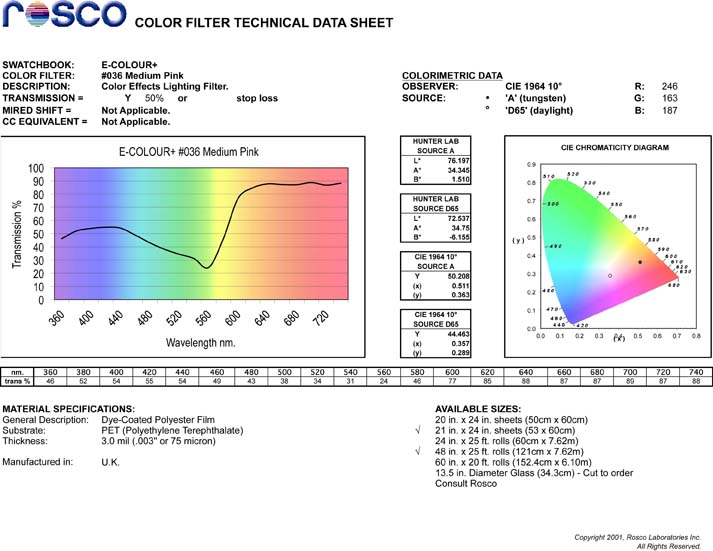
\includegraphics[width=\linewidth]{media/E036_Spec.jpg}
    \caption{Specification Sheet for Filter 'E036'}
\end{figure}

We utilize a web scraping script to pull the spec sheets of all 494 filters from the MyColor tool and approximate the spectral response functions from the chart. 
We compute a transmission function estimate from the attached spec sheet for each filter, and save the transmittance at each discrete wavelength $\lambda$ within $\omega$ denoted as $\omega_d = \{400,401,...750\}$

\begin{figure}[H]
    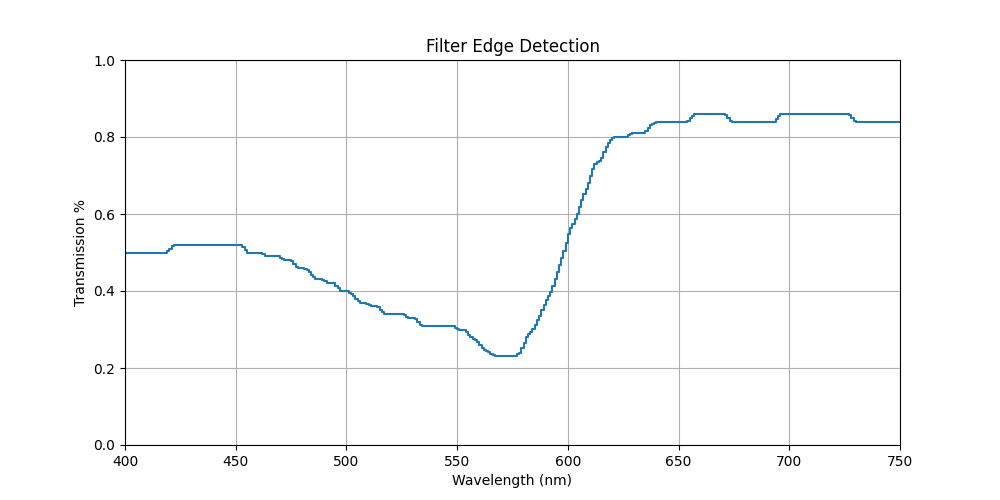
\includegraphics[width=\linewidth]{media/E036.png}
    \caption{Spectral transmission function for $\lambda \in \omega_d$ for MyColor tool filter 'E306'}
\end{figure}

We utilize a similar approach for our simulated camera, acquired from Arducam \cite{arducam_ov9281}. 
The various specification sheets generally provide full cover over $\omega_d$. 

\begin{figure}[H]
    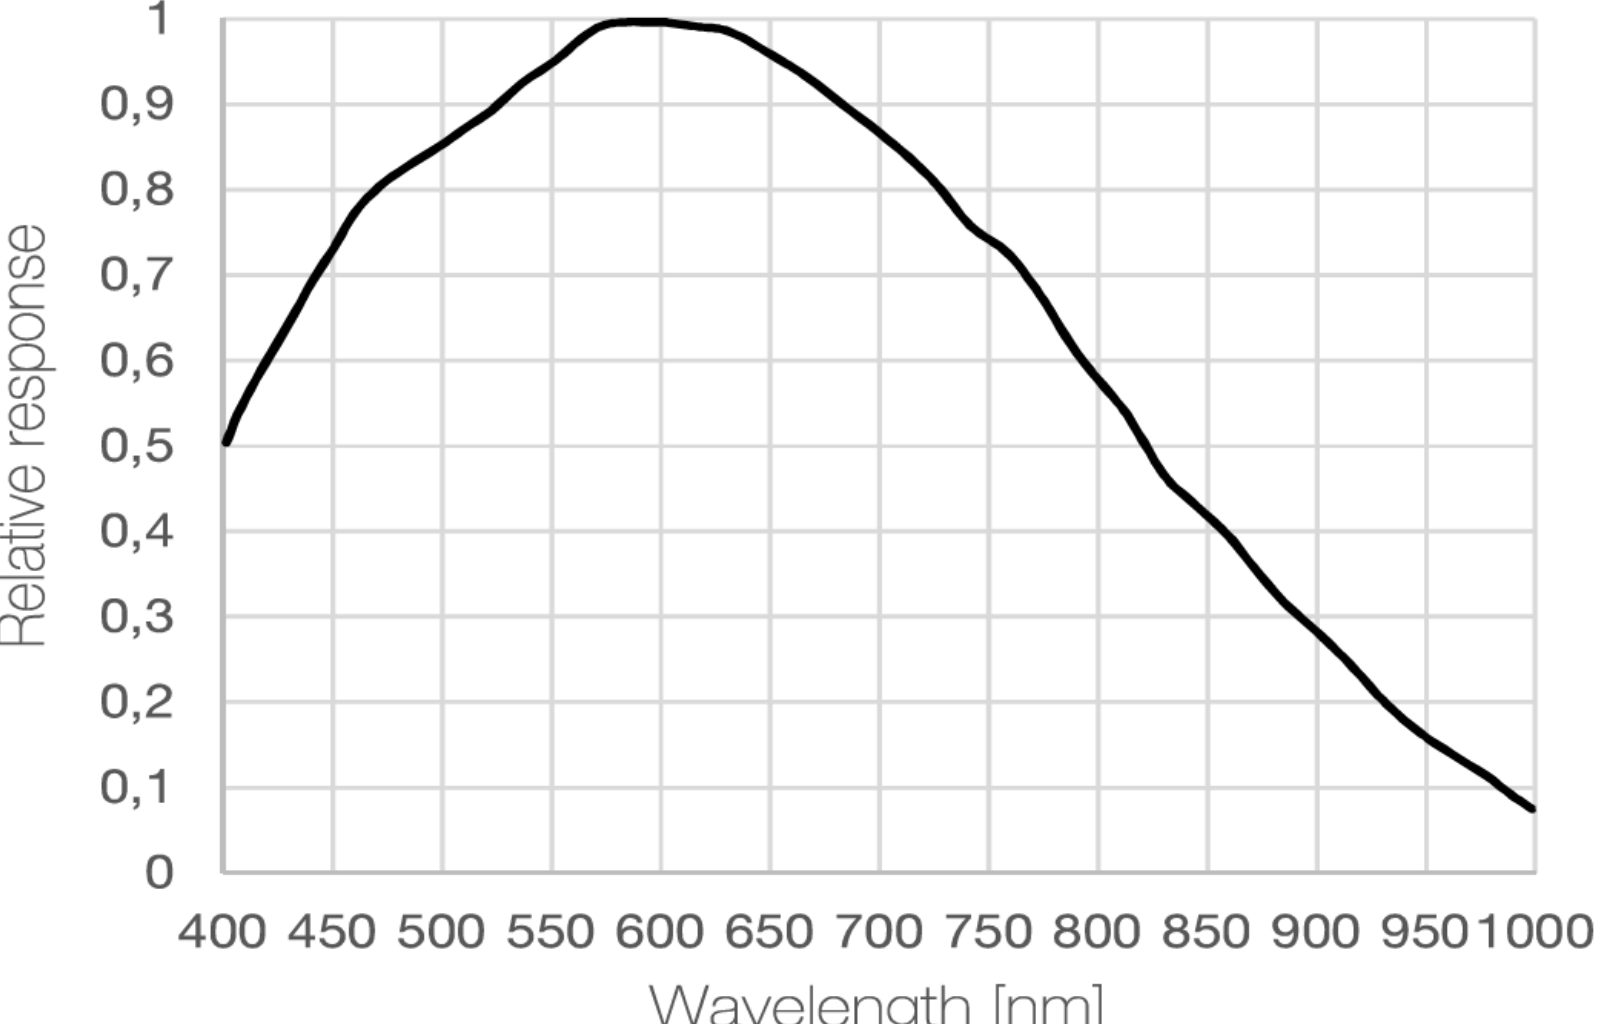
\includegraphics[width=\linewidth]{media/RaspberryPi_trans.png}
    \caption{Monochrome camera transmission function for $\lambda \in [400,1000]$}
\end{figure}

The simulated set of 494 filters from the MyColor tool cover a large space, useful for finding a best-case-scenario when nearly unconstrained by transmission function. 
In reality, we have a set of 119 filters to choose from, which will be sufficient for practical results.
We use a dark room, Lilliput lamp \cite{UtopiaCamLiliput}, and a spectrophotometer to measure the transmission functions of our set of filters. 

\begin{figure}[H]
    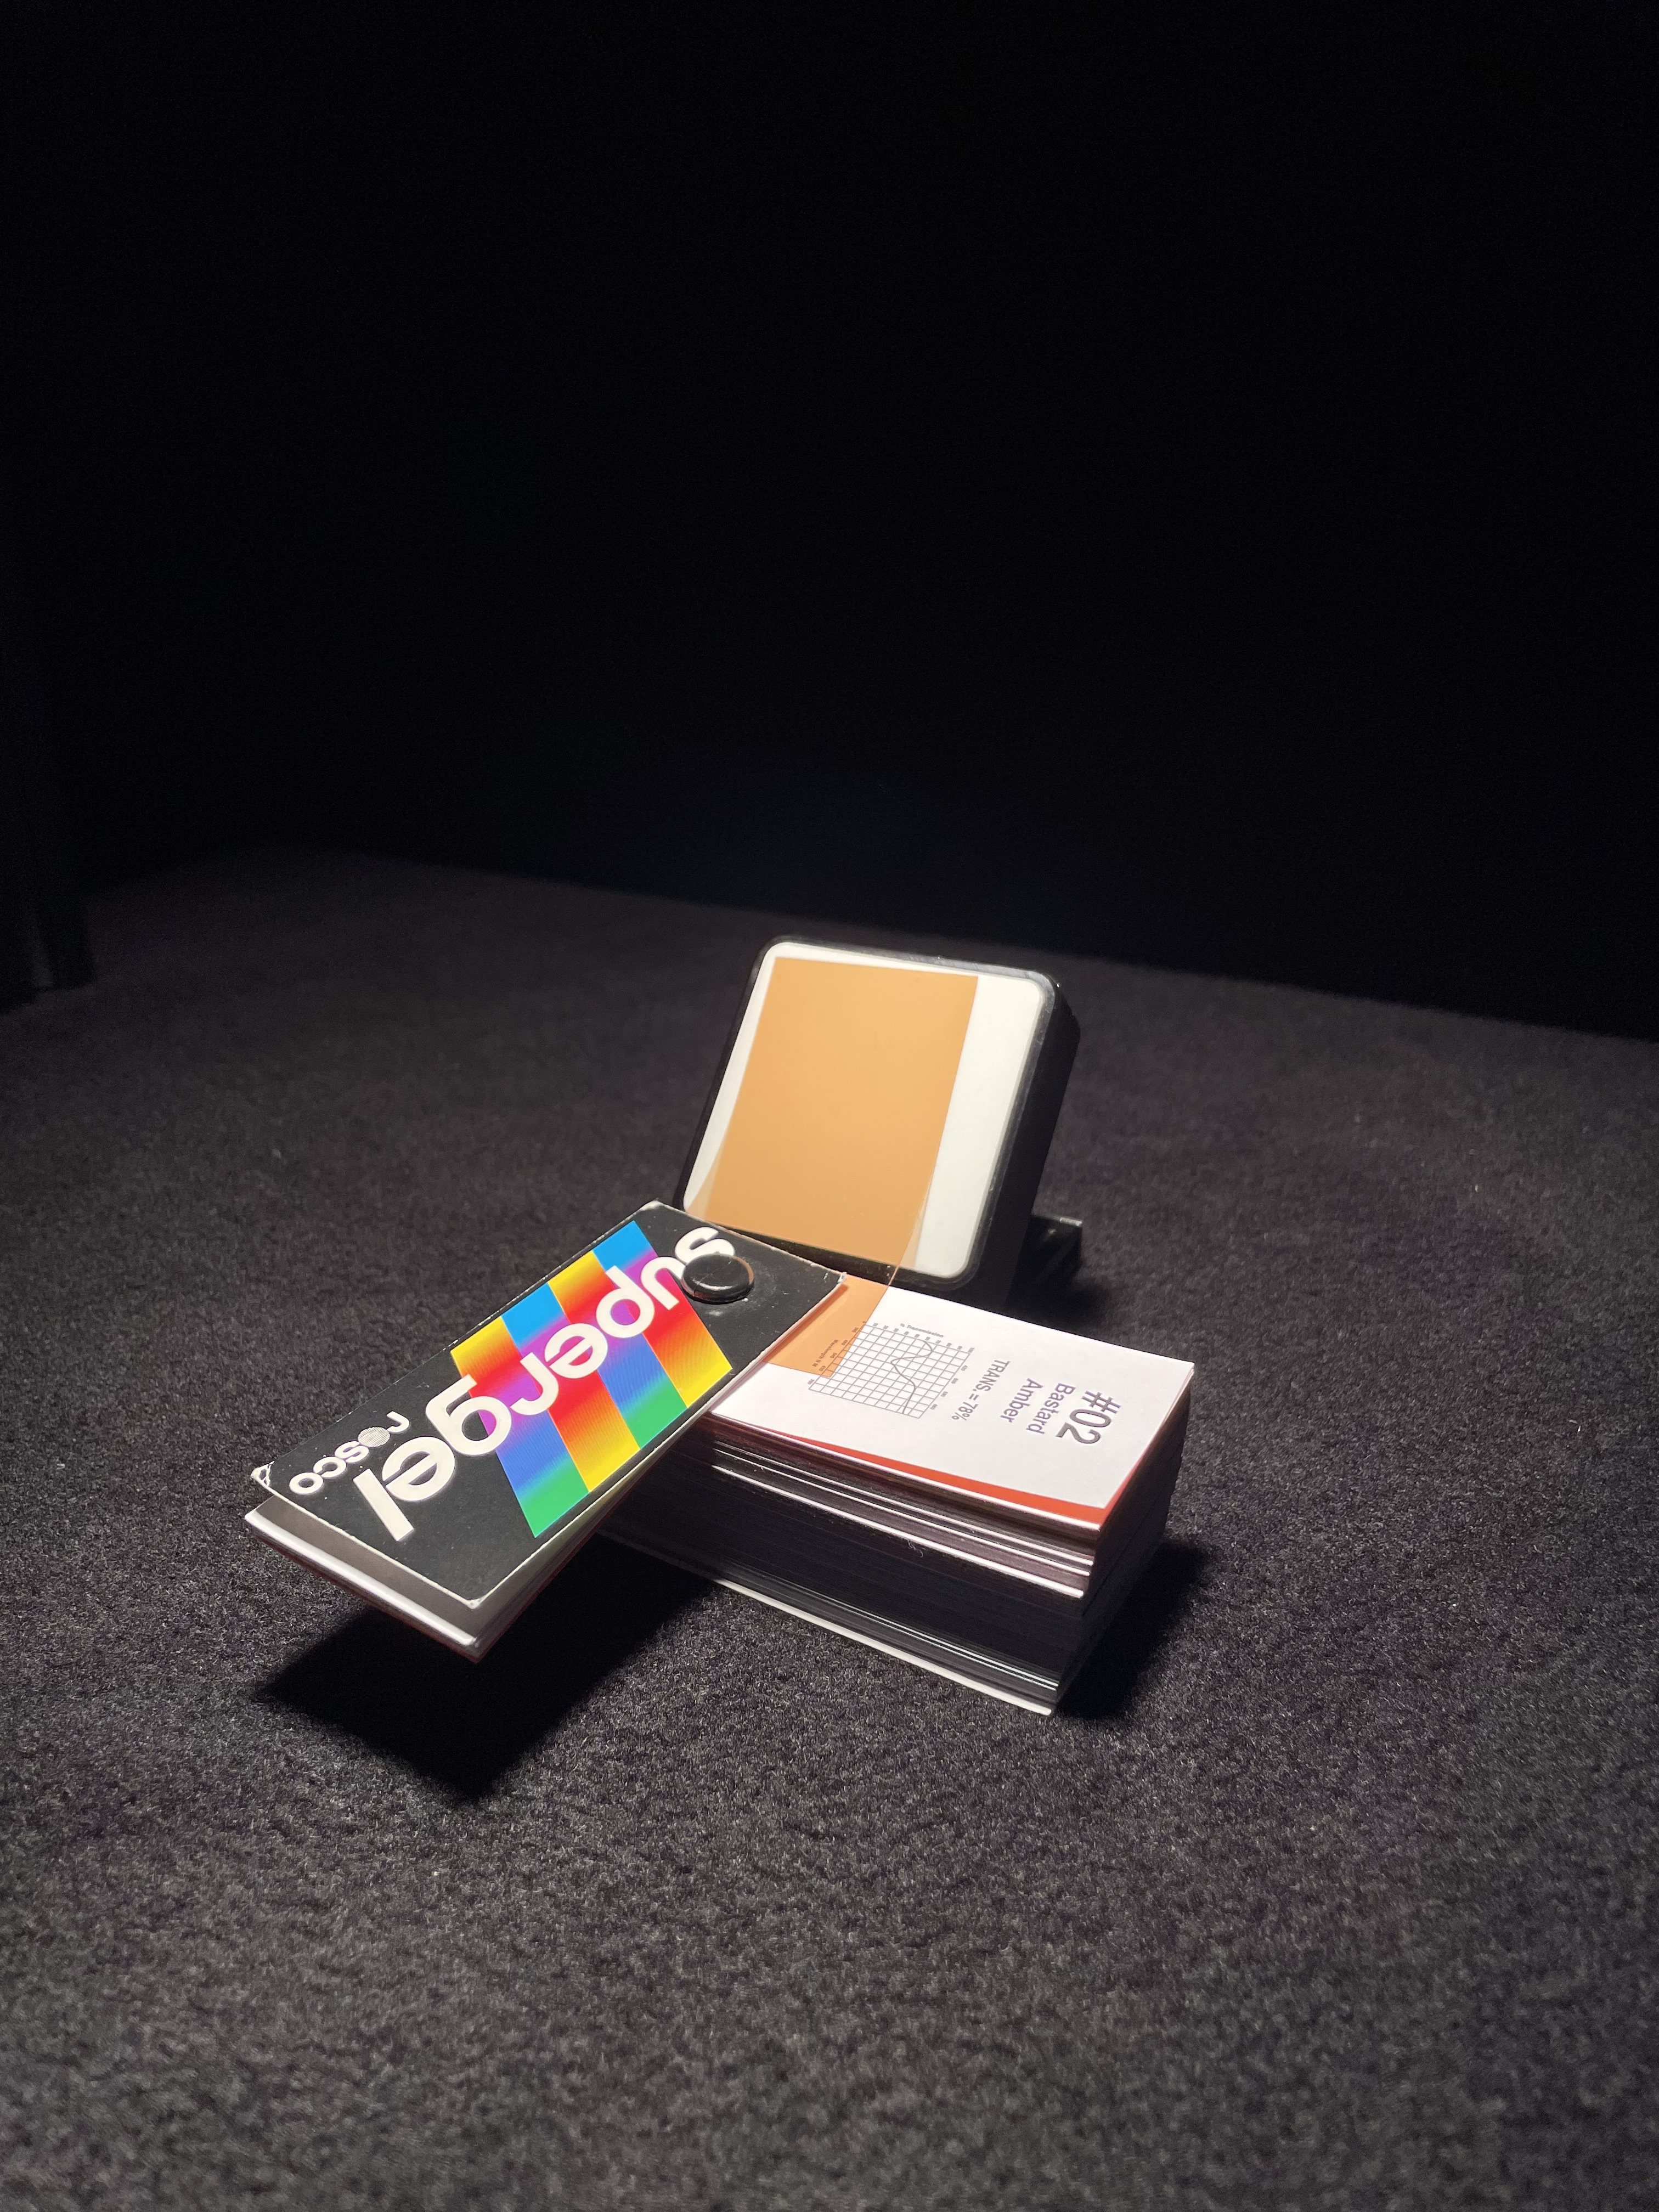
\includegraphics[width=\linewidth]{media/Gels.jpeg}
    \caption{Set of 119 Supergel Filters with \#02 on stage}
\end{figure}

We set up a stage consisting of an overhead illuminant, a reflective surface placed at a 45º angle, and a spectrophotometer pointed at the stage. 
The stage is placed at a 45º angle to the lamp above, with the spectrophotometer aimed at a flush angle to the stage.
The spectrophotometer takes a luminance reading at each wavelength from 350-1000, as well as a measurement of $x$ and $y$, from which the XYZ color coordinates may be derived. 
For this case, we are interested in calculating the transmission function of each filter, so we care about the luminance reading, but further applications of the spectrophotometer, specifically the $x$ and $y$ reading will be discussed below. 

\begin{figure}[H]
    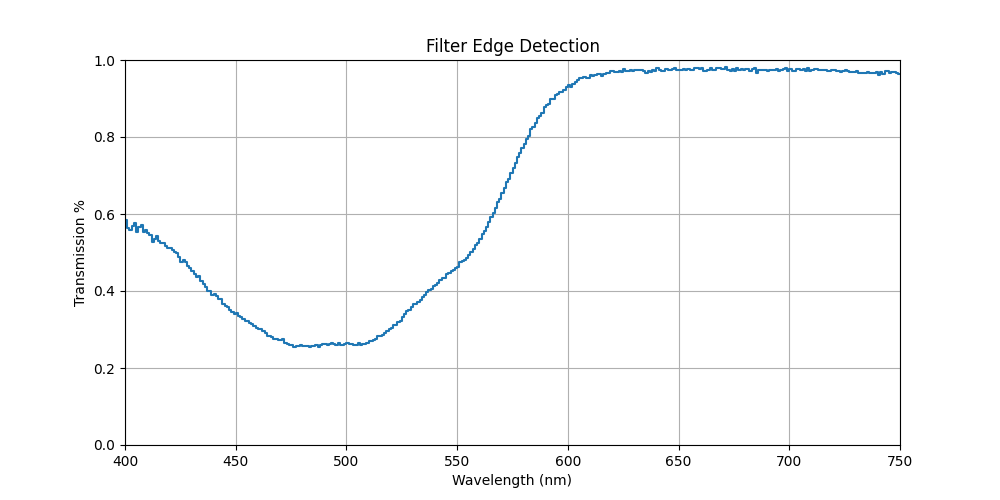
\includegraphics[width=\linewidth]{media/304.png}
    \caption{Measurement of Supergel filter \#304 for $\lambda \in \omega_d$}
\end{figure}

Brightness in the room was controlled by covering the walls with black felt and ensuring that the computer monitor was pointed away from the stage. 
The spectrophotometer is equipped with a laser to ensure accuracy in measurement, and each filter was placed flush against the stage for measurement. 

\begin{figure}[H]
    \includegraphics[width=\linewidth]{media/measure2labeled.jpeg}
    \caption{Filter measurement setup with spectrophotometer and Rosco Supergel filters.}
\end{figure}

The stage and illuminant can be seen on the left below, with the control panel and transmission function readout on the right. 
The results of each scan are saved into a $.mat$ file at 1 nanometer increments, along with a few calibration runs with no filter present.

\begin{figure}[H]
    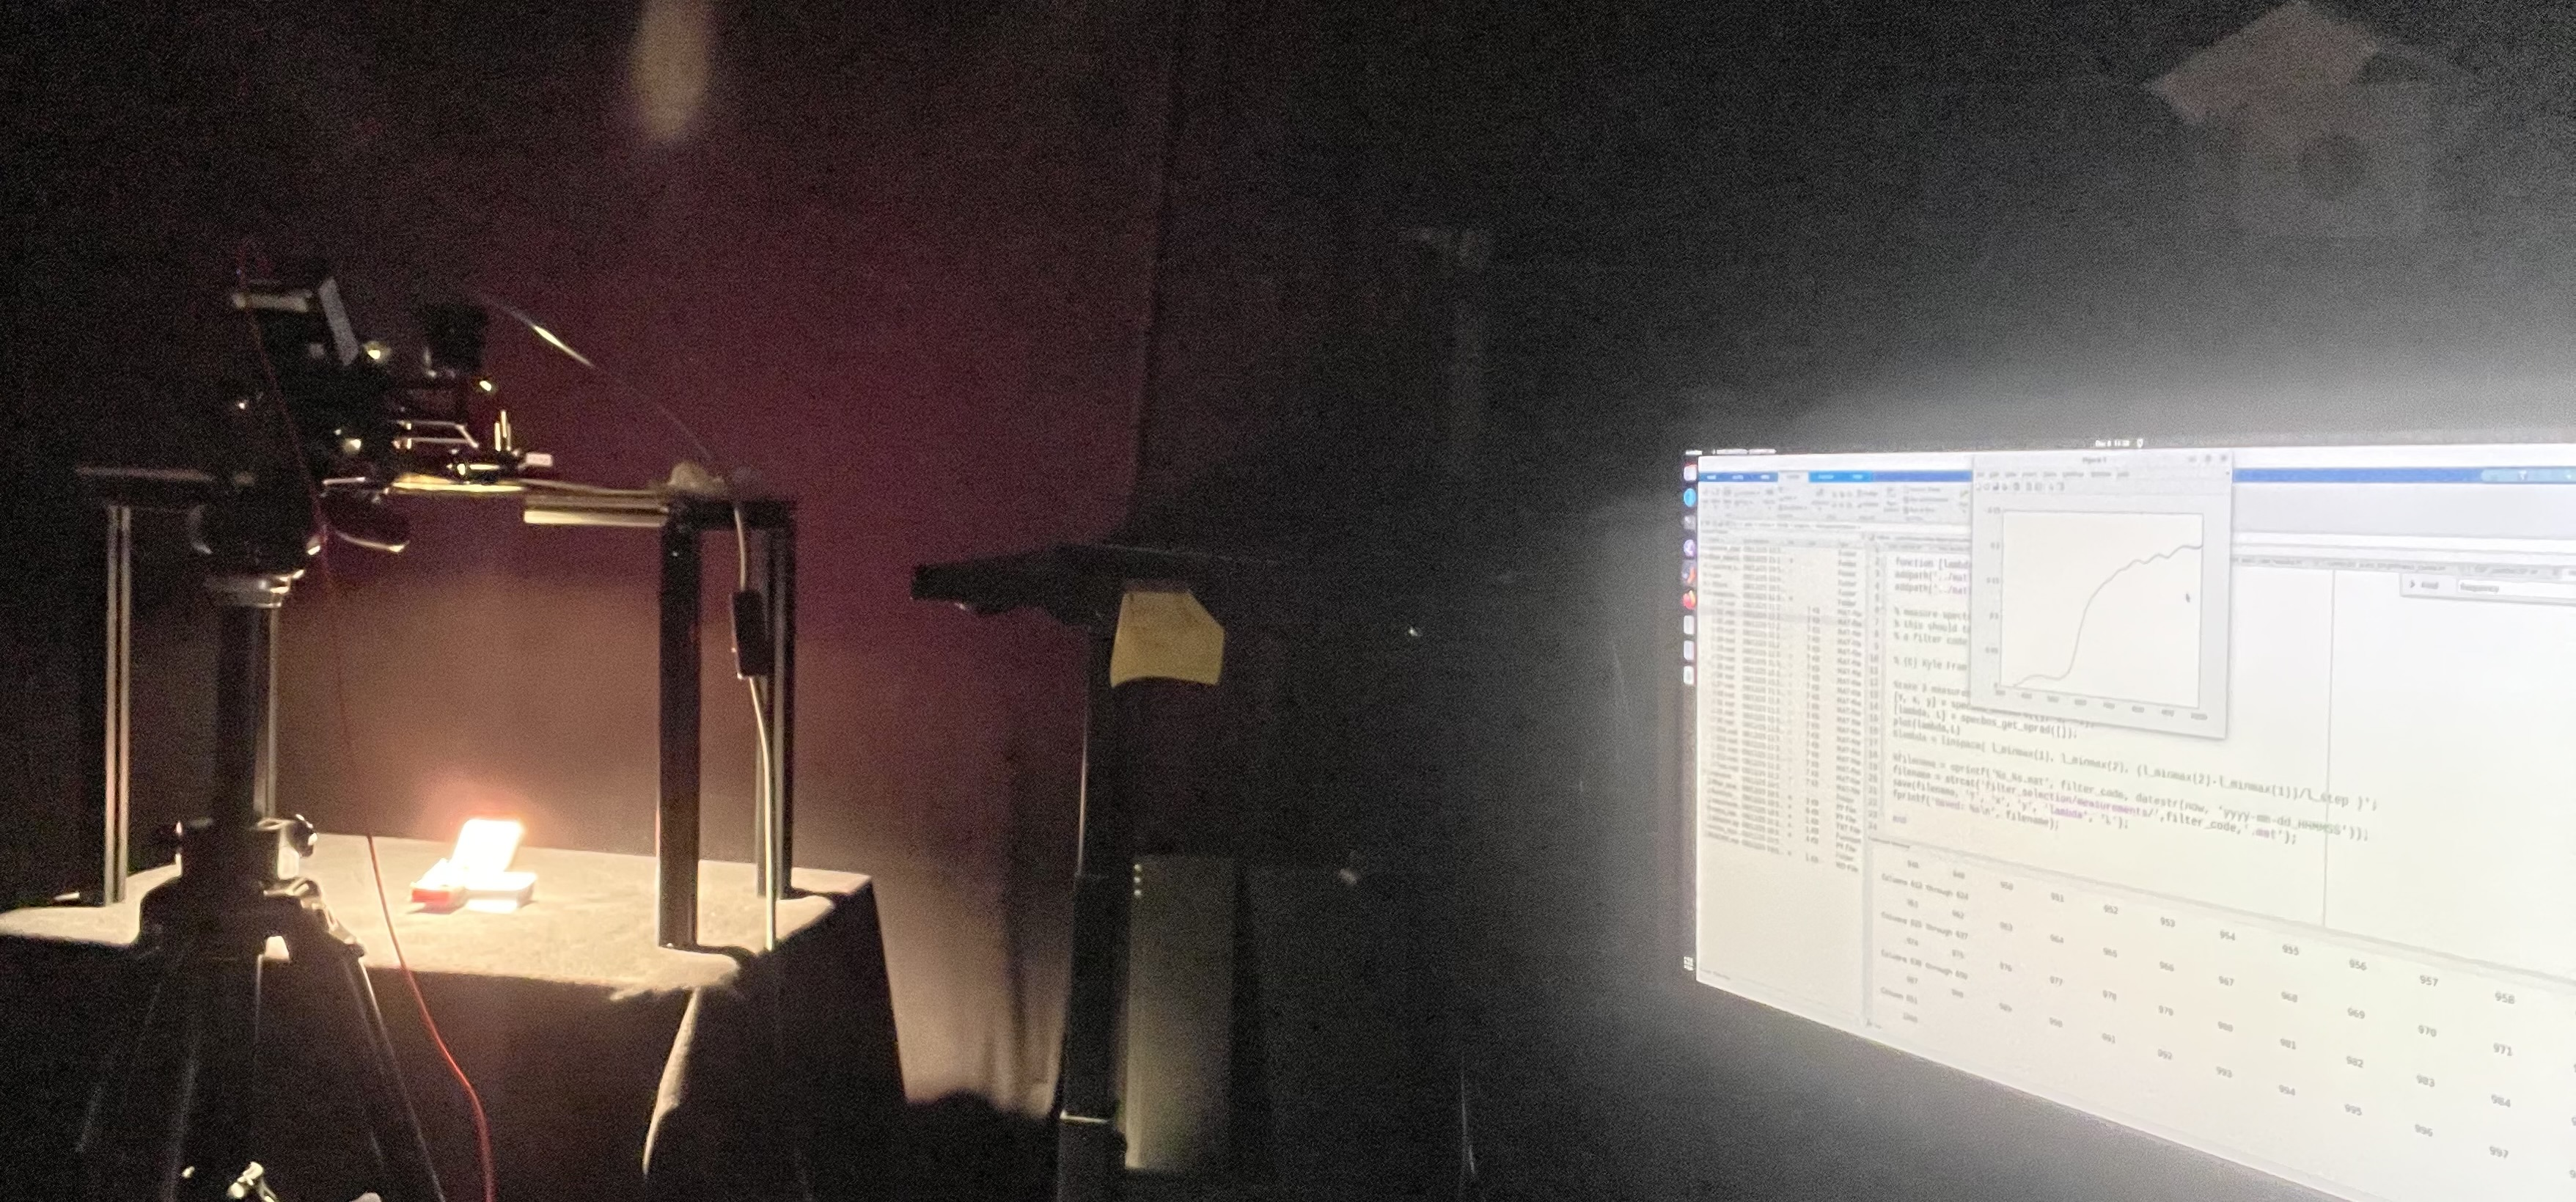
\includegraphics[width=\linewidth]{media/Measure3.jpeg}
    \caption{Computer readout of spectrophotometer measurement in dark room}
\end{figure}

For our target functions, we utilize the UCL Color \& Vision Research Laboratory repository of cone and rod sensitivity functions \cite{CVRL}, including CIE XYZ 1931 and CIE 2006 LMS functions (transformed to XYZ for consistency).

We also benchmark our performance by computing $\Delta E_{2000}$ using the RGB coordinates of the Macbeth ColorChecker as per Pascale \cite{Pascale2006RGBCO}. 
For a demonstration of color reconstruction across scenes, we utilize the CAVE dataset from Yasuma et al. \cite{yasuma2010generalized}

\begin{figure}[H]
    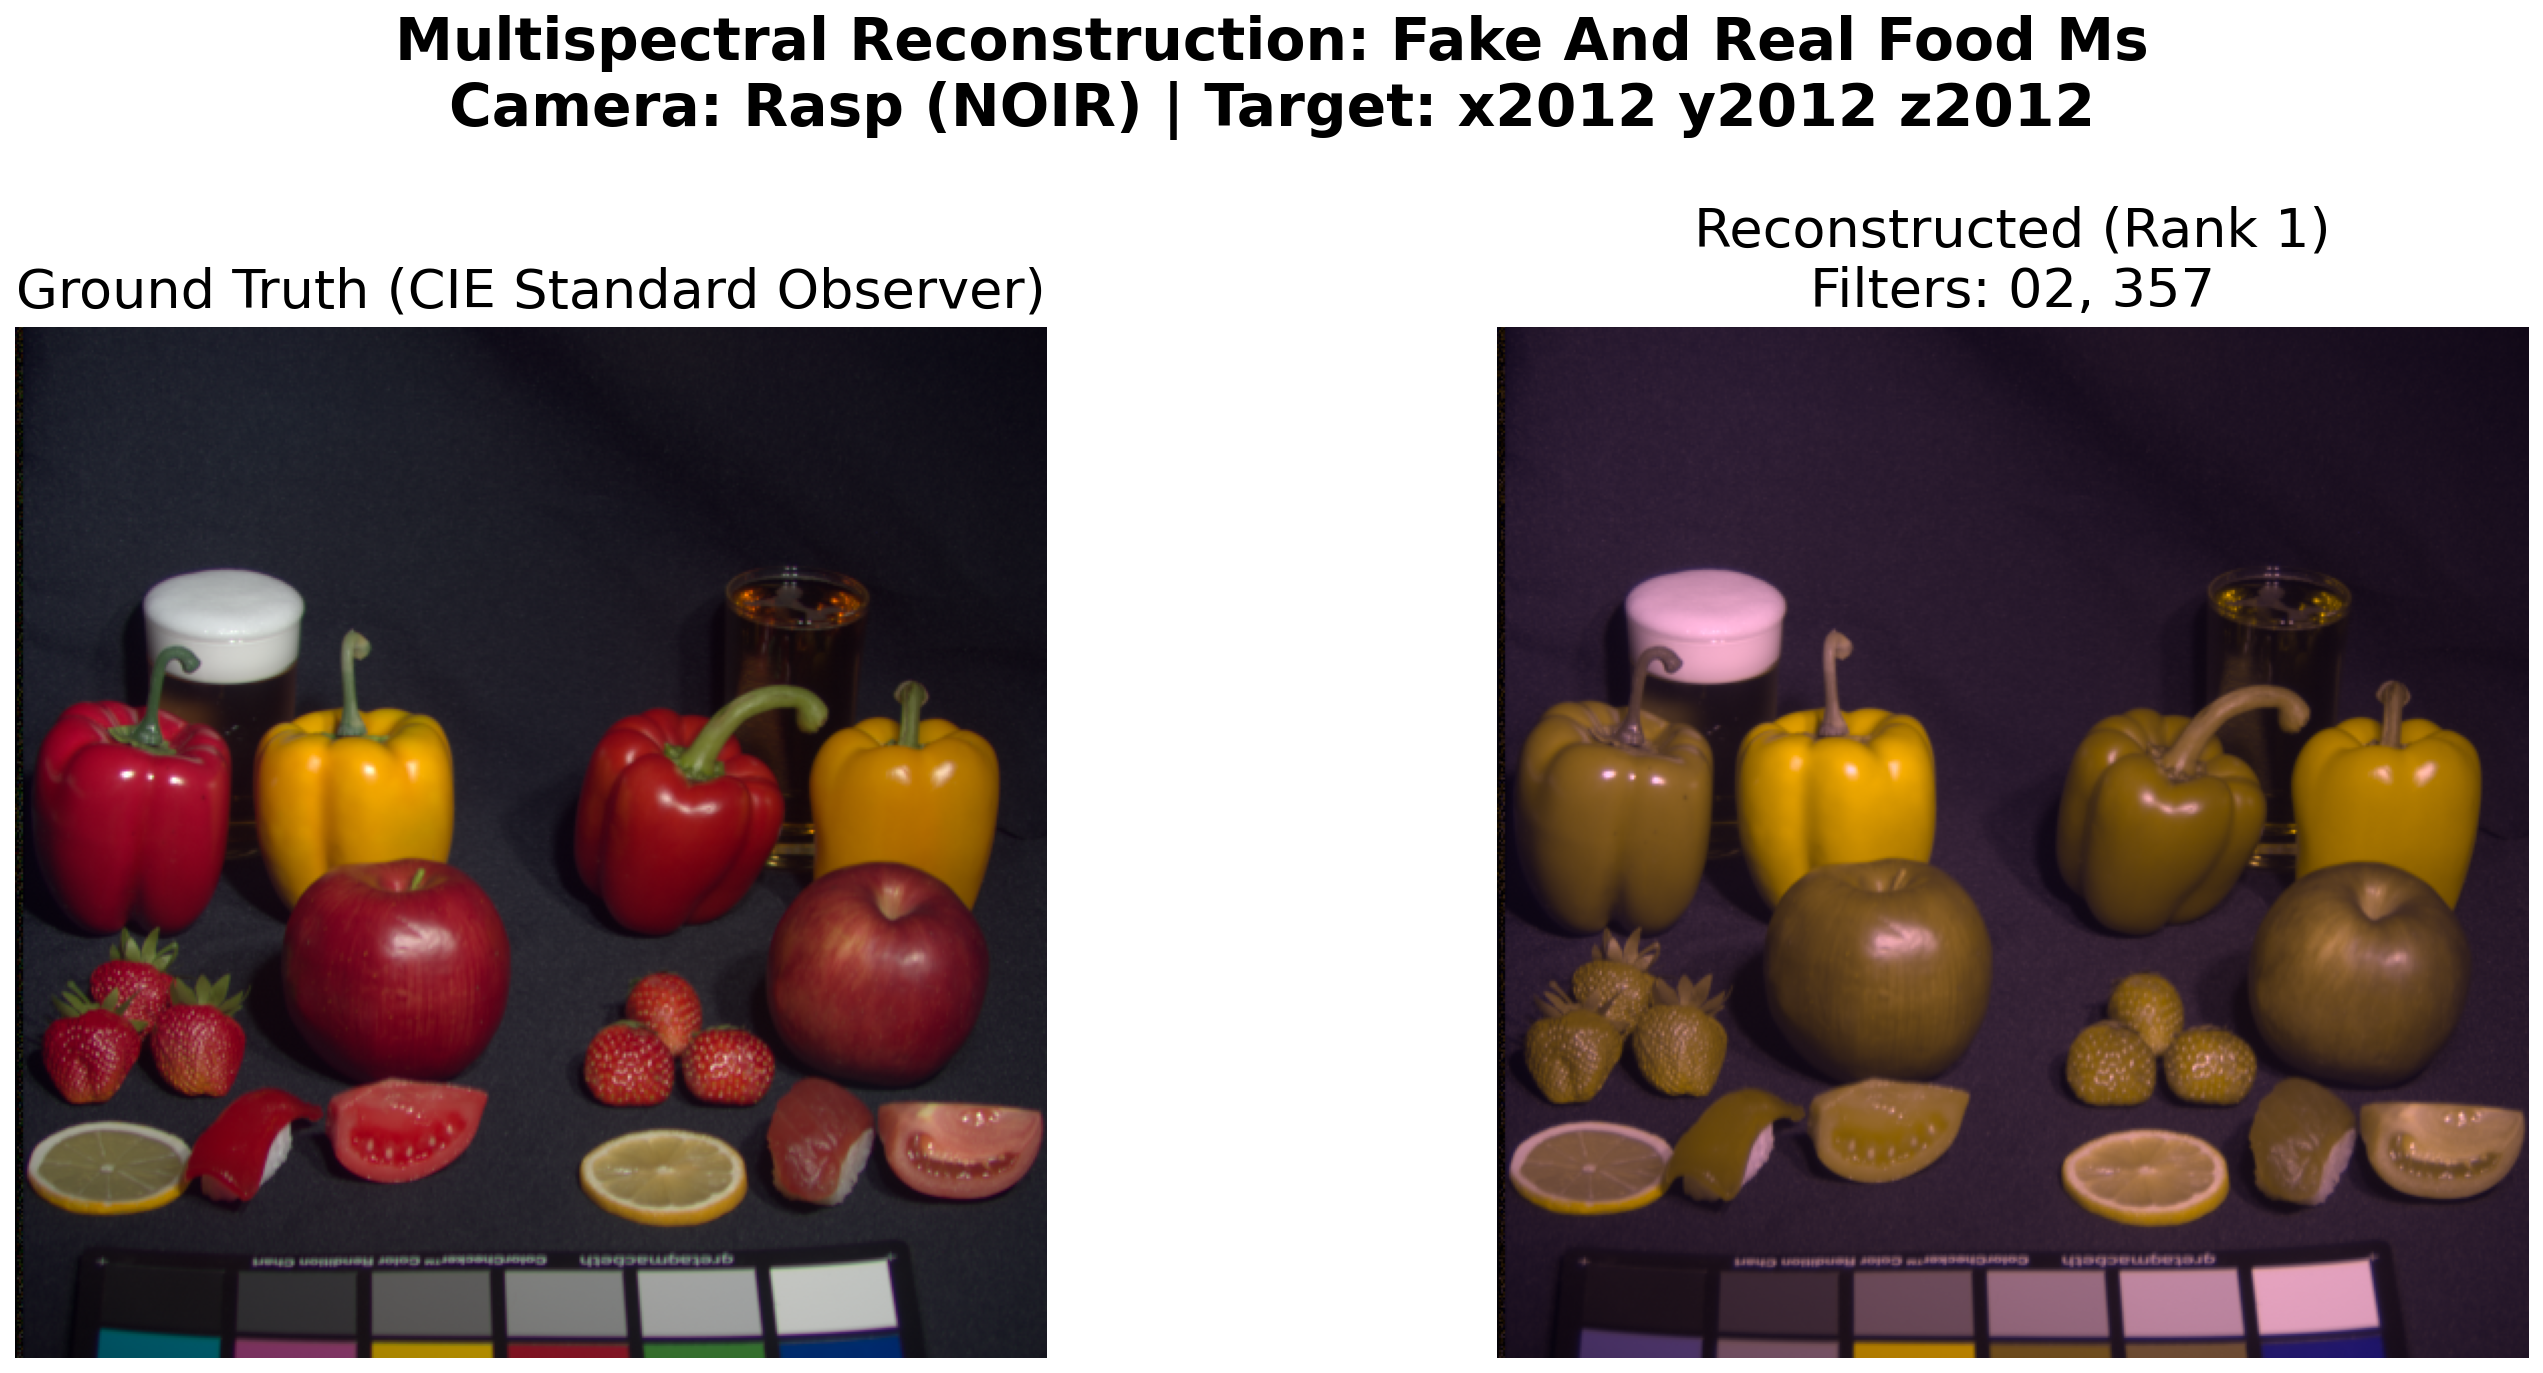
\includegraphics[width=\linewidth]{media/Cave_DataCollection.png}
    \caption{Example of a simulated reconstruction from the CAVE dataset for $k=2$ filters}
\end{figure}

Next, we replicate the above simulated spectral reconstruction in the lab, capturing a scene including one Preferred Memory Color Chart \cite{ThouslitePMCC} under the same Lilliput illuminant \cite{UtopiaCamLiliput}.


\begin{figure}[H]
    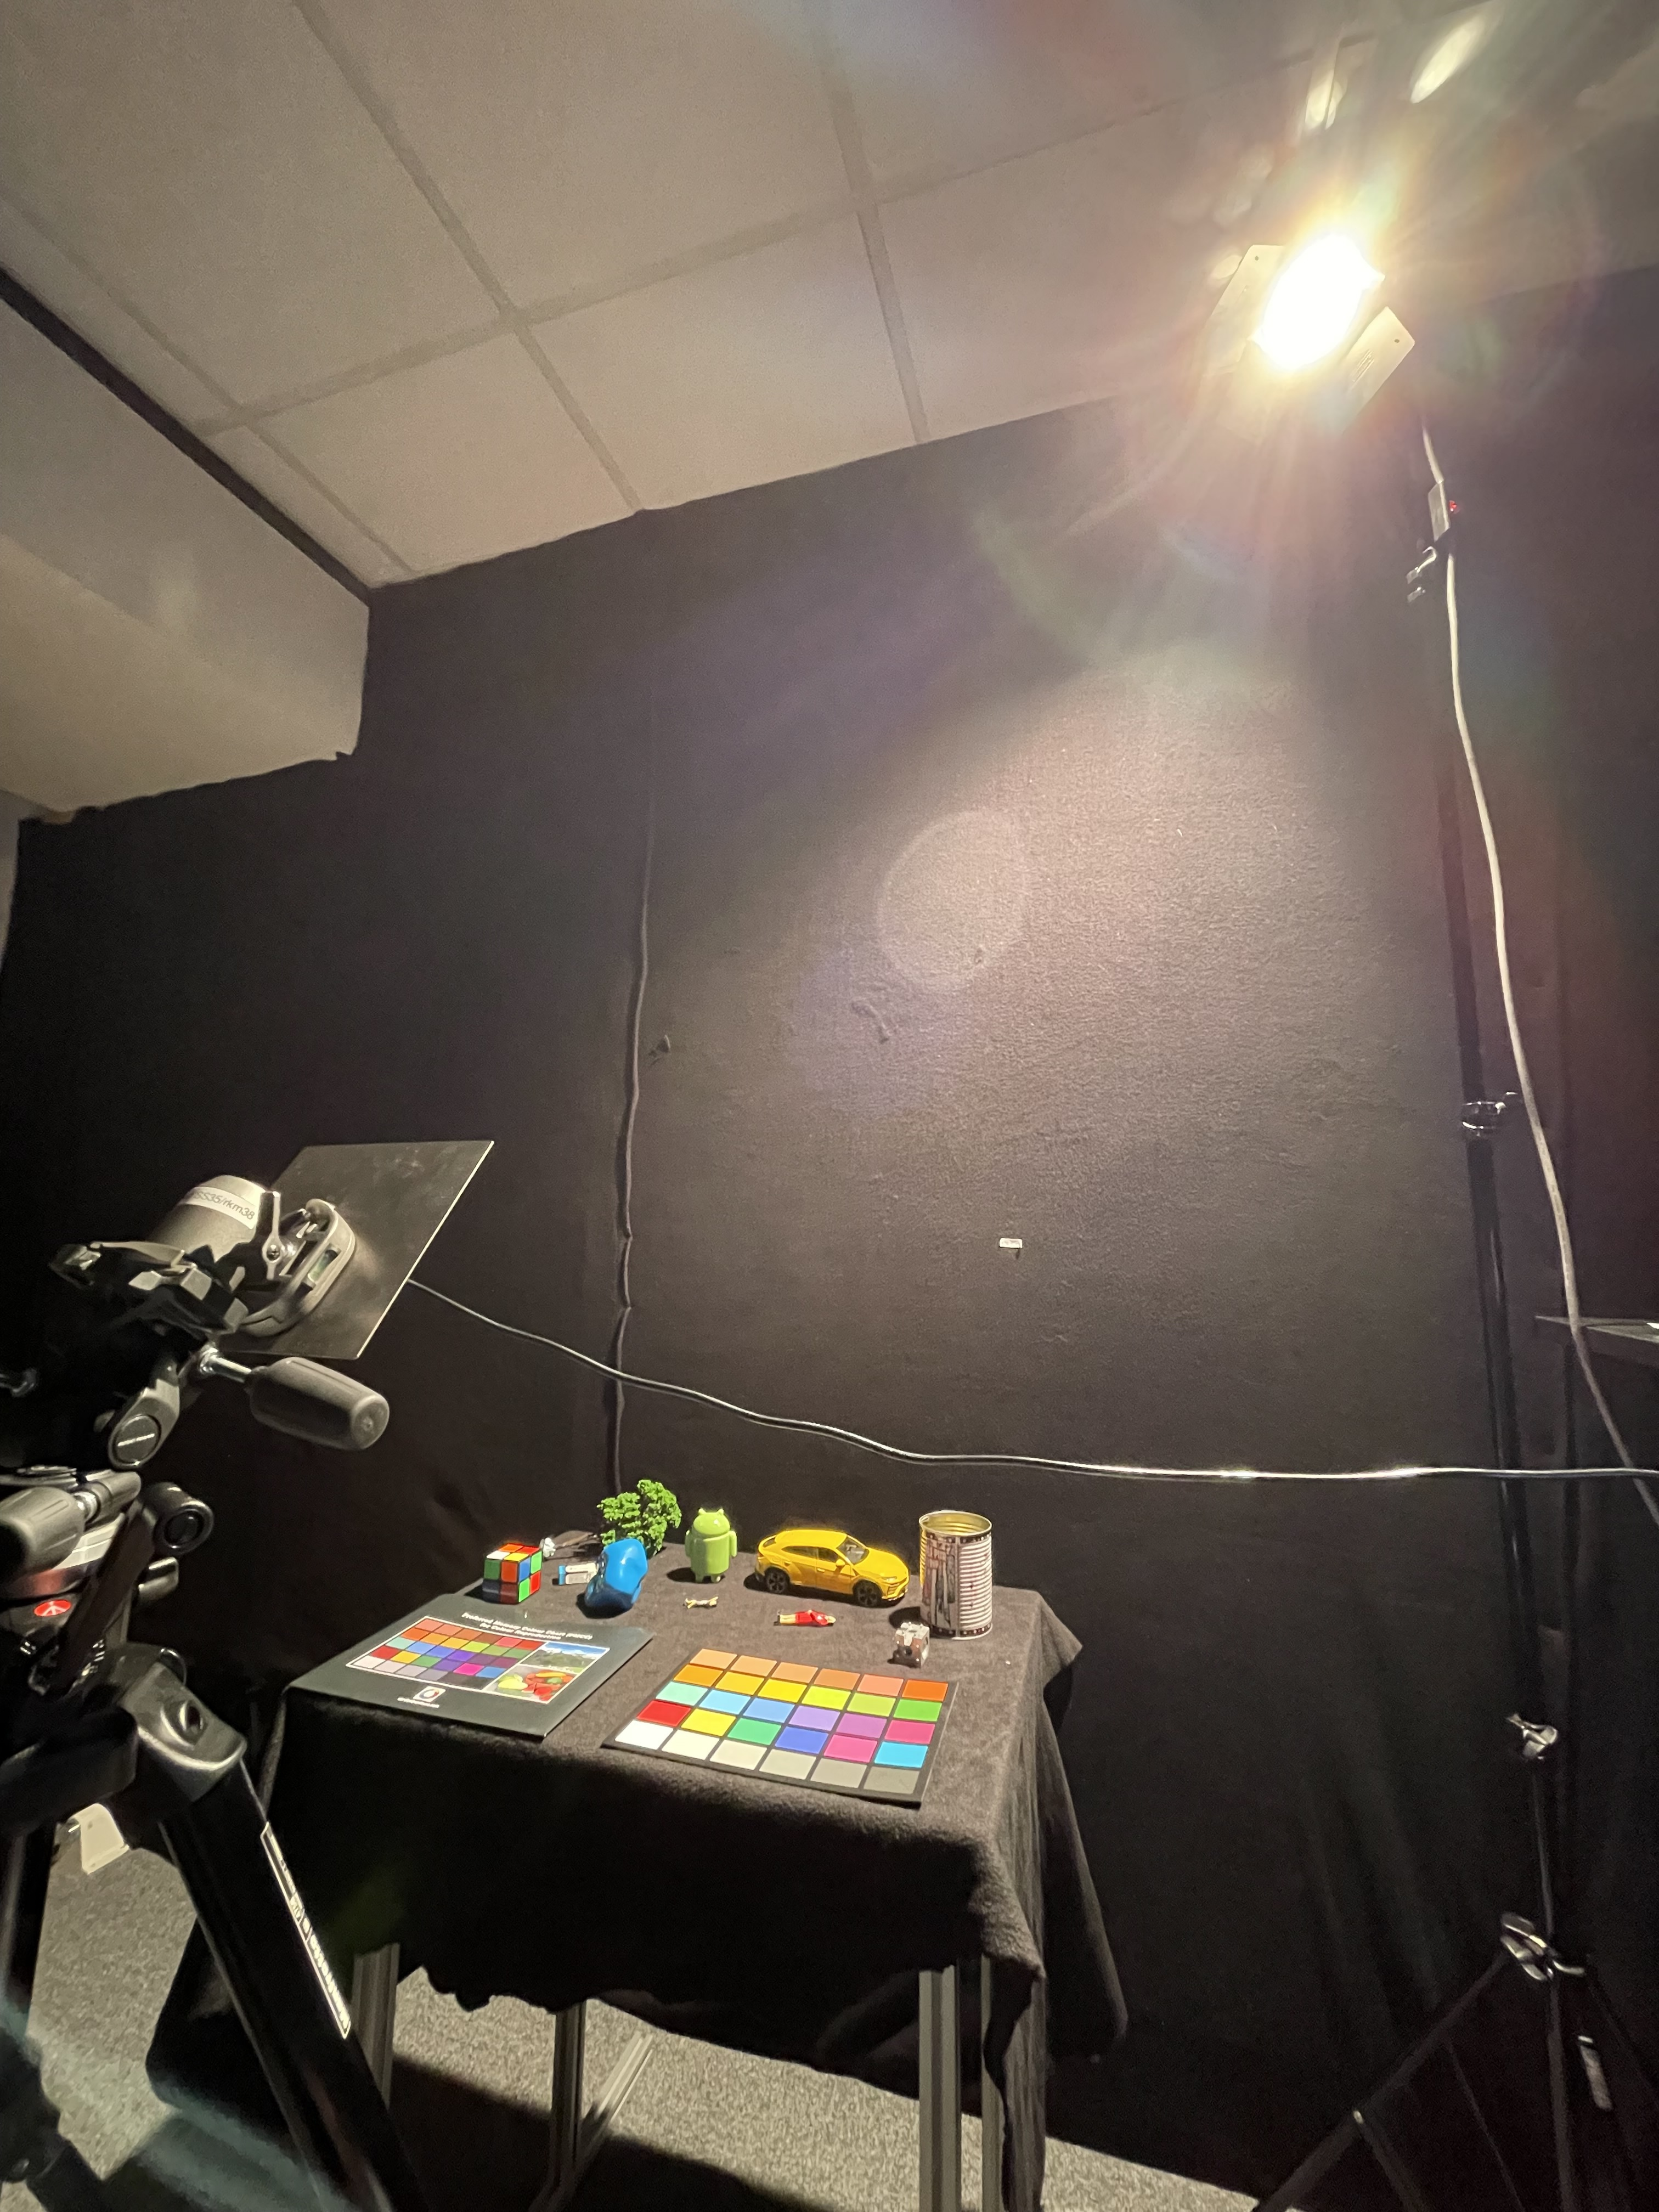
\includegraphics[width=\linewidth]{media/spectralLab.jpeg}
    \caption{Lab setup for multispectral imaging with illuminant}
\end{figure}

To this end, each filter was placed in front of the camera, mounted onto a tripod and aimed at a scene including objects of different reflectances and colors. 
Additionally, the PMCC was placed at the front of the scene for easy quantitative color analysis. 
The camera was kept in place such that we could pick one pixel per capture for which to measure each color patch under each respective filter. 

\begin{figure}[H]
    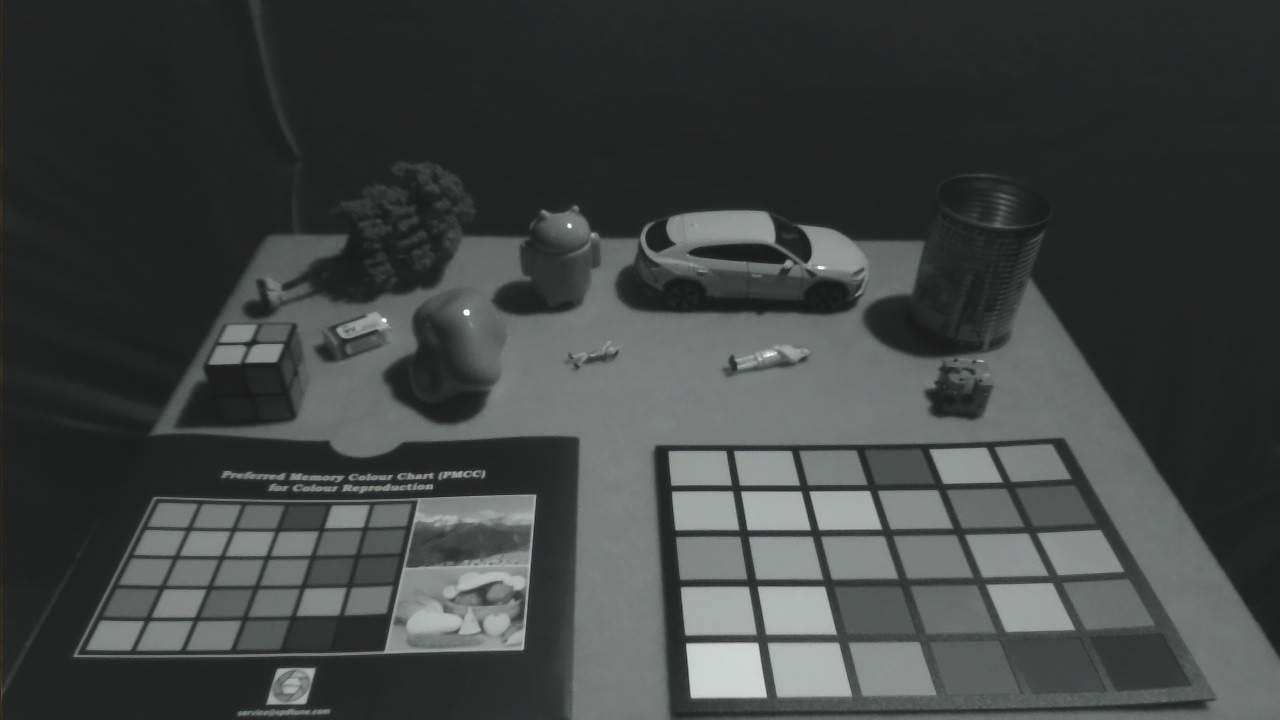
\includegraphics[width=\linewidth]{media/398.jpg}
    \caption{Capture of filter \#398 from monochrome camera, including PMCC in the foreground}
\end{figure}

Other items were placed in frame as well for qualitative reivew, a subset are shown in detail. 

\begin{figure}[H]
    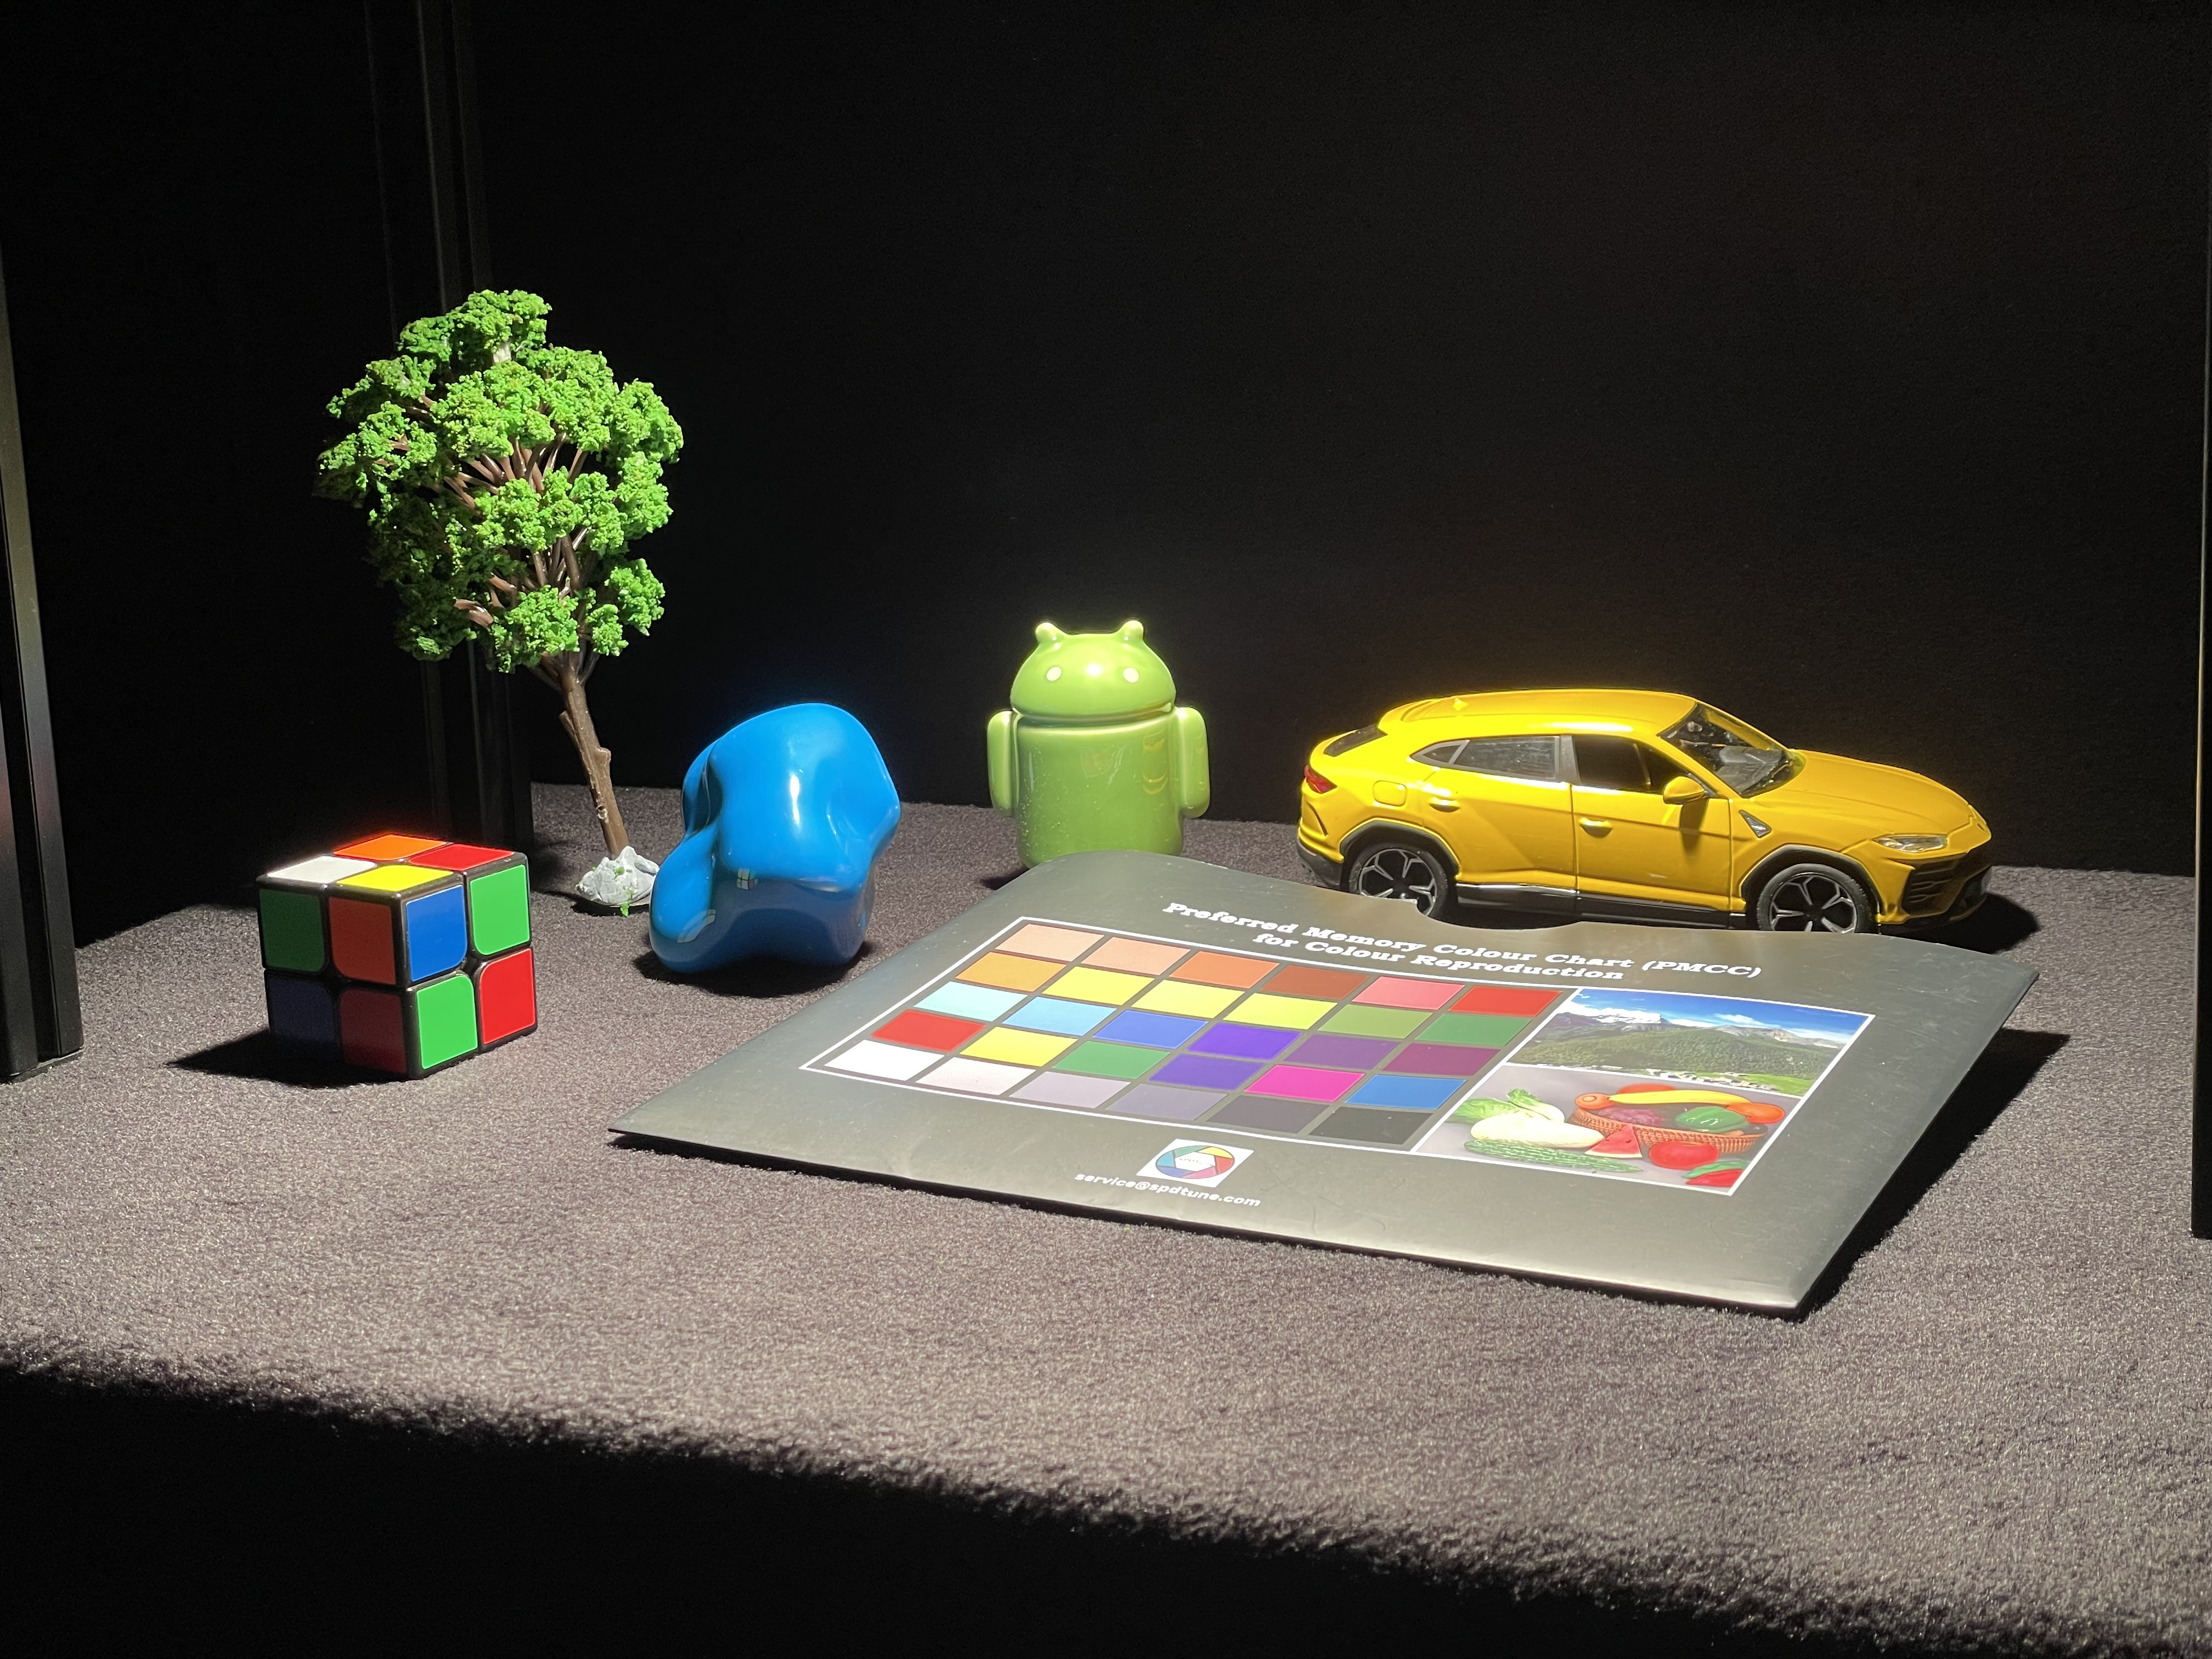
\includegraphics[width=\linewidth]{media/items.jpeg}
    \caption{Subset of items staged for color capture}
\end{figure}

Ground truth measurements were taken with the same spectrophotometer as above, under consistent angular setup and the same lighting. 
Each panel of the SPD was captured in order to compute absolute colorimetric difference between spectral reconstruction and ground truth. 

\begin{figure}[H]
    \includegraphics[width=\linewidth]{media/Spectrophotometer2.jpeg}
    \caption{Items staged for color capture, including a PMC}
\end{figure}

A render of the readings taken with the spectrophotometer is shown, providing a human-eye check that our readings were taken correctly. 
The white patch provided a white point and other patches were rendered after normalizing to this white, taking the illuminant as D65.
\begin{figure}[H]
    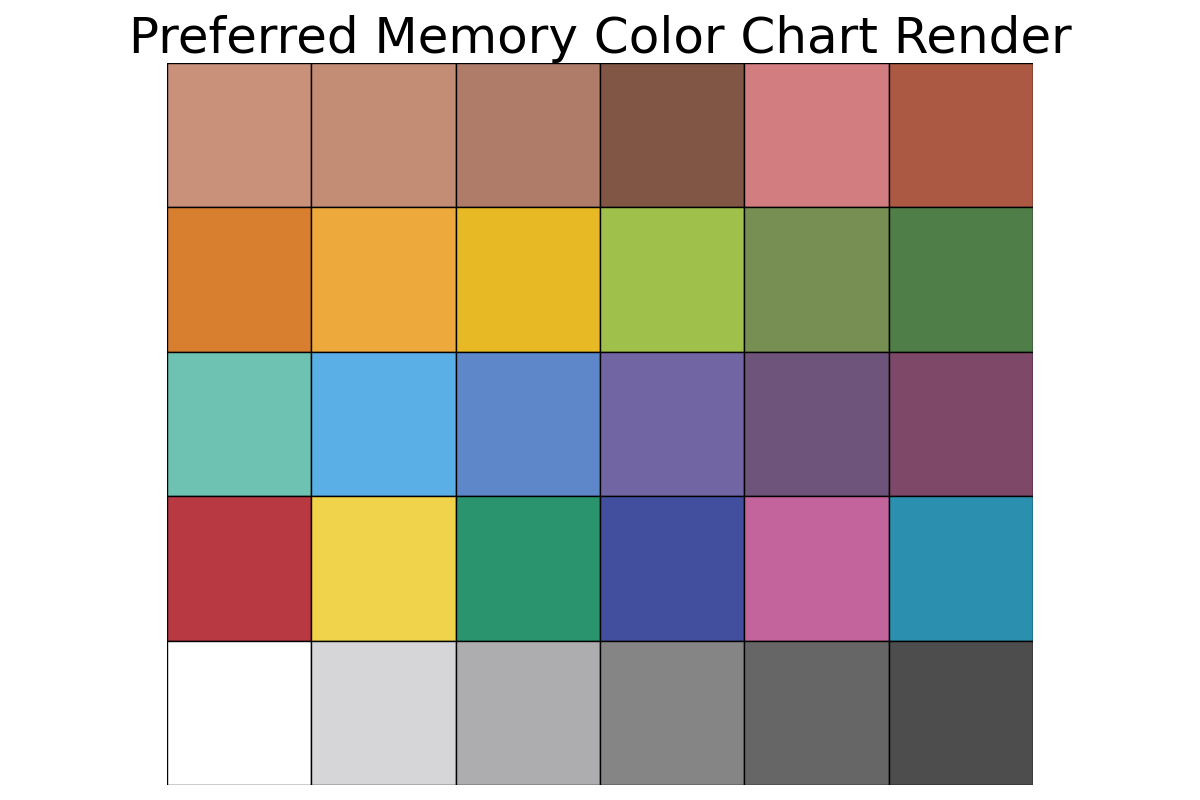
\includegraphics[width=\linewidth]{media/colorcheck_render.png}
    \caption{Render of Spectrophotometer Readings}
\end{figure}

We plot the color patches on the standard XYZ gamut for illustration.

\begin{figure}[H]
    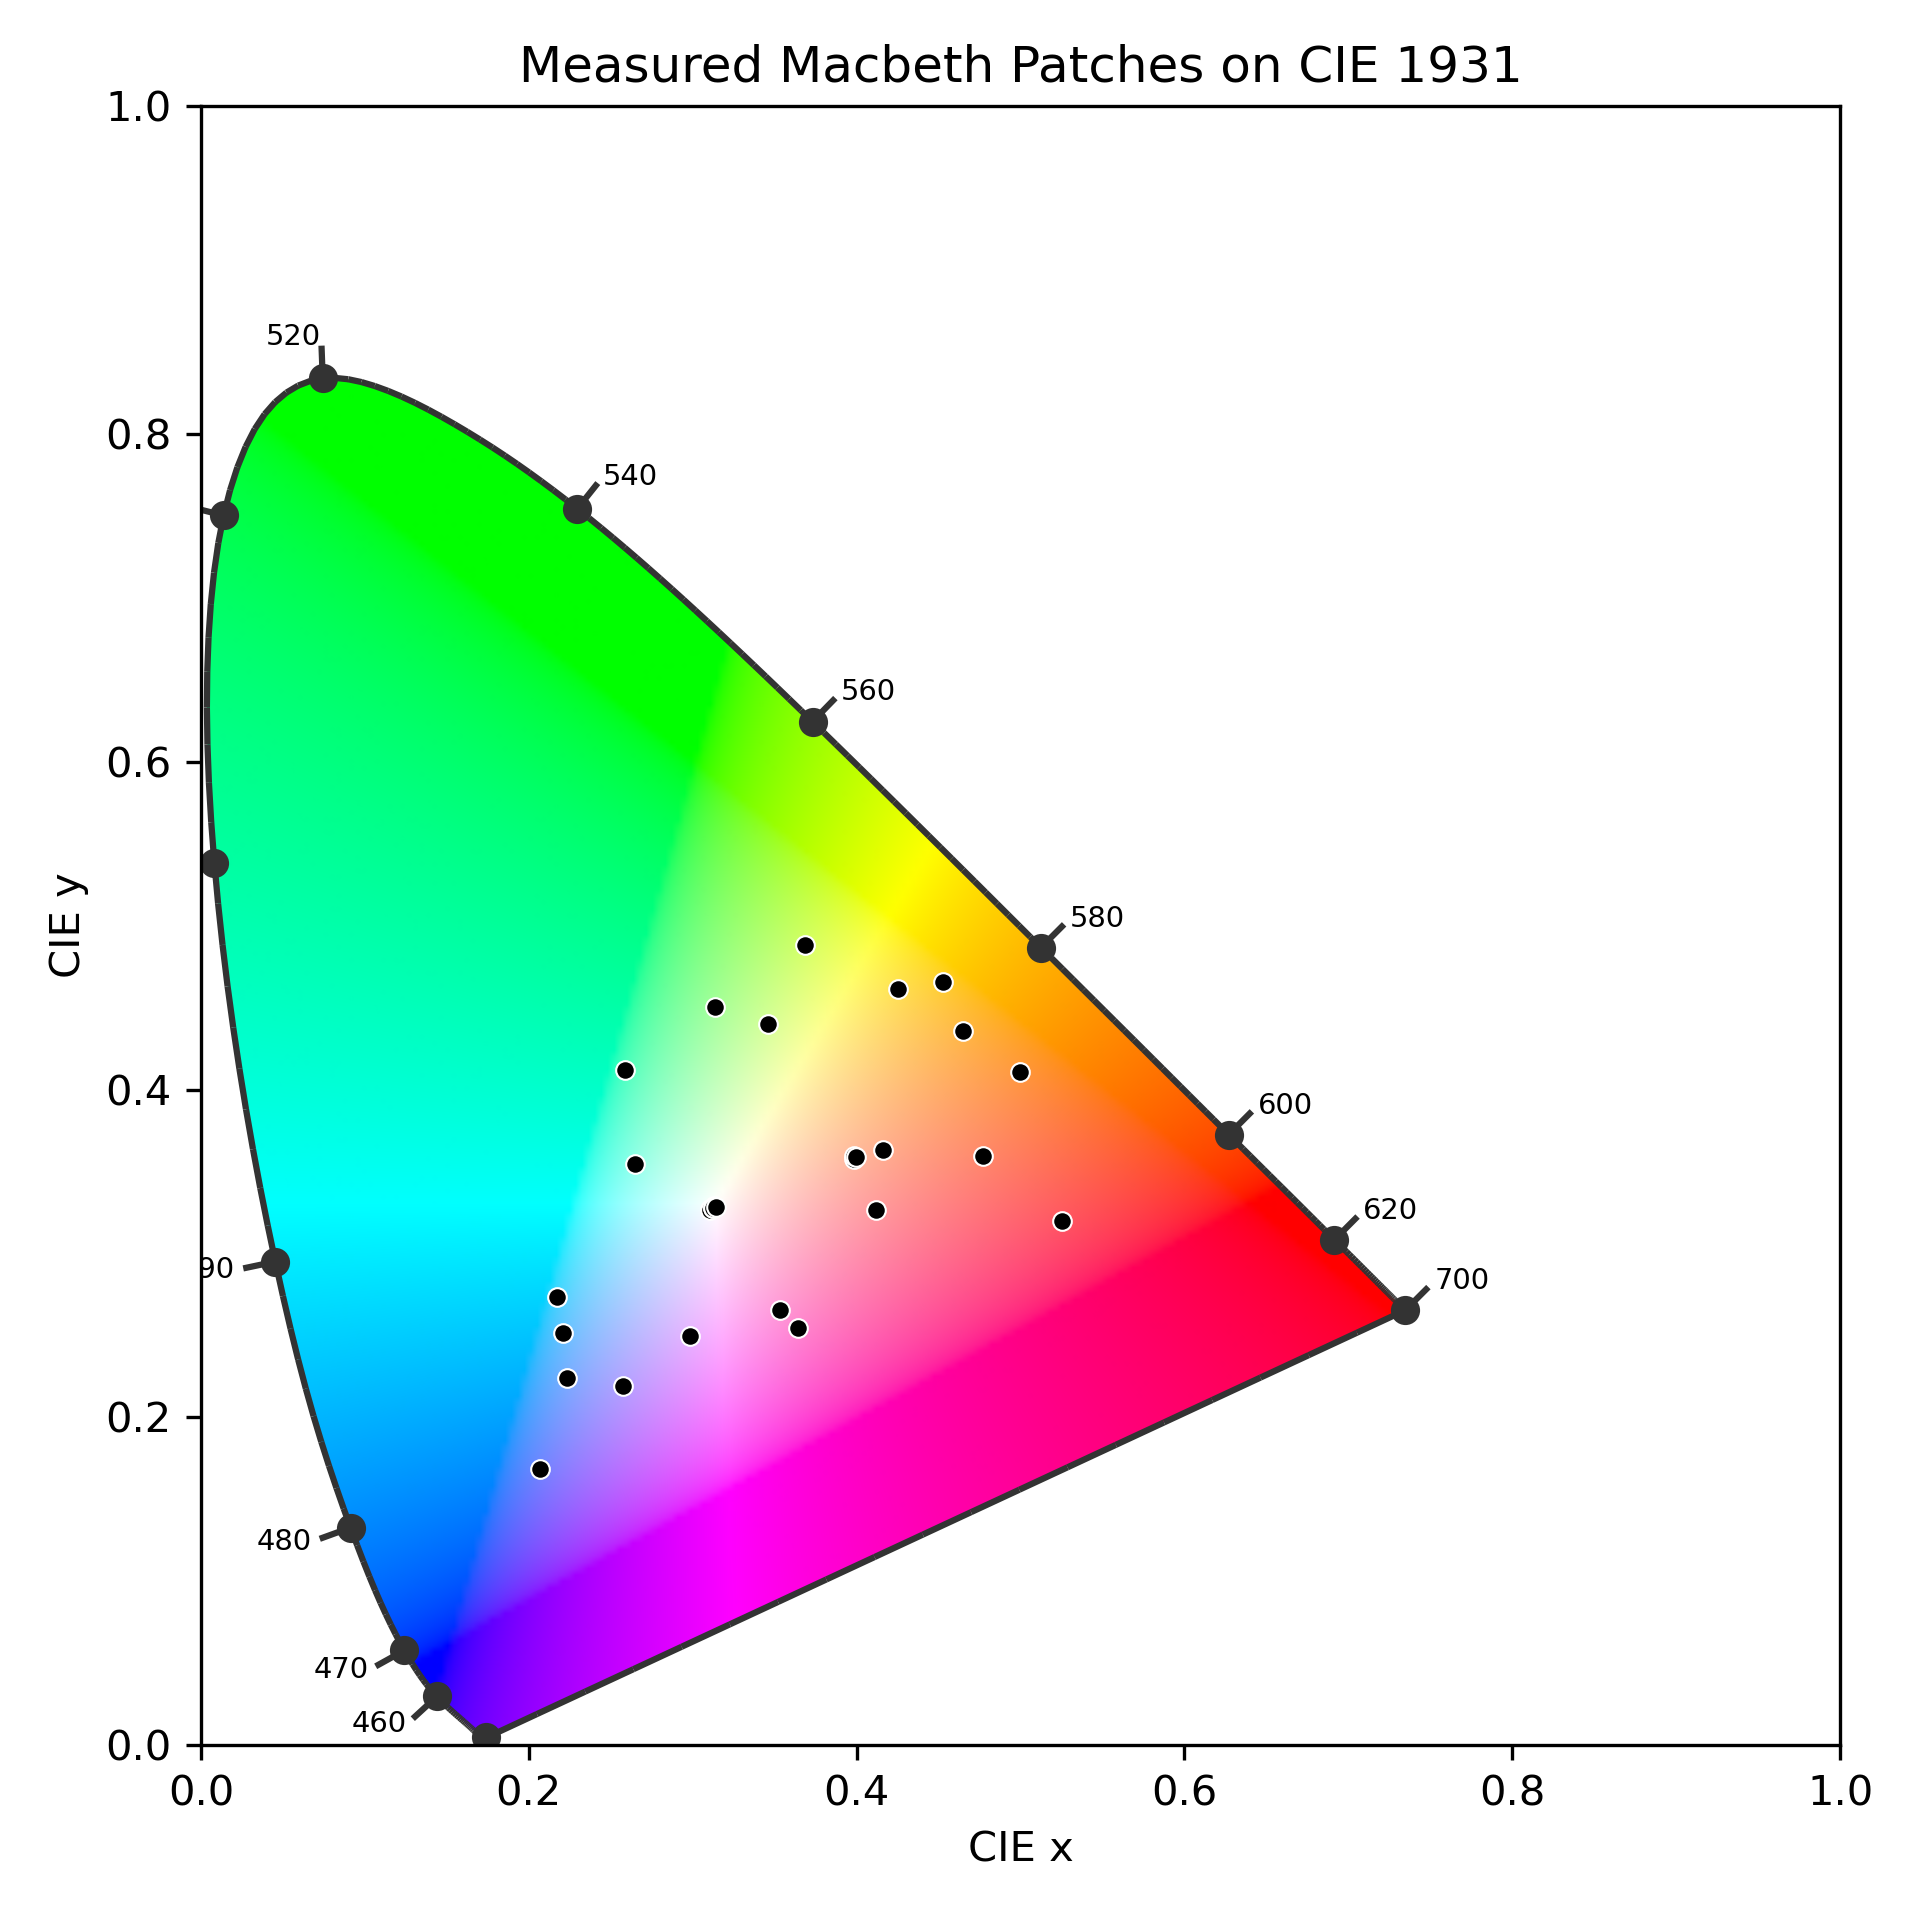
\includegraphics[width=\linewidth]{media/colorcheck_chromacity.png}
    \caption{Distribution of patch locations on the CIE 1931 Color Gamut}
\end{figure}


\subsection{Problem Formulation}

For approximations of XYZ, we follow the work of Hardeberg \cite{Filterselection} in adopting MSE between target and simulation over the visible spectrum as the loss function and minimizing loss via search for an optimal $\boldsymbol{M}$.
%Abstractly, we denote the loss function $L(\boldsymbol{x}(\lambda),\boldsymbol{y}(\lambda))$ for arbitrary target $\boldsymbol{x}(\lambda)$ to be approximated by the estimation (i.e. combination of filter wheel sensitivities) as $\boldsymbol{y}(\lambda)$ (to be solved for) defined over the domain $\lambda \in \omega$. 

\begin{equation}
    L({X_c}(\lambda),{\rho}_{c,k}(\lambda)) = \int_{\omega}\|{X_c}(\lambda)-{\rho}_{c,k}(\lambda)\| d\lambda
    \label{eq:5}
\end{equation}

%% Kyle, why not put x rather than t
%%% - KYLE: this statement is redundant and adds confusion, likely easier to omit.
%%%We take $t \in \{X,Y,Z\}$ as our target color matching functions and 
%% Kyle added y(\lambda)=
%%%$y(\lambda)=\rho'_c(\lambda)$ with $c\in \{R,G,B\}$ as our simulated functions. 
We consider loss from all color channels equally. Given that we are limited by 1 nanometer steps in measurement, we discretize over $\omega$, taking $\omega_d = \{400,401...750\}$. We sum MSE over $\omega_d$ to compute our total error, and then sum over each response function:

\begin{equation}
    L_d({X_c}(\lambda),\rho_{c,k}(\lambda)) = \sum_{\lambda \in \omega_d}\|{X_c}(\lambda)-{\rho}_{c,k}(\lambda)\|
    \label{eq:6}
\end{equation}

We minimize loss by selection of $k$ representing our $N$ `active' filters (which incorporate the intrinsic sensitivity of a grey-scale sensor) each having transmission functions ${f}_k(\lambda)$ (thus comprising a $k$ length vector of functions), and $\boldsymbol{M}$, a $3\times k$ color correction matrix. 
We also define $\underline{X}(\lambda)$ as the $X,Y,$ and $Z$ functions, and $\underline{\rho}$ as the corresponding simulated response functions, with $\underline{f}(\lambda)$ as the stacked $f_k(\lambda)$ functions. 

\begin{equation}
    \argmin_{\mathbf{M}} \sum_{\{X,Y,Z\}} L_d(\underline{X}(\lambda),\underline{\rho}(\lambda))
    \label{eq:7}
\end{equation}


%In this case, the optimal weights can be found using the pseudo-inverse \cite{greville1960some, BEUTLER1965451, macausland2014moore}.
We define $\boldsymbol{F}$ as the $k\times 351$ matrix $\underline{f}(\lambda)E(\lambda)S(\lambda)$ at each $\lambda \in \omega_d$. 
And the discrete set of $3 \times 351$ XYZ functions as $\mathbf{X}$. 
If we find a good minimization according to our loss function, then

\begin{equation}
    \boldsymbol{X} = \boldsymbol{M}\boldsymbol{F}
\end{equation}  

Using a least-squares loss we can solve for $\boldsymbol{M}$, in closed form, using the Moore-Penrose pseudo-inverse \cite{greville1960some, BEUTLER1965451}, denoted $A^+$ for a matrix $A$. 
The unique $351 \times k$ Moore-Penrose pseudo-inverse solution $\boldsymbol{F}^+$ has the desirable property that while we may not exactly satisfy the Luther condition, it provides the closest possible approximation for a given filter set $k$ \cite{macausland2014moore}:
\begin{equation}
    \boldsymbol{M} \approx \boldsymbol{X}\boldsymbol{F}^+
\end{equation} 

As a point of detail we must alter this optimization if any of our filters have 0 transmission in a part of the assumed wavelength interval. 
The NOIR filter only has nonzero transmittance in [400,650] nanometers. 
So, when this filter is used we can only optimize within this wavelength interval.
%Note that for algorithmic stability of the pseudoinverse, we must truncate to $\lambda \in \{400,401...650\}$ when using the $NOIR$ filter. 

Further, we consider applications using loss functions $L$ and their respective $L_d$ which may not be the MSE loss. 
We consider SMAPE and log-loss functions amongst others, for which analytical solutions do not necessarily exist. 
For these, we use a gradient descent algorithm with initial guess informed by the Moore-Penrose pseudoinverse.

As an extension of the above, we model the noise of our camera using a modified MSE loss plus an error term. 
Following Hanji \cite{hanji2020noise}, we model camera photon registration as a poisson process. 
Borrowing the terminology, we take the radiance at each pixel $p$ as $\phi(p)$, having pixelwise radiance defined as $R(p)~Pois(\phi(p)t)$.
Then, with gain $g$ and exposure time $t$, he expected scene radiance and variance, or noise, are determined by
\begin{equation}
    E(R(p)) = \phi(p)tg 
\end{equation} 
\begin{equation}
    V(R(p)) = E(R(p))g 
\end{equation} 
Thus, our photonic camera noise, V(R(p)) is a linear function of exposure time. 
We provide a study in reconstruction quality as a function of 'shutter speed,' which refers to the duration of capture per filter. 
This is again implemented by defining $L = MSE + V(R(p))$, which can be achieved with a few steps of gradient descent from the MSE pseudoinverse solution. 

\subsection{Filter Selection}

While the number of filters $M$ may be large, we ideally would posit a filter wheel with fewer filters.
Some works, such as Finlayson and Zhu \cite{finlayson2020designing} aim to construct optimized filters for camera and illumination spectifics. 
However, off-the-shelf gel filters provide a cost effective tool, if a good selection can be made. 
We take $k$, the number of filters chosen from the $M$ sized universe, as well as $L$, the loss function as per the above.

The problem of filter selection and $\boldsymbol{M}$ computation are closely related. 
For non-brute force methods of filter selection, we effectively 'guess' the combination that might produce the best MSE after choosing $M$.
This lends itself to either exclusion or inclusion algorithms, the former we refer to as LASSO, the latter as PCA, 


\subsubsection{Brute Force Search}
In the naive solution, we find the optimal filter combination for every subset of $k$ filters (where $k$ is small) drawn from the $M$ filter set by selecting the combination with the lowest loss, considering all combinations of filters (there are nearly 10,000,000 of these for $k=5$). 
In Figure 2 we plot the errors across all sets of 5 filters (multiplied by the camera sensitivity) from the worst to best performing quintuple. 
We compute the Moore-Penrose pseudo-inverse for each set of filters. 
Our implementation is parallelized over 8 NVIDIA L4 GPUs, with a combined pool of up to 192GB VRAM, enabling us to compute brute force searches of $k=5$ in approximately 7 minutes. 
%% Kyle N=5?

\begin{center}
    \label{fig:errors}
    \centering
    \includegraphics[width=\linewidth]{media/all_errors.png}
    \captionof{figure}{MSE Error distribution across all filter combinations for k=5}
\end{center}

As the search space experiences combinatoric explosion with $N$, we cannot feasibly consider all combinations for large $N$.
To alleviate this issue, we introduce a 'prune' factor which removes filters based on a cosine similarity metric. 
Given that our brute force method aims to provide a ground truth in which to compare performance of other filter selection algorithms, we allow the pruning of filters in the same way for other algorithms. 

\subsubsection{PCA Analysis}

To find the optimal filter combination
%for each $N$ 
without brute force search, we can use PCA analysis to find approximate solutions. 


This method initially creates one $3\times M$ matrix $\boldsymbol{M}$ and iteratively selects until reaching $k$ filters and thus our final $3 \times k$ matrix of weights. 
Specifically, the selection is performed by projecting $\boldsymbol{F}$ onto the space spanned by the target $\boldsymbol{X}$ matrix, finding the filter with the highest norm as per the Matching Pursuit method outlined in Mallat and Zhang \cite{mallat1993matching}.
We iteratively apply this methodology $k$ times, each time on a subset of the resultant orthonormal basis formed by subtracting the selected filter's projection.

This method is comparatively fast, able to compute the $k=5$ case in 19 seconds on a single L4 GPU. 
This method also scales well, with $k=8$ runtime at only 20 seconds. 

We show the relative timings for Brute Force and PCA algorithms below. 
\begin{center}
    \centering
    \includegraphics[width=1.05\linewidth]{media/timing_comparison.png}
    \captionof{figure}{Timing Comparison between PCA and Brute Force Selection Methods}
\end{center}

However, we note the improved MSE result for the brute force selection methodology.
\begin{center}
    \centering
    \includegraphics[width=1\linewidth]{media/mse_comparison_exact_paths.png}
    \captionof{figure}{MSE Comparison between PCA and Brute Force Selection Methods, $k_2=0$}
\end{center}

\subsubsection{PCA Analysis with Macbeth Target}

In the original PCA Matching Pursuit as outlined above, we have an underdefined problem for $k>3$, as our 3 dimensional target space may be nearly spanned by the projection of the first 3 filters. 
One way to mitigate this issue is to project our space onto that as defined by the Macbeth Color Checker patches. 
Using this methodology, we define a higher-dimensional space and thus a lower incemental value per added filter, with a better result at high $k$. 
However, we will observe that this technique only accurately reproduces human eye color matching functions such as the CIE XYZ family of functions, and fails to generalize to other applications. 
That being understood, this method is able to achieve better metrics at high $k$. 
For practical purposes, the difference is immaterial due to the cost of increasing $k$ above 10 or so, in terms of size of components and the capture time increase inherent to adding additional filters. 
\begin{center}
    \centering
    
\includegraphics[width=1\linewidth]{media/placeholder.jpg}
    \captionof{figure}{Placeholder for comparison of MSE/DeltaE at high $k$}
\end{center}

\subsubsection{LASSO Selection}
This method performs 'dropout' from a matrix $\boldsymbol{M}$ defined as the entire universe of filters. 
It then iteratively tunes the values of said matrix, dropping out columns with a low norm such that the filter is not meaningfully used in reconstruction.
The loop runs until only $k$ filters remain.

\begin{center}
    \centering
    
\includegraphics[width=1\linewidth]{media/placeholder.jpg}
    \captionof{figure}{Placeholder for LASSO}
\end{center}

\subsubsection{Brute Force Search Augmented PCA} 

$\;$\newline While brute force methods guarantee minimum possible error by investigating the entire search space, large $k$ implementations render this technique impractical. 
Additionally, our PCA method outlined above cannot always identify the optimal filter set, and has a nonnegligible MSE shortfall vs. exhaustive search for all $k>1$.

To address this problem, we use a blended method which finds a PCA solution for $k_1$ filters, and then considers all further possible combinations from a further $k_2$ filters, for a total $k=k_1+k_2$. 
This provides a middle ground to the performance-accuracy tradeoff.
There is negligible MSE difference between brute force and PCA methods at $k_2>1$ for all $k_1$.
Further, for $k_2<4$, the added time from the exhaustive search step is between 5-20 seconds on the 8 aforementioned L4 GPUs.
%We note here that the MSE shortfall observed above has mostly disappeared, with PCA having a significant performance improvement over Brute Force.
%A full performance overview is included in the Appendix (\ref{tab:timing_comparison}).
\begin{center}
    \centering
    \includegraphics[width=\linewidth]{media/mse_comparison_exact_paths_n2_2.png}
    \captionof{figure}{MSE Comparison between PCA and Brute Force Selection Methods, $k_2=2$}
\end{center}

One challenging problem introduced by the extra choice of $k_2$ is an explosion of state space. 
Whereas in the original problem, we have a reliably monotonically decreasing relationship between MSE and $k$ in the brute force case (if the 'best' filter would decrease MSE, a weight of 0 would be applied), the introduction of the brute force rounds requires us to intellegently choose $k_2$. 
Then, under practical considerations in a filter wheel of limited $k$, the choice of $k_1$ vs. $k_2$ becomes a difficult to define and hard to optimize tradeoff.
In fact, certain artifacts emerge in the comparison between brute force and heuristic algorithmms with $k_2>1$, such as improved MSE performance for the PCA algorithm at $k=2$ as shown above. 

Presumably a brute force algorithm would necessarily find the global minimum MSE, however, with $k_2>0$ and the brute force solution 'branching' (in essence, considering $k_2$ filters from the $k_1$ brute force filters) may miss the optimal filter combination. 
Therefore, any brute force solution with $k_2>0$ should be considered with caution. 
There is value in augmenting a brute force solution, as runtime is greatly reduced, but we find that the effect of mixing search algorithms at an intermediate value provides an efficient yet accurate middle ground for practical values of $k$.


\setcounter{chapter}{4}
\chapter{Evaluation}

We evaluate our simulated camera stacks by comparing the reconstructed XYZ color matching functions from our selected filters to the target XYZ functions, summarized by the MSE loss. 
We also consider the color difference $\dE$ for a set of reflectances.
This latter method effectively approximates the human eye's response to color difference, and is therefore well suited for a practical evaluation of our reconstruction \cite{farnand2003using}. 
For the latter evaluation, we use the Macbeth Color Checker \cite{Pascale2006RGBCO} as our test set, and render XYZs and our RGBs  (found from our method to best approximate XYZs) under a D65 illuminant. 

Then, we test the prescribed filters on our physical camera, deployed in a controlled lighting laboratory setting. 

\section{MyColor Filter Set}

First, we review the results of the simulated camera on a set of 494 filters drawn from the Rosco MyColor tool. 
This large set of filters allows us to emulate our desired target function effectively, given the flexibility of our options. 
There is a subtle drawback, which is that we cannot effectively benchmark our filter selection process past $k=4$ due to the computational complexity of selecting $k>4$ filters, with already $2.5 \times 10^9$ combinations for the $k=4$ case. 
However, we notice that even with just $k=3$ filters in use from the MyColor dataset, we are able to effectively attain $\dE$ of 1.80, already nearly 'just noticeable difference' \cite{lindstrom2008delta} across the mean of the 24 color patches.
Of course, for a three dimensional target function, an improvement in reconstruction quality over the first 3 filters is fairly trivial, but the speed at which we can attain high quality reconstructions is impressive. 

\begin{figure}[H]
\centering
\begin{subfigure}{.49\linewidth}
    \centering
    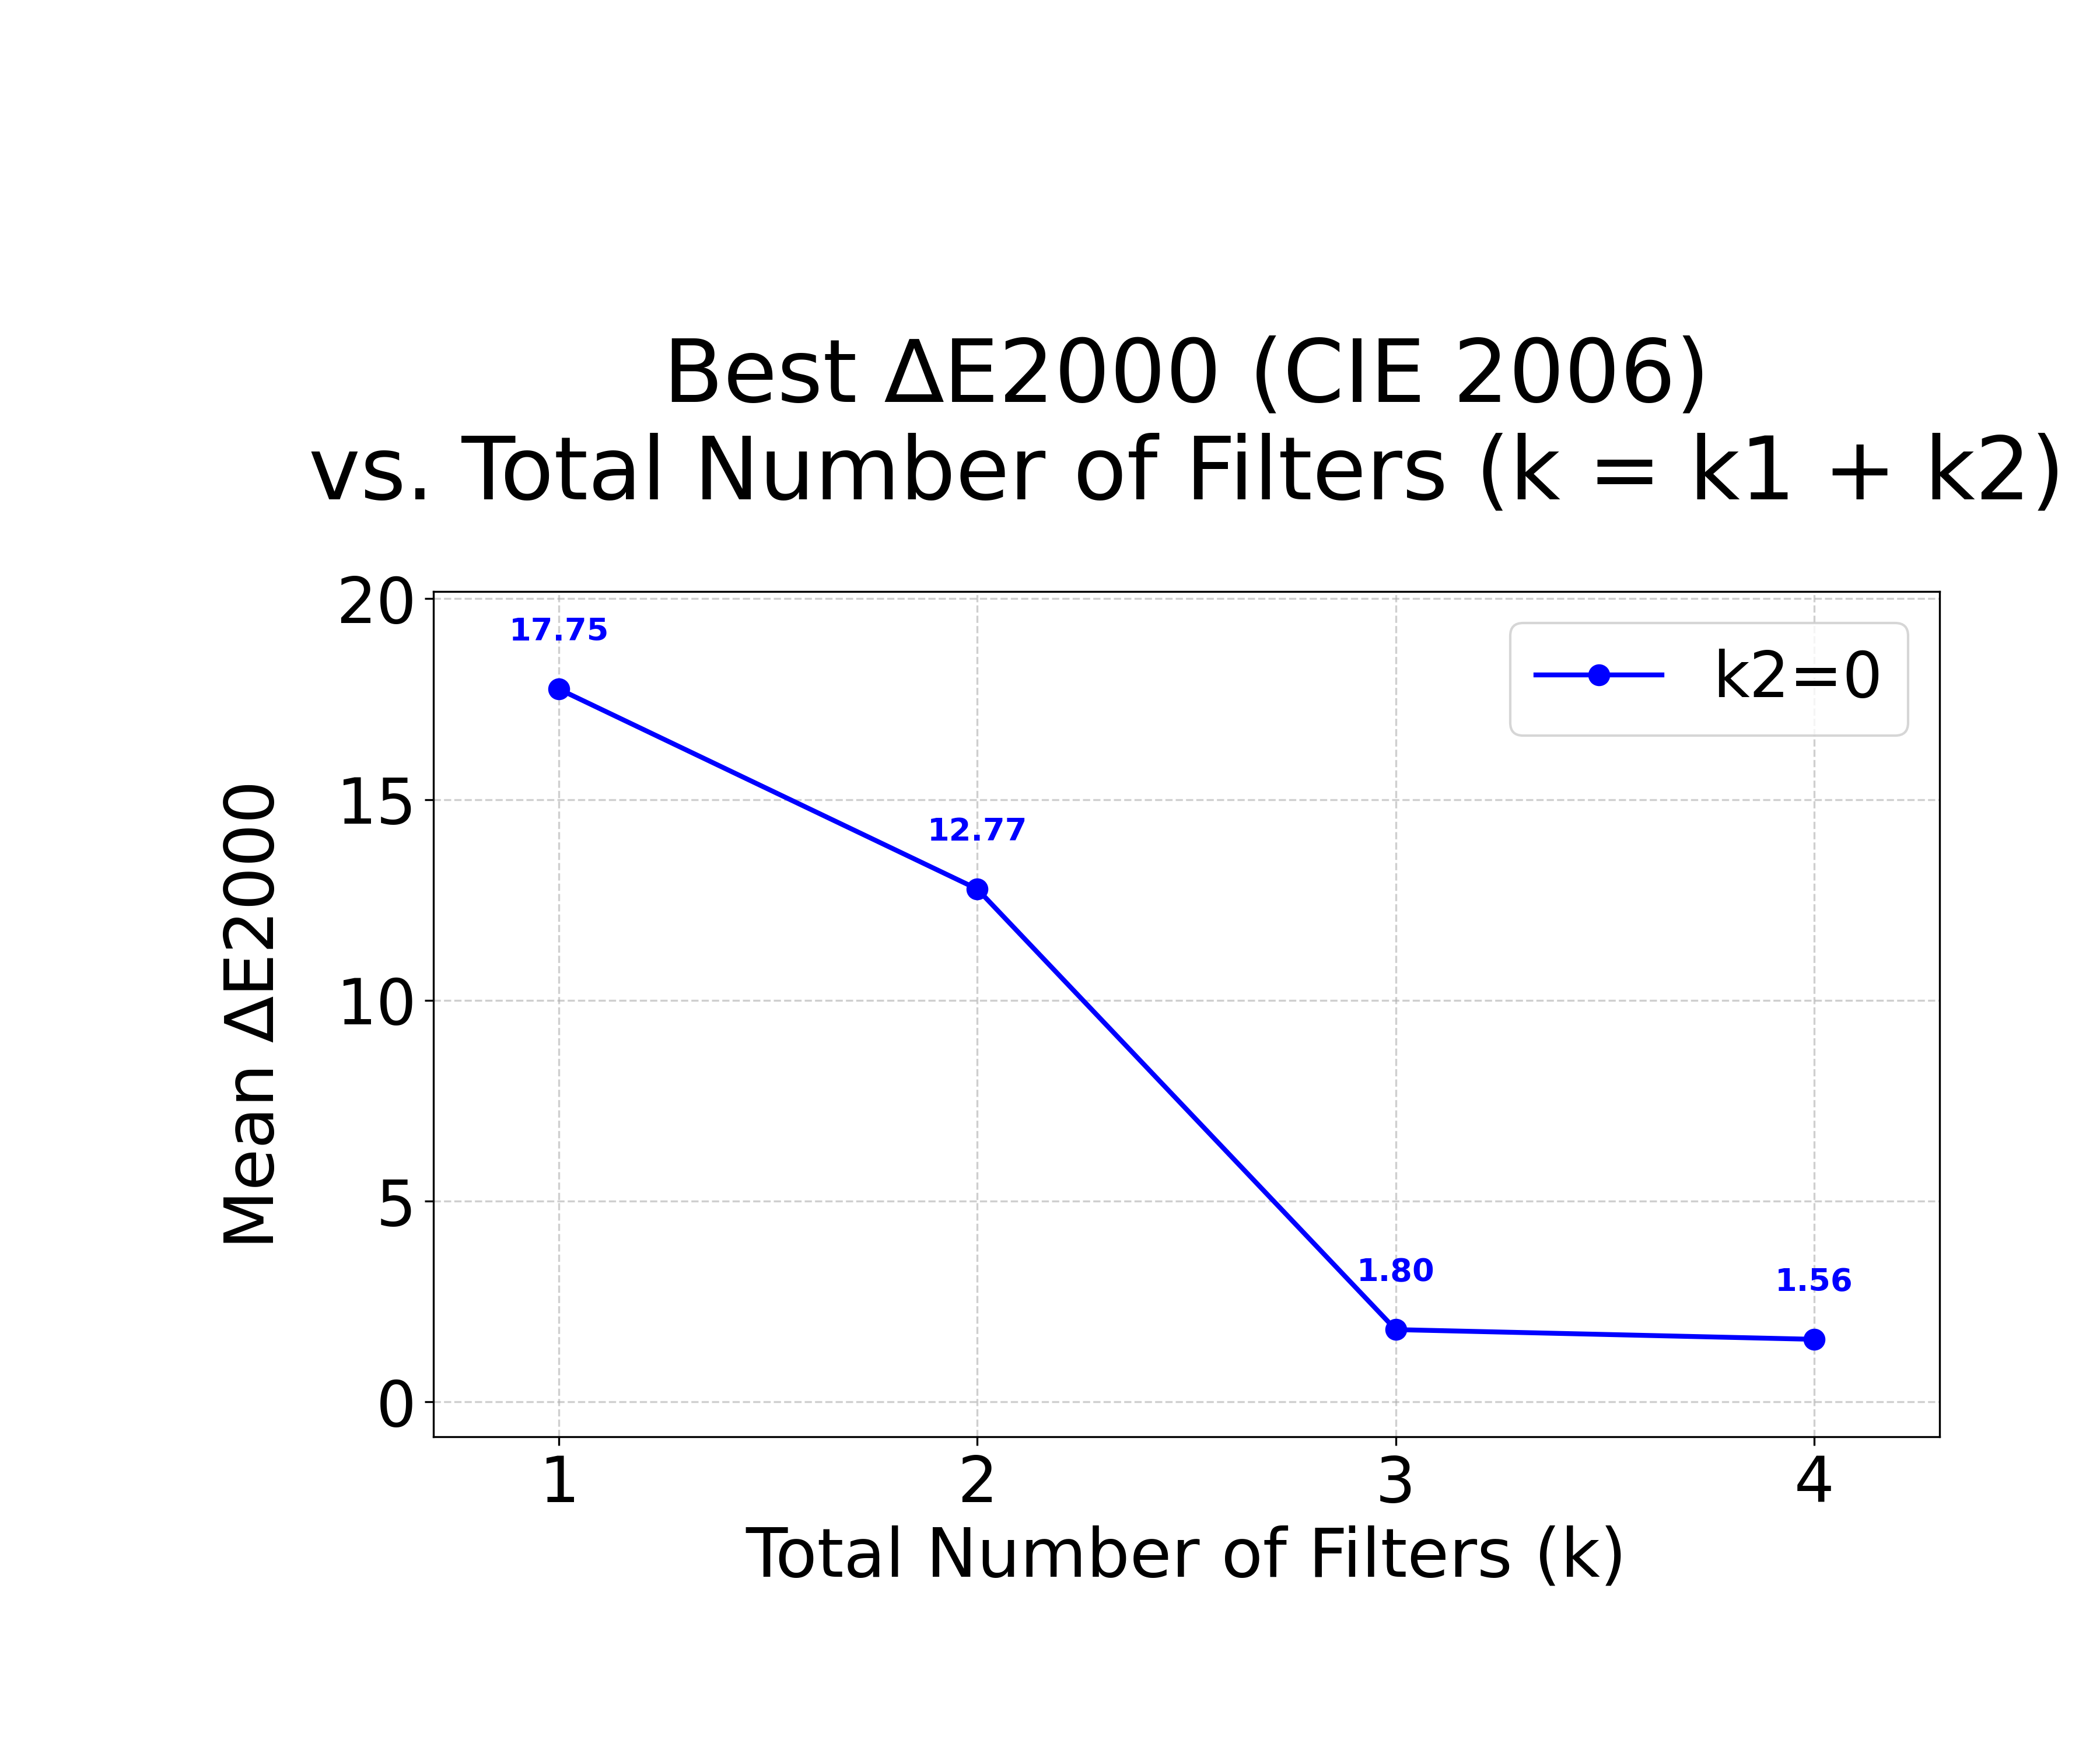
\includegraphics[width=\linewidth]{media/scraped_k4_nDeltaEChart.png}
    \caption{Mean $\dE$ of best combination for each number of scraped filters $k < 5$}
\end{subfigure}%
\begin{subfigure}{.49\linewidth}
    \centering
    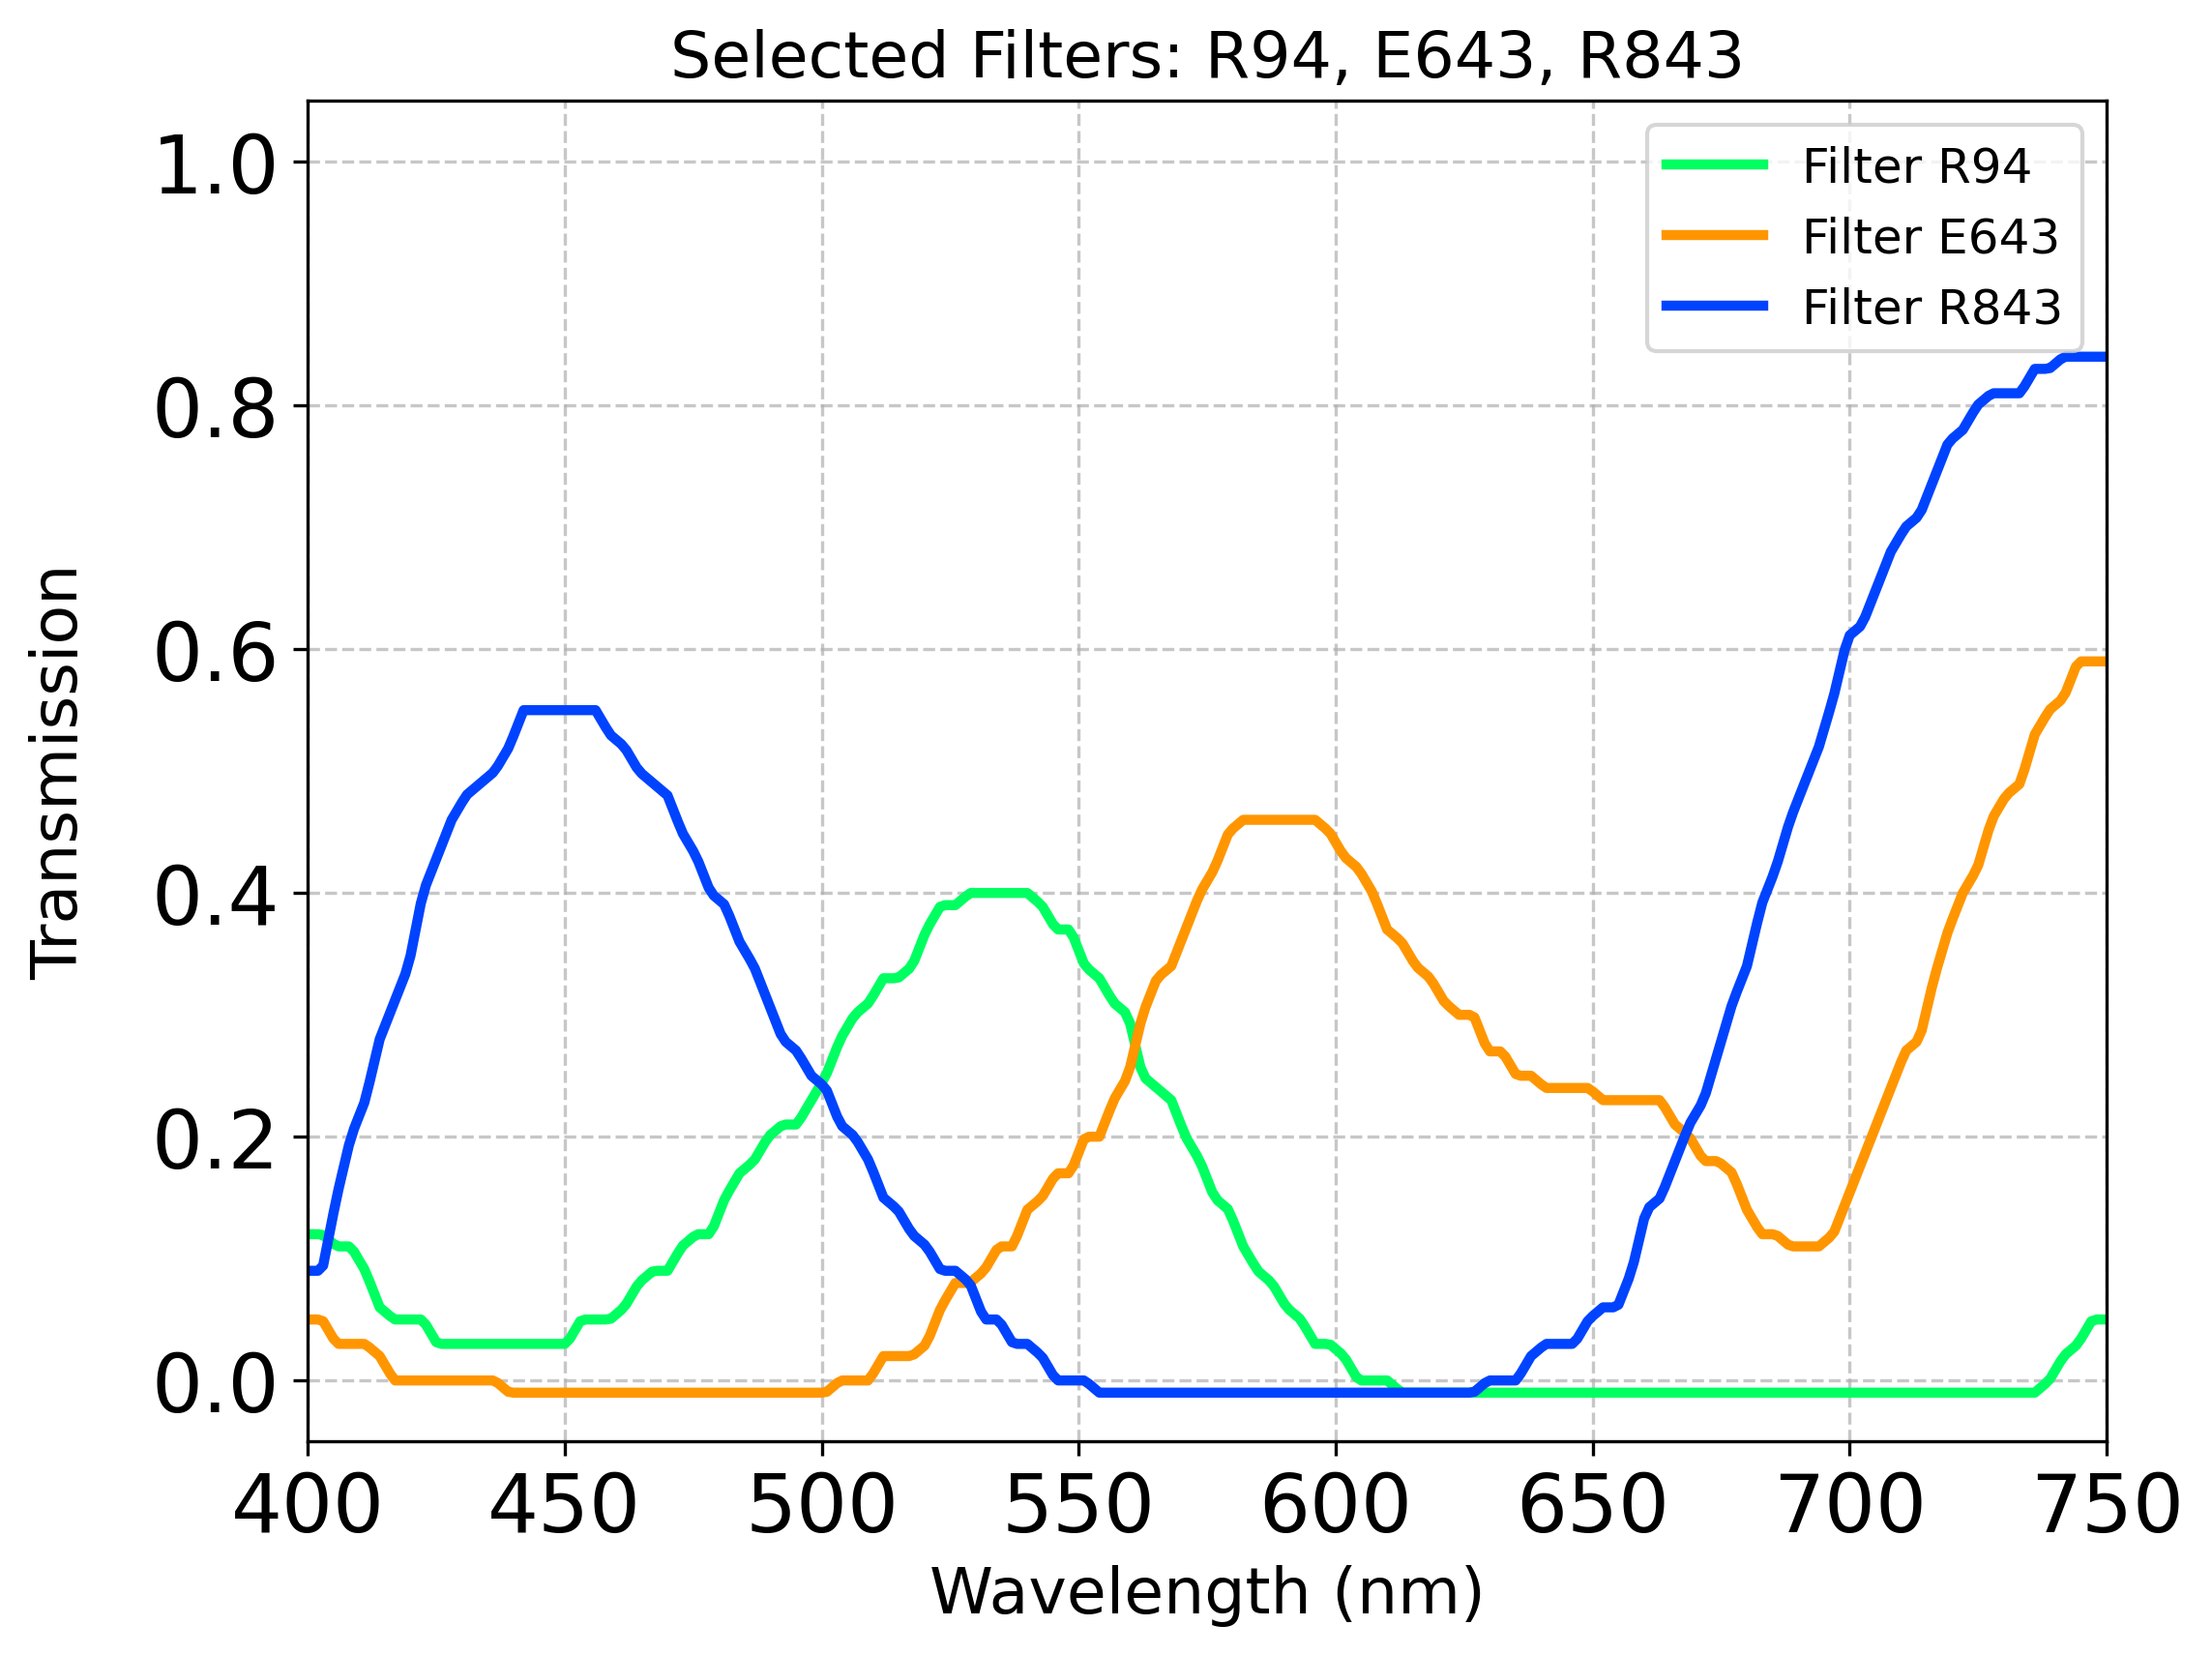
\includegraphics[width=\linewidth]{media/scraped_k3_front_page_right.png}
    \caption{Transmission functions for optimal MyColor $k=3$ solution}
\end{subfigure}
\caption{MyColor $k<5$ performance and selected filters.}
\end{figure}

Indeed, we can visually inspect the transmission functions above to see that our functions share approximate modes with the XYZ functions, given that the right tails will be neutralized above 650nm by the presence of our IR-cut filter.

Their transformations after multiplication by $\boldsymbol{M}$ are shown below, including a simulated IR-cut filter which cuts off most transmission above 650nm.
These are overlaid on the CIE 2006 XYZ (from LMS) functions.

\begin{figure}[H]
\centering
\begin{subfigure}{.55\linewidth}
    \centering
    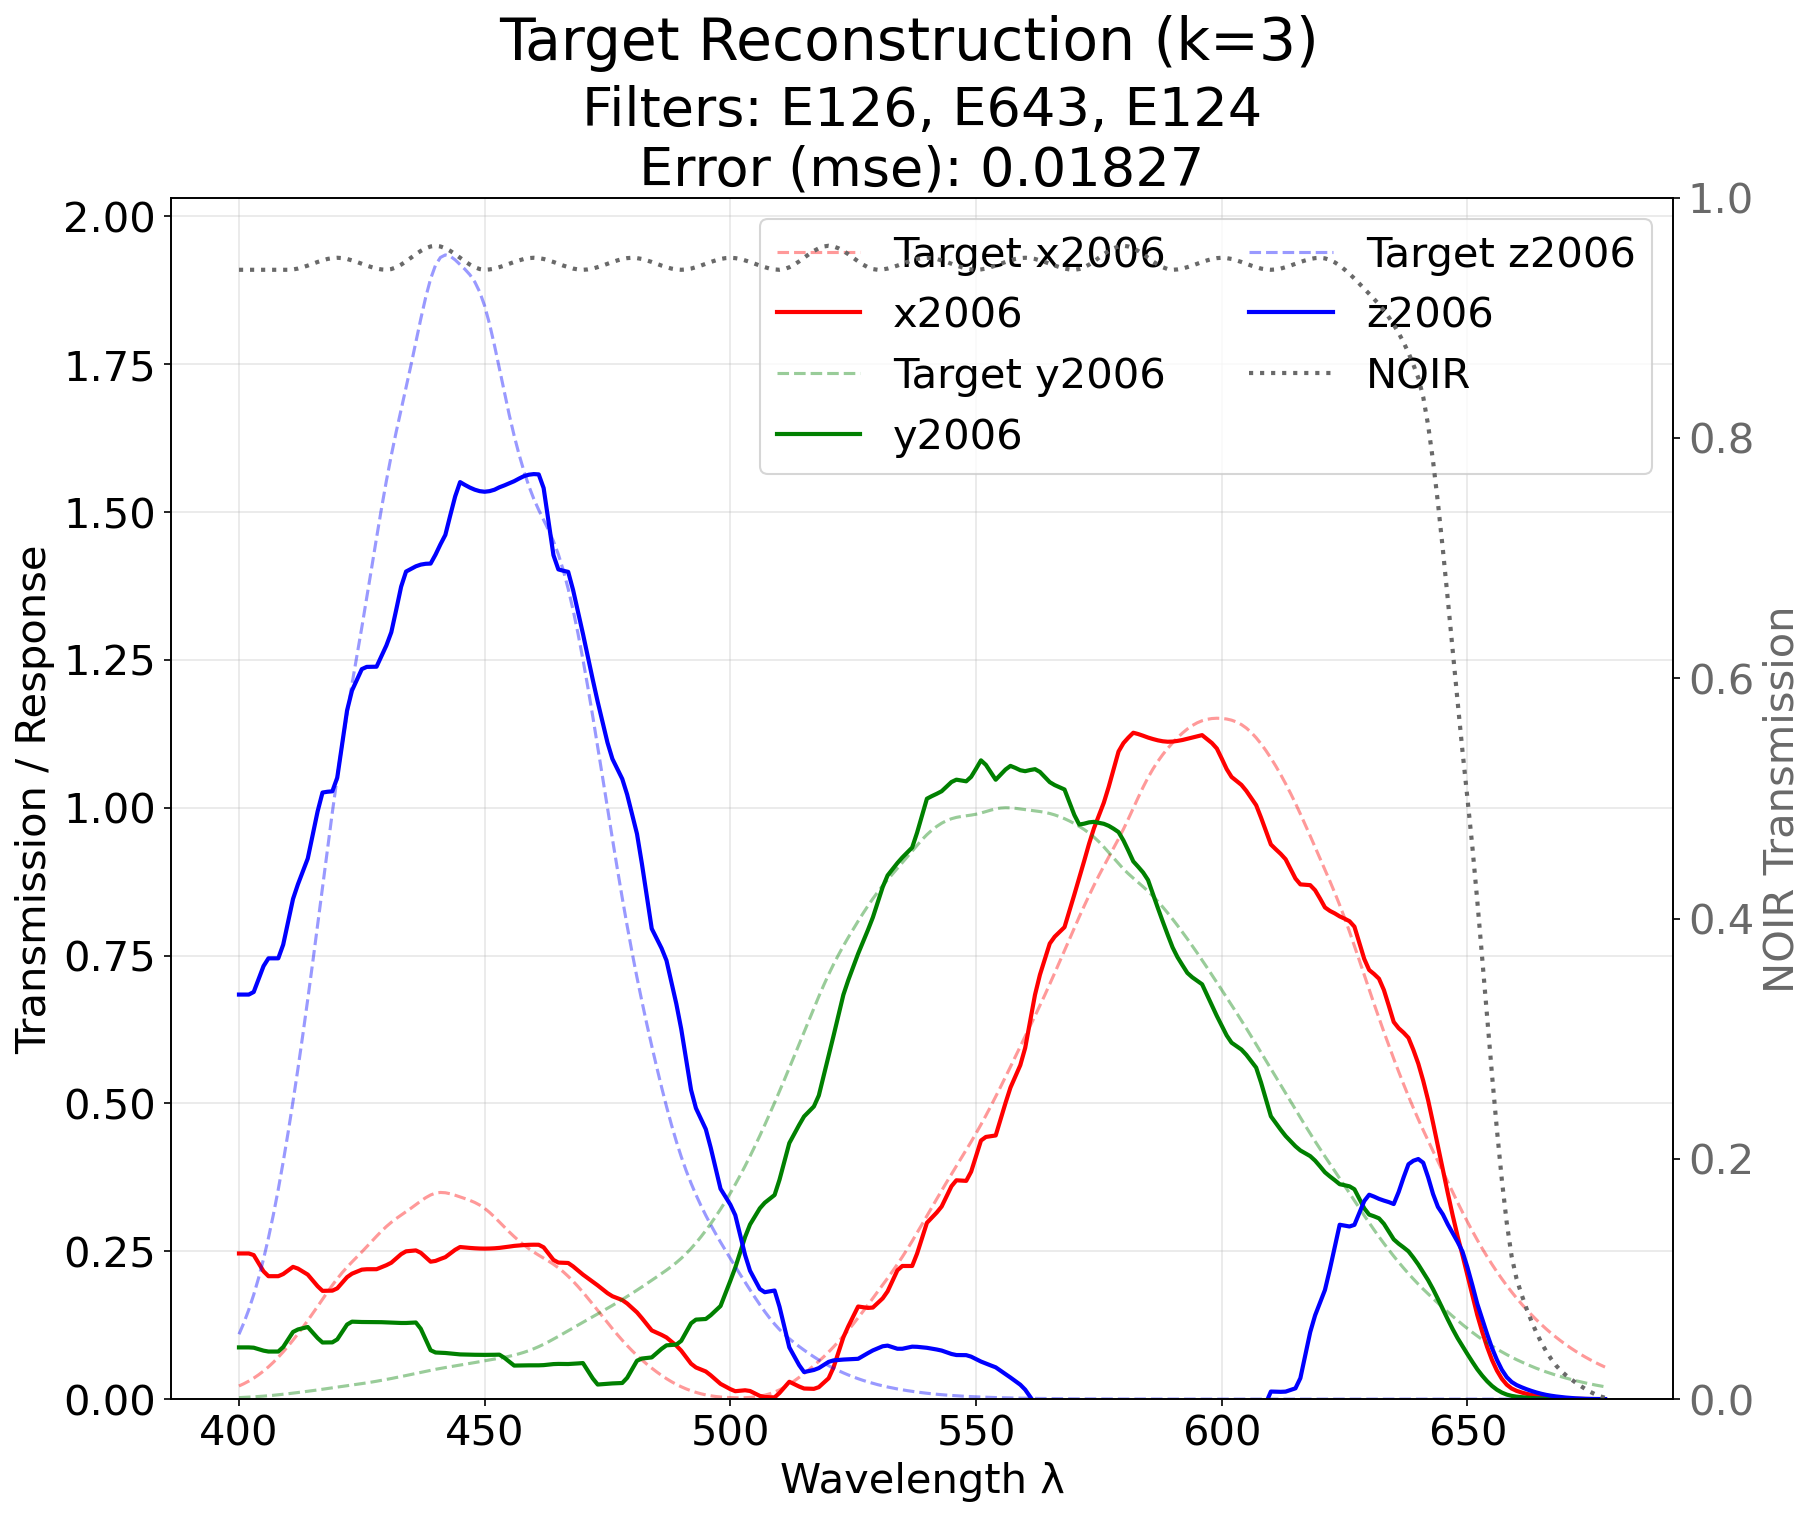
\includegraphics[width=\linewidth]{media/scraped_k3_spectra.png}
    \caption{Transformed transmission functions with CIE 2006 XYZ spectral response functions}
\end{subfigure}%
\begin{subfigure}{.44\linewidth}
    \centering
    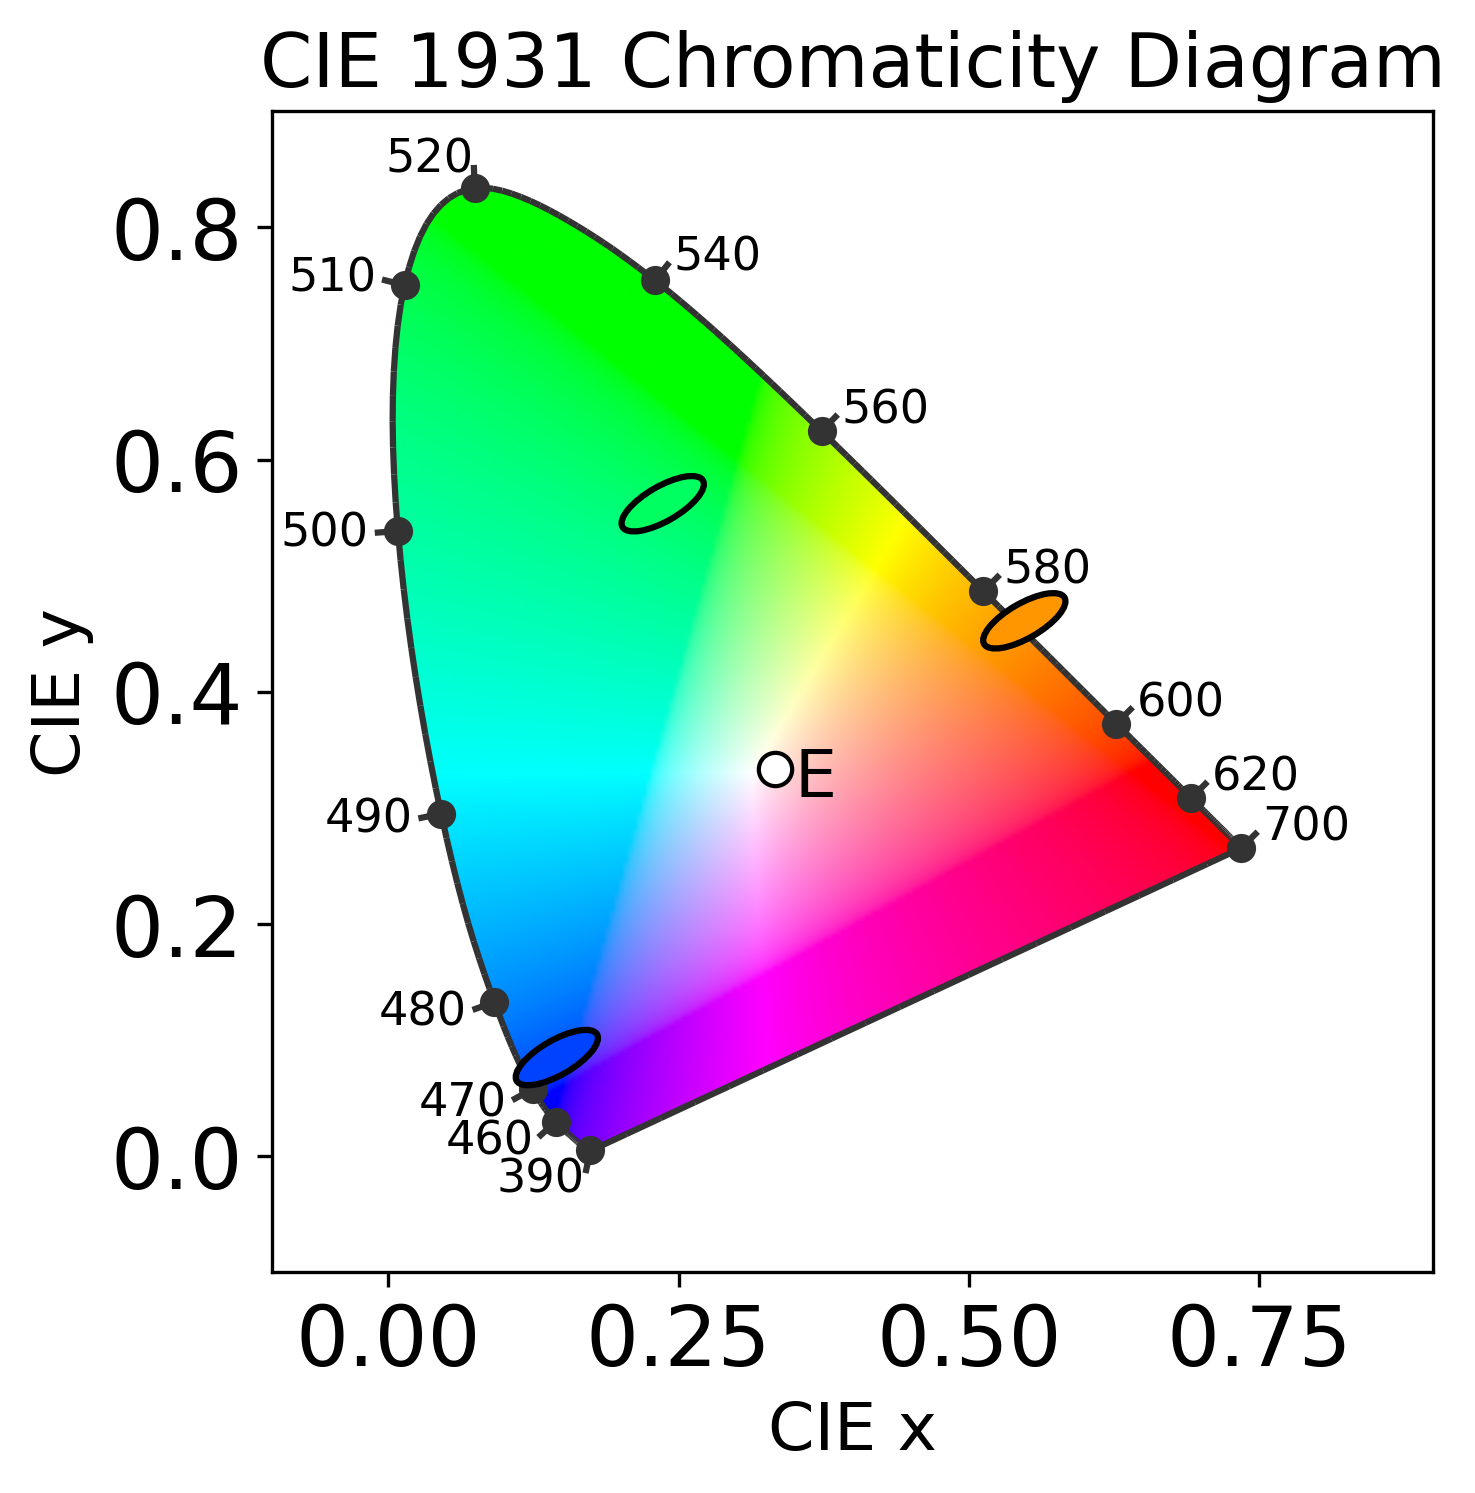
\includegraphics[width=\linewidth]{media/scraped_gamut_k3.png}
    \caption{Best filters from MyColor at $k=3$ on the color gamut}
\end{subfigure}
\caption{MyColor $k=3$ filters in spectral and chromaticity space.}
\end{figure}

Additionally, we can view the filters' dominant wavelength overlaid onto the CIE 1931 Chromaticity Diagram in CIE x and CIE y space to see that these filters 'span' the entire gamut, and hence a linear combination of these filters may effectively reproduce any color on the gamut.
While we primarily utilize the New CIE 2006 LMS functions and their respective XYZ transformations (denoted CIE 2006), a significant body of research exists referring to the 1931 XYZ functions which provide helpful benchmarks for our performance. 
Further, the CIE 1931 Color Gamut diagram provides a natural and familiar demonstration of color within the CIE x and CIE y coordinates.  

More rigorous analysis requires the use of $\dE$ calculations using a color checker, and in this case, our mean $\dE$ across 24 patches reached the value of 1.80.

\begin{figure}[H]
\centering
\begin{subfigure}{.4\linewidth}
    \centering
    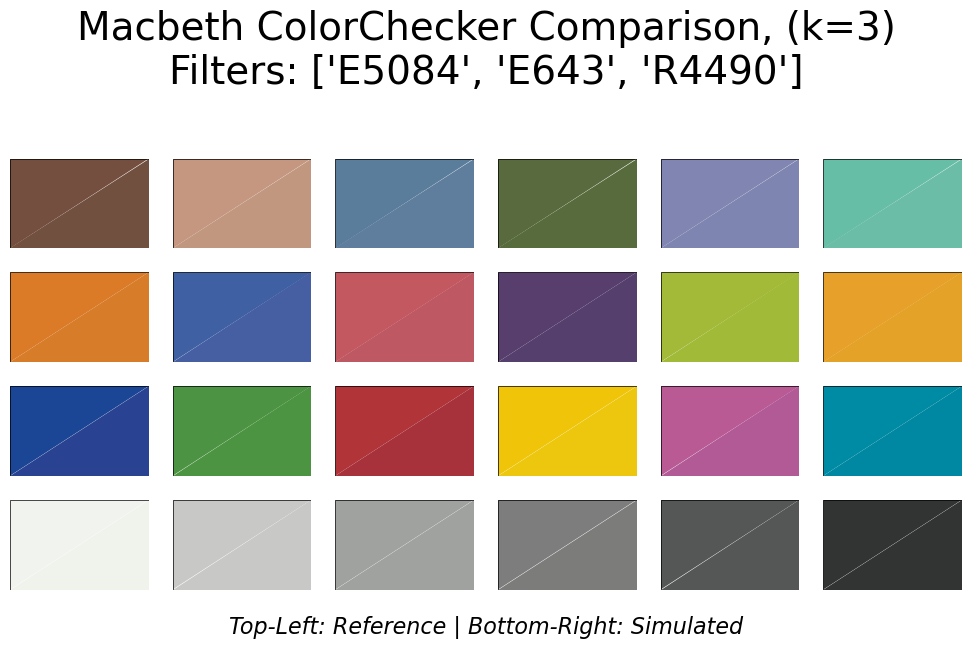
\includegraphics[width=\linewidth]{media/scraped_k3_macbeth.png}
    \caption{Macbeth Color Checker for $k=3$ with MyColor filters}
\end{subfigure}%
\begin{subfigure}{.45\linewidth}
    \centering
    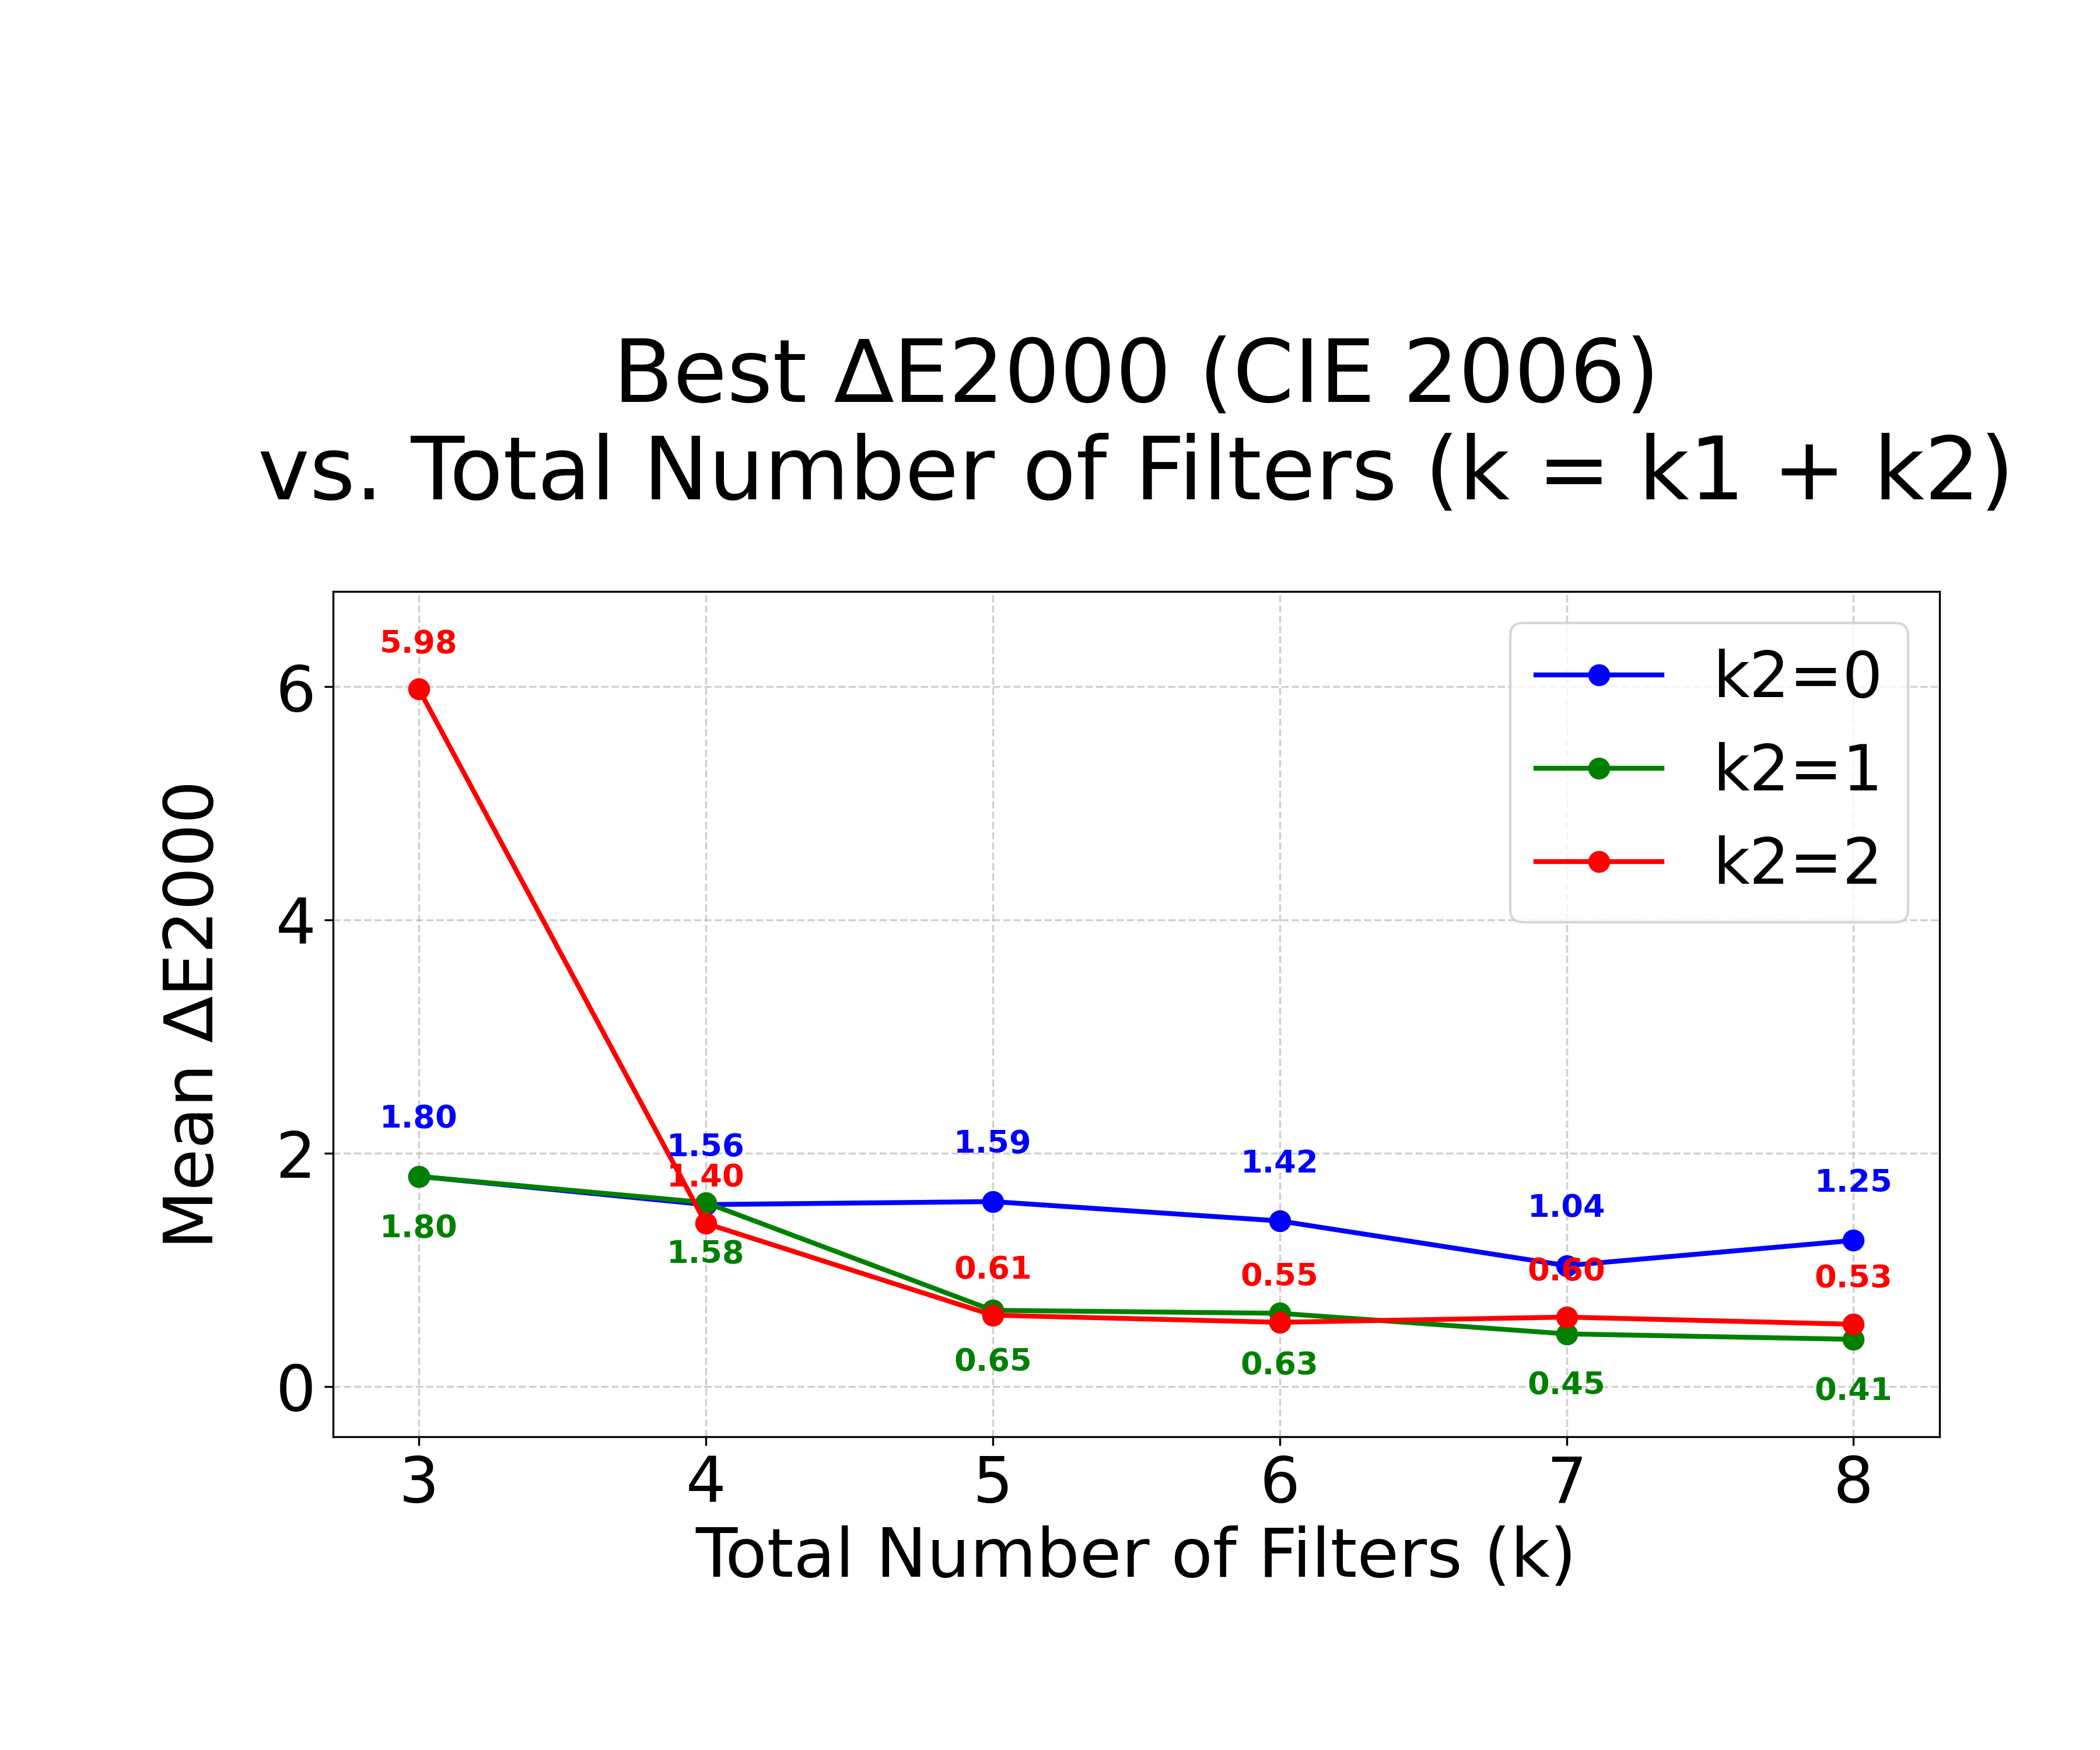
\includegraphics[width=\linewidth]{media/scraped_k1scaled_deltaE.png}
    \caption{$\dE$ for $k \in \{3...8\}$ and $k_1 \in \{0,1,2\}$}
\end{subfigure}
\caption{MyColor evaluation on a color checker and scaling to larger $k$.}
\end{figure}

While $\dE$ of 1.80 is sufficient for human-centered applications in controlled lighting, we can improve upon this result and strive for lower MSE results.
With the full set of 494 filters, we are unable to compute a brute-force solution in reasonable time, and must utilize heuristic solutions.
Fortunately, the heuristic solutions augmented with a few brute force rounds provide effective solutions. 
We show up to $k=8$ filters' $\dE$ progressions as a function of $k$ above. 

This result supports our intuition that we can achieve $\dE$ values comparable with state of the art results using our analysis.
Importantly, the improvement in $\dE$ largely flattens after $k=5$, providing useful knowledge as to the necessary number of filters to attain a high-quality reconstruction.
We include a rendering from the CAVE dataset reconstructed with the $k=5 (k_1=4,k_2=1)$ solution for an example of a practical simulated filter wheel setup. 
We also provide the $k=2 (k_1=2,k_2=0), \dE=12.77$ solution for comparison.  

\begin{figure}[H]
\centering
\begin{subfigure}{.49\linewidth}
    \centering
    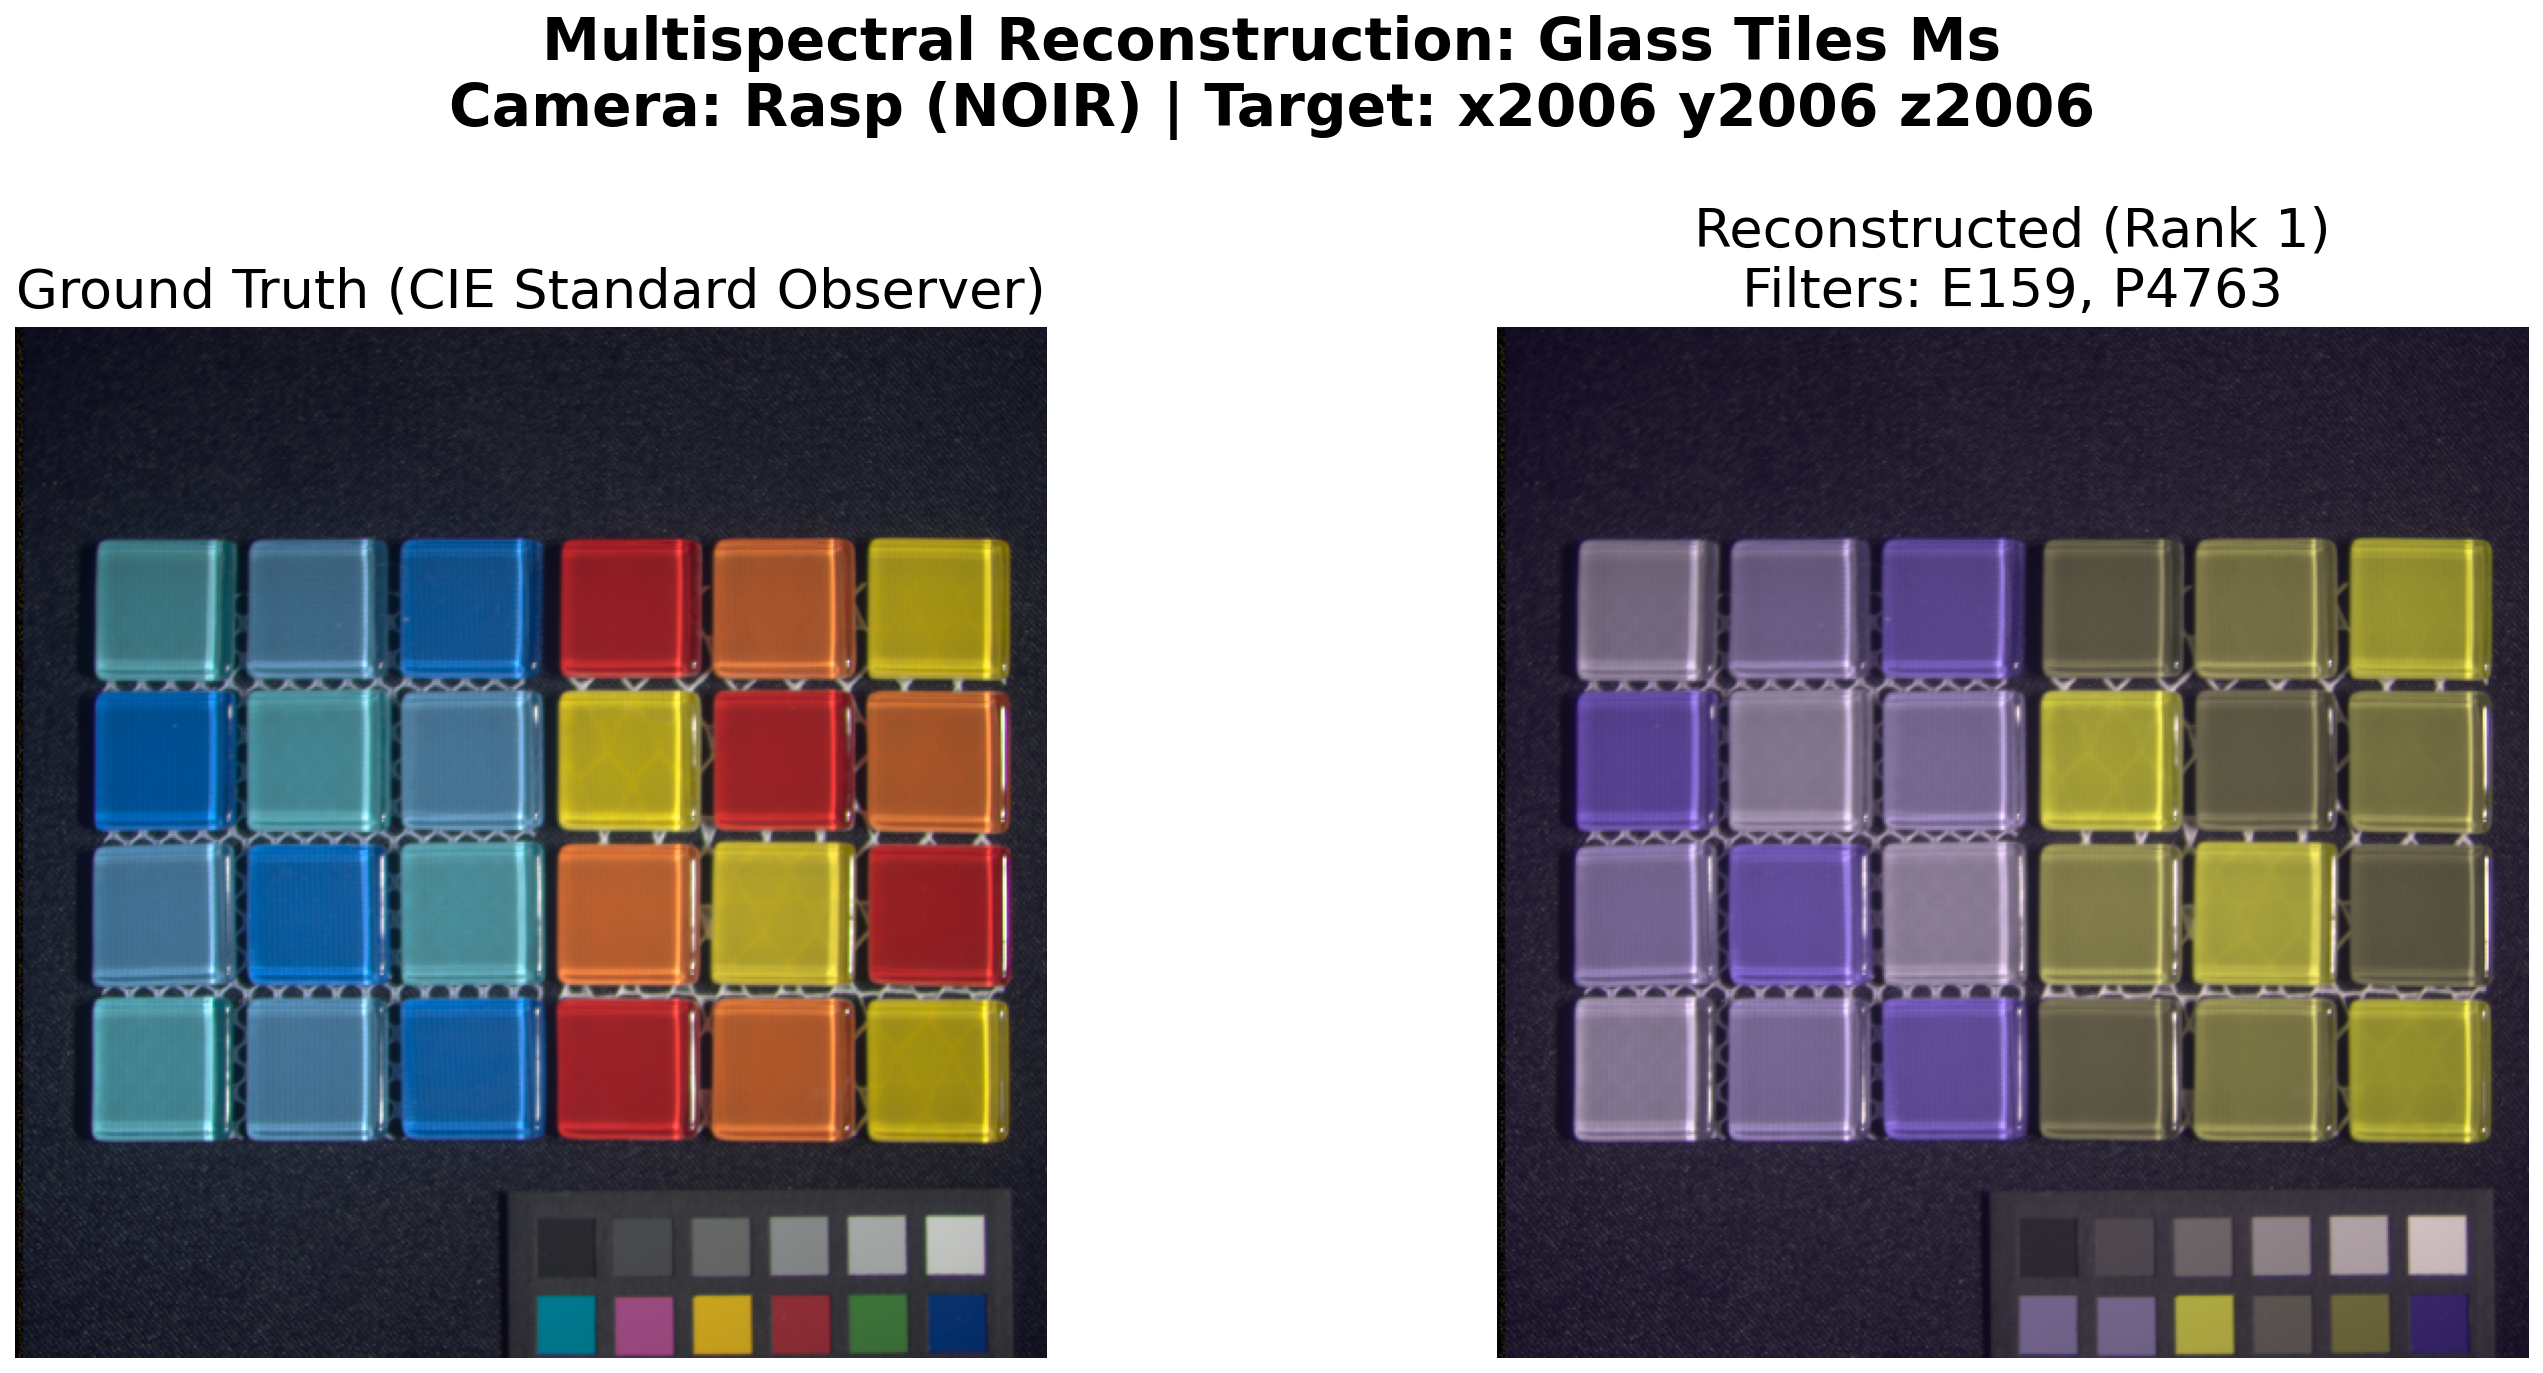
\includegraphics[width=\linewidth]{media/scraped_tiles_cave_k2.png}
    \caption{CAVE 'glass tiles' scene with scraped filters, $k=2 (k_1=2,k_2=0)$}
\end{subfigure}%
\begin{subfigure}{.49\linewidth}
    \centering
    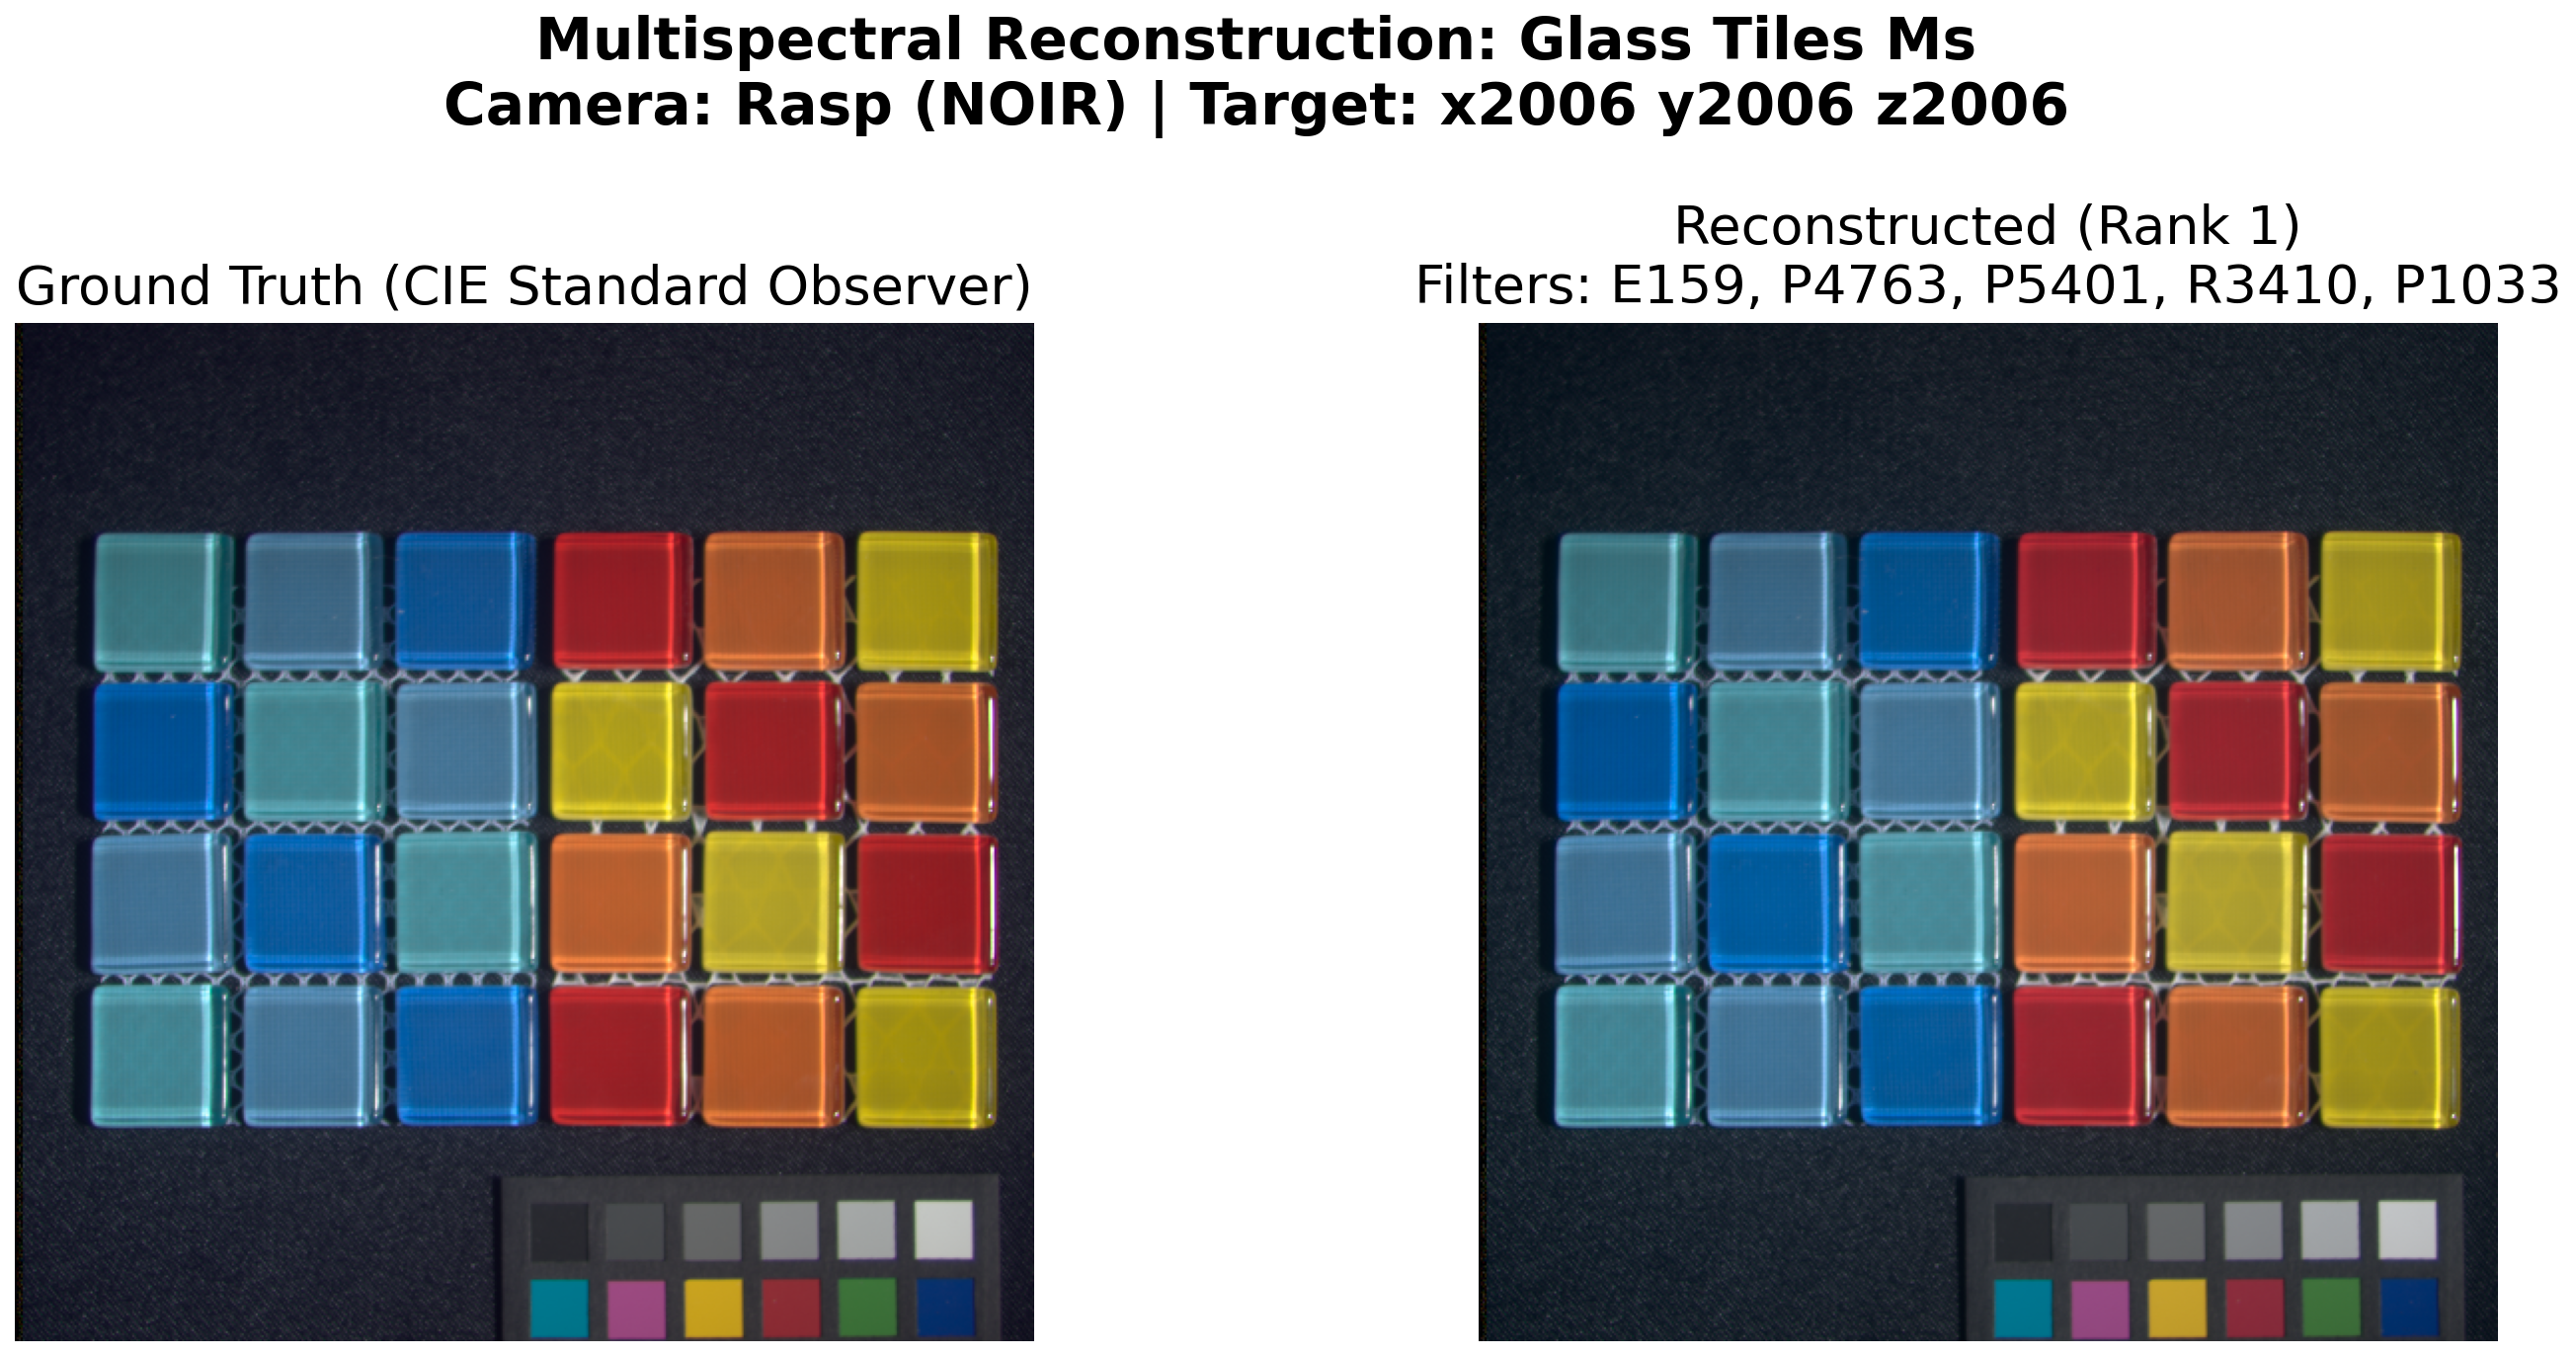
\includegraphics[width=\linewidth]{media/scraped_tiles_cave_k5.png}
    \caption{CAVE 'glass tiles' scene with scraped filters $k=5 (k_1=4,k_2=1)$}
\end{subfigure}
\caption{Comparison of different CAVE renders with scraped filters}
\end{figure}

We note that the set of 494 filters provides a large candidate pool, making it comparatively easy to reconstruct the desired target functions, subject to our ability to correctly identify a good combination. 
In the next section, we explore a similar analysis on a smaller set of filters, searching for an equivalent reconstruction quality and more easily calculating the performance difference against the best possible solution as found by brute force, which we cannot feasibly compute for the $N=494$ sized set of filters. 

\section{Rosco Supergel Set in Simulated Camera}

In this section, we progressively increase the number of filters $k$ and analyze the reconstruction quality for each. 
We comment on the increases in reconstruction quality afforded by each incremental extra capture, understanding that each filter increases capture time and possibility of a 'bad capture.'
Specifically, because  we require a mechanical servo turn between each capture, if an object in our scene moves, or worse, if our camera moves during capture, our reconstruction will be irrecoverably damaged. 

To maintain consistency across this demonstration, we run all the simulations in the following section with an IR-cut filter included. 
Additionally, for the computations of $\dE$, we utilize the python \codeword{color} and \codeword{colour-science} libraries, with the CIE 1931 or 2015 2 Degree Standard Observer respectively, depending on whether we utilize the CIE 1931 or CIE 2006 XYZ functions. 
D65 illuminant from the same library is used as well as ColorChecker N Ohta reflectance patches. XYZ responses were converted to CIELAB using the \codeword{color.xyz2lab} function to convert XYZ signals to lab before $\dE$ computation.

\subsection{MSE, $\dE$ and CAVE Results for $k \in \{3,4,5\}$}

We will provide some filter wheel prescriptions along the various values of $k$ we consider for our filter wheel. 
In Figure \ref{fig:supergelIntro}, we show the best $\dE$ of our approximation at each $k$ filter subset of the Rosco Supergel set, where $k\in \{1,8\}$. 
For completeness and surety of optimal combination identification, we use brute force search in this section, thus $k=k_1$ and we omit $k_2$.
In this section, we continue to use the IR-cut filter and a standard MSE loss for consistency versus the prior section and other works. 

\begin{figure}[H]
\centering
\begin{subfigure}{.46\linewidth}
    \centering
    \includegraphics[width=\linewidth]{media/deltaE_vs_k_mse.png}
    \caption{Best $\dE$ for each number of filters $k$}
\end{subfigure}
\begin{subfigure}{.53\linewidth}
    \centering
    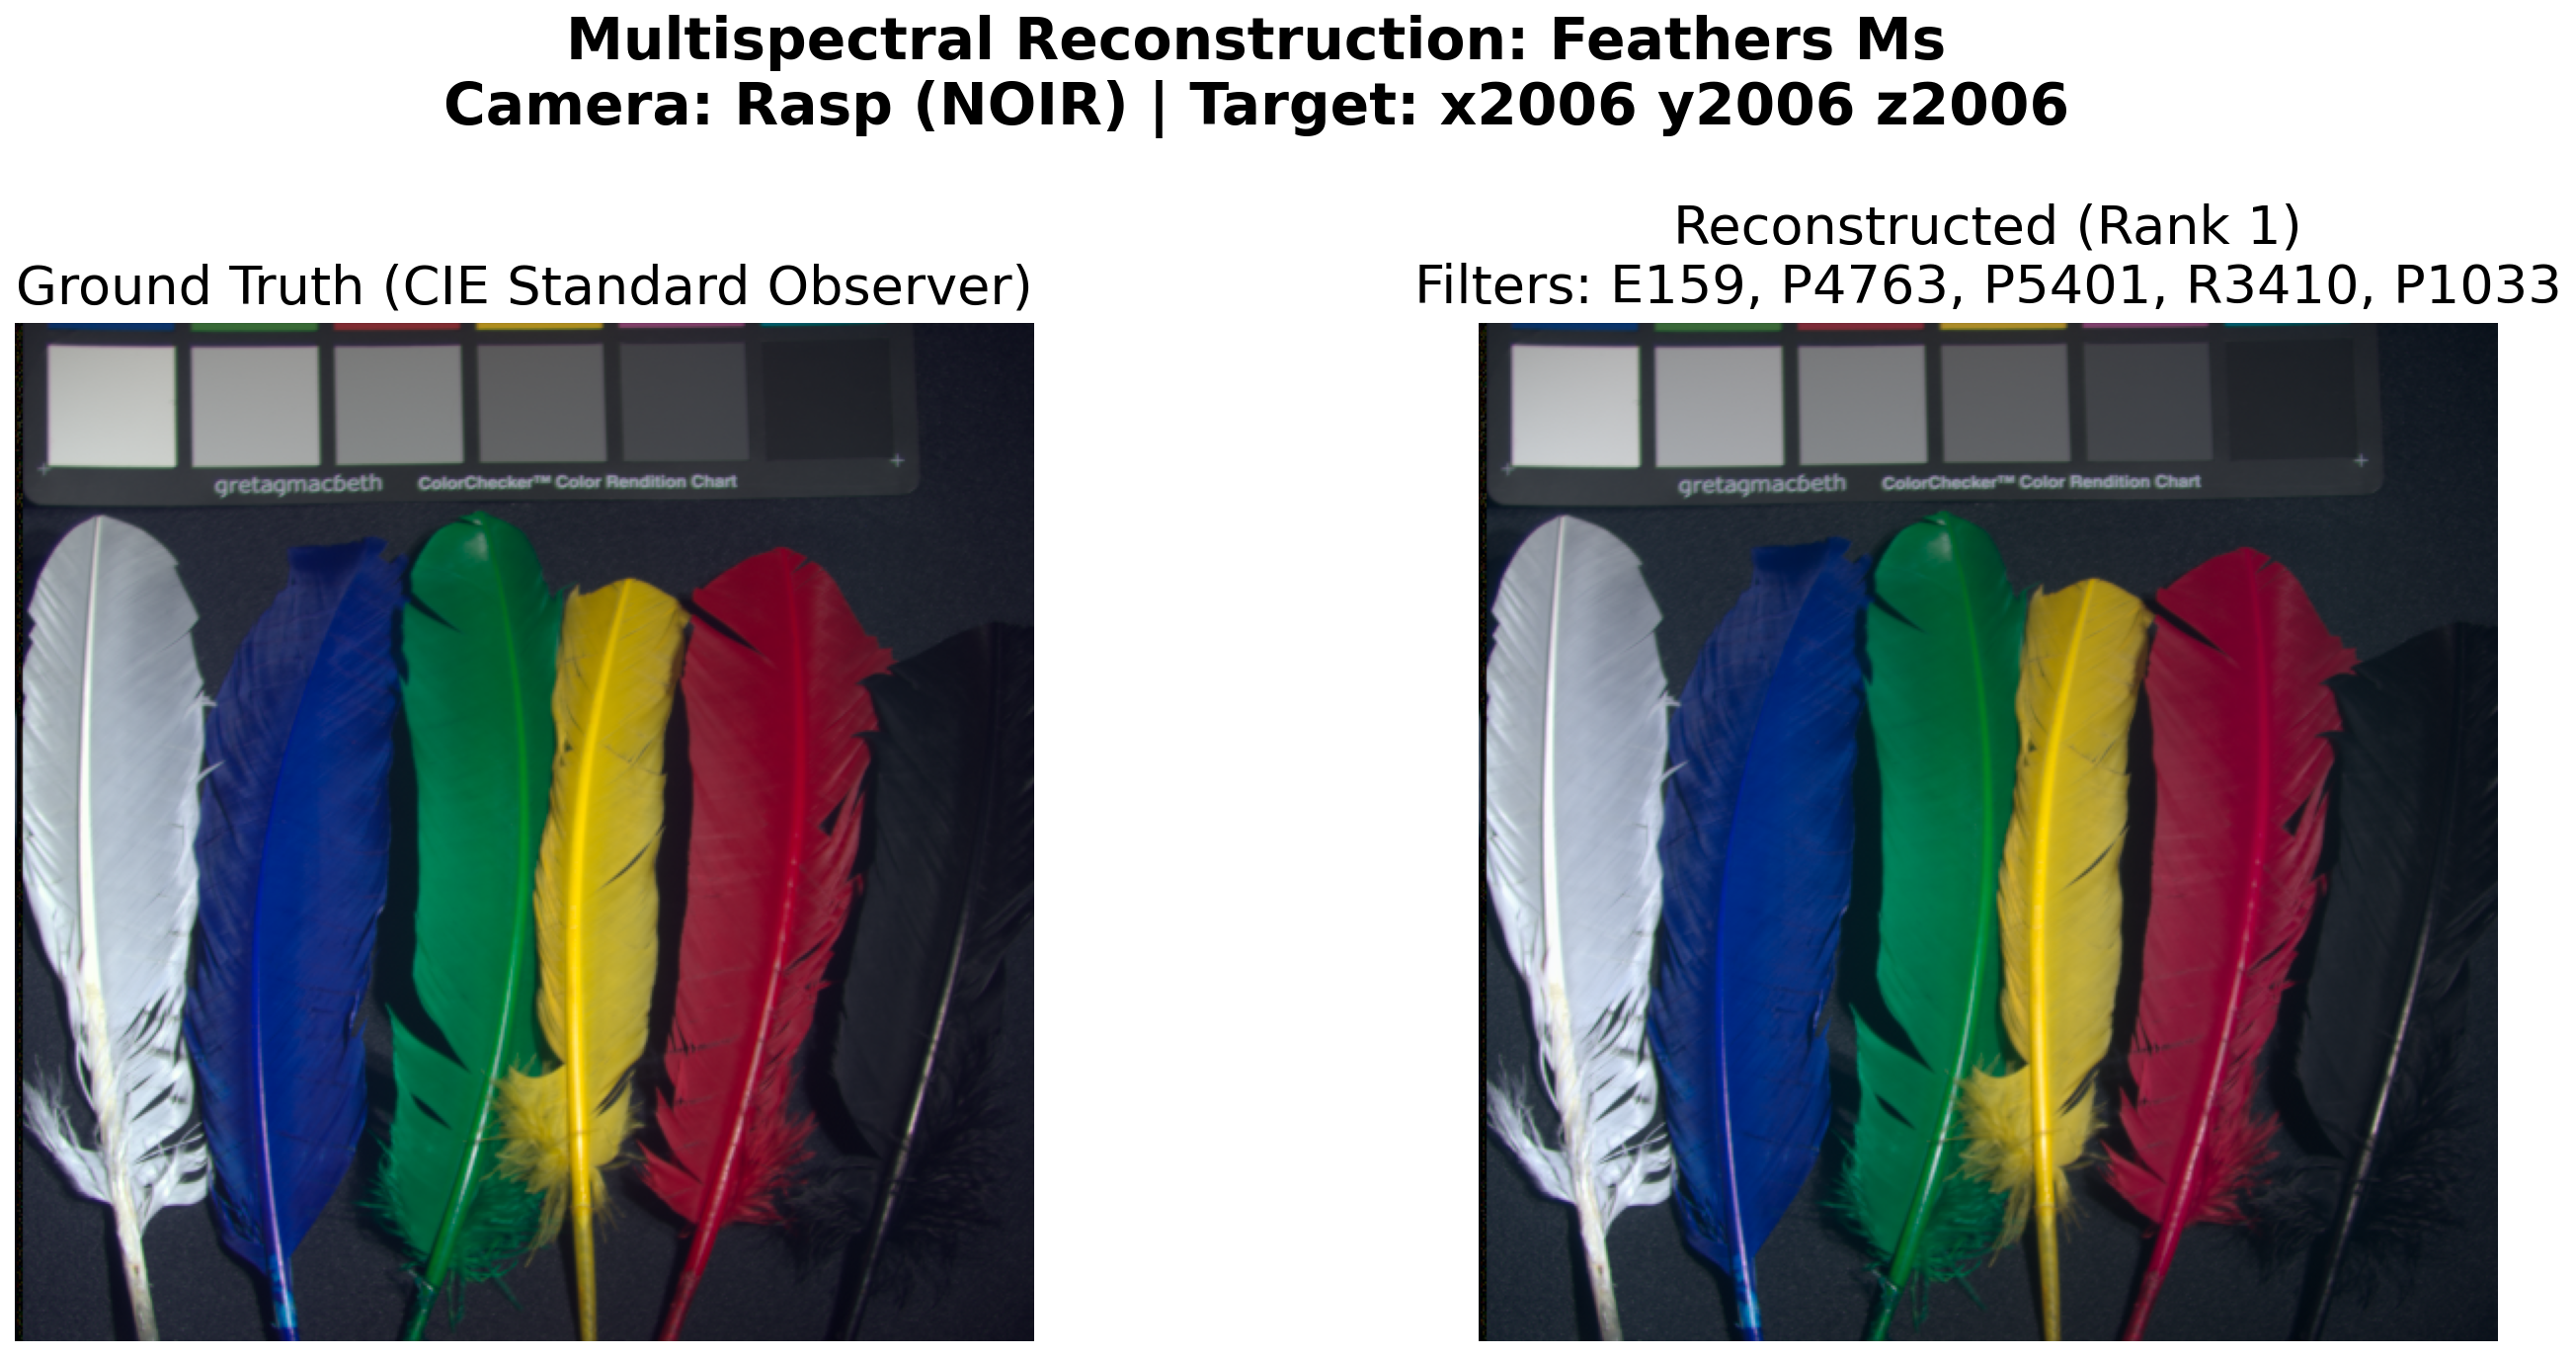
\includegraphics[width=\linewidth]{media/scraped_cave.png}
    \caption{CAVE rendering using best $k=5$ solution}
\end{subfigure}%
\caption{Example simulated reconstruction and overall Supergel set performance.}
\label{fig:supergelIntro}
\end{figure}

\subsubsection{Solution for $k=3$}

The best filter combination for $k=3$, clearly a poor spectral fit, see Fig. \ref{fig:k3spectral}, achieves a tolerable mean $\dE$ of 3.77. This is in the just noticeable difference threshold of 2-4 \cite{lindstrom2008delta},
indicating that the reconstructed colors may be distinguishable from the target colors under certain conditions. 
The 24 patches above show the original in the top left of each pane and the simulated reconstruction in the bottom right. It is evident there is a visible colour difference.
\begin{figure}[H]
\centering
\begin{subfigure}{.49\linewidth}
    \centering
    \includegraphics[width=\linewidth]{media/k3top1_spectra.png}
    \caption{Best XYZ reconstruction}
\end{subfigure}%
\begin{subfigure}{.49\linewidth}
    \centering
    \includegraphics[width=\linewidth]{media/n3MSEMacbeth.png}
    \caption{Macbeth Color Checker comparison}
\end{subfigure}
\begin{subfigure}{.49\linewidth}
    \centering
    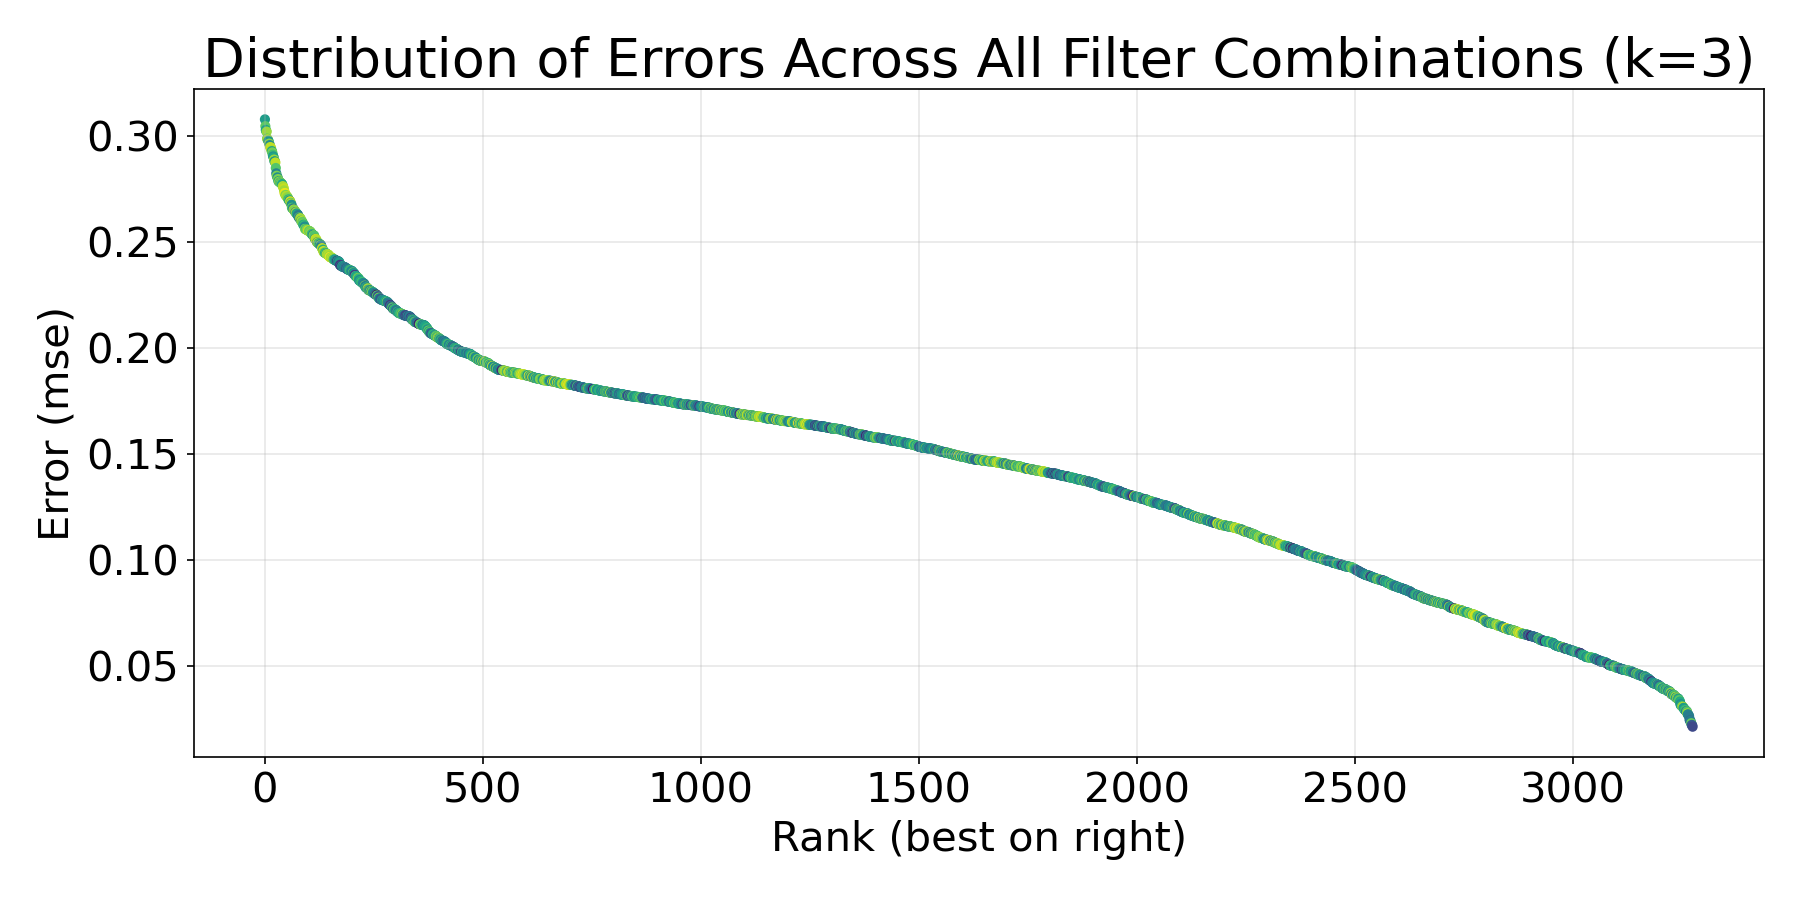
\includegraphics[width=\linewidth]{media/measured_k3_errors.png}
    \caption{Error distribution across combinations}
\end{subfigure}%
\begin{subfigure}{.49\linewidth}
    \centering
    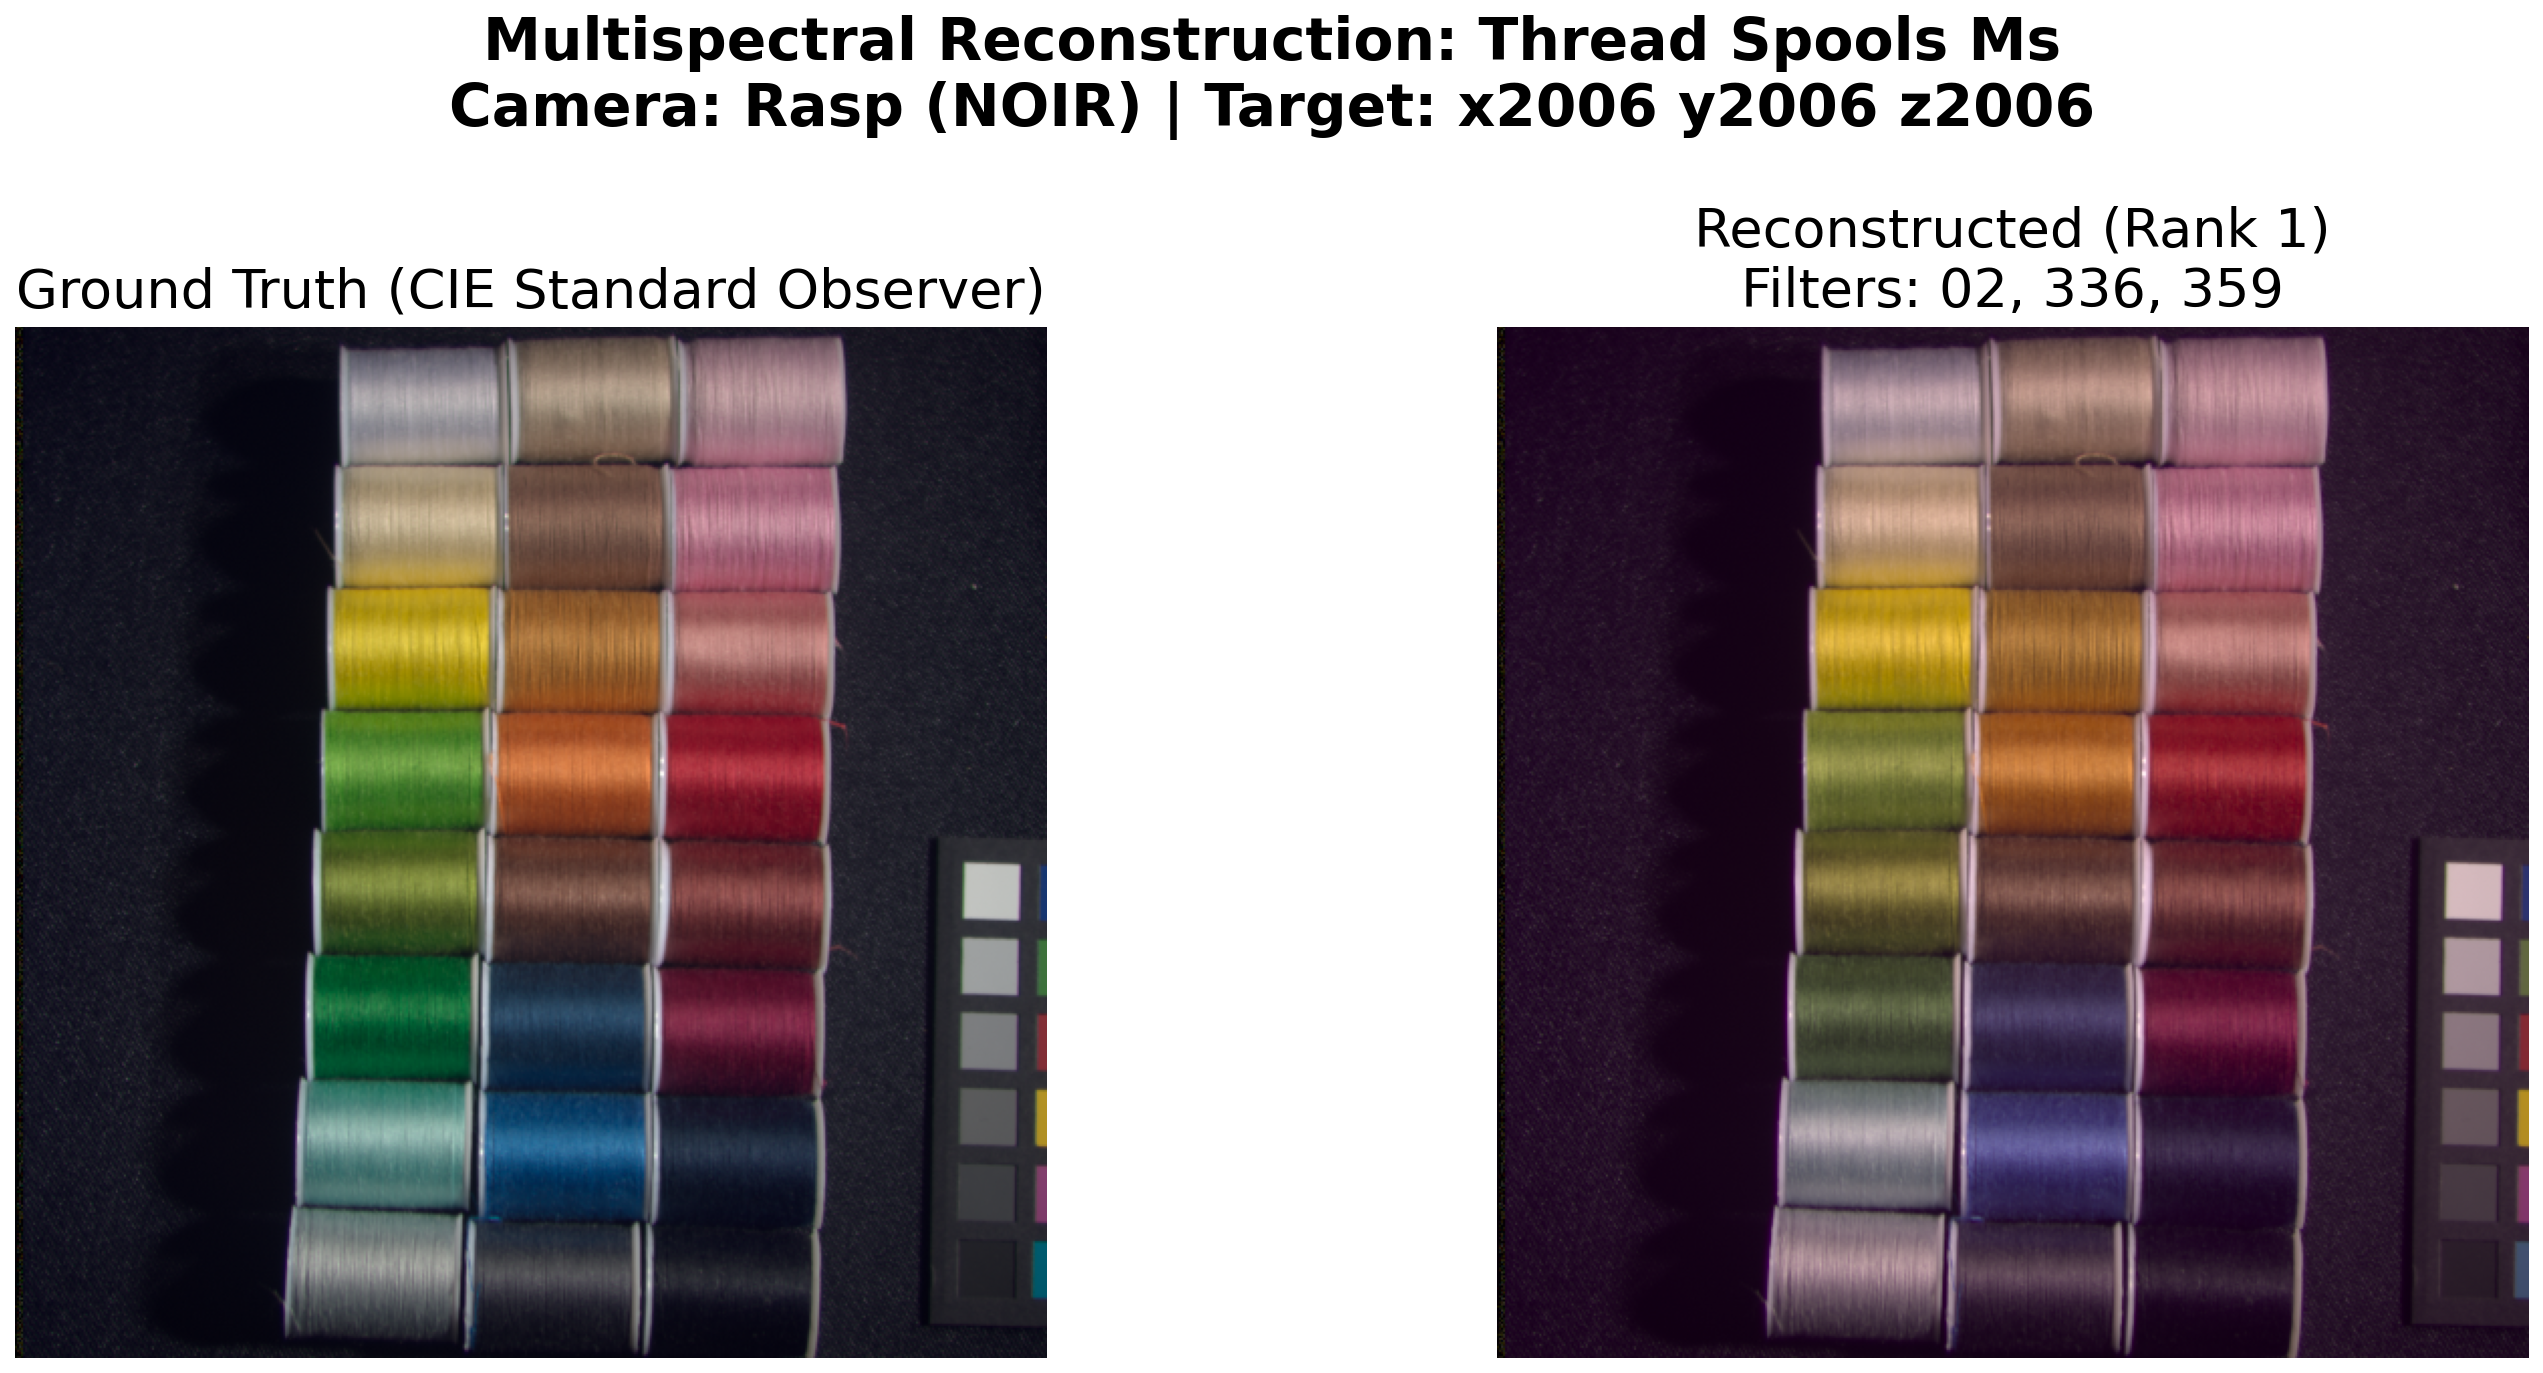
\includegraphics[width=\linewidth]{media/measured_k3_cave.png}
    \caption{CAVE render of combination}
\end{subfigure}
\caption{Supergel results for $k=3$.}
\label{fig:k3spectral}
\end{figure}

We also include some characteristics of the filters themselves, specifically the 1931 gamut locations and their measured transmission functions. 

\begin{figure}[H]
\centering
\begin{subfigure}{.40\linewidth}
    \centering
    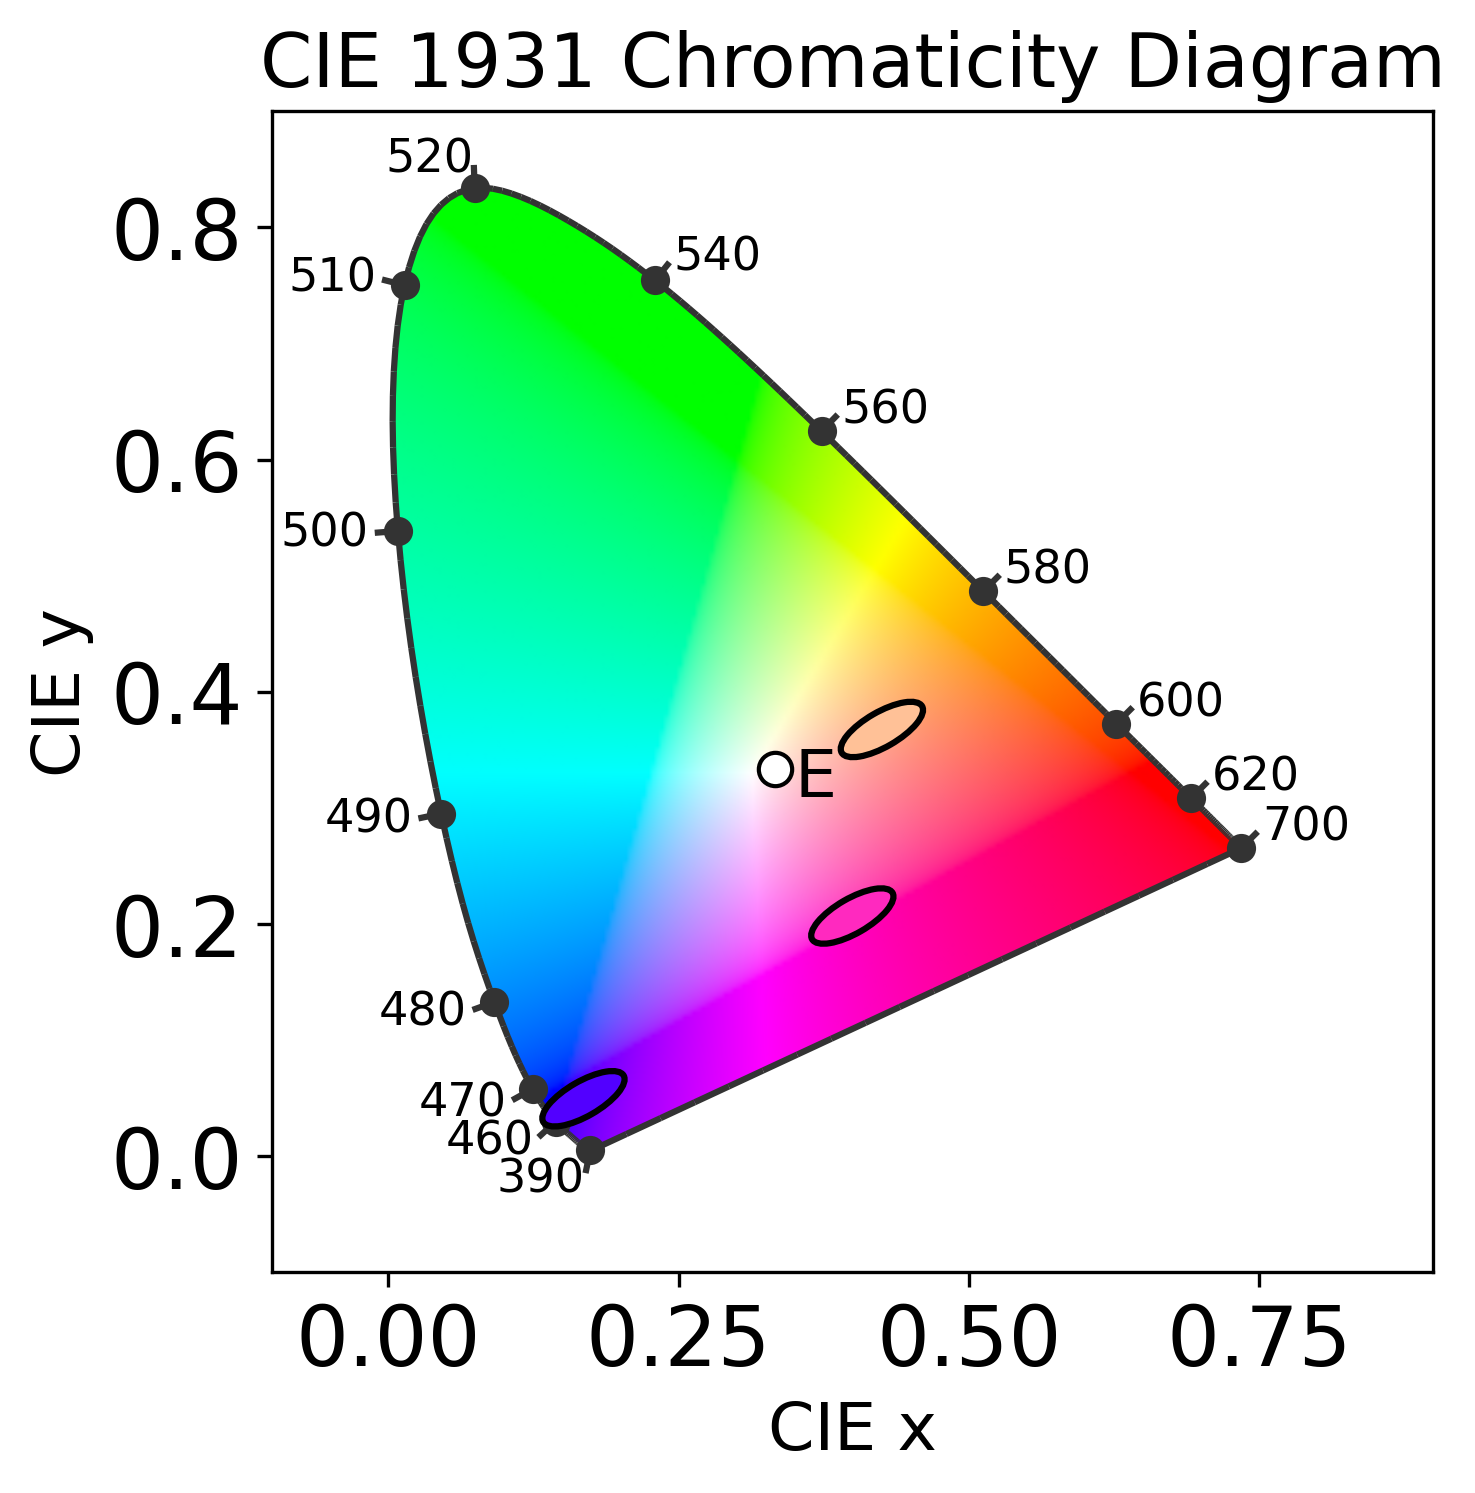
\includegraphics[width=\linewidth]{media/measured_k3_gamut.png}
    \caption{Location on CIE 1931 Color Gamut}
\end{subfigure}%
\begin{subfigure}{.55\linewidth}
    \centering
    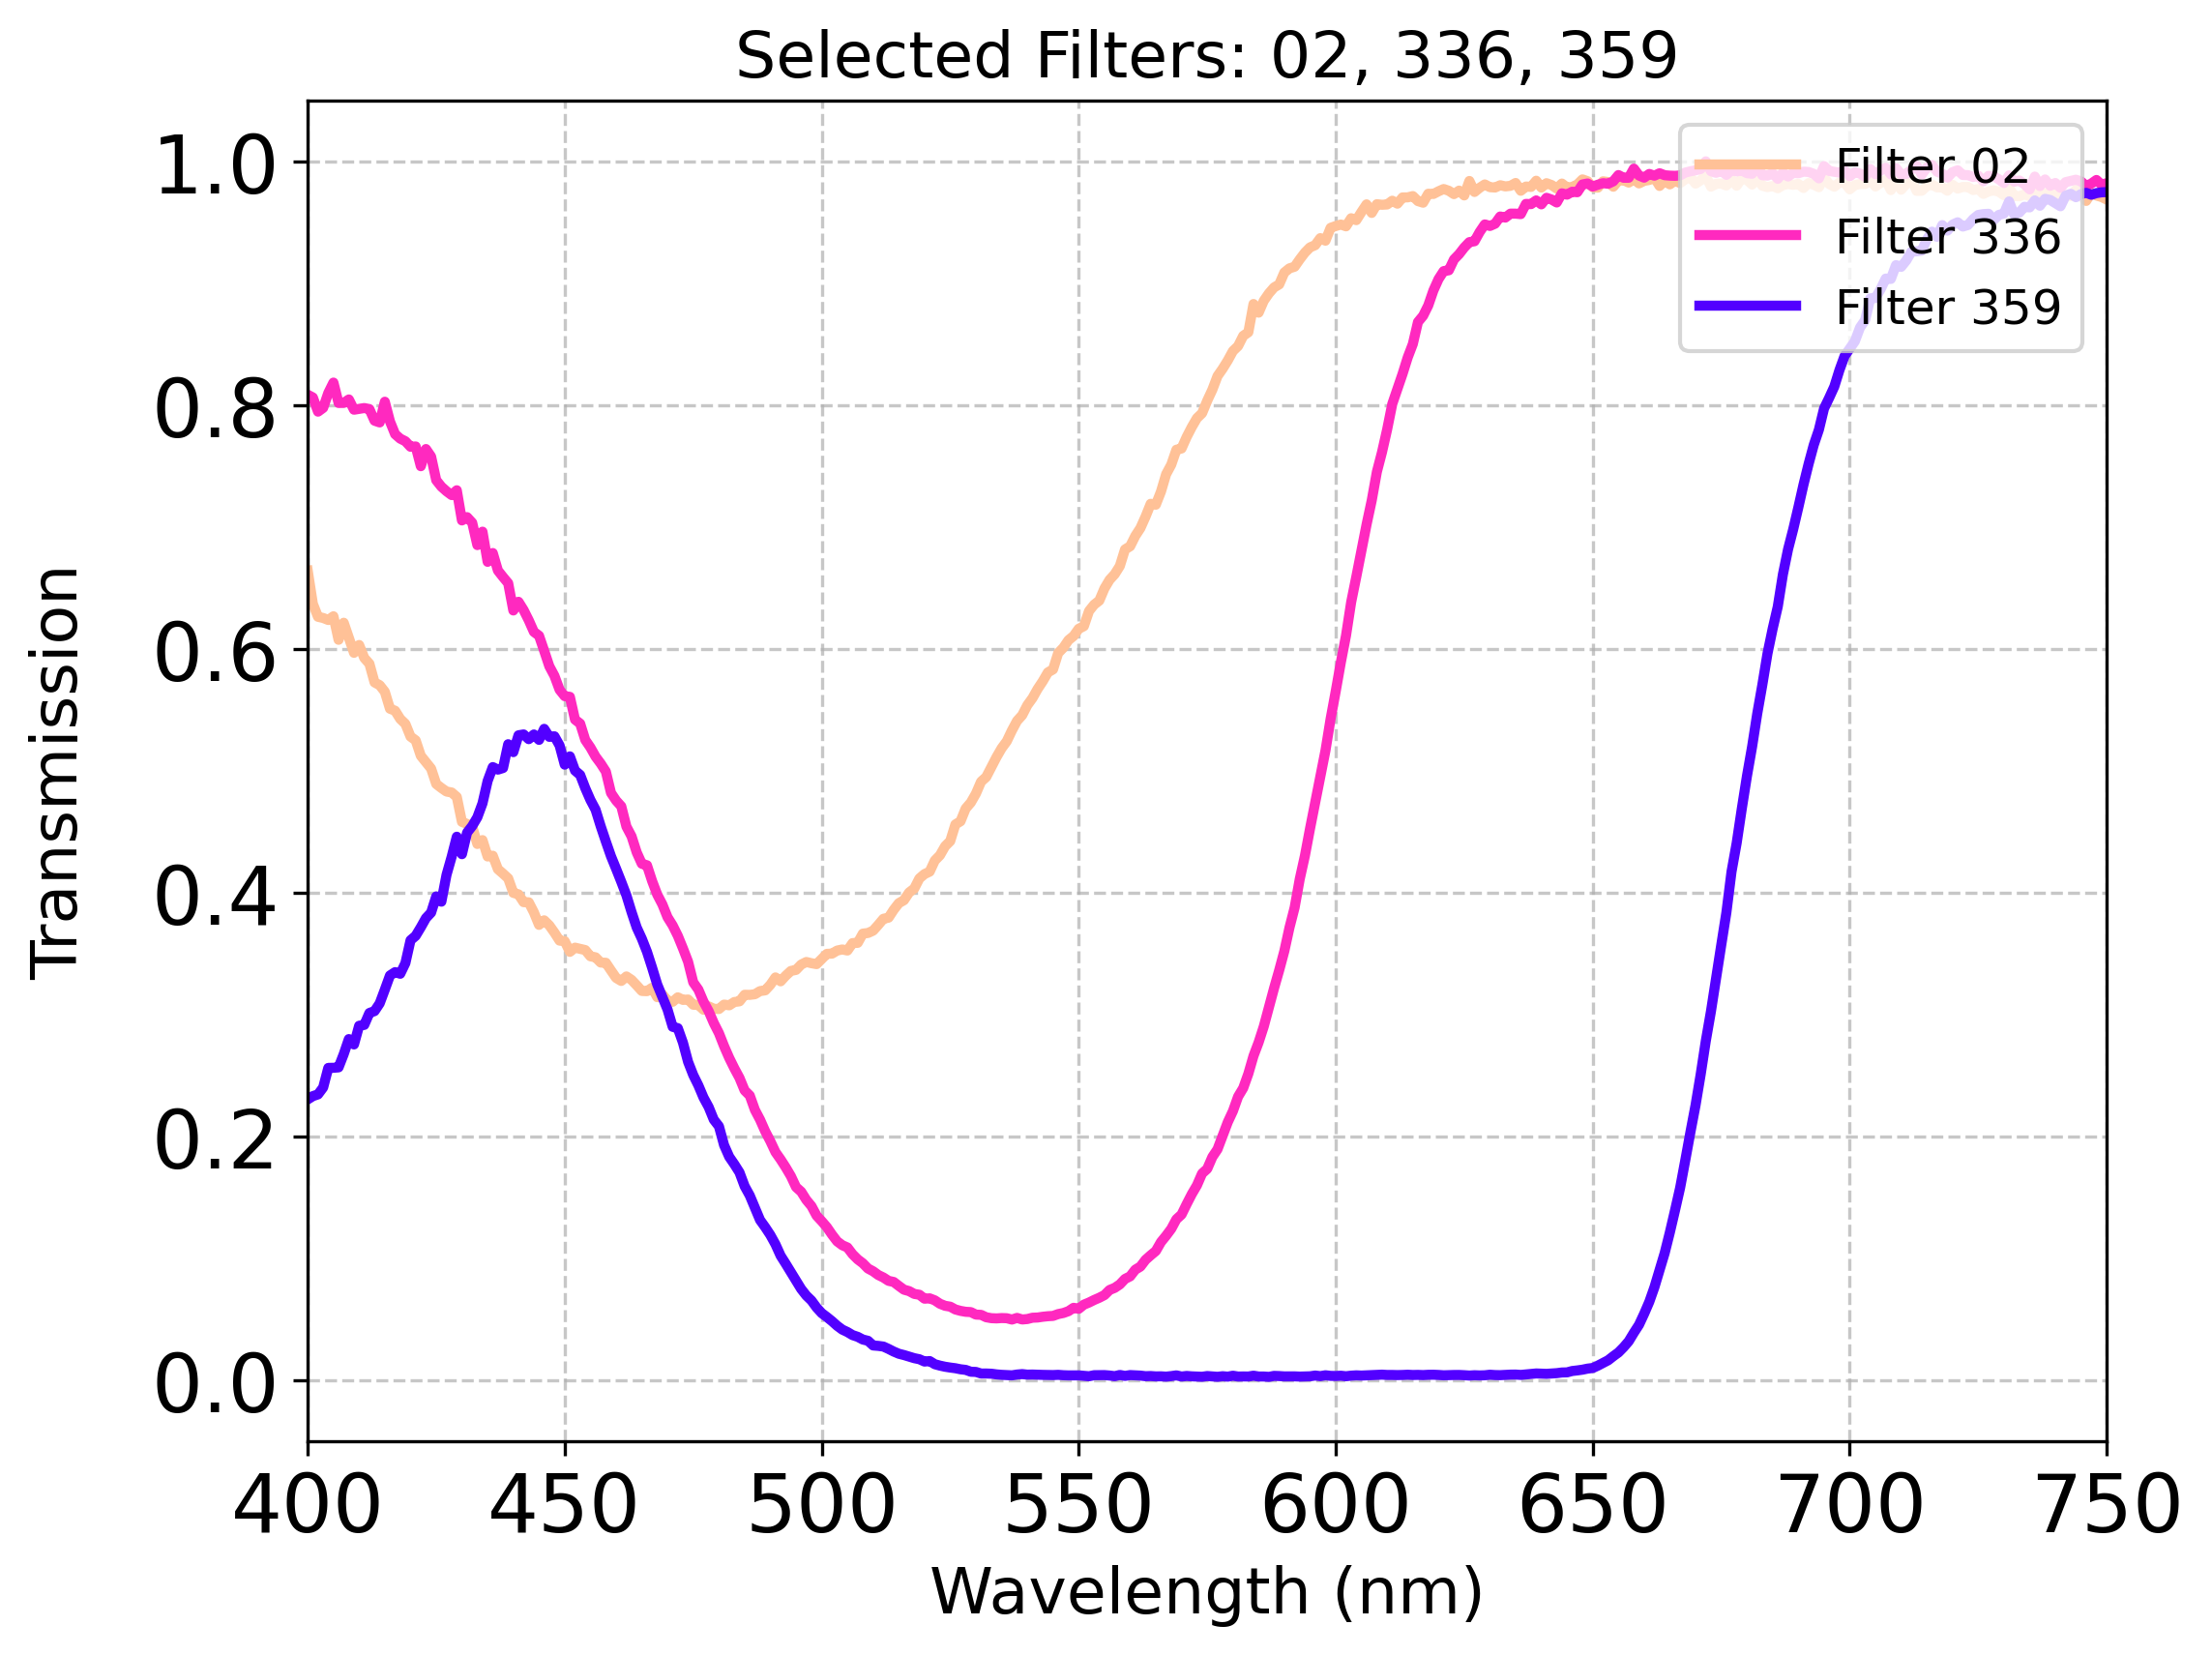
\includegraphics[width=\linewidth]{media/measured_k3_trans.png}
    \caption{Transmission functions of selected filters}
\end{subfigure}
\caption{$k=3$ Transmission functions and location on gamut}
\label{fig:k3Transmissions}
\end{figure}

\subsubsection{Solution for $k=4$}

We see a noticeable improvement in MSE and in $\dE$ with $k=4$, measuring 1.09, slightly above the 'just noticeable difference' of 1.0 \cite{lindstrom2008delta}. 
The CAVE dataset reconstruction approaches the ground truth reconstruction, although the human eye may observe slight differences in the overall image. 

\begin{figure}[H]
\centering
\begin{subfigure}{.49\linewidth}
    \centering
    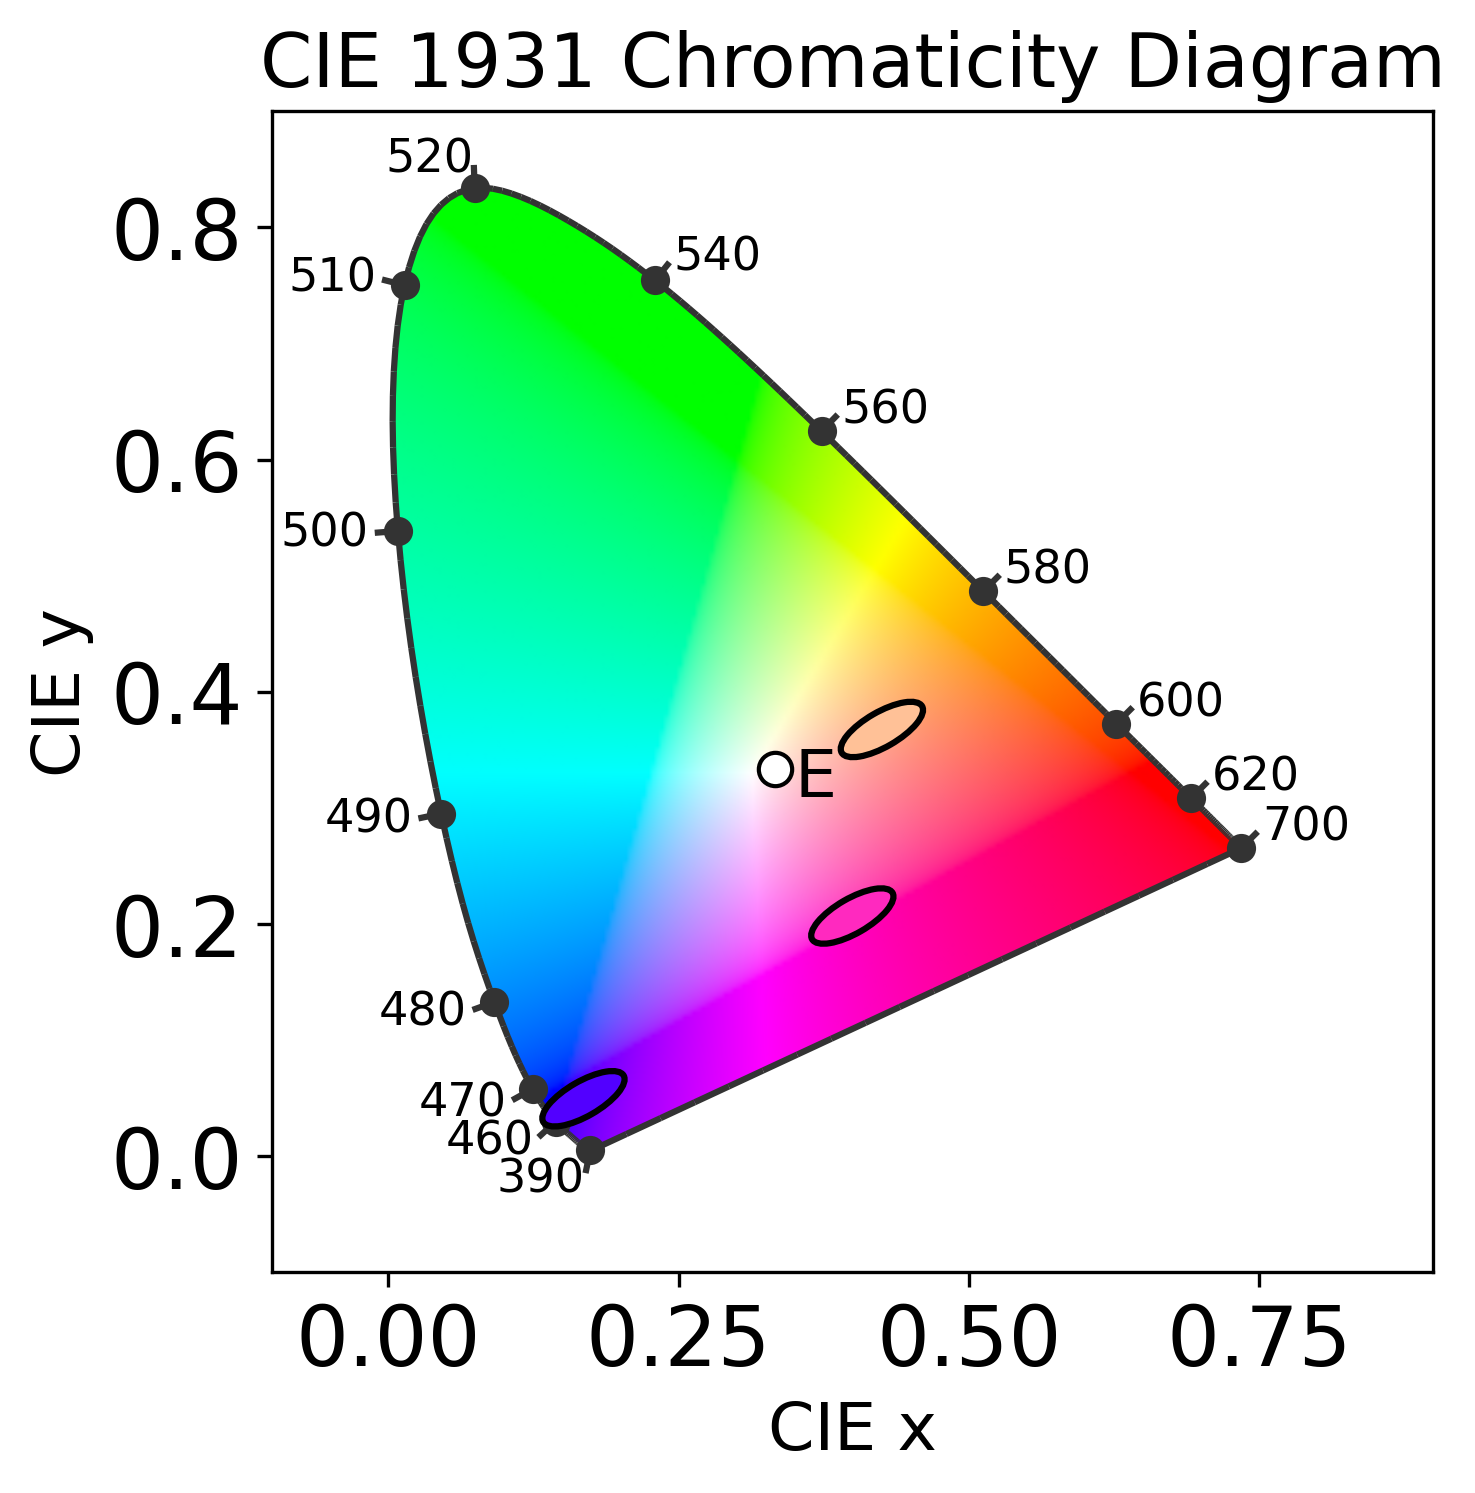
\includegraphics[width=\linewidth]{media/measured_k3_gamut.png}
    \caption{Best XYZ reconstruction}
\end{subfigure}%
\begin{subfigure}{.49\linewidth}
    \centering
    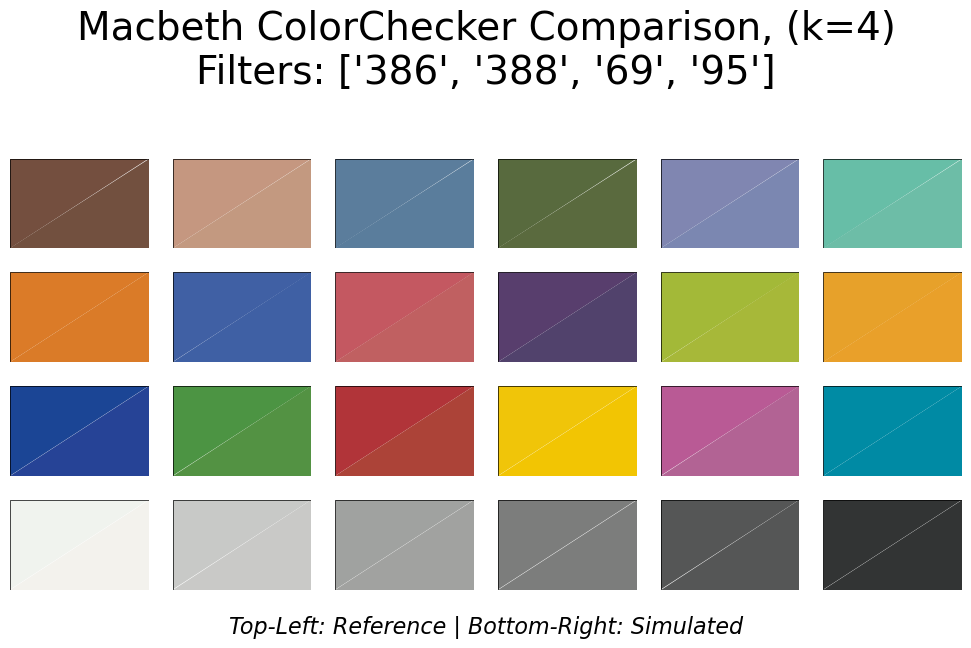
\includegraphics[width=\linewidth]{media/measured_k4_macbeth.png}
    \caption{Macbeth Color Checker comparison}
\end{subfigure}
\begin{subfigure}{.49\linewidth}
    \centering
    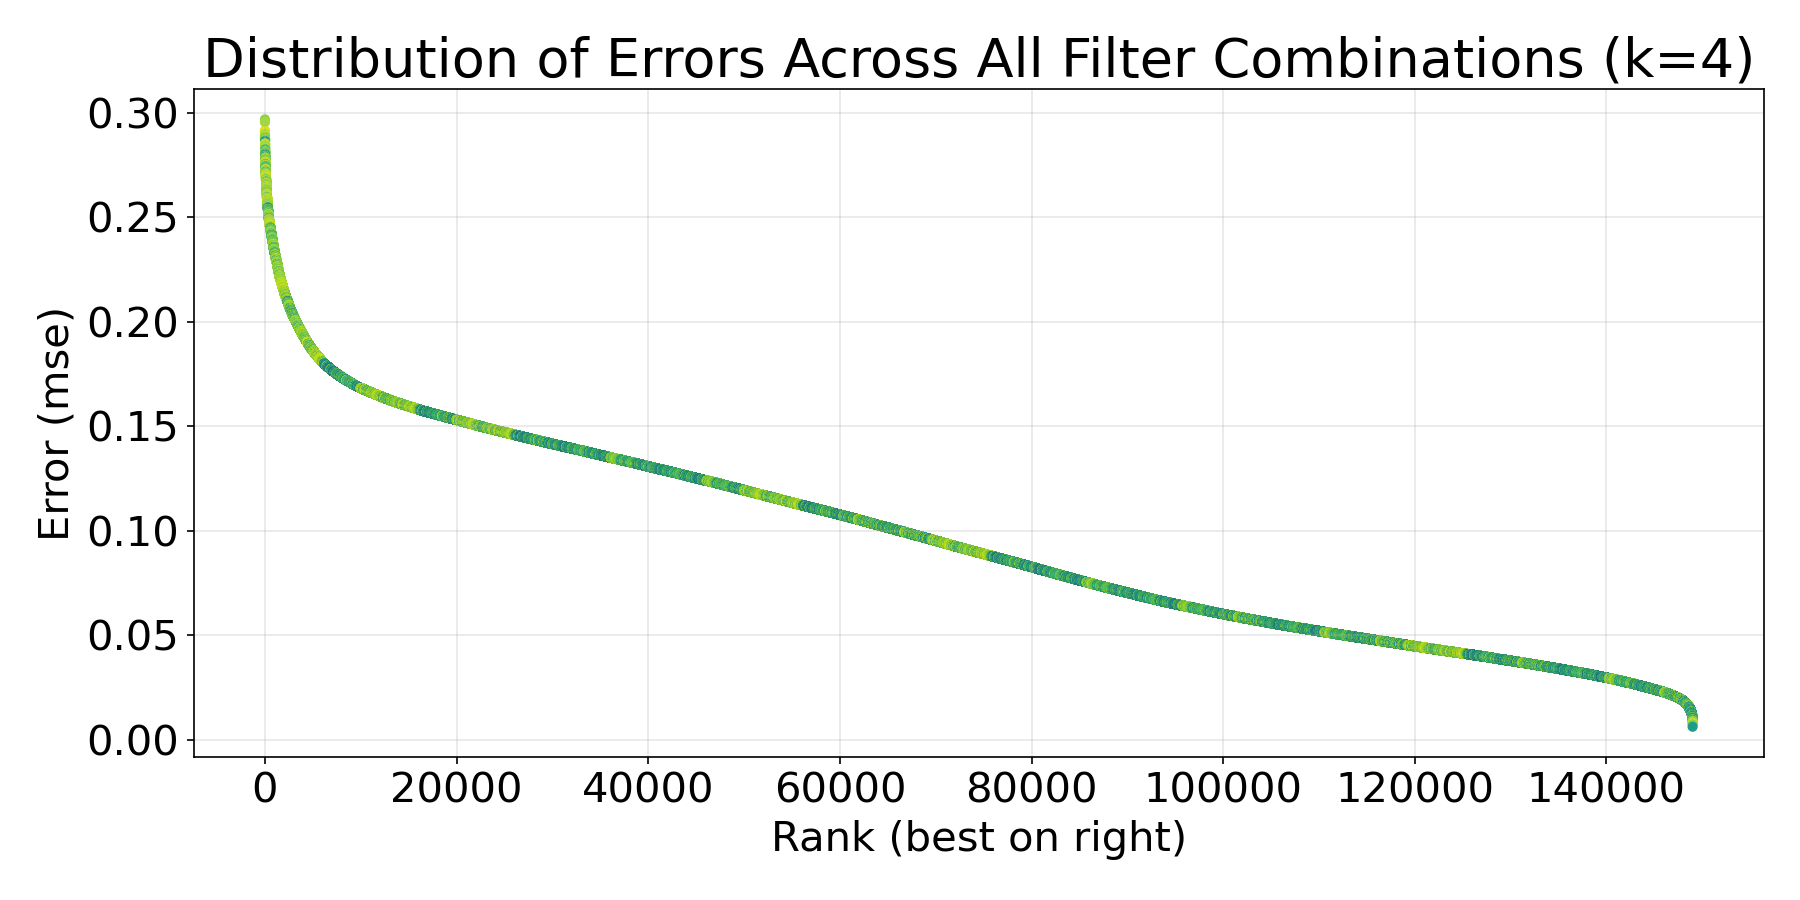
\includegraphics[width=\linewidth]{media/measured_k4_errors.png}
    \caption{Error distribution across combinations}
\end{subfigure}%
\begin{subfigure}{.49\linewidth}
    \centering
    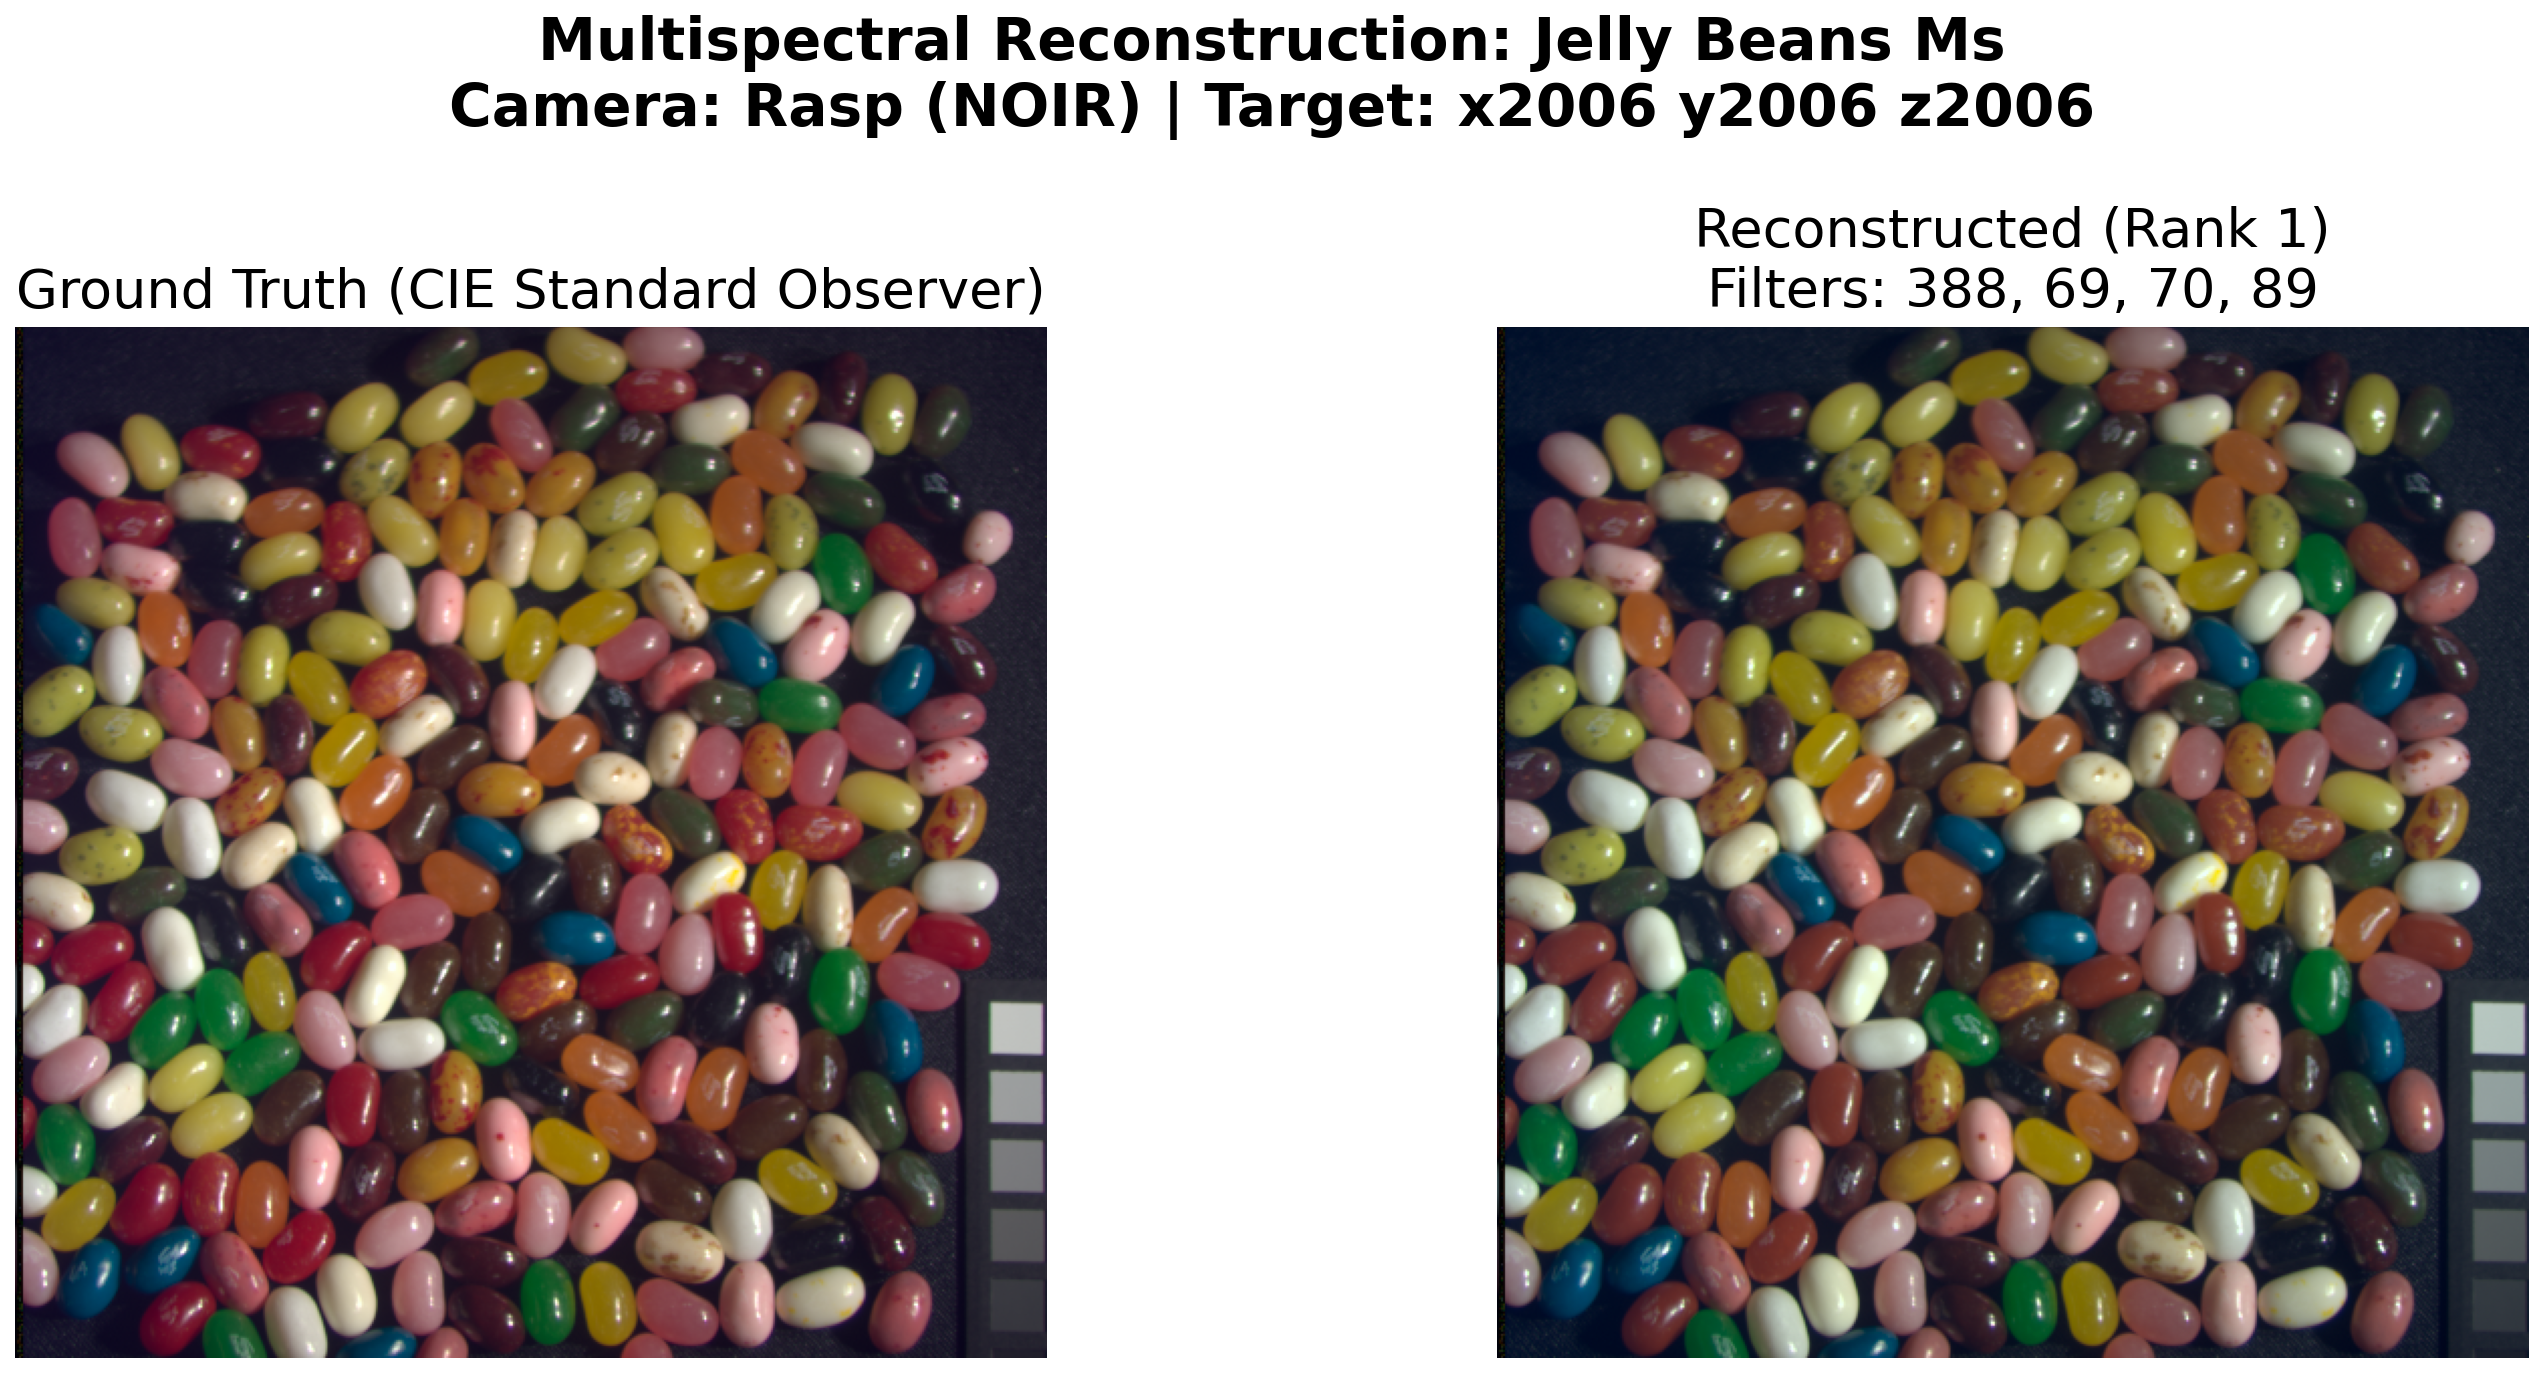
\includegraphics[width=\linewidth]{media/measured_k4_cave.png}
    \caption{CAVE render of combination}
\end{subfigure}
\caption{Supergel results for $k=4$.}
\label{fig:k4spectral}
\end{figure}

In comparison to the $k=3$ case, we see relatively little transmission above the 650nm range, yet a reconstruction may struggle to recreate red hues and the 15th Macbeth patch, the dark red patch, has a $\dE$ of about 9, significantly worse than the rest. 
Conceptually, we can see that the gamut has little coverage over the red corner of the 1931 color gamut.

\begin{figure}[H]
\centering
\begin{subfigure}{.40\linewidth}
    \centering
    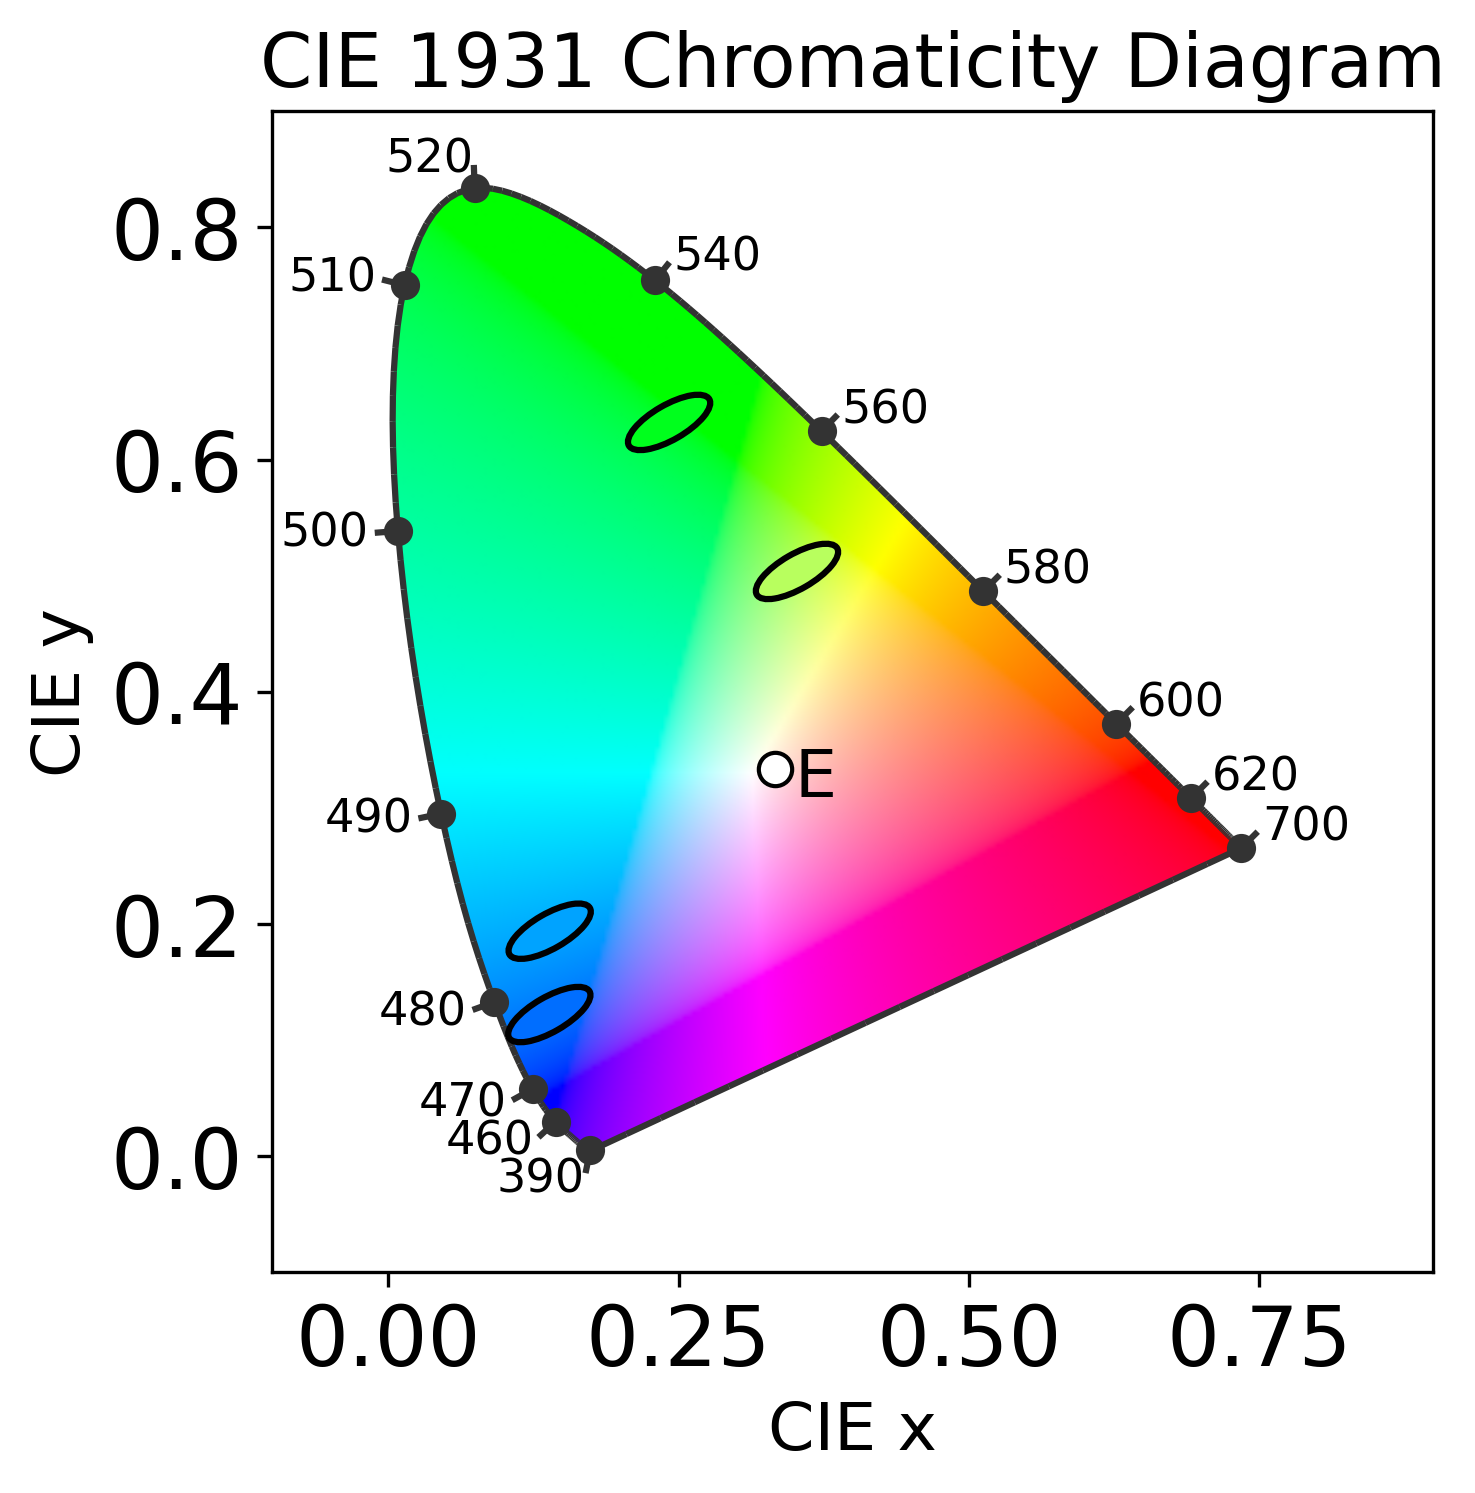
\includegraphics[width=\linewidth]{media/measured_k4_gamut.png}
    \caption{Location on CIE 1931 Color Gamut}
\end{subfigure}%
\begin{subfigure}{.55\linewidth}
    \centering
    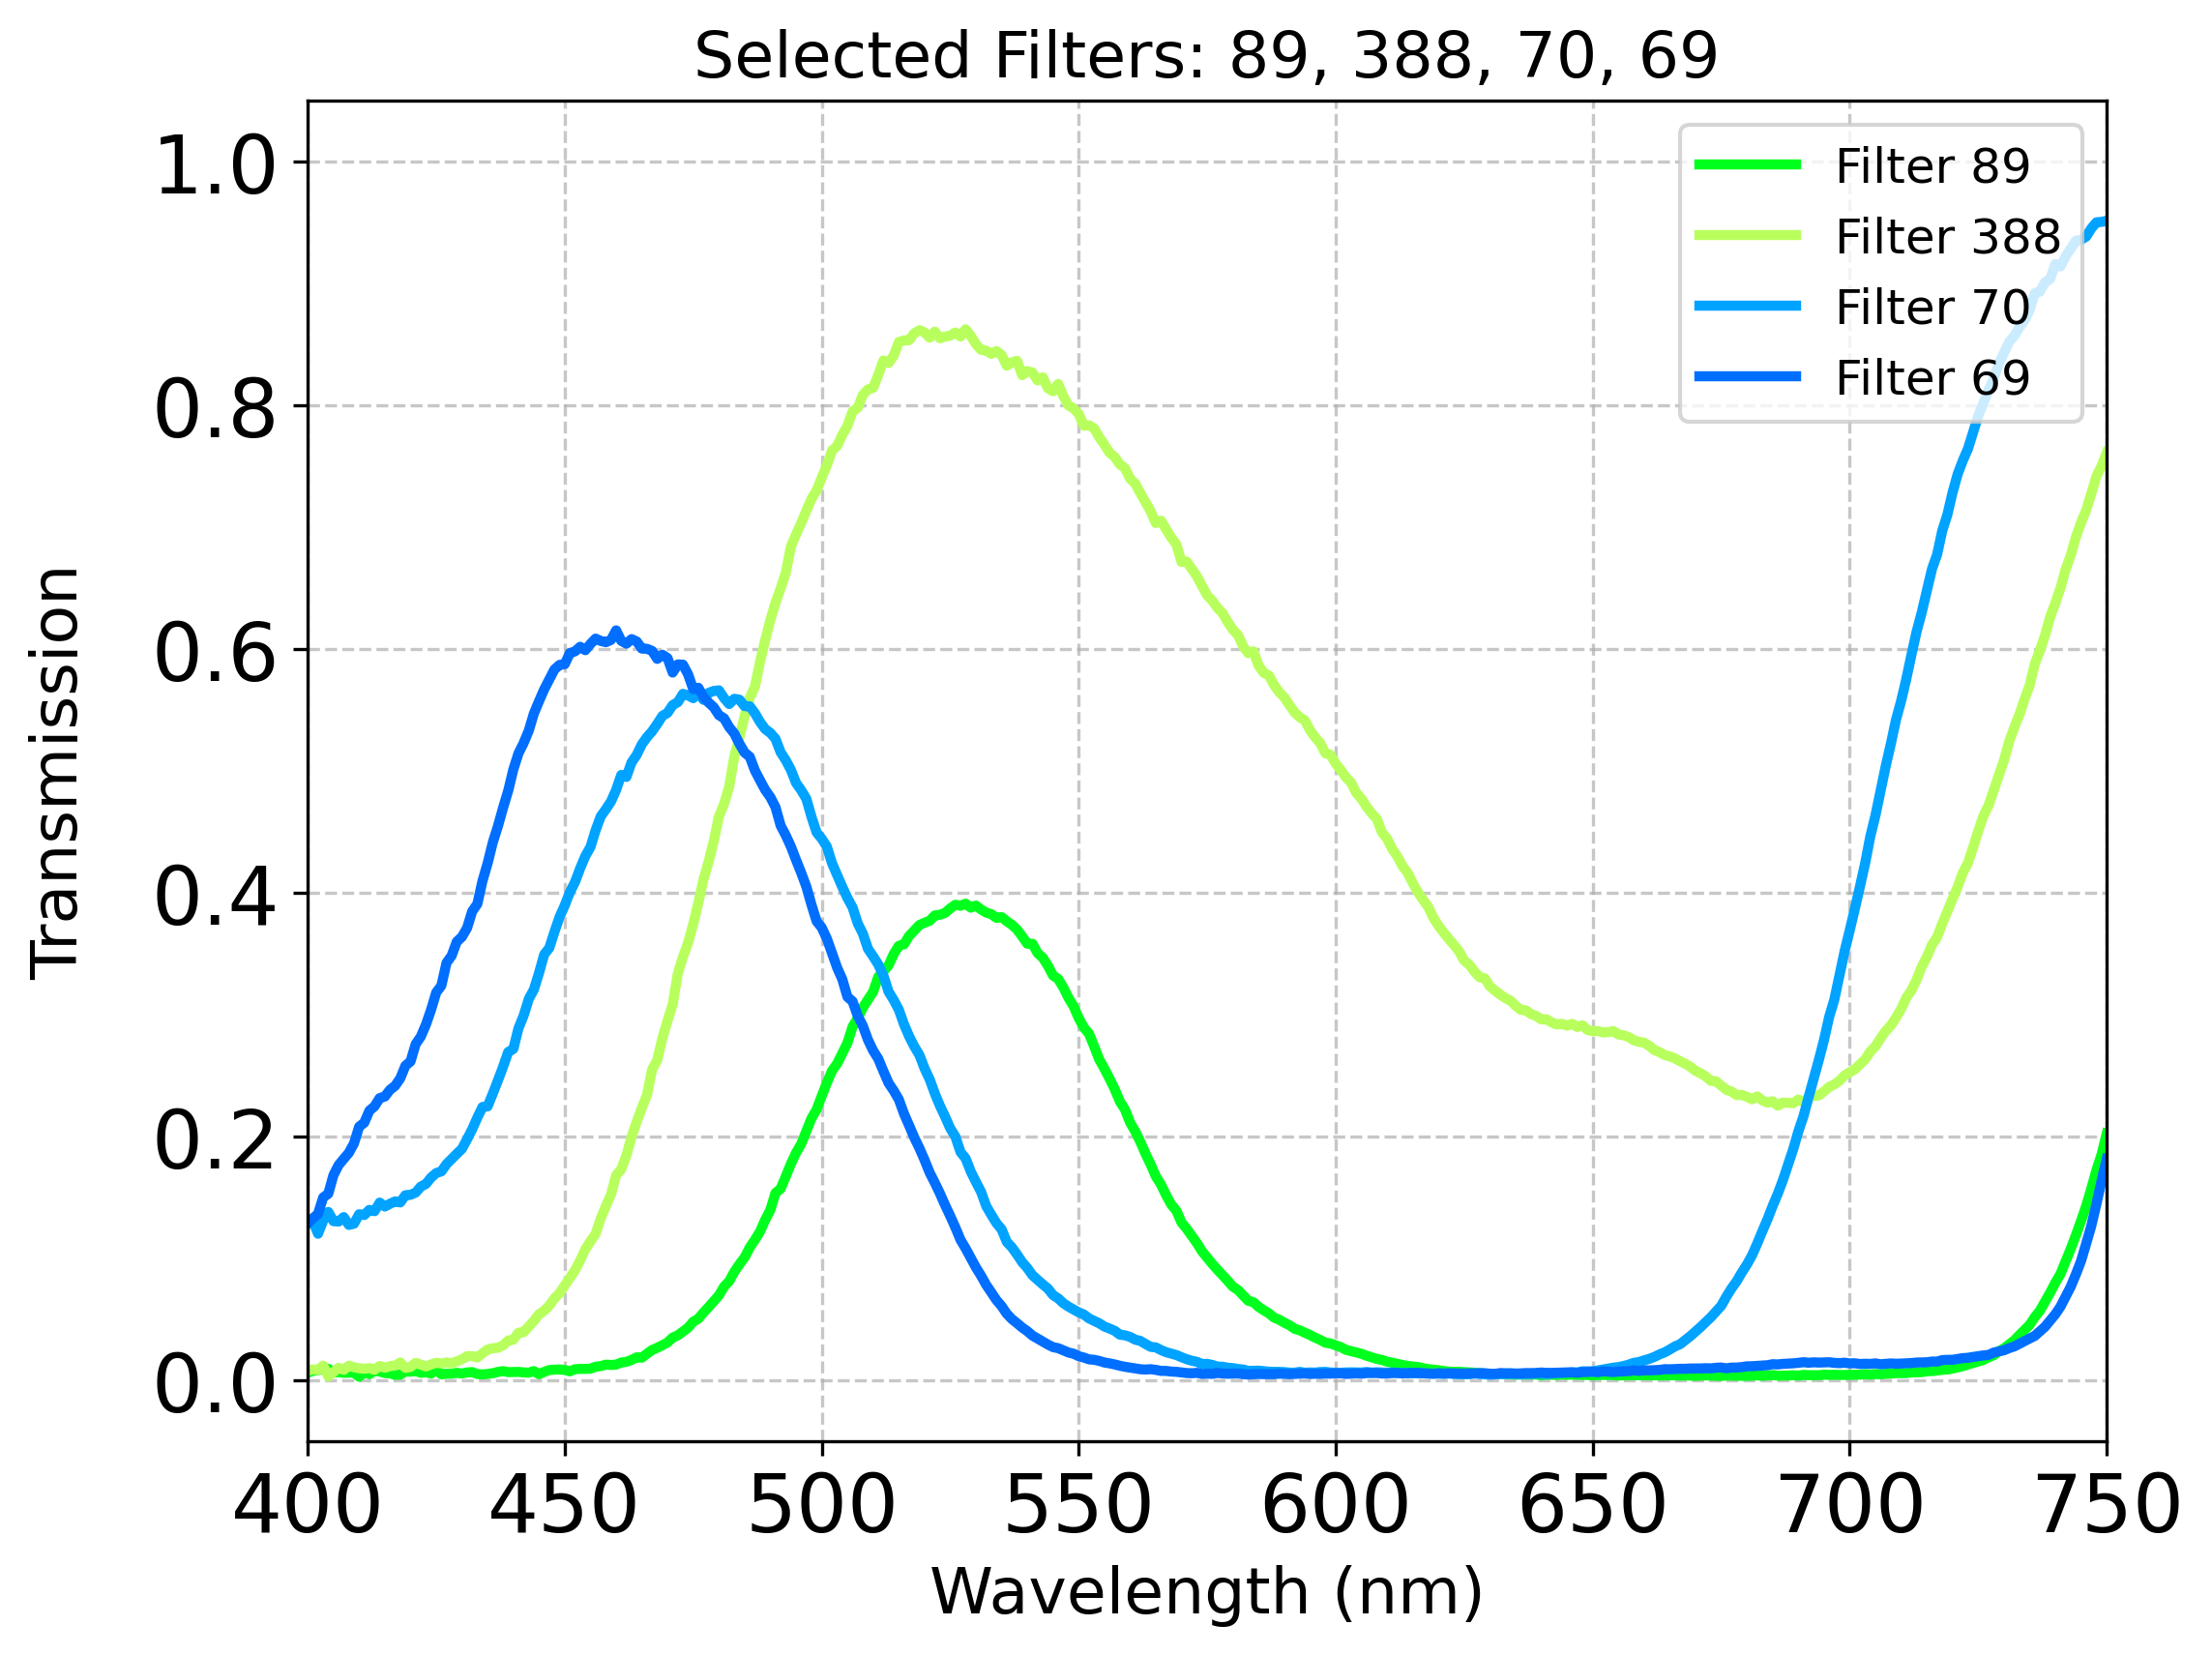
\includegraphics[width=\linewidth]{media/measured_k4_transmission.png}
    \caption{Transmission functions of selected filters}
\end{subfigure}
\caption{$k=4$ Transmission functions and location on gamut}
\label{fig:k4Transmissions}
\end{figure}

\subsubsection{Solution for $k=5$}


For the $k=5$ case, the $\dE$ reaches .35 and clearly improves on the reconstruction of the target curves. 
Importantly, the worst individual $\dE$ recorded amongst the Macbeth patches are patches 2 and 15, the tan and red patches. 
The cave reconstruction is quite hard to distinguish from the ground truth. 

\begin{figure}[H]
\centering
\begin{subfigure}{.49\linewidth}
    \centering
    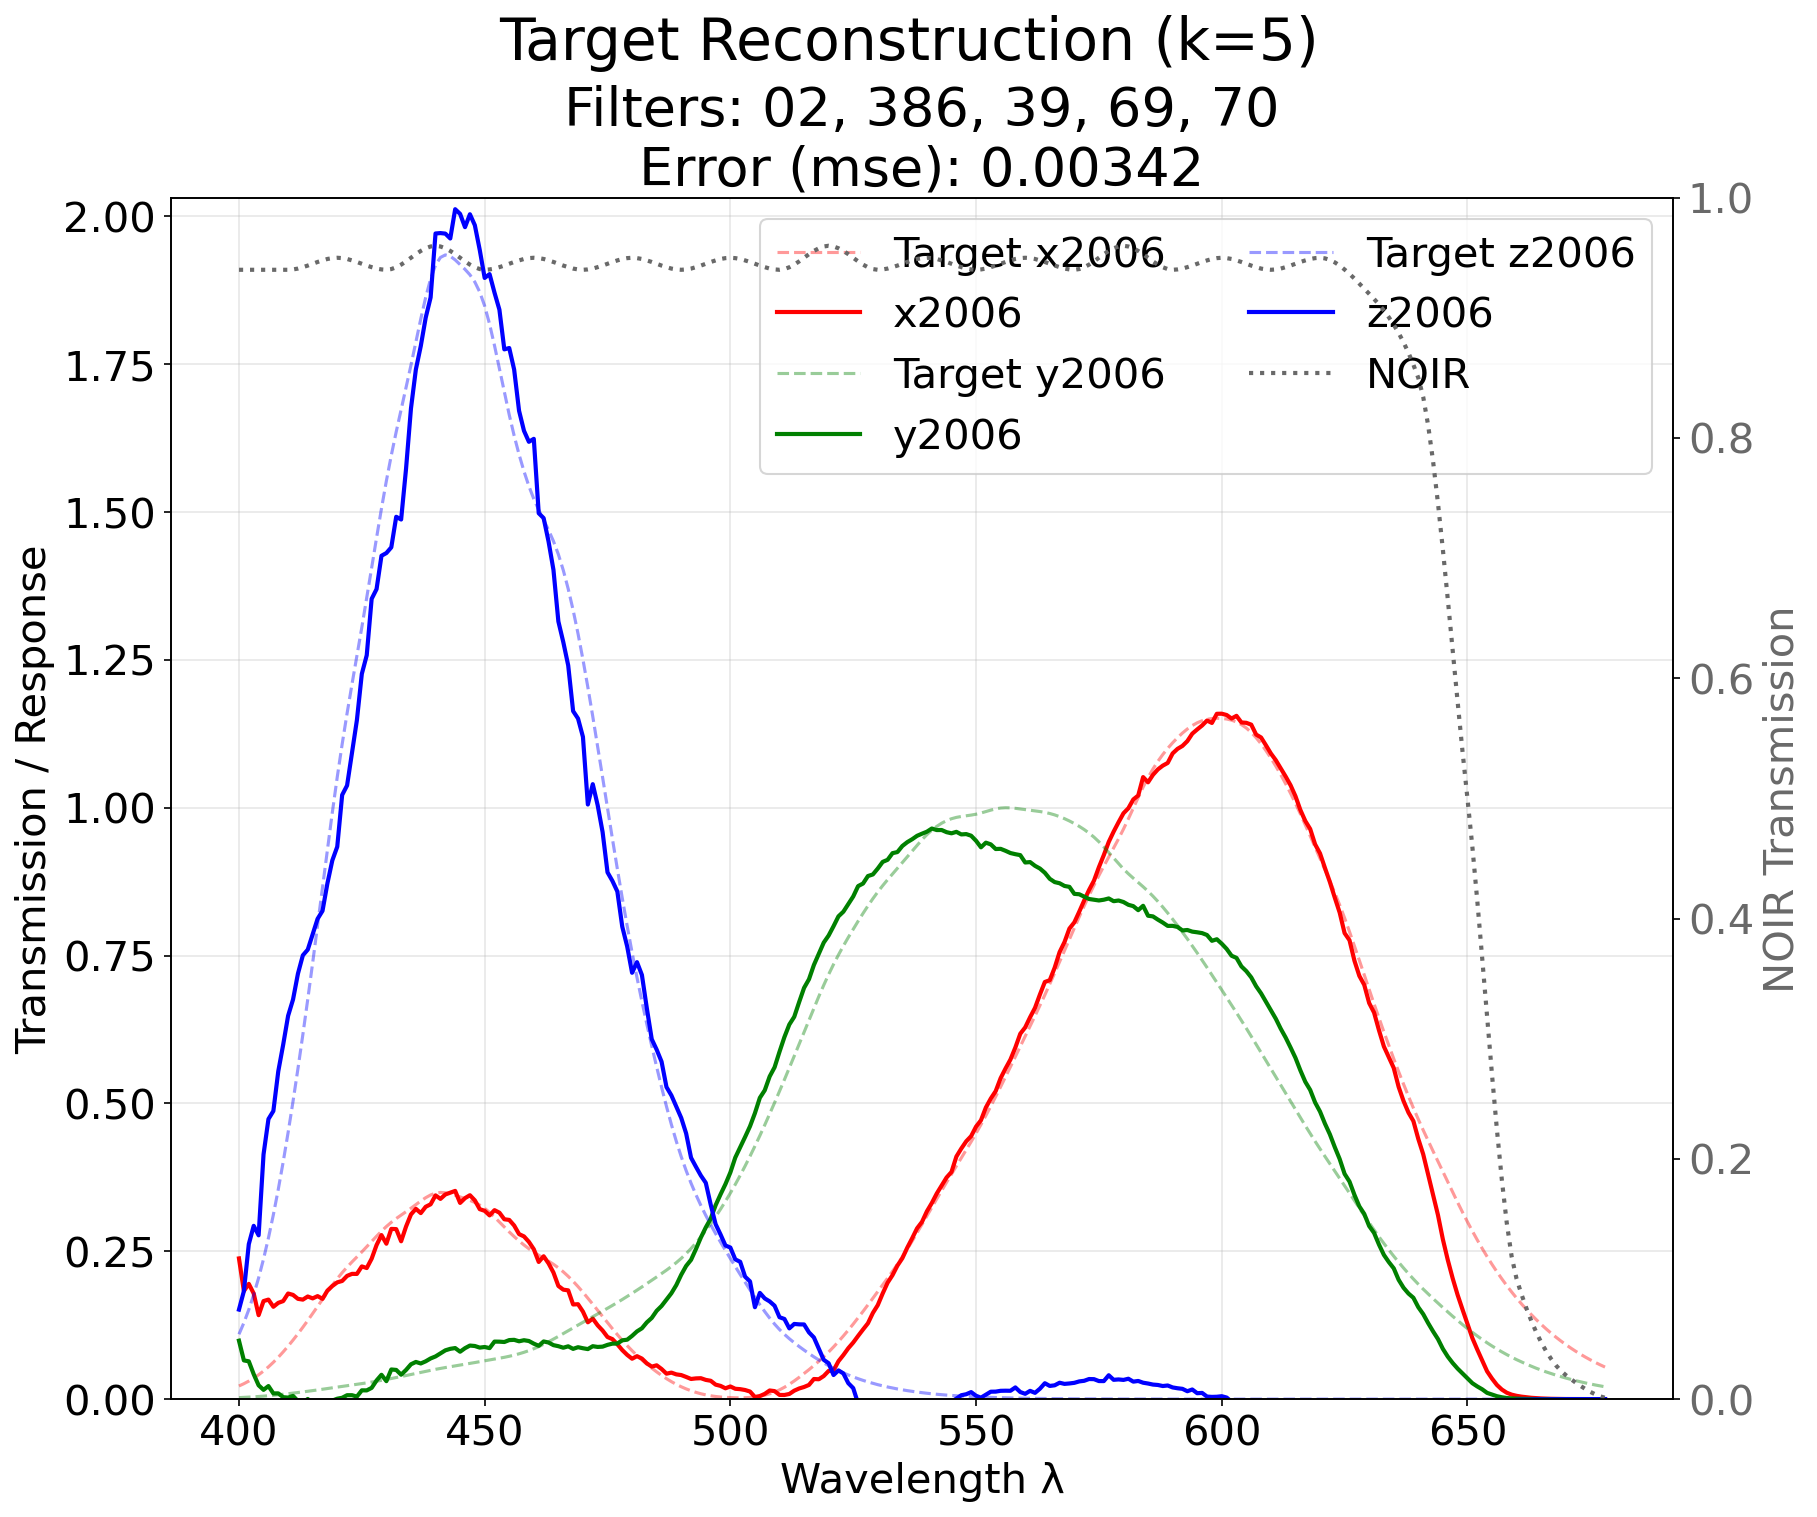
\includegraphics[width=\linewidth]{media/measured_k5_spectra.png}
    \caption{Best XYZ reconstruction}
\end{subfigure}%
\begin{subfigure}{.49\linewidth}
    \centering
    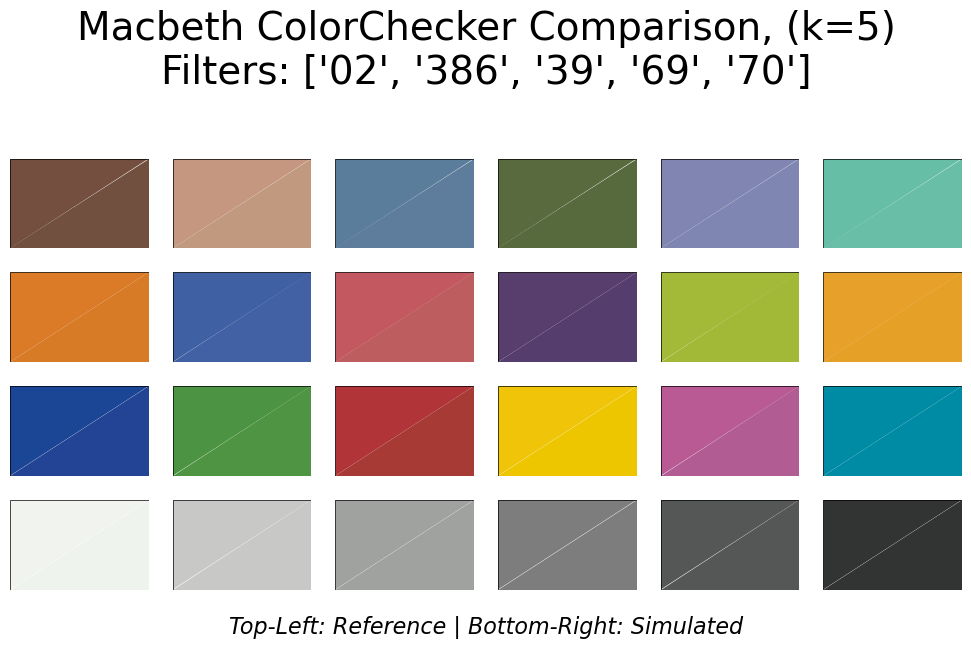
\includegraphics[width=\linewidth]{media/measured_k5_macbeth.png}
    \caption{Macbeth Color Checker comparison}
\end{subfigure}
\begin{subfigure}{.49\linewidth}
    \centering
    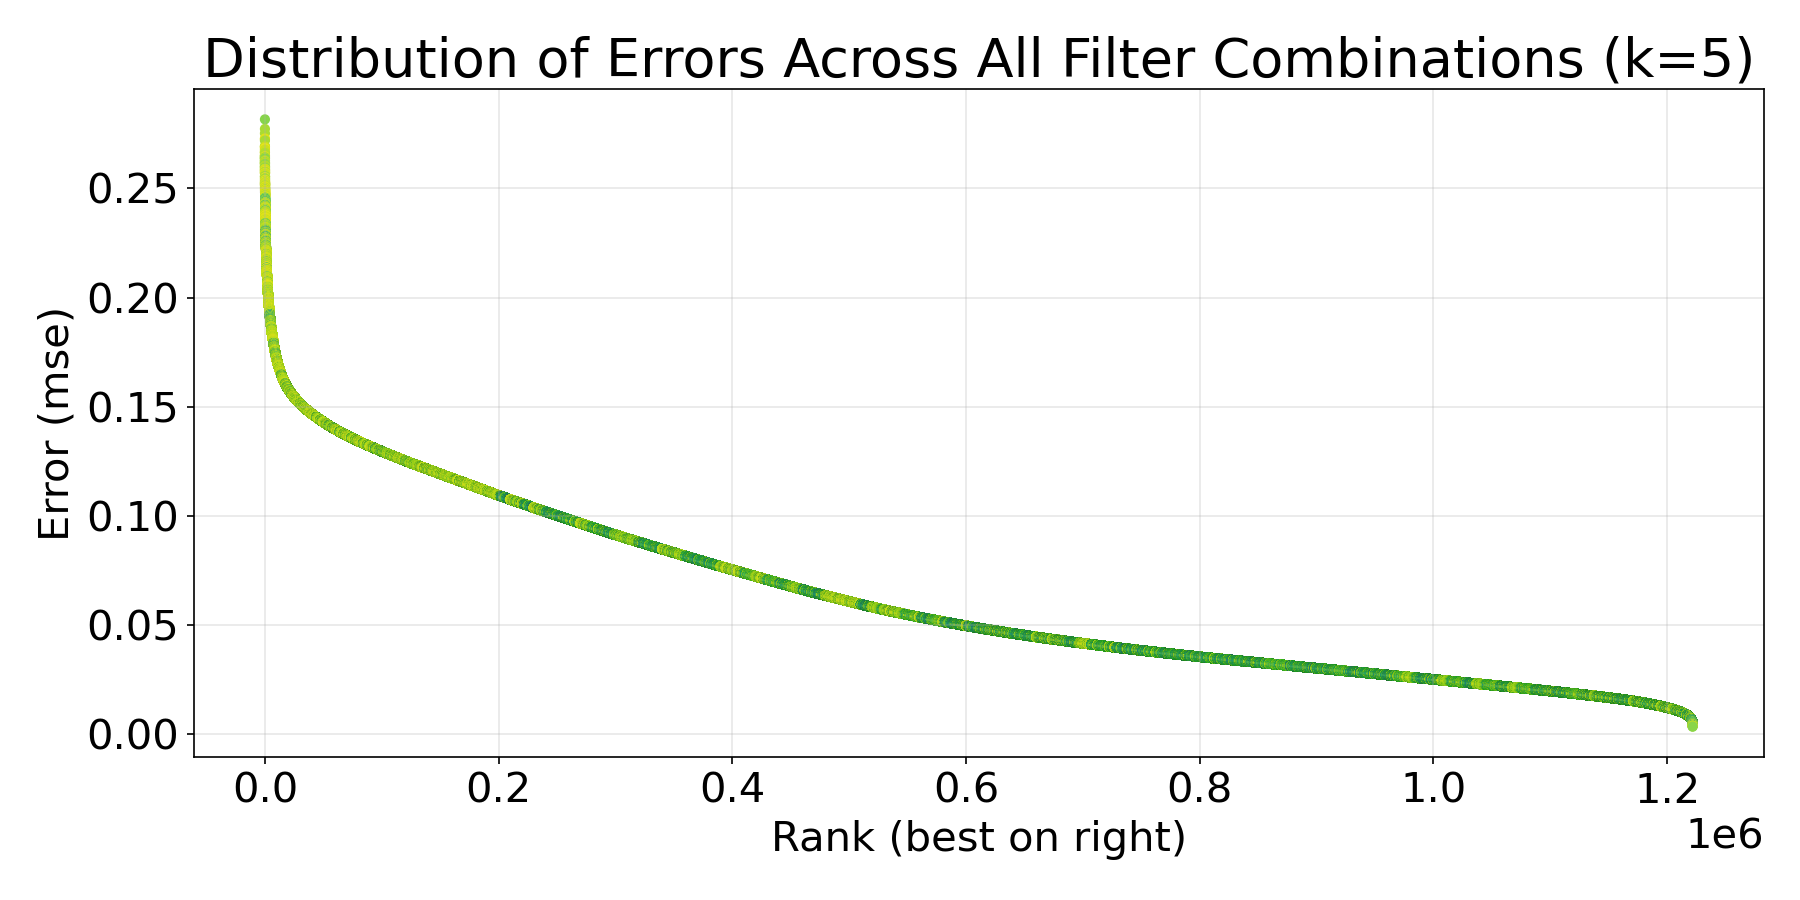
\includegraphics[width=\linewidth]{media/measured_k5_errors.png}
    \caption{Error distribution across combinations}
\end{subfigure}%
\begin{subfigure}{.49\linewidth}
    \centering
    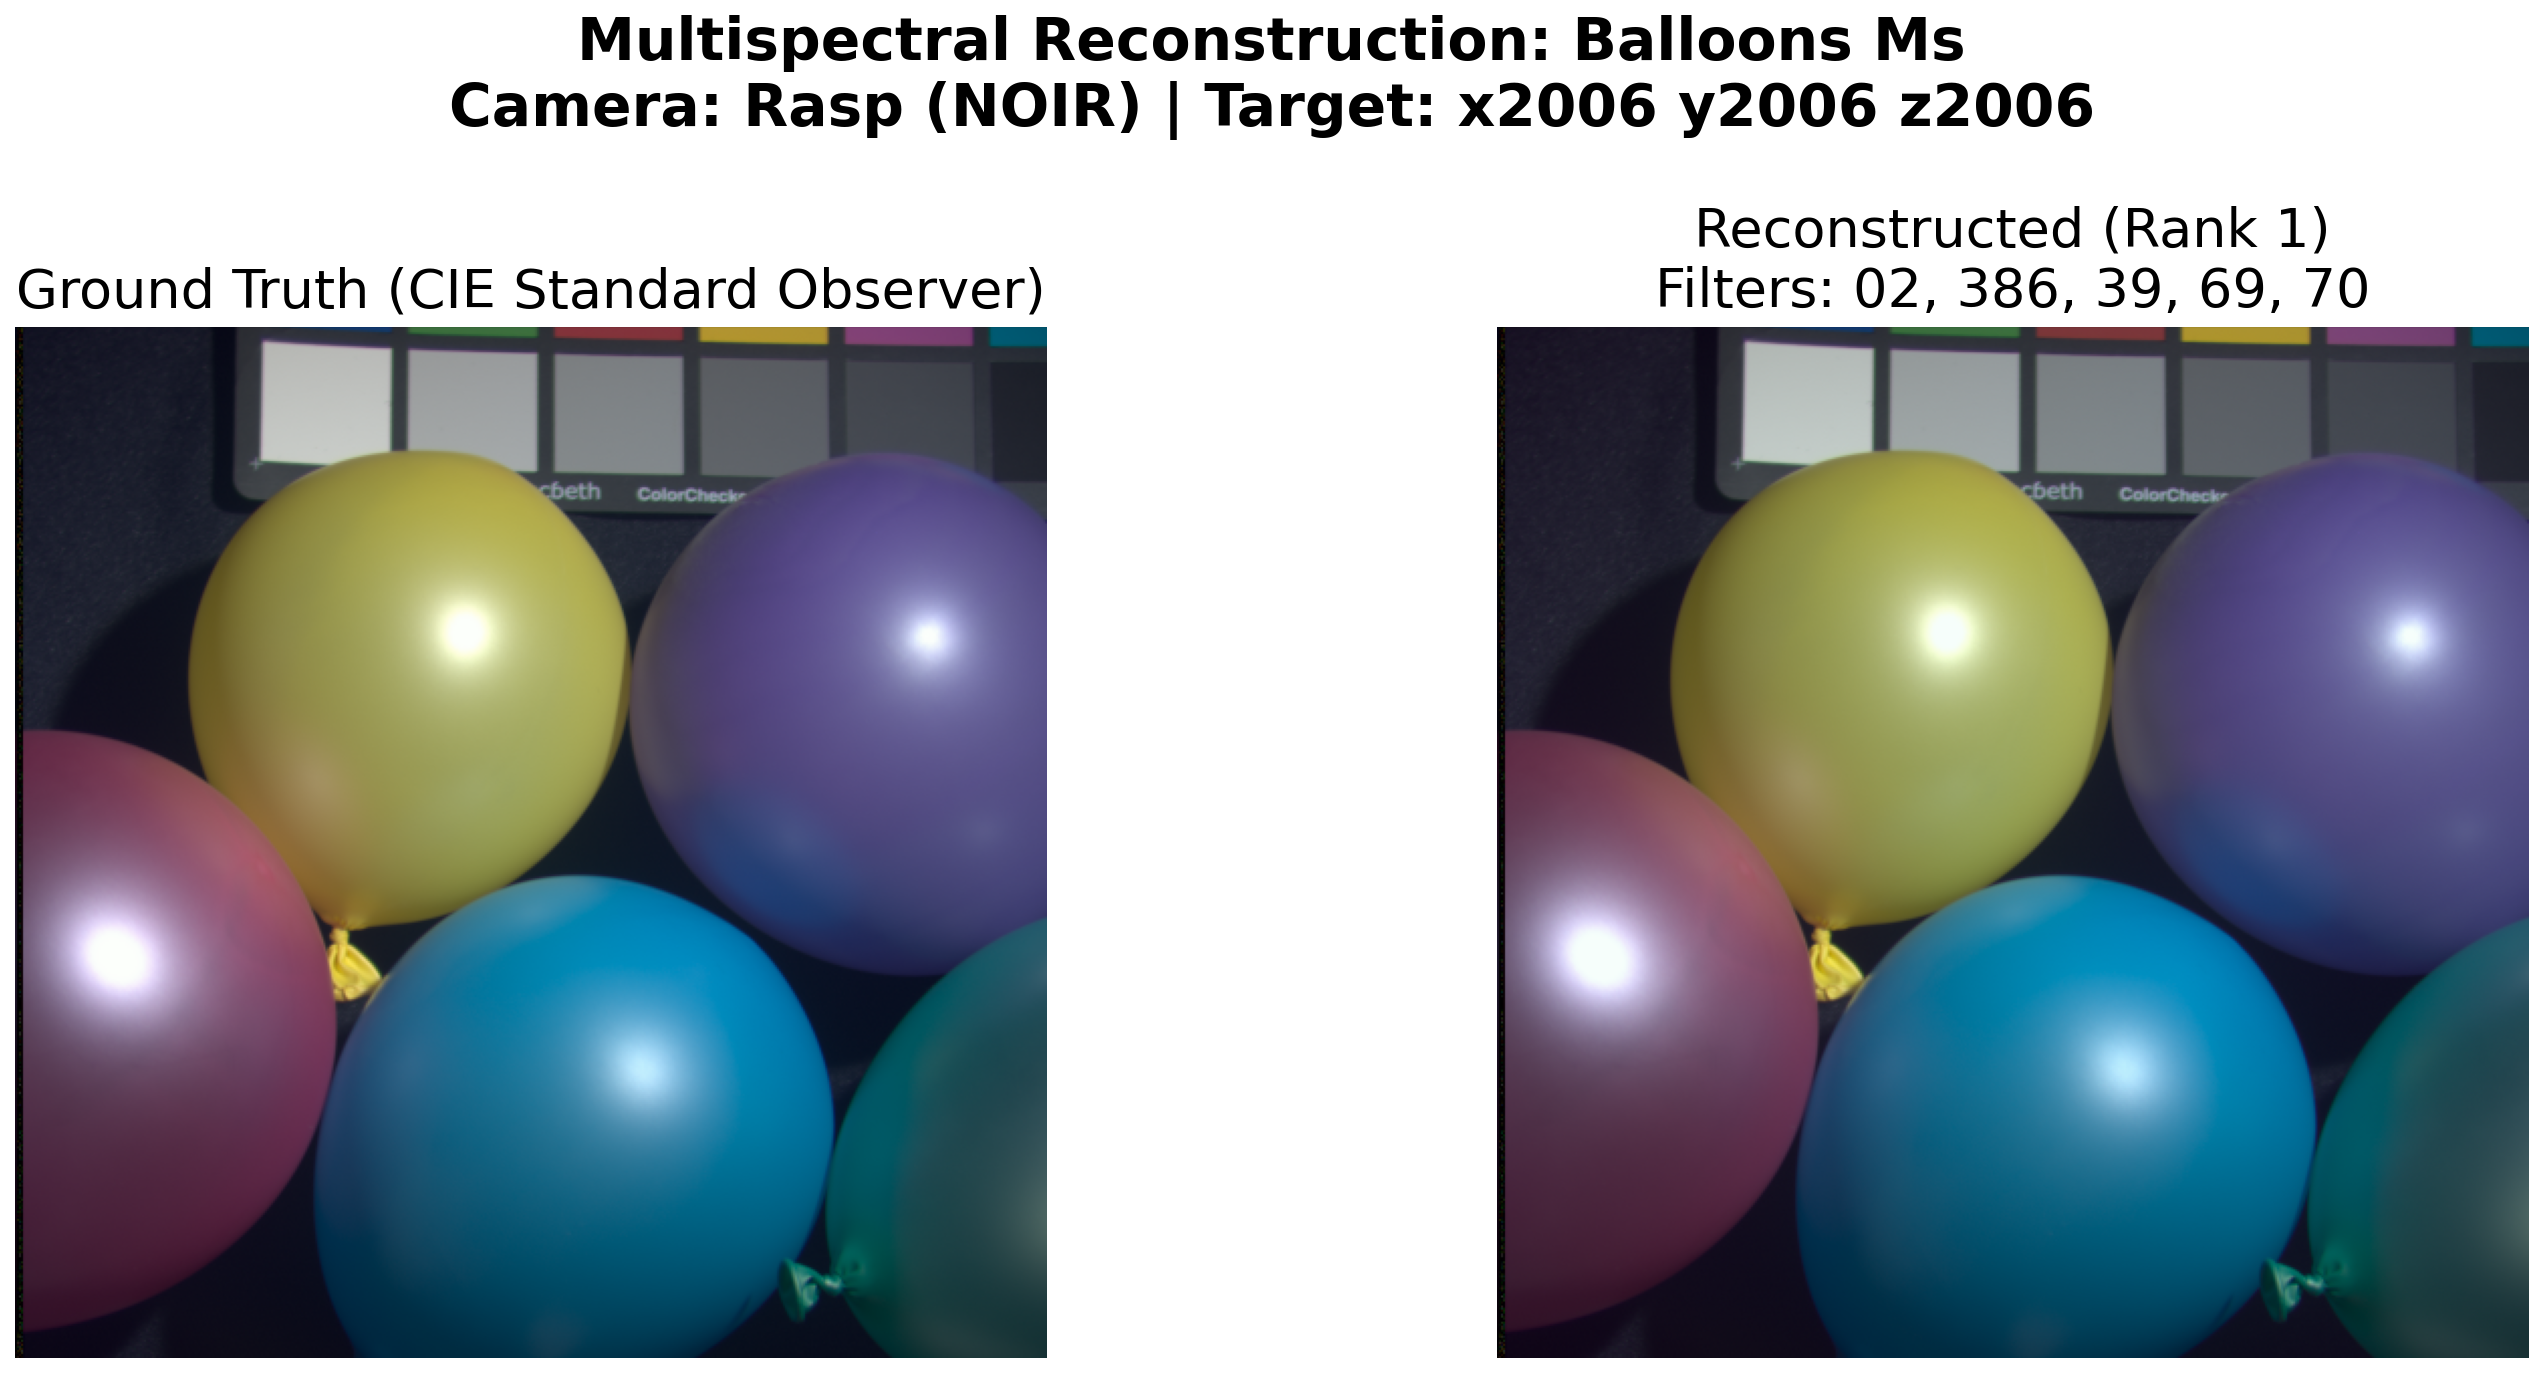
\includegraphics[width=\linewidth]{media/measured_k5_cave.png}
    \caption{CAVE dataset rendering}
\end{subfigure}
\caption{Supergel results for $k=5$.}
\label{fig:k5spectral}
\end{figure}


\begin{figure}[H]
\centering
\begin{subfigure}{.40\linewidth}
    \centering
    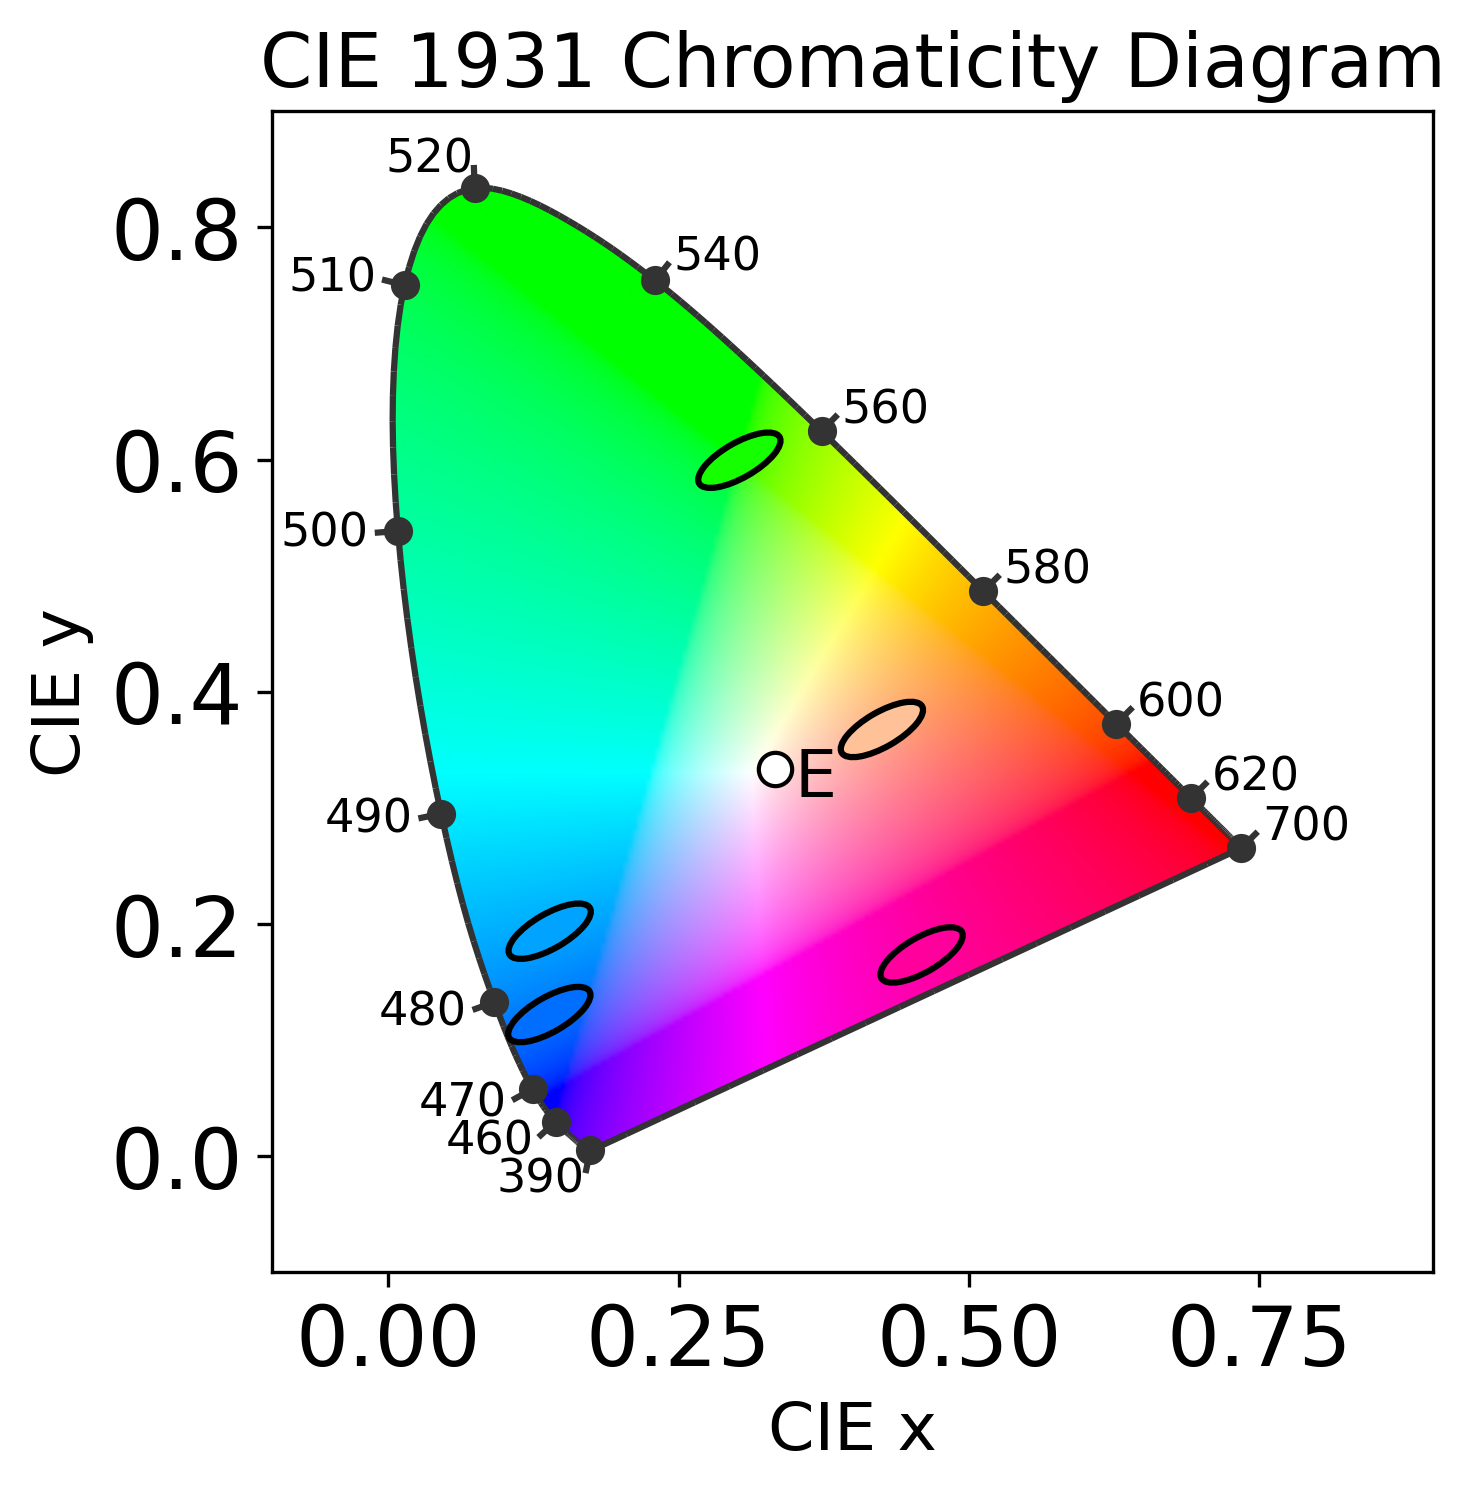
\includegraphics[width=\linewidth]{media/measured_k5_gamut.png}
    \caption{Location on CIE 1931 Color Gamut}
\end{subfigure}%
\begin{subfigure}{.55\linewidth}
    \centering
    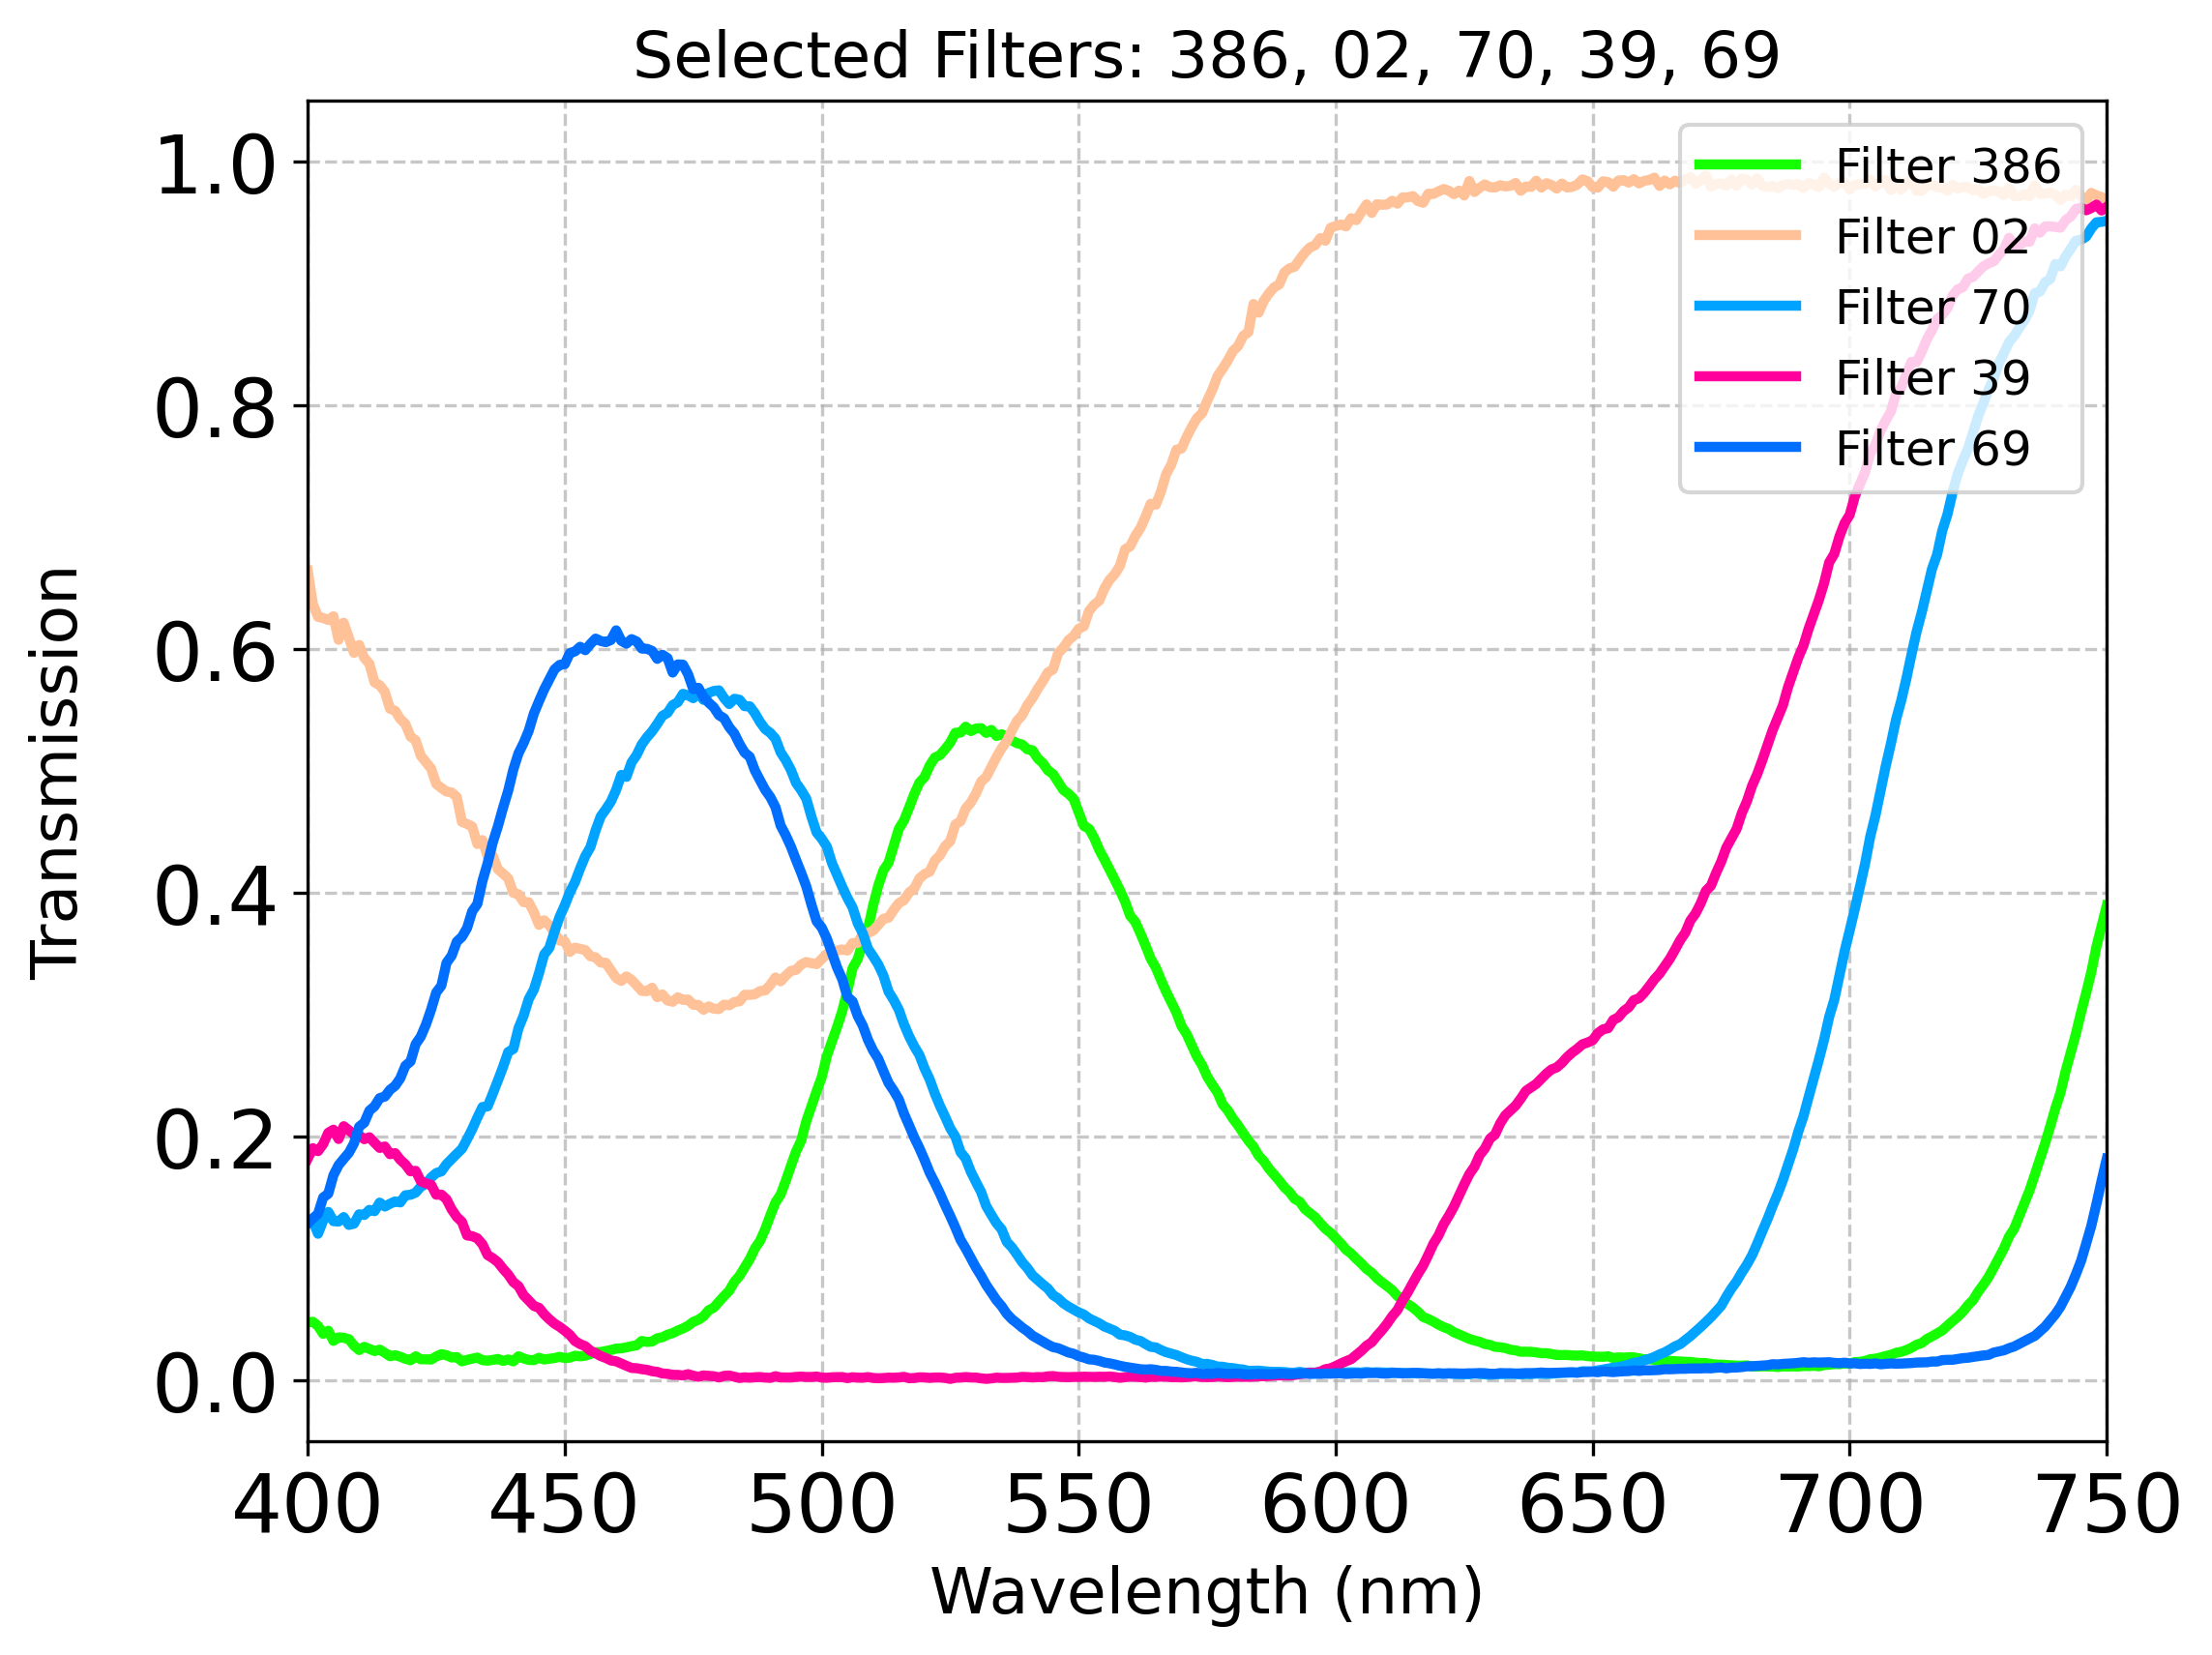
\includegraphics[width=\linewidth]{media/measured_k5_transmission.png}
    \caption{Transmission functions of selected filters}
\end{subfigure}
\caption{$k=5$ Transmission functions and location on gamut}
\label{fig:k5Transmissions}
\end{figure}

Additional captures from the CAVE dataset are included in the appendix. 

\subsection{CIE 2006 10-degree CMF}

We focus our prior research on the 2-degree CMF derived by Stockman \& Sharpe \cite{STOCKMAN20001711}, but also show that with minimal overhead, we can provide an effective filter selection for the 10 degree color matching functions enumerated in the same body of research. 
In this context, the 'degree' refers to the field of view of the observer.
While we only achieve $\dE<1$ at $k=6$, this is a reasonable result. 
We note that the original PCA algorithm performs worse than the PCA2 algorithm (Algorithm 3), the former failing to find a selection which identifies a combination with $\dE<1$.

\begin{figure}[H]
\centering
\begin{subfigure}{.64\linewidth}
    \centering
    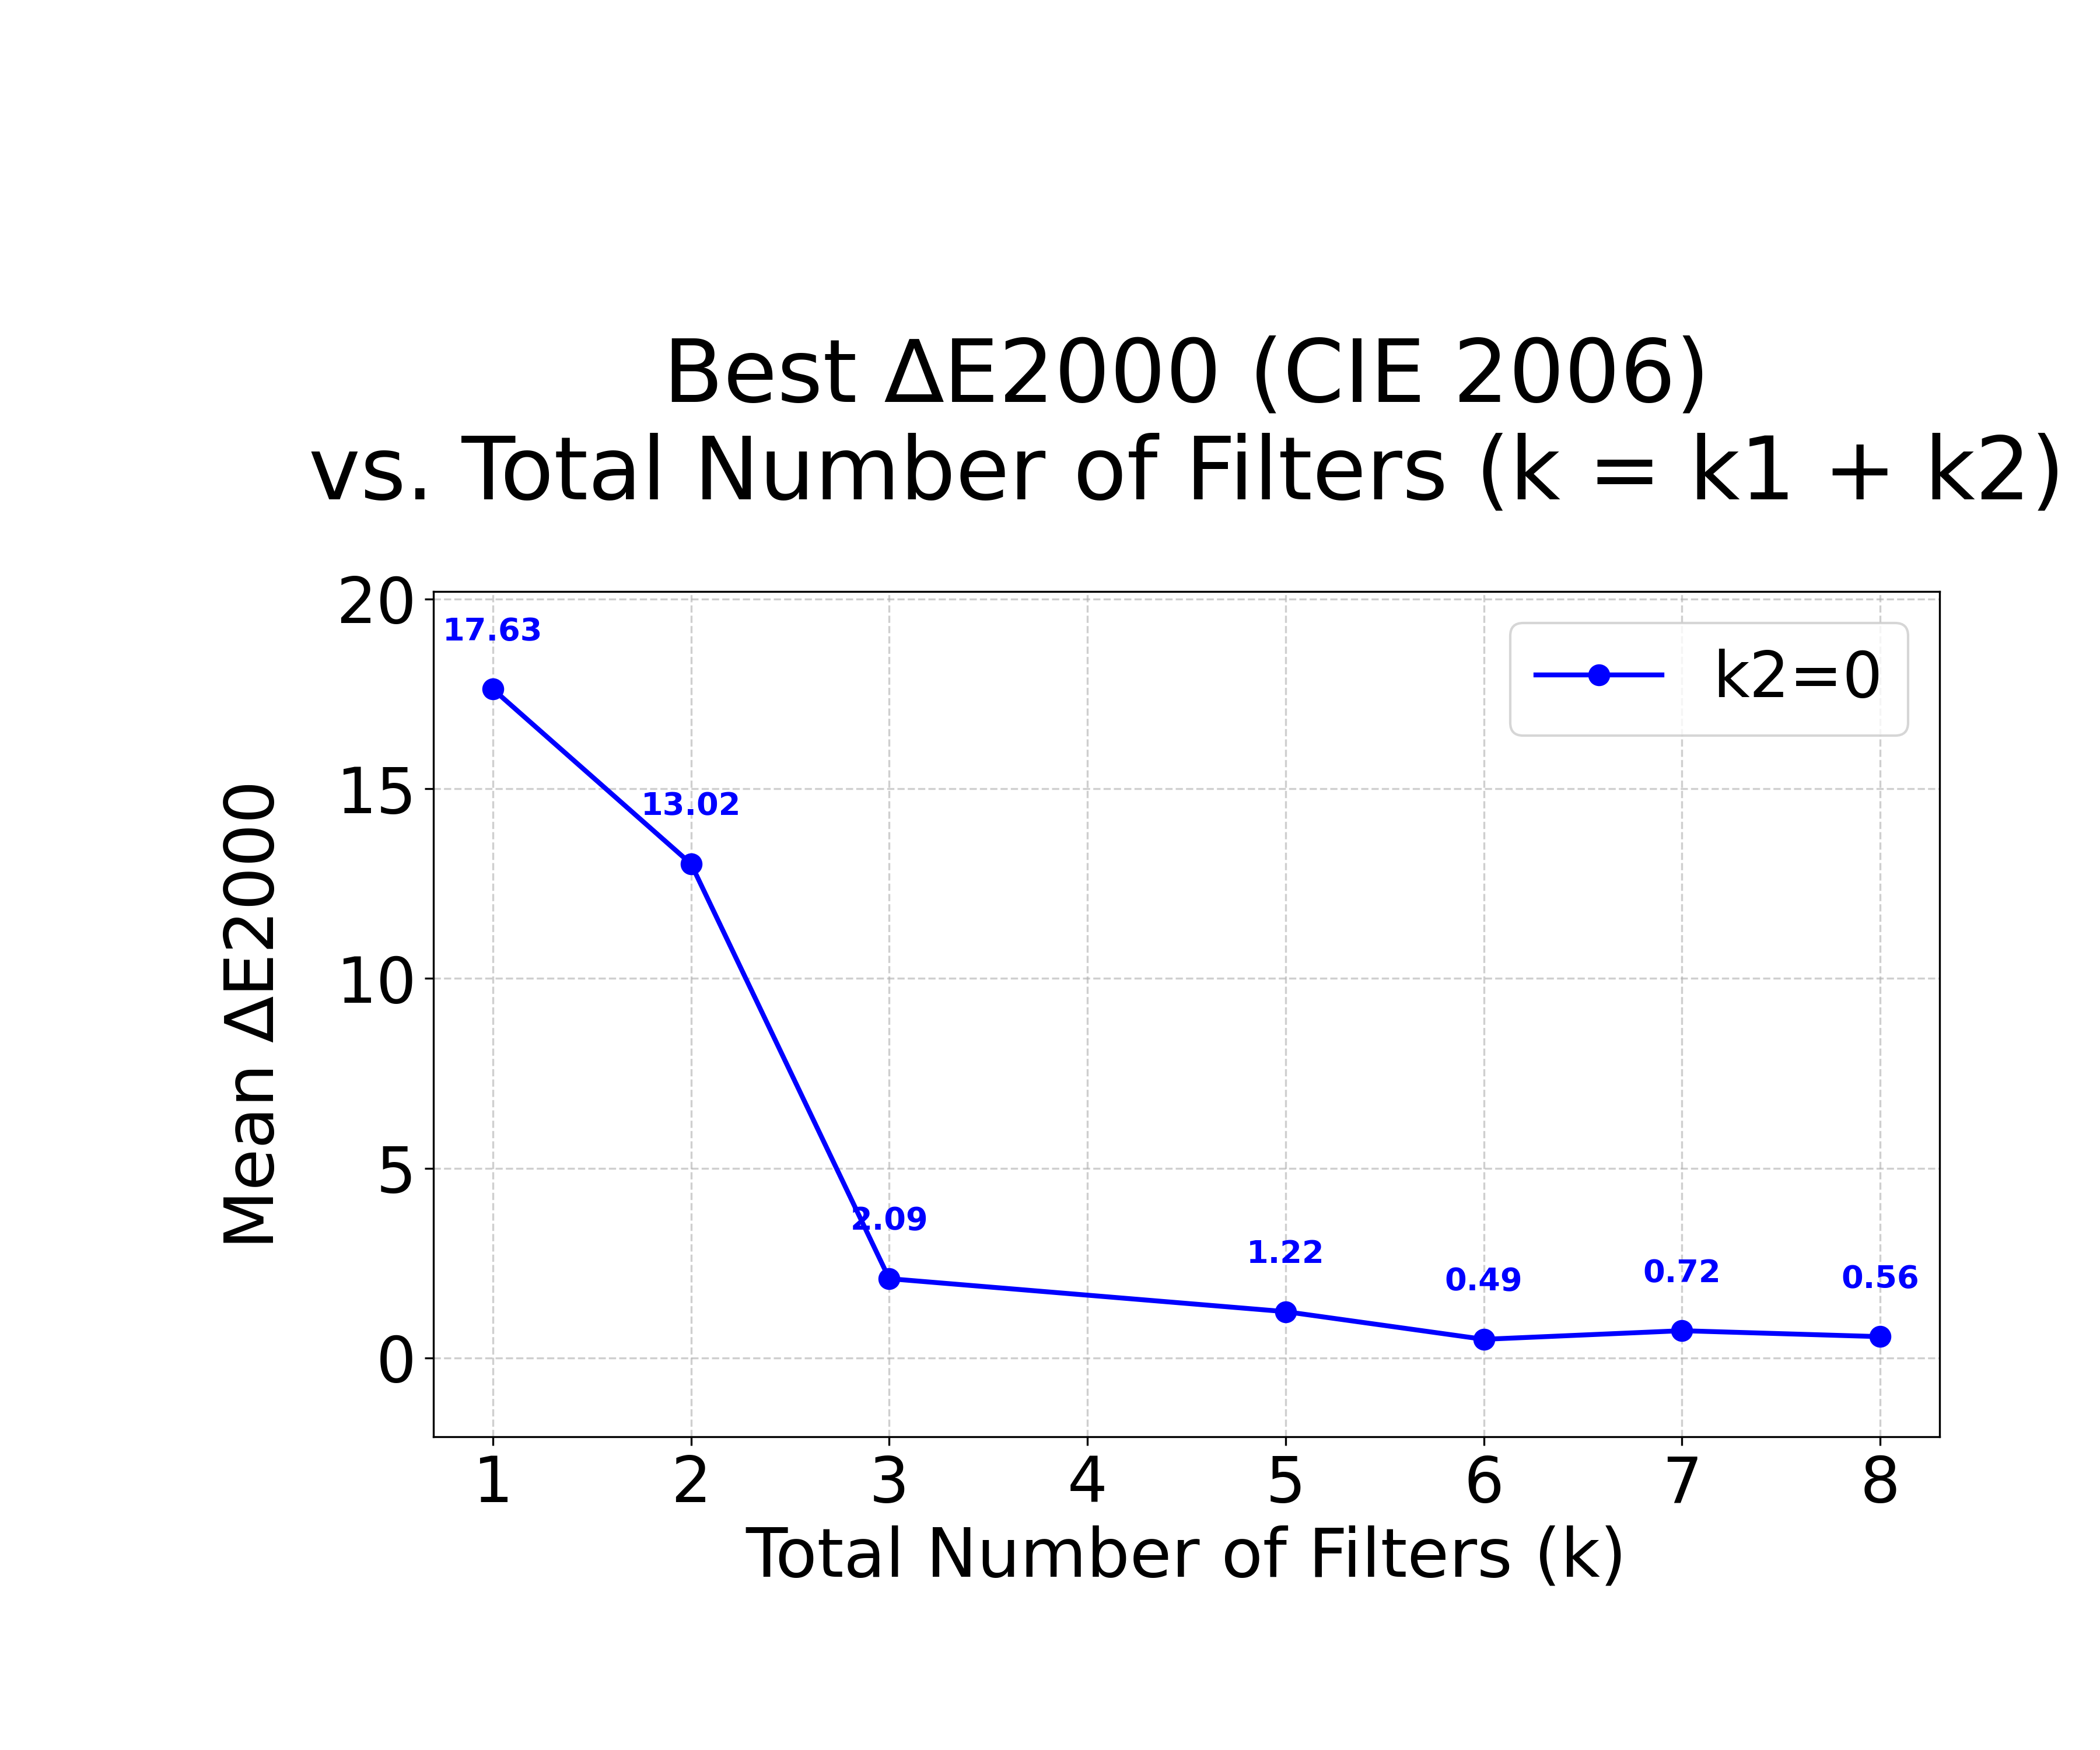
\includegraphics[width=.55\linewidth]{media/deltaE_vs_k_mse10d.png}
    \caption{$\dE$ for $k \in \{1,2...8\}$ for the 10 degree observer}
\end{subfigure}%
\begin{subfigure}{.34\linewidth}
    \centering
    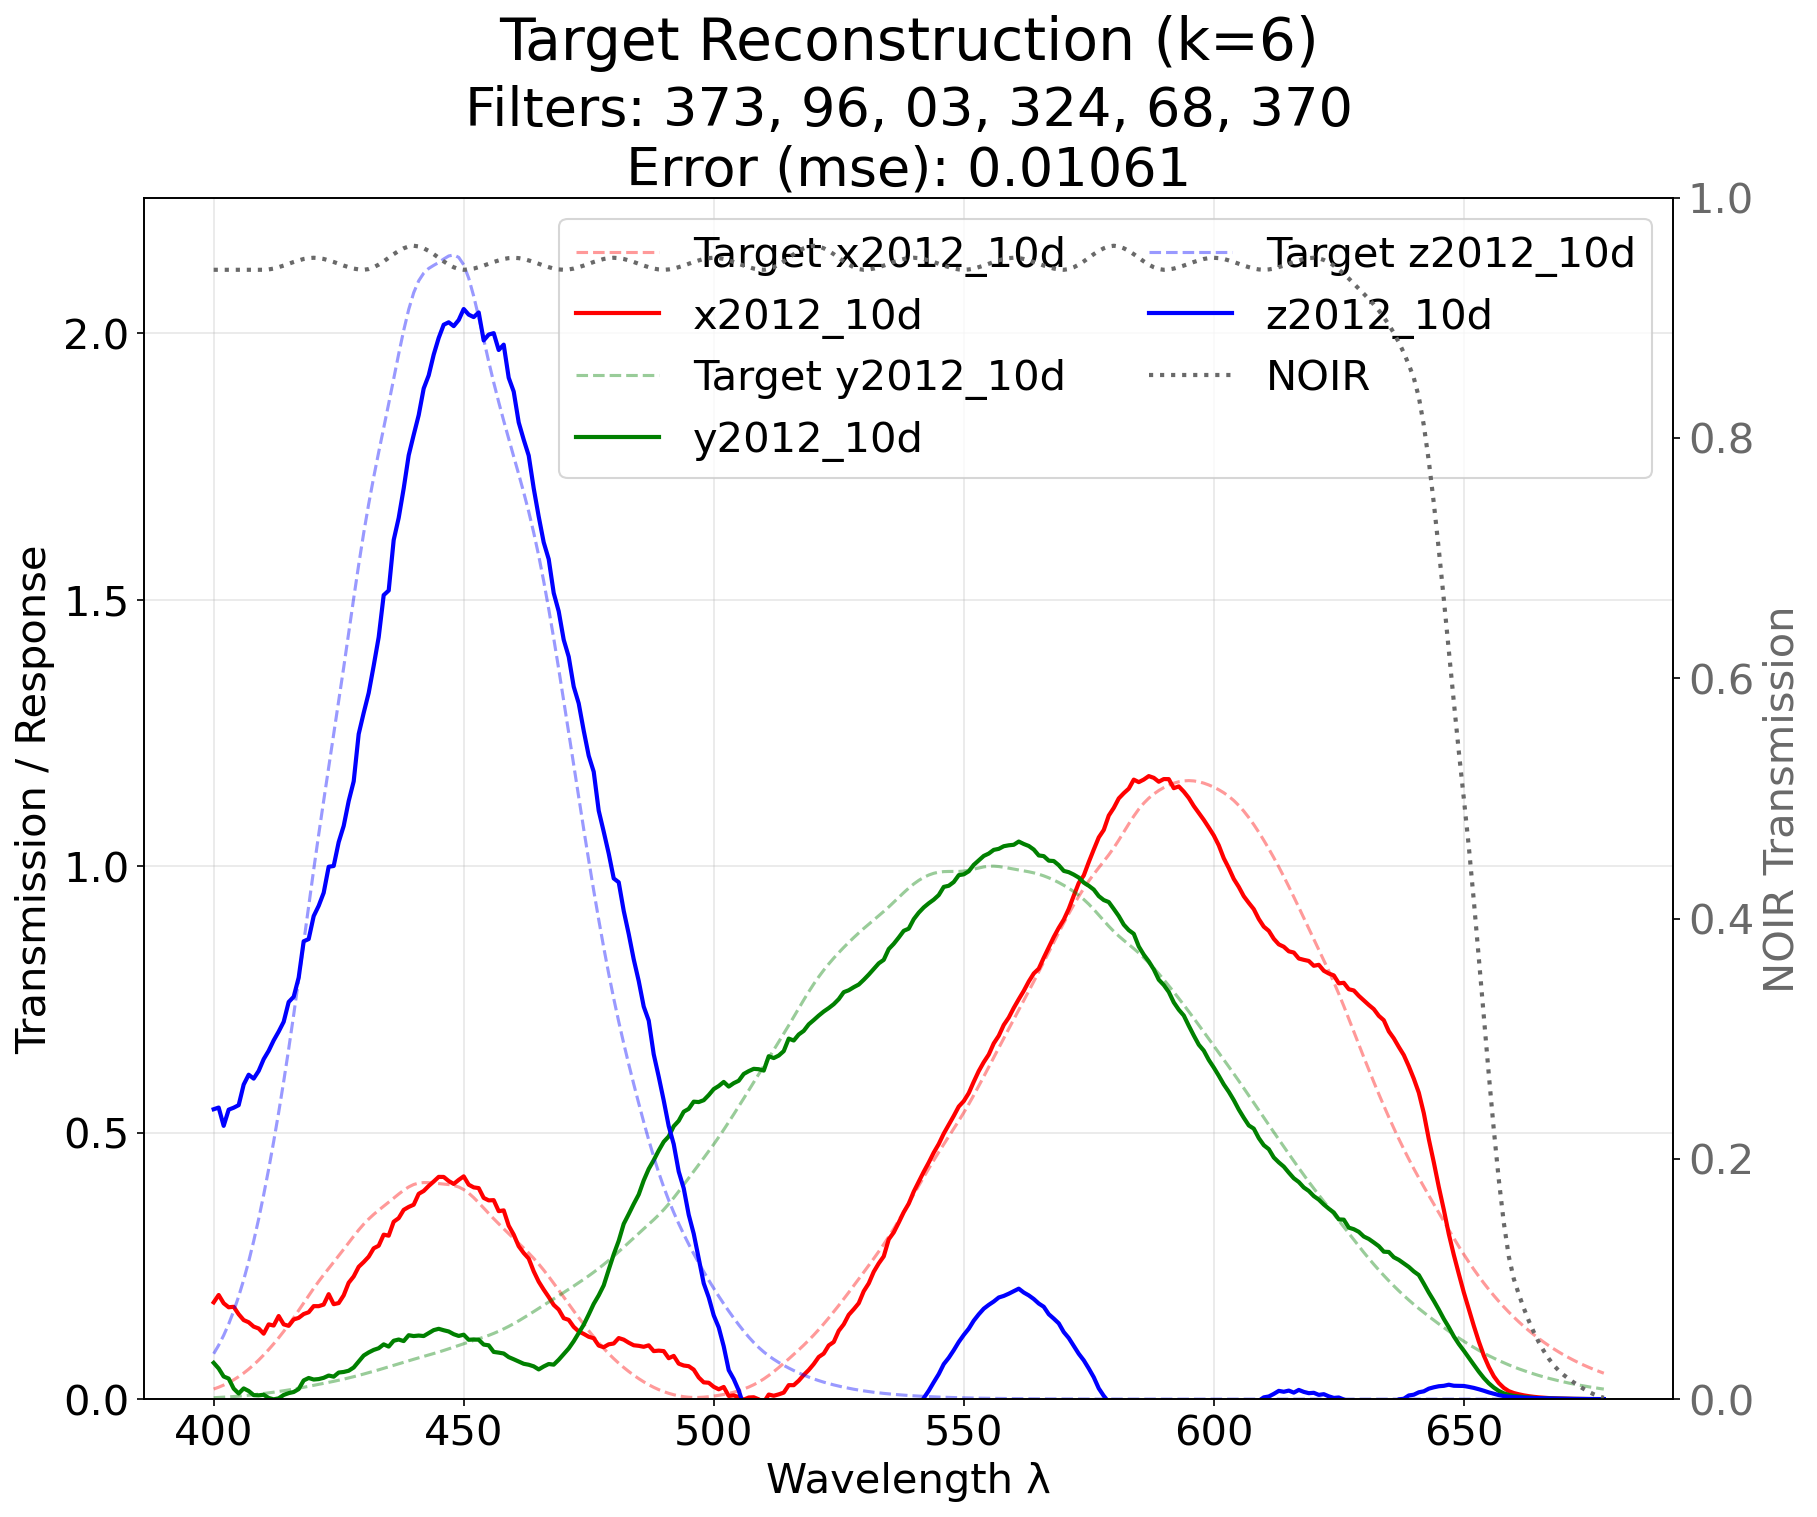
\includegraphics[width=\linewidth]{media/top1_spectra_10d.png}
    \caption{Best Spectral Reconstruction}
\end{subfigure}
\caption{Lab setup for image capture, with deconstructed camera}
\label{fig:10Degrees}
\end{figure}

\section{Algorithm Comparison}

In this section, we analyze the best MSE and $\dE$ for the brute force and PCA algorithms, in the simulated Rosco Supergel set. 
We see that counterintuitively, the best $\dE$ performances are found at the $k_1=3$ and $k_1=4$, $k_2=2$ filter selectors. 
Additionally, we note that the performance is not monotonically decreasing due to the difficulties of the filter selection problem, but again, these $\dE$ metrics are below the just noticeable difference of 1, and thus we note that the simulated reconstructions are fairly indistinguishable from ground truth. 

\begin{table}[H]
    \centering
    \begin{tabular}{llrrrr}
    \toprule
     &  & \multicolumn{2}{r}{Best MSE} & \multicolumn{2}{r}{Best $\dE$} \\
     & Strategy & Brute Force & PCA & Brute Force & PCA \\
    N & N2 &  &  &  &  \\
    \midrule
    \multirow[t]{3}{*}{1} & 0 & 0.1904 & 0.2003 & 20.8603 & 17.7365 \\
      & 1 & 0.1432 & 0.0500 & 12.7010 & 12.6795 \\
      & 2 & 0.0263 & 0.0205 & 7.9875 & 4.6905 \\
    \cline{1-6}
    \multirow[t]{3}{*}{2} & 0 & 0.0489 & 0.0791 & 13.1686 & 13.5027 \\
      & 1 & 0.0392 & 0.0272 & 9.8836 & 6.9481 \\
      & 2 & 0.0188 & 0.0117 & 1.1743 & 1.8973 \\
    \cline{1-6}
    \multirow[t]{3}{*}{3} & 0 & 0.0219 & 0.0457 & 5.4475 & 2.8156 \\
      & 1 & 0.0220 & 0.0117 & 5.3174 & 1.8973 \\
      & 2 & 0.0089 & 0.0037 & 1.5786 & 0.5551 \\
    \cline{1-6}
    \multirow[t]{3}{*}{4} & 0 & 0.0063 & 0.0318 & 1.9277 & 1.6631 \\
      & 1 & 0.0229 & 0.0062 & 1.7381 & 0.9180 \\
      & 2 & 0.0033 & 0.0025 & 0.5718 & 0.3909 \\
    \cline{1-6}
    \multirow[t]{3}{*}{5} & 0 & 0.0034 & 0.0197 & 0.9064 & 0.5701 \\
      & 1 & 0.0108 & 0.0047 & 4.7085 & 0.7234 \\
      & 2 & 0.0021 & 0.0018 & 0.5258 & 0.4879 \\
    \cline{1-6}
    \multirow[t]{3}{*}{6} & 0 & 0.0021 & 0.0146 & 0.4550 & 0.6770 \\
      & 1 & 0.0033 & 0.0044 & 0.6592 & 0.6900 \\
      & 2 & 0.0018 & 0.0015 & 0.4961 & 0.4676 \\
    \cline{1-6}
    \bottomrule
    \end{tabular}
    \caption{Minimum MSE and $\Delta E$ Comparison: PCA vs. Brute Force}
    \label{tab:mse_deltae_comparison}
\end{table}


\subsection{Noise Model Analysis}

For analysis of the noisiness of our capture, we switch from the MSE loss function to the MSE_noisy loss function, and we compare the results with increments in the photons parameter. 
For this analysis, we increment along the $k_1$ parameter amongst $k_1 \in \{2,4,6\}$, fixing $k_2=2$. 
The difference in $\dE$ performance using the noise model is significantly larger due to the worse reconstruction quality attained by adding noise to the loss function.
Hence, $\dE$ attained with $k=4 (k_1=2,k_2=2)$ filters never decreases past 14. 

\begin{center}
    \centering
    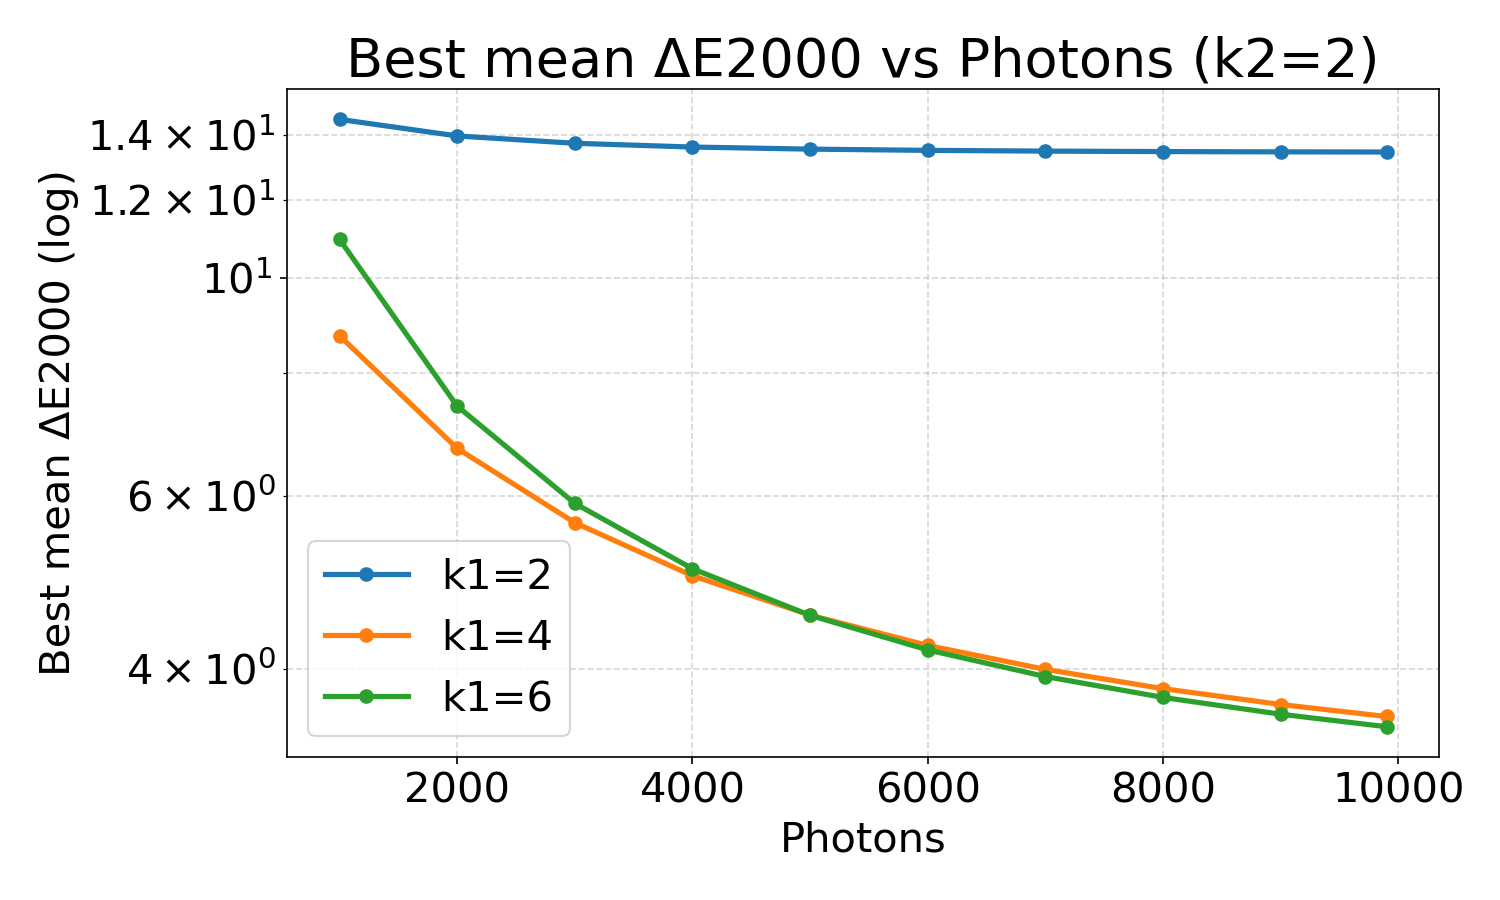
\includegraphics[width=.75\linewidth]{media/photons_sweep_deltaE_20260528_210811.png}
    \captionof{figure}{Best $\dE$ as a function of Photons}
\end{center}

The noise model is not directly used in our filter selection process, but informs our understanding of filter wheel dynamics and shutter speed. 
We also recognize the detrimental effect of poor lighting on our captures, and aim to increase exposure time in low-lighting environments.


\section{Physical Camera with Rosco Supergel Set}

For the initial evaluation of our physical camera stack, we stage an environment under the same Lilliput \cite{UtopiaCamLiliput} illuminant in a lab environment. 
We position the illuminant about 2 meters above the scene to tune the intensity of light into the camera aperture, and place our camera (removed from the housing) on a tripod, aimed at the stage. 

\begin{center}

\end{center}

\begin{figure}[H]
\centering
\begin{subfigure}{.64\linewidth}
    \centering
    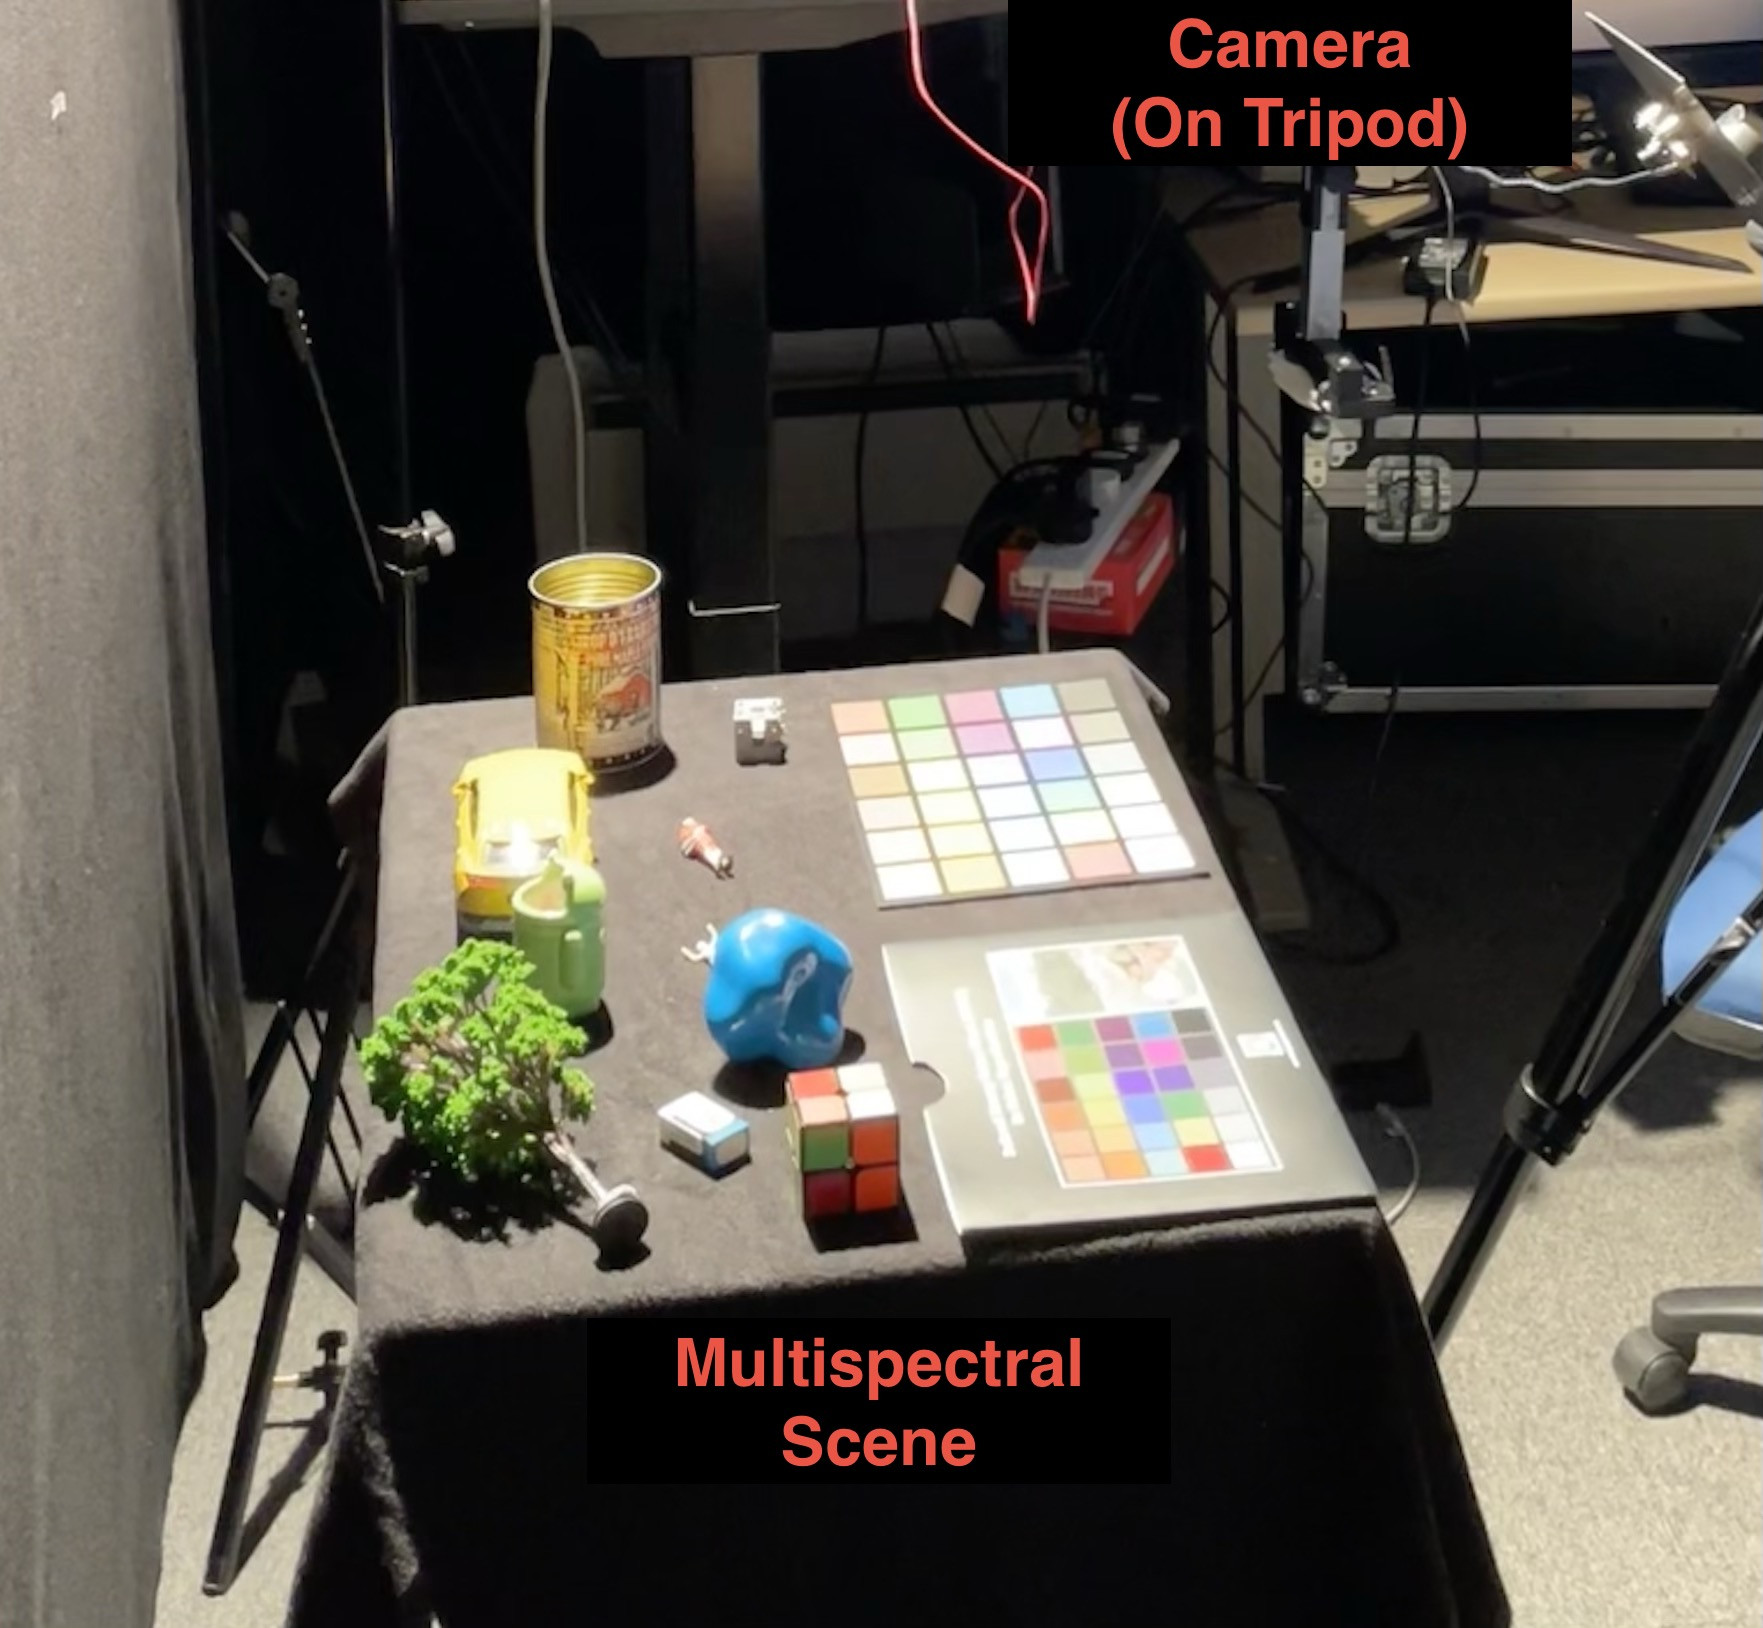
\includegraphics[width=.55\linewidth]{media/spectralLabMarkup.jpeg}
    \caption{Camera on tripod in lab, side angle}
\end{subfigure}%
\begin{subfigure}{.34\linewidth}
    \centering
    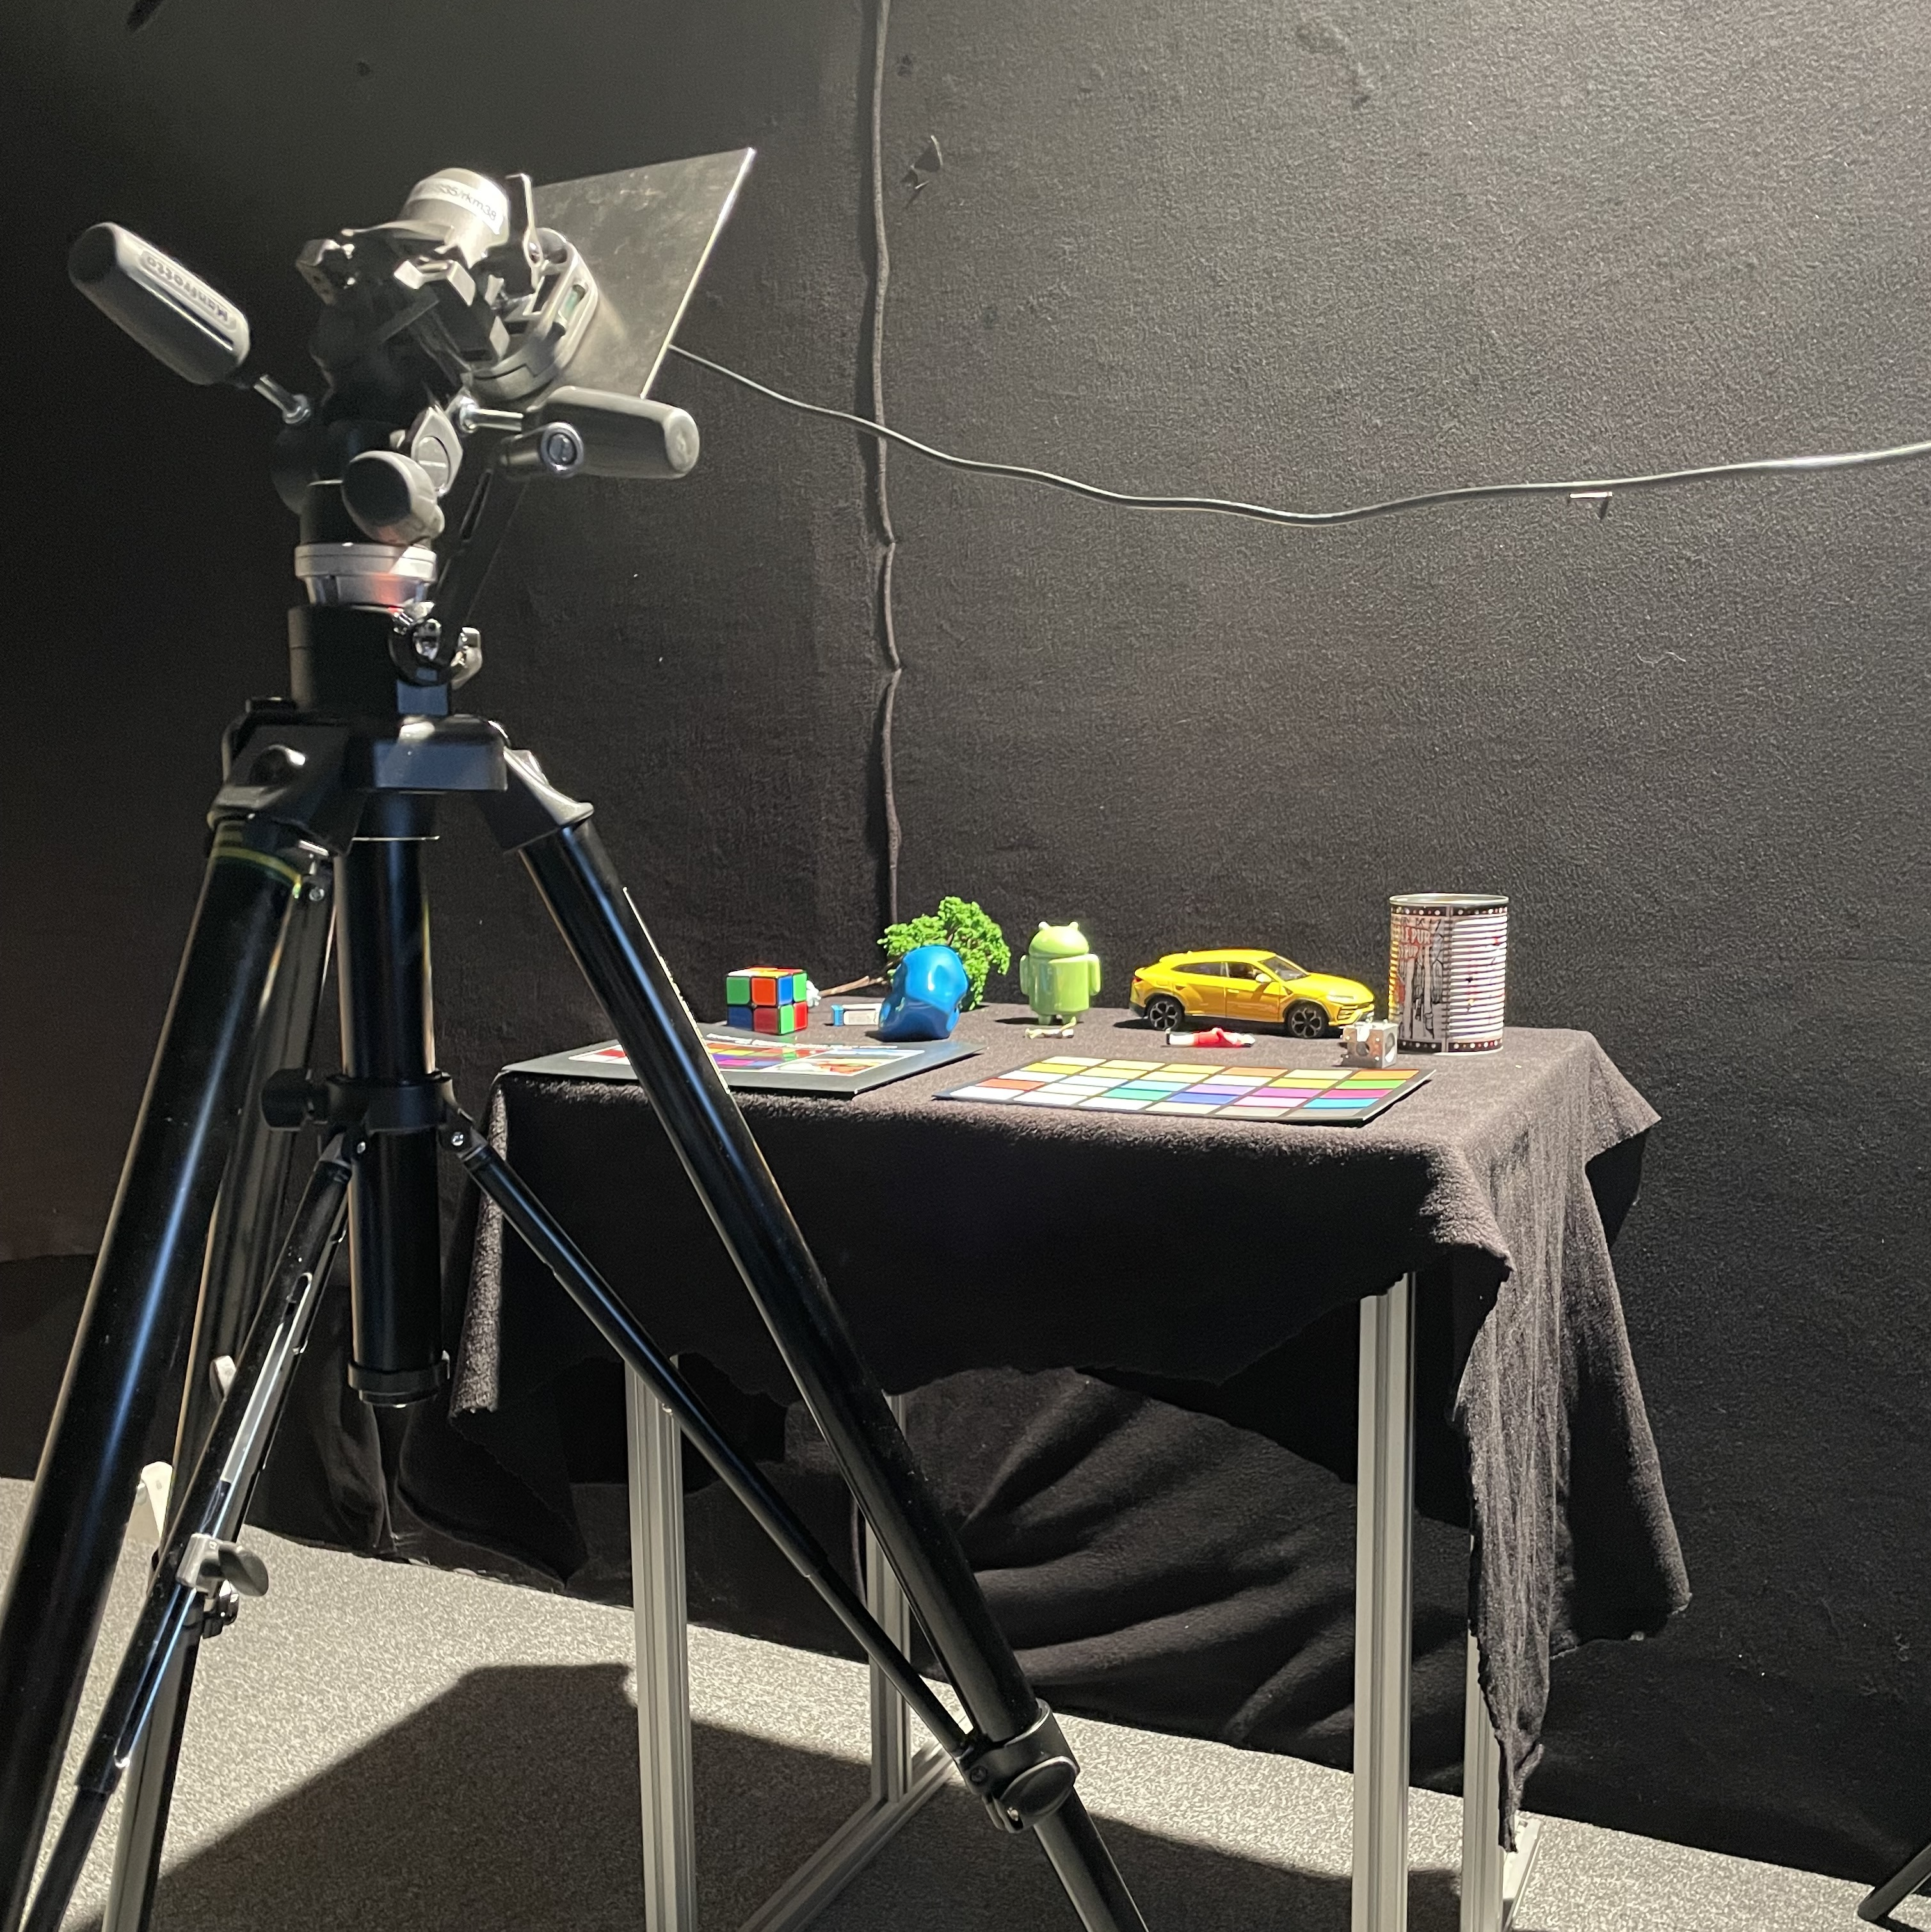
\includegraphics[width=\linewidth]{media/spectralLabMarkupStage.jpeg}
    \caption{Camera on tripod, rear angle}
\end{subfigure}
\caption{Lab setup for image capture, with deconstructed camera}
\label{fig:spectralLabMark}
\end{figure}

Then, we test the recommended best performing filter combinations against a multispectral scene including a PMC in a lab environment, using the Rosco Supergel set of filters. 

We then take the best prescribed reconstructions for the $k_1=4$ and $k_1=5$ reconstructions to test our methodology. 

\begin{center}
    \centering
    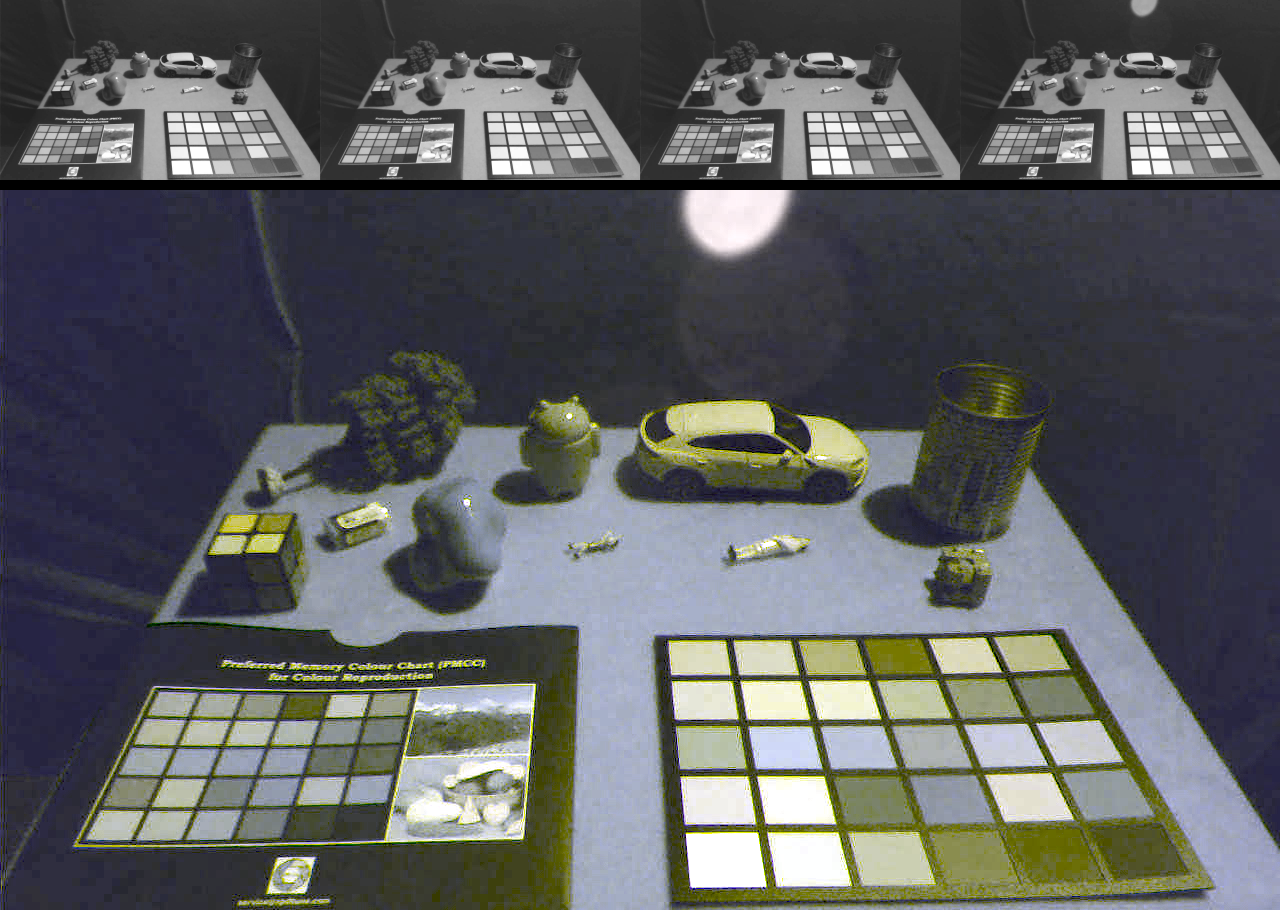
\includegraphics[width=.75\linewidth]{media/k1_4_recon.png}
    \captionof{figure}{$k_1=4$ Photo Lab Reconstruction with component captures above}
\end{center}

Qualitatively, we see that these solutions do not provide perfect reconstructions, and the intensity of some of the hues is dulled. 
For a more quantitative analysis, we utilize the spectrophotometer in this same lab environment \ref{ref:spectrophotometer} and compute the ground truth $x$ and $y$ values. 
Then, we can use the same methodology as the simulated pipeline to compute $\dE$. 

Here, we have the solution for the $k_1=5$ 

\begin{center}
    \centering
    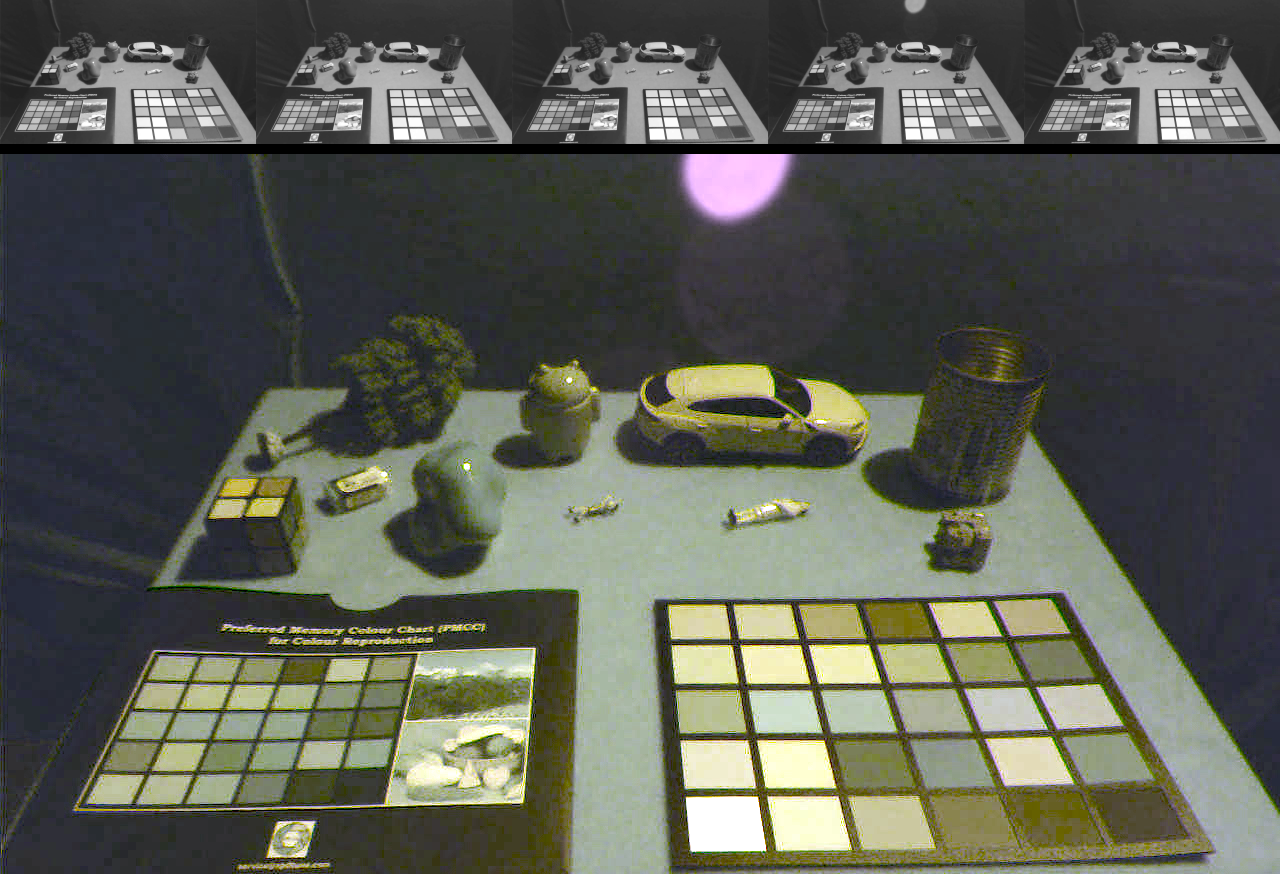
\includegraphics[width=.75\linewidth]{media/k1_5_recon.png}
    \captionof{figure}{$k_1=5$ Photo Lab Reconstruction with component captures above}
\end{center}

\iffalse
\section{Physical Camera Photo Results}

We demonstrate use of our physical camera in non-laboratory settings. 
Here, we have a photo of ____, reconstructed with a filter wheel 
\begin{figure}[H]
\centering
\begin{subfigure}{.49\linewidth}
    \centering
    
\includegraphics[width=\linewidth]{media/placeholder.jpg}
    \caption{Camera and subject taking image of ____}
\end{subfigure}
\begin{subfigure}{.49\linewidth}
    \centering
    
\includegraphics[width=\linewidth]{media/placeholder.jpg}
    \caption{Reconstruction of ___ image}
\end{subfigure}
\caption{$k=4$ real world capture}
\end{figure}

Another capture is shown below, this time in low lighting environment.

\begin{figure}[H]
\centering
\begin{subfigure}{.49\linewidth}
    \centering
    
\includegraphics[width=\linewidth]{media/placeholder.jpg}
    \caption{Camera and subject taking image of ____}
\end{subfigure}
\begin{subfigure}{.49\linewidth}
    \centering
    
\includegraphics[width=\linewidth]{media/placeholder.jpg}
    \caption{Reconstruction of ___ image}
\end{subfigure}
\caption{$k=4$ real world capture}
\end{figure}

Here, we use a 6 filter wheel to capture the same environment. 

\begin{figure}[H]
\centering
\begin{subfigure}{.49\linewidth}
    \centering
    
\includegraphics[width=\linewidth]{media/placeholder.jpg}
    \caption{Camera and subject taking image of ____}
\end{subfigure}
\begin{subfigure}{.49\linewidth}
    \centering
    
\includegraphics[width=\linewidth]{media/placeholder.jpg}
    \caption{Reconstruction of ___ image}
\end{subfigure}
\caption{$k=6$ real world capture}
\end{figure}
\fi
\setcounter{chapter}{5}
\chapter{Conclusion}
We are able to achieve fairly accurate reconstructions of the XYZ color matching functions with as few as $k=4$ filters, and very high quality reconstructions with $k>5$ filters.
This suggests that a filter wheel system with 6 filters could be sufficient for high-quality color reconstruction. 
However, the system does have drawbacks, such as shutter speed on the order of seconds and the need for a static scene. 


\end{multicols}

\newpage

\addcontentsline{toc}{section}{References}

\bibliography{document.bib} 
\bibliographystyle{ieeetr}
\newpage
\setcounter{chapter}{6}

\section{Appendix}

\subsection{Filter Selection Timing Analysis}

We include the timing records of our filter selection. 
Both routines were run on NVIDIA GPU environment with the Brute Force run pruned to cosine similarity of .95 and able to utilize 8 GPUs. 
Conversely, the PCA algorithm used one GPU for calculation and 8 GPUs only for the augmented steps. 

\begin{table}[htbp]
    \begin{tabular}{llrrrrrr}
    \toprule
    &  & \multicolumn{2}{r}{Base Time (s)} & \multicolumn{2}{r}{Aug Time (s)} & \multicolumn{2}{r}{Total Time (s)} \\
    & Strategy & Brute Force & PCA & Brute Force & PCA & Brute Force & PCA \\
    $k_1$ & $k_2$ &  &  &  &  &  &  \\
    \midrule
    \multirow[t]{3}{*}{1} & 0 & 13.70 & 7.50 & 0.00 & 0.00 & 13.70 & 7.50 \\
    & 1 & 13.70 & 7.50 & 19.23 & 19.98 & 32.93 & 27.48 \\
    & 2 & 13.70 & 7.50 & 20.61 & 20.89 & 34.31 & 28.40 \\
    \cline{1-8}
    \multirow[t]{3}{*}{2} & 0 & 12.58 & 6.80 & 0.00 & 0.00 & 12.58 & 6.80 \\
    & 1 & 12.58 & 6.80 & 20.83 & 20.41 & 33.41 & 27.20 \\
    & 2 & 12.58 & 6.80 & 20.30 & 18.34 & 32.88 & 25.13 \\
    \cline{1-8}
    \multirow[t]{3}{*}{3} & 0 & 13.26 & 5.85 & 0.00 & 0.00 & 13.26 & 5.85 \\
    & 1 & 13.26 & 5.85 & 18.26 & 20.08 & 31.52 & 25.93 \\
    & 2 & 13.26 & 5.85 & 21.61 & 19.95 & 34.87 & 25.80 \\
    \cline{1-8}
    \multirow[t]{3}{*}{4} & 0 & 16.03 & 7.55 & 0.00 & 0.00 & 16.03 & 7.55 \\
    & 1 & 16.03 & 7.55 & 18.69 & 19.39 & 34.71 & 26.94 \\
    & 2 & 16.03 & 7.55 & 19.11 & 18.75 & 35.13 & 26.30 \\
    \cline{1-8}
    \multirow[t]{3}{*}{5} & 0 & 18.88 & 5.80 & 0.00 & 0.00 & 18.88 & 5.80 \\
    & 1 & 18.88 & 5.80 & 19.69 & 19.23 & 38.57 & 25.03 \\
    & 2 & 18.88 & 5.80 & 19.61 & 18.86 & 38.49 & 24.65 \\
    \cline{1-8}
    \multirow[t]{3}{*}{6} & 0 & 33.33 & 6.04 & 0.00 & 0.00 & 33.33 & 6.04 \\
    & 1 & 33.33 & 6.04 & 17.74 & 18.10 & 51.07 & 24.14 \\
    & 2 & 33.33 & 6.04 & 18.54 & 20.12 & 51.87 & 26.15 \\
    \cline{1-8}
    \multirow[t]{3}{*}{7} & 0 & 81.34 & 6.26 & 0.00 & 0.00 & 81.34 & 6.26 \\
    & 1 & 81.34 & 6.26 & 19.17 & 19.45 & 100.51 & 25.71 \\
    & 2 & 81.34 & 6.26 & 19.11 & 19.72 & 100.45 & 25.98 \\
    \cline{1-8}
    \multirow[t]{3}{*}{8} & 0 & 190.31 & 6.55 & 0.00 & 0.00 & 190.31 & 6.55 \\
    & 1 & 190.31 & 6.55 & 20.31 & 20.26 & 210.62 & 26.81 \\
    & 2 & 190.31 & 6.55 & 20.17 & 20.80 & 210.49 & 27.35 \\
    \cline{1-8}
    \bottomrule
    \end{tabular}
    \caption{Timing Comparison: PCA vs. Brute Force, up to $k_1=8$, $k_2=2$}
    \label{tab:timing_comparison}

\end{table}
\newpage
We also include the full loss and $\dE$ results. 
Note that 'Brute Force with Augmentation' considers additional filters to only the top result at $k_1$, and hence can have worse MSE than the PCA solution, which maximizes for orthogonality among filters. 

\begin{table}[htbp]
    \centering
    \begin{tabular}{llrrrr}
    \toprule
     &  & \multicolumn{2}{r}{Best MSE} & \multicolumn{2}{r}{Best $\Delta E$} \\
     & Strategy & Brute Force & PCA & Brute Force & PCA \\
    $k_1$ & $k_2$ &  &  &  &  \\
    \midrule
    \multirow[t]{3}{*}{1} & 0 & 0.1904 & 0.2003 & 20.8603 & 17.7365 \\
      & 1 & 0.1432 & 0.0500 & 12.7010 & 12.6795 \\
      & 2 & 0.0263 & 0.0205 & 7.9875 & 4.6905 \\
    \cline{1-6}
    \multirow[t]{3}{*}{2} & 0 & 0.0489 & 0.0791 & 13.1686 & 13.5027 \\
      & 1 & 0.0392 & 0.0272 & 9.8836 & 6.9481 \\
      & 2 & 0.0188 & 0.0117 & 1.1743 & 1.8973 \\
    \cline{1-6}
    \multirow[t]{3}{*}{3} & 0 & 0.0219 & 0.0457 & 5.4475 & 2.8156 \\
      & 1 & 0.0220 & 0.0117 & 5.3174 & 1.8973 \\
      & 2 & 0.0089 & 0.0037 & 1.5786 & 0.5551 \\
    \cline{1-6}
    \multirow[t]{3}{*}{4} & 0 & 0.0063 & 0.0318 & 1.9277 & 1.6631 \\
      & 1 & 0.0229 & 0.0062 & 1.7381 & 0.9180 \\
      & 2 & 0.0033 & 0.0025 & 0.5718 & 0.3909 \\
    \cline{1-6}
    \multirow[t]{3}{*}{5} & 0 & 0.0034 & 0.0197 & 0.9064 & 0.5701 \\
      & 1 & 0.0108 & 0.0047 & 4.7085 & 0.7234 \\
      & 2 & 0.0021 & 0.0018 & 0.5258 & 0.4879 \\
    \cline{1-6}
    \multirow[t]{3}{*}{6} & 0 & 0.0021 & 0.0146 & 0.4550 & 0.6770 \\
      & 1 & 0.0033 & 0.0044 & 0.6592 & 0.6900 \\
      & 2 & 0.0018 & 0.0015 & 0.4961 & 0.4676 \\
    \cline{1-6}
    \bottomrule
    \end{tabular}
    \caption{Minimum MSE and $\Delta E$ Comparison: PCA vs. Brute Force, up to $k_1=6$, $k_2=2$}
    \label{tab:mse_deltae_comparison}
\end{table}

\subsection{Code Snippets}
We include code snippets from some of the algorithms outlined above and some of the infrastructure necessary for completing this research. 
The repository is available at this link: \href{https://github.com/kylefram/MultispectralCamera/tree/main}{https://github.com/kylefram/MultispectralCamera/tree/main}

\subsection{CAVE Dataset}

%%% TODO
%%% CHANGE TO GROUND TRUTH -> OTHERS instead of pairs with ground truths

We include images from the CAVE dataset, rendered under various $k \in \{2,3,4,8\}$ values. 
We consider the set of simulations including an IR-cut filter, and filters selected with the brute force methodology, having $k_2=0$.
Because the $k=8$ solution takes some time to brute force, we use a cosine similarity function to prune the filters to a set of 45, which reduces reconstruction quality and increases the differences in $\dE$ across renders. 

\begin{figure}[H]
\centering
\begin{subfigure}{.49\linewidth}
    \centering
    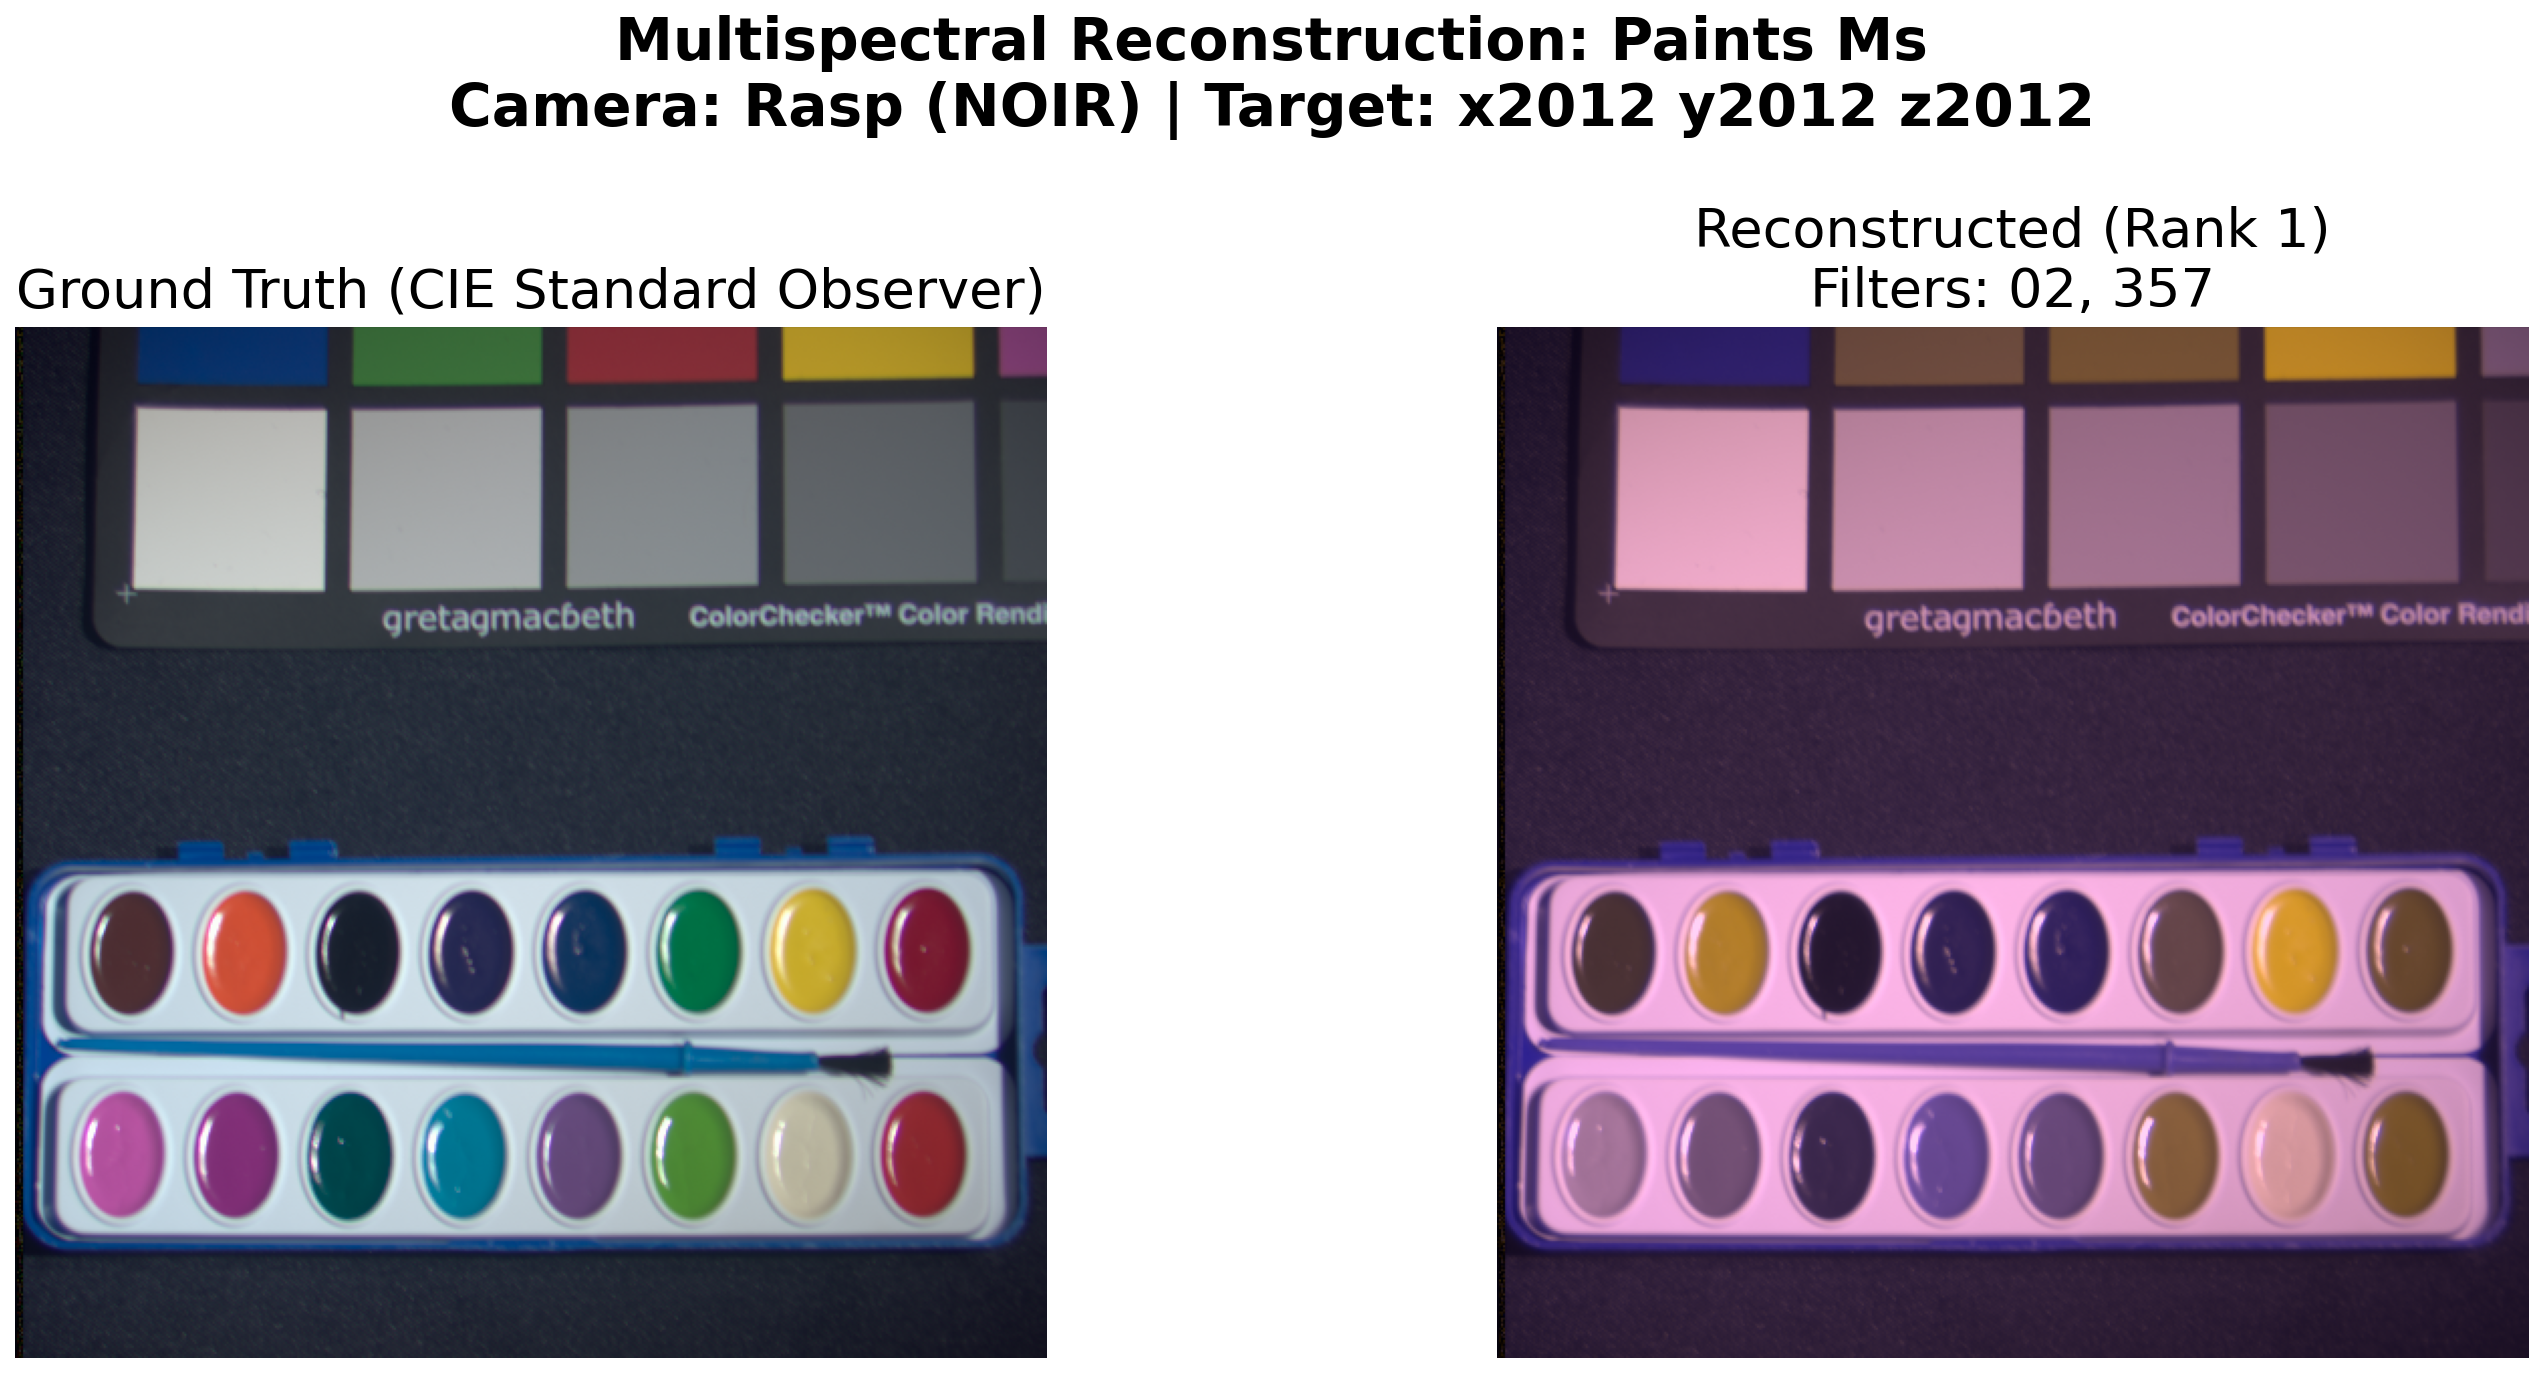
\includegraphics[width=\linewidth]{media/cave_appendix/k2paints.png}
    \caption{$k=2$, $\dE$=13.17}
\end{subfigure}
\begin{subfigure}{.49\linewidth}
    \centering
    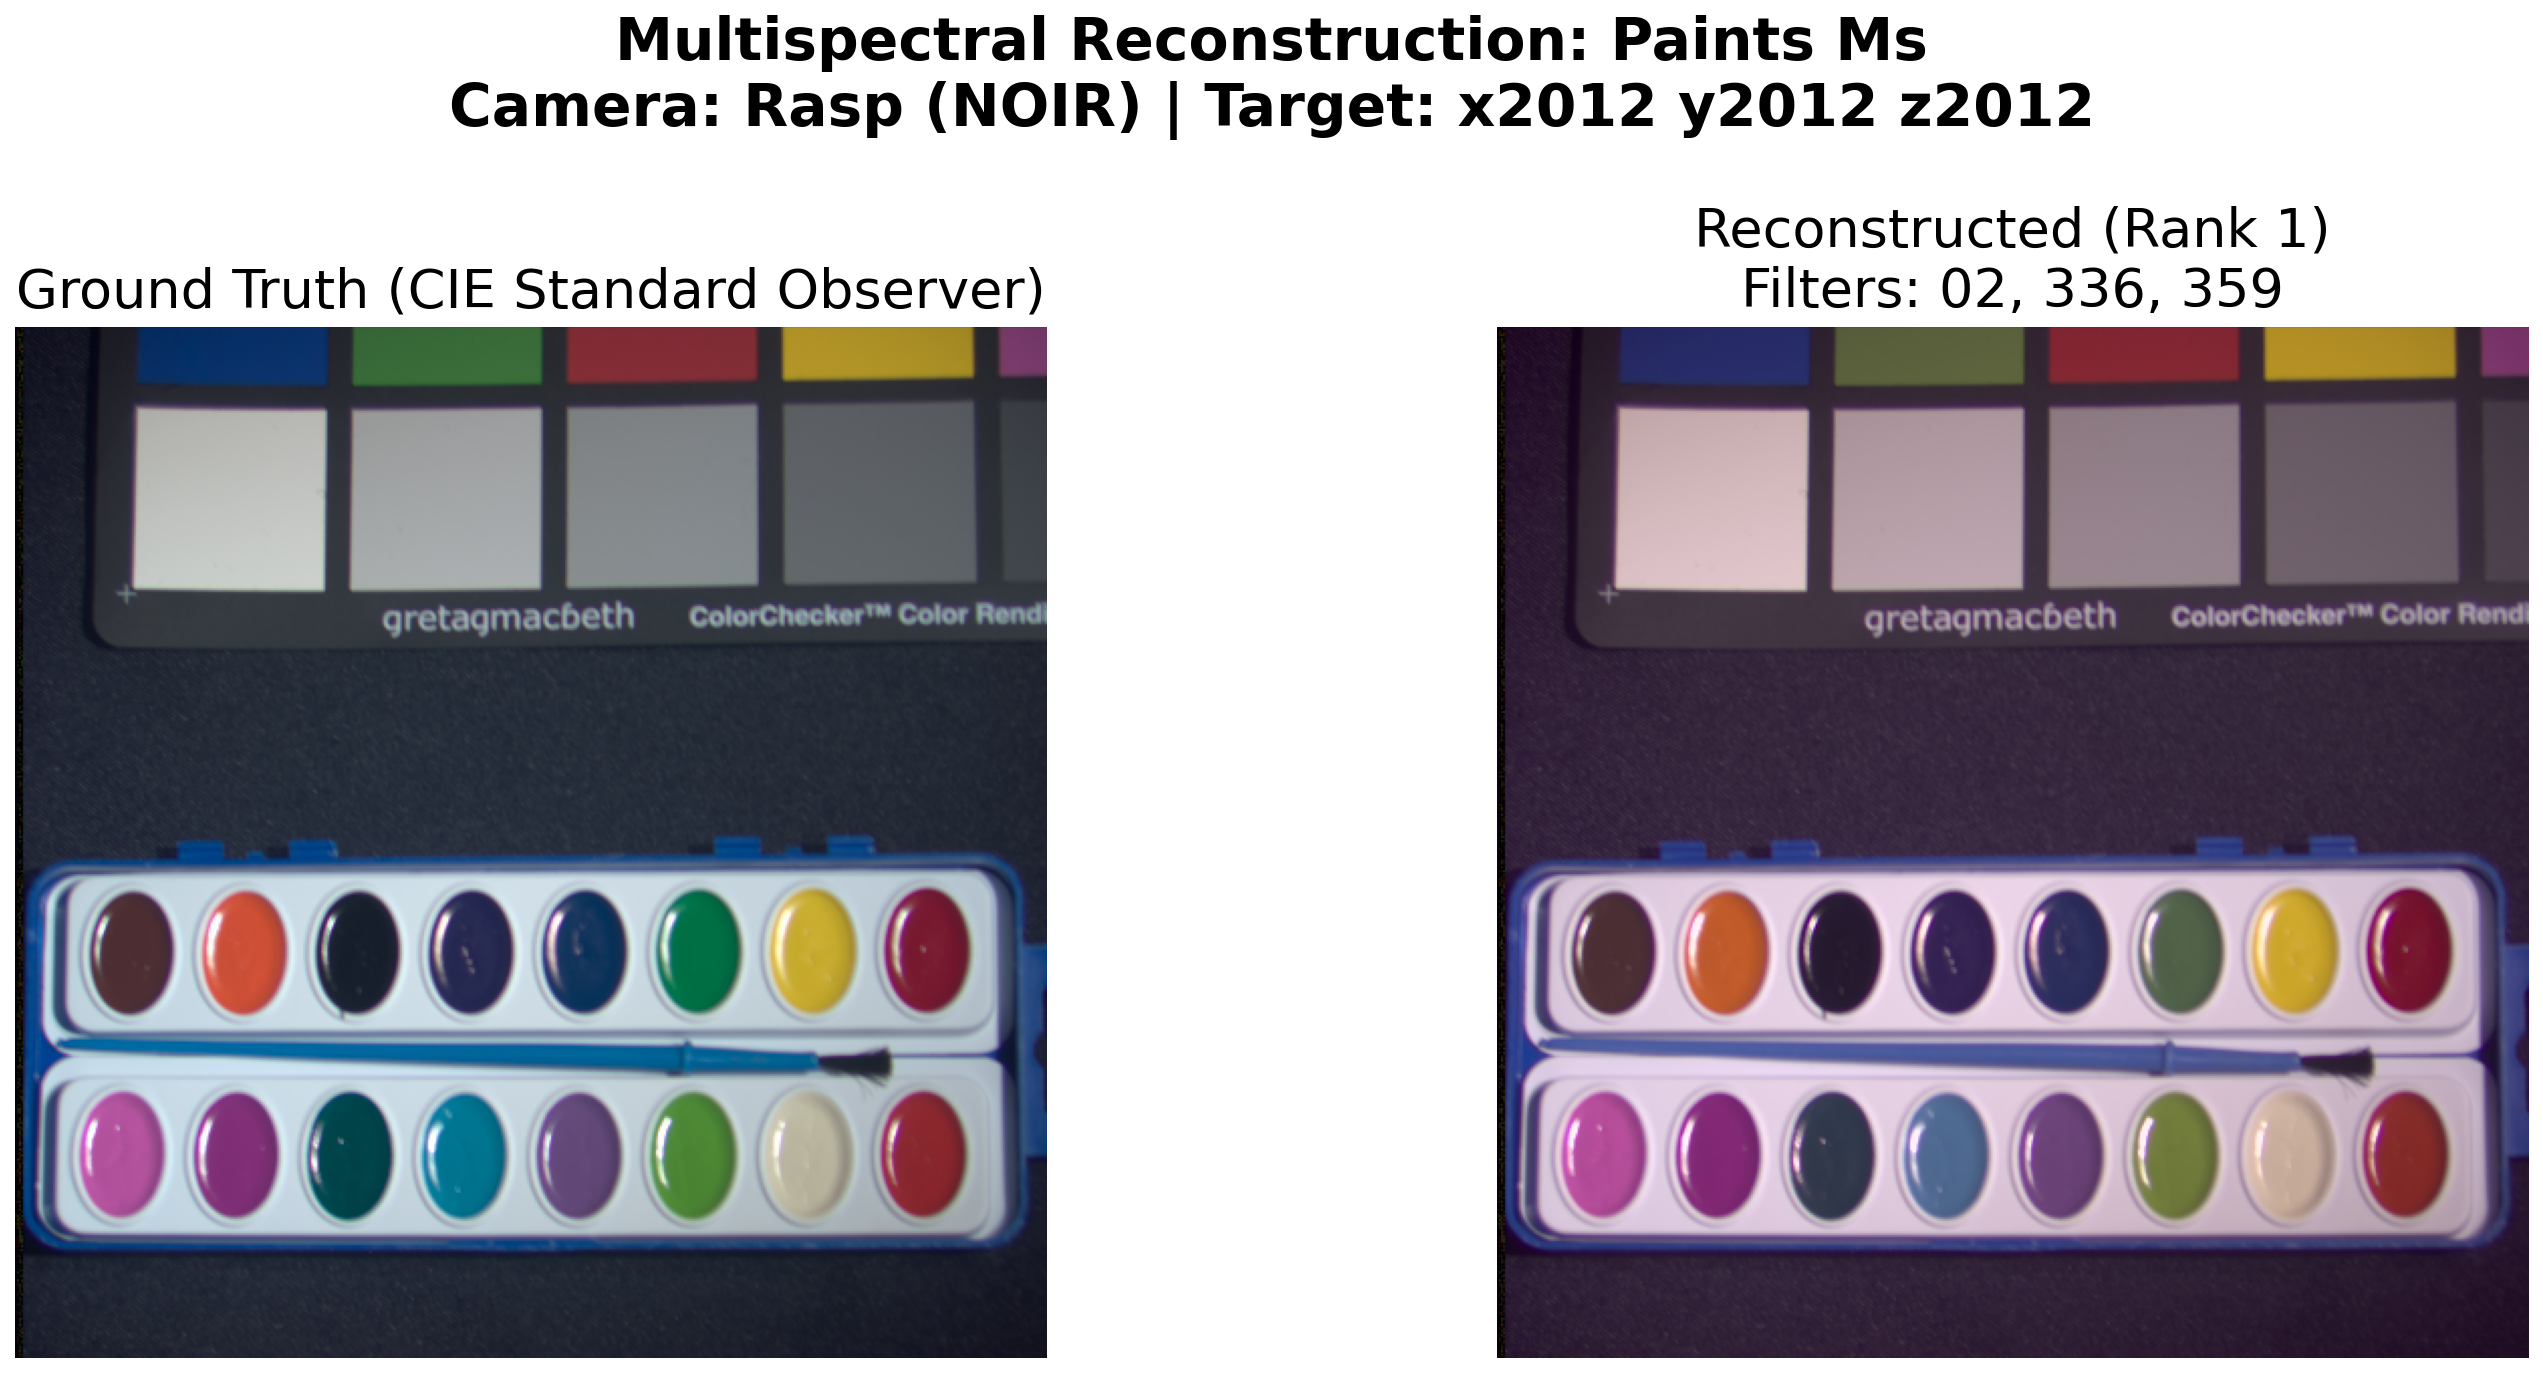
\includegraphics[width=\linewidth]{media/cave_appendix/k3paints.png}
    \caption{$k=3$, $\dE$=5.45}
\end{subfigure}
\begin{subfigure}{.49\linewidth}
    \centering
    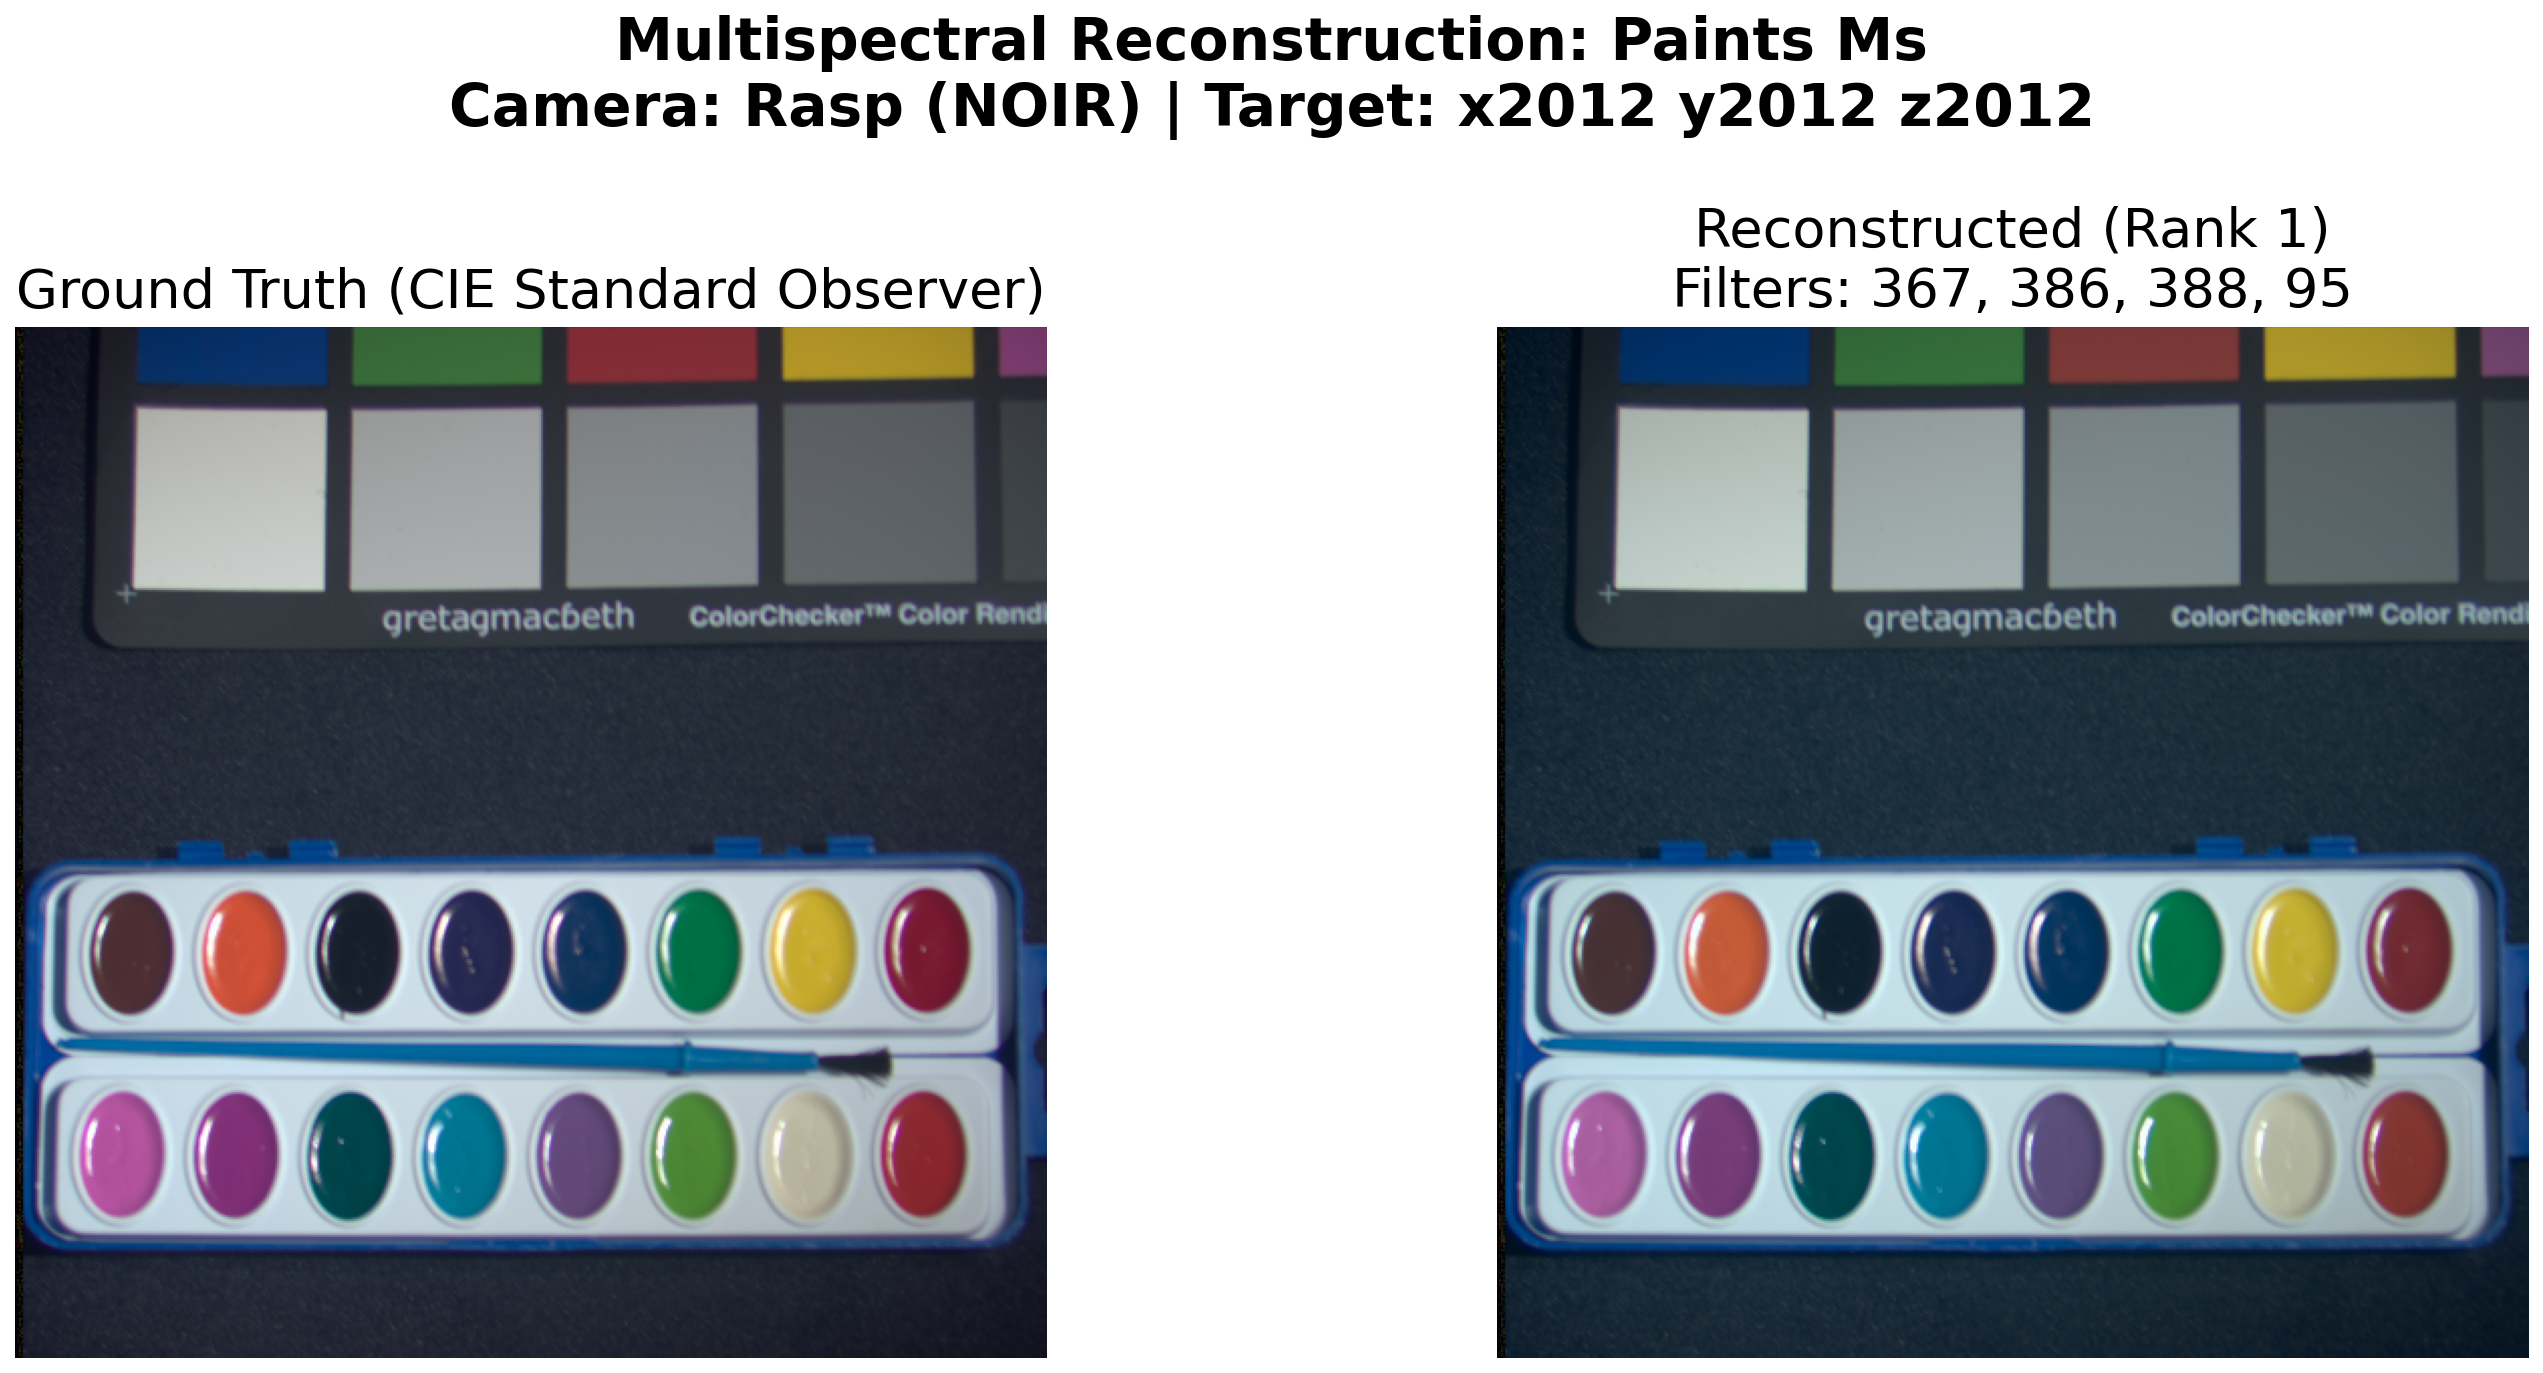
\includegraphics[width=\linewidth]{media/cave_appendix/k4paints.png}
    \caption{$k=4$, $\dE$=1.93}
\end{subfigure}
\begin{subfigure}{.49\linewidth}
    \centering
    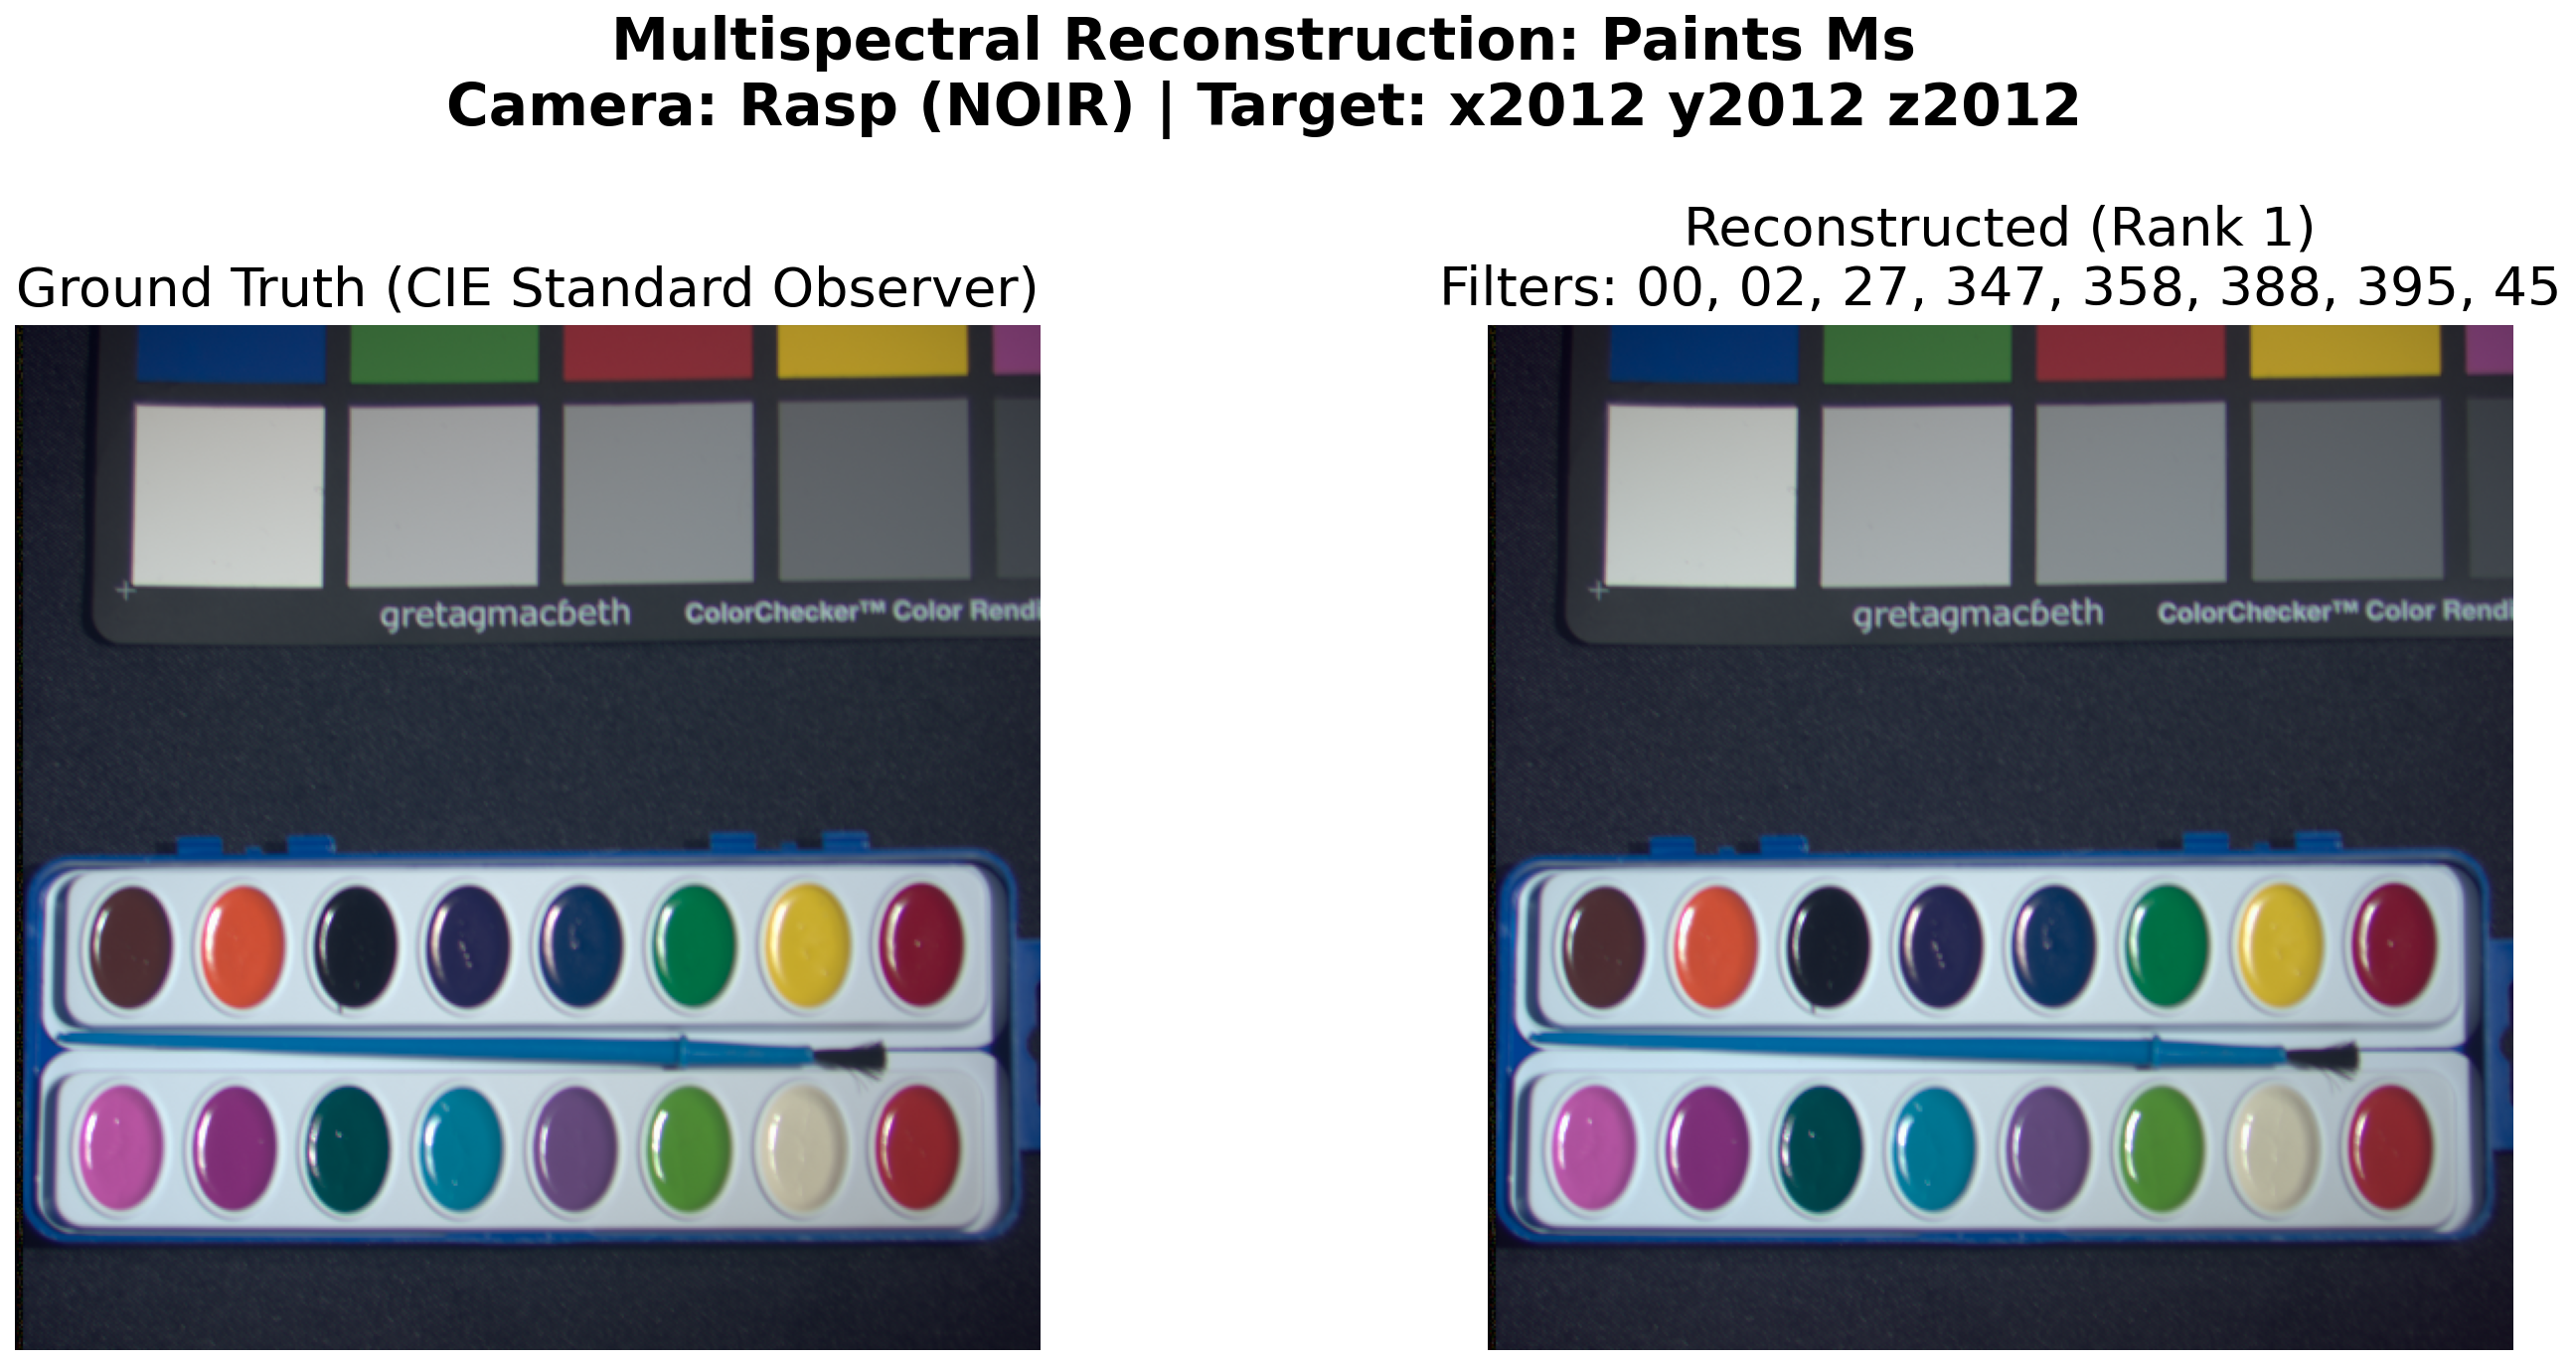
\includegraphics[width=\linewidth]{media/cave_appendix/k8paints.png}
    \caption{$k=8$, $\dE$=.61}
\end{subfigure}
\caption{CAVE Renders of Paints Multispectral Dataset, With Macbeth $\dE$}
\end{figure}

\begin{figure}[H]
\centering
\begin{subfigure}{.49\linewidth}
    \centering
    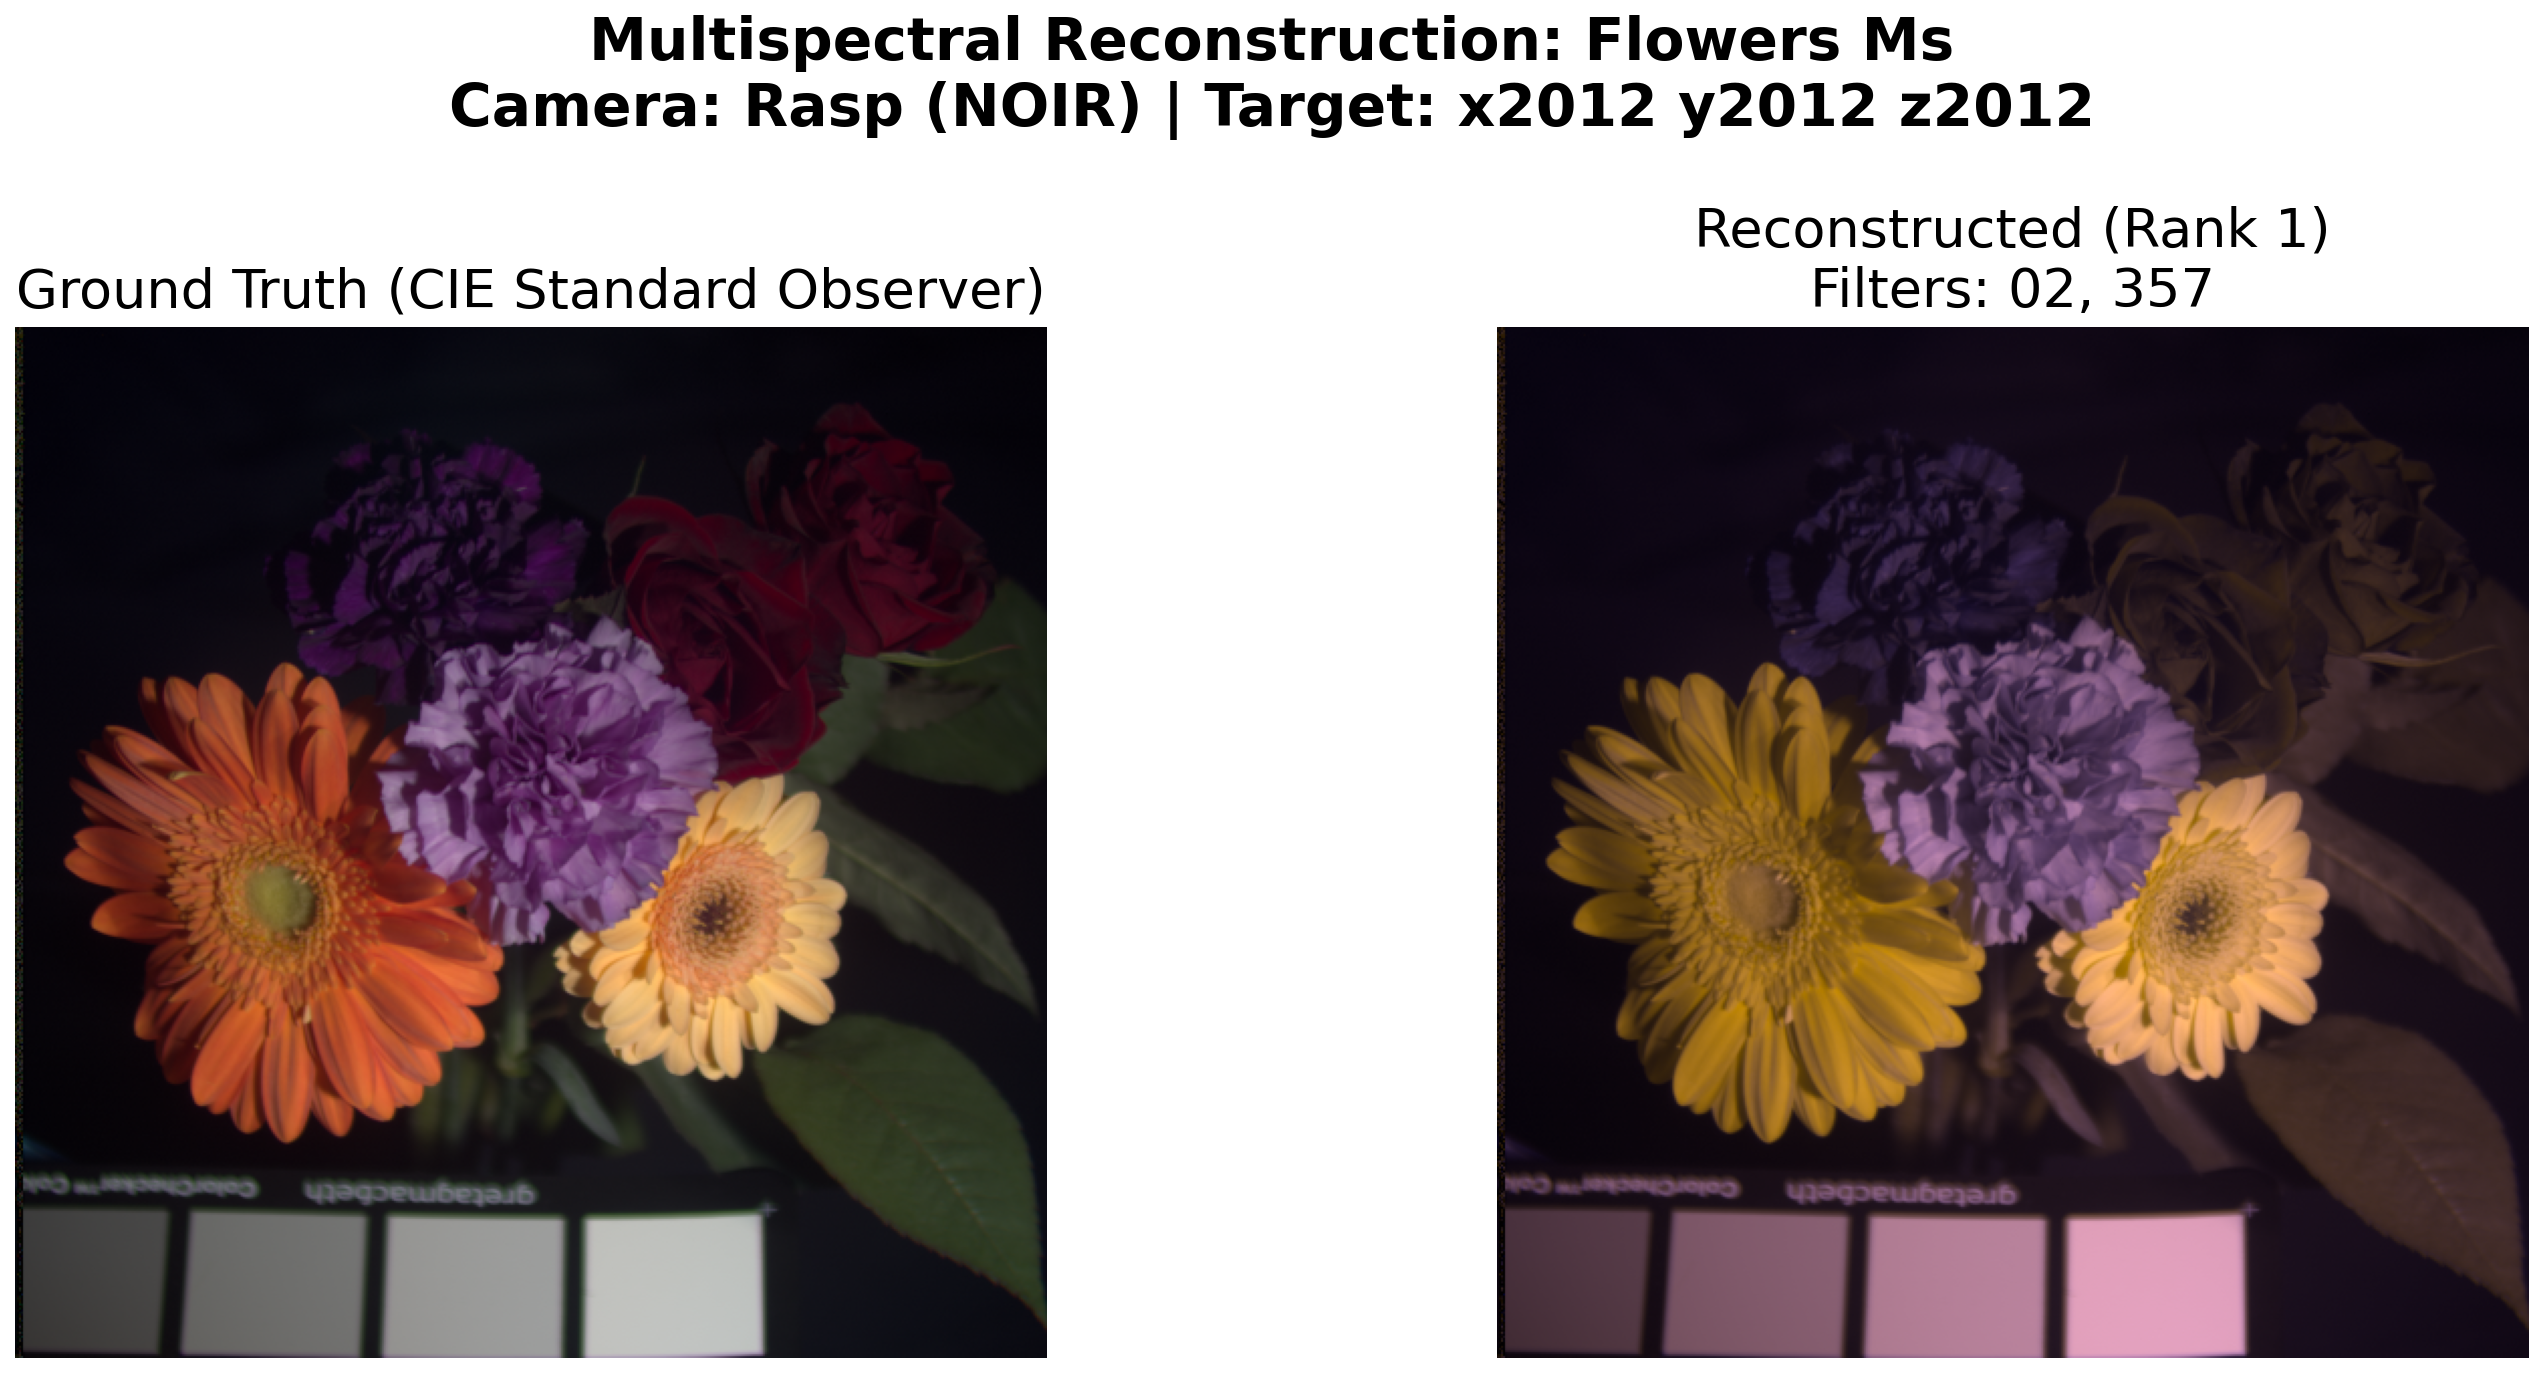
\includegraphics[width=\linewidth]{media/cave_appendix/k2flowers.png}
    \caption{$k=2$, $\dE$=13.17}
\end{subfigure}
\begin{subfigure}{.49\linewidth}
    \centering
    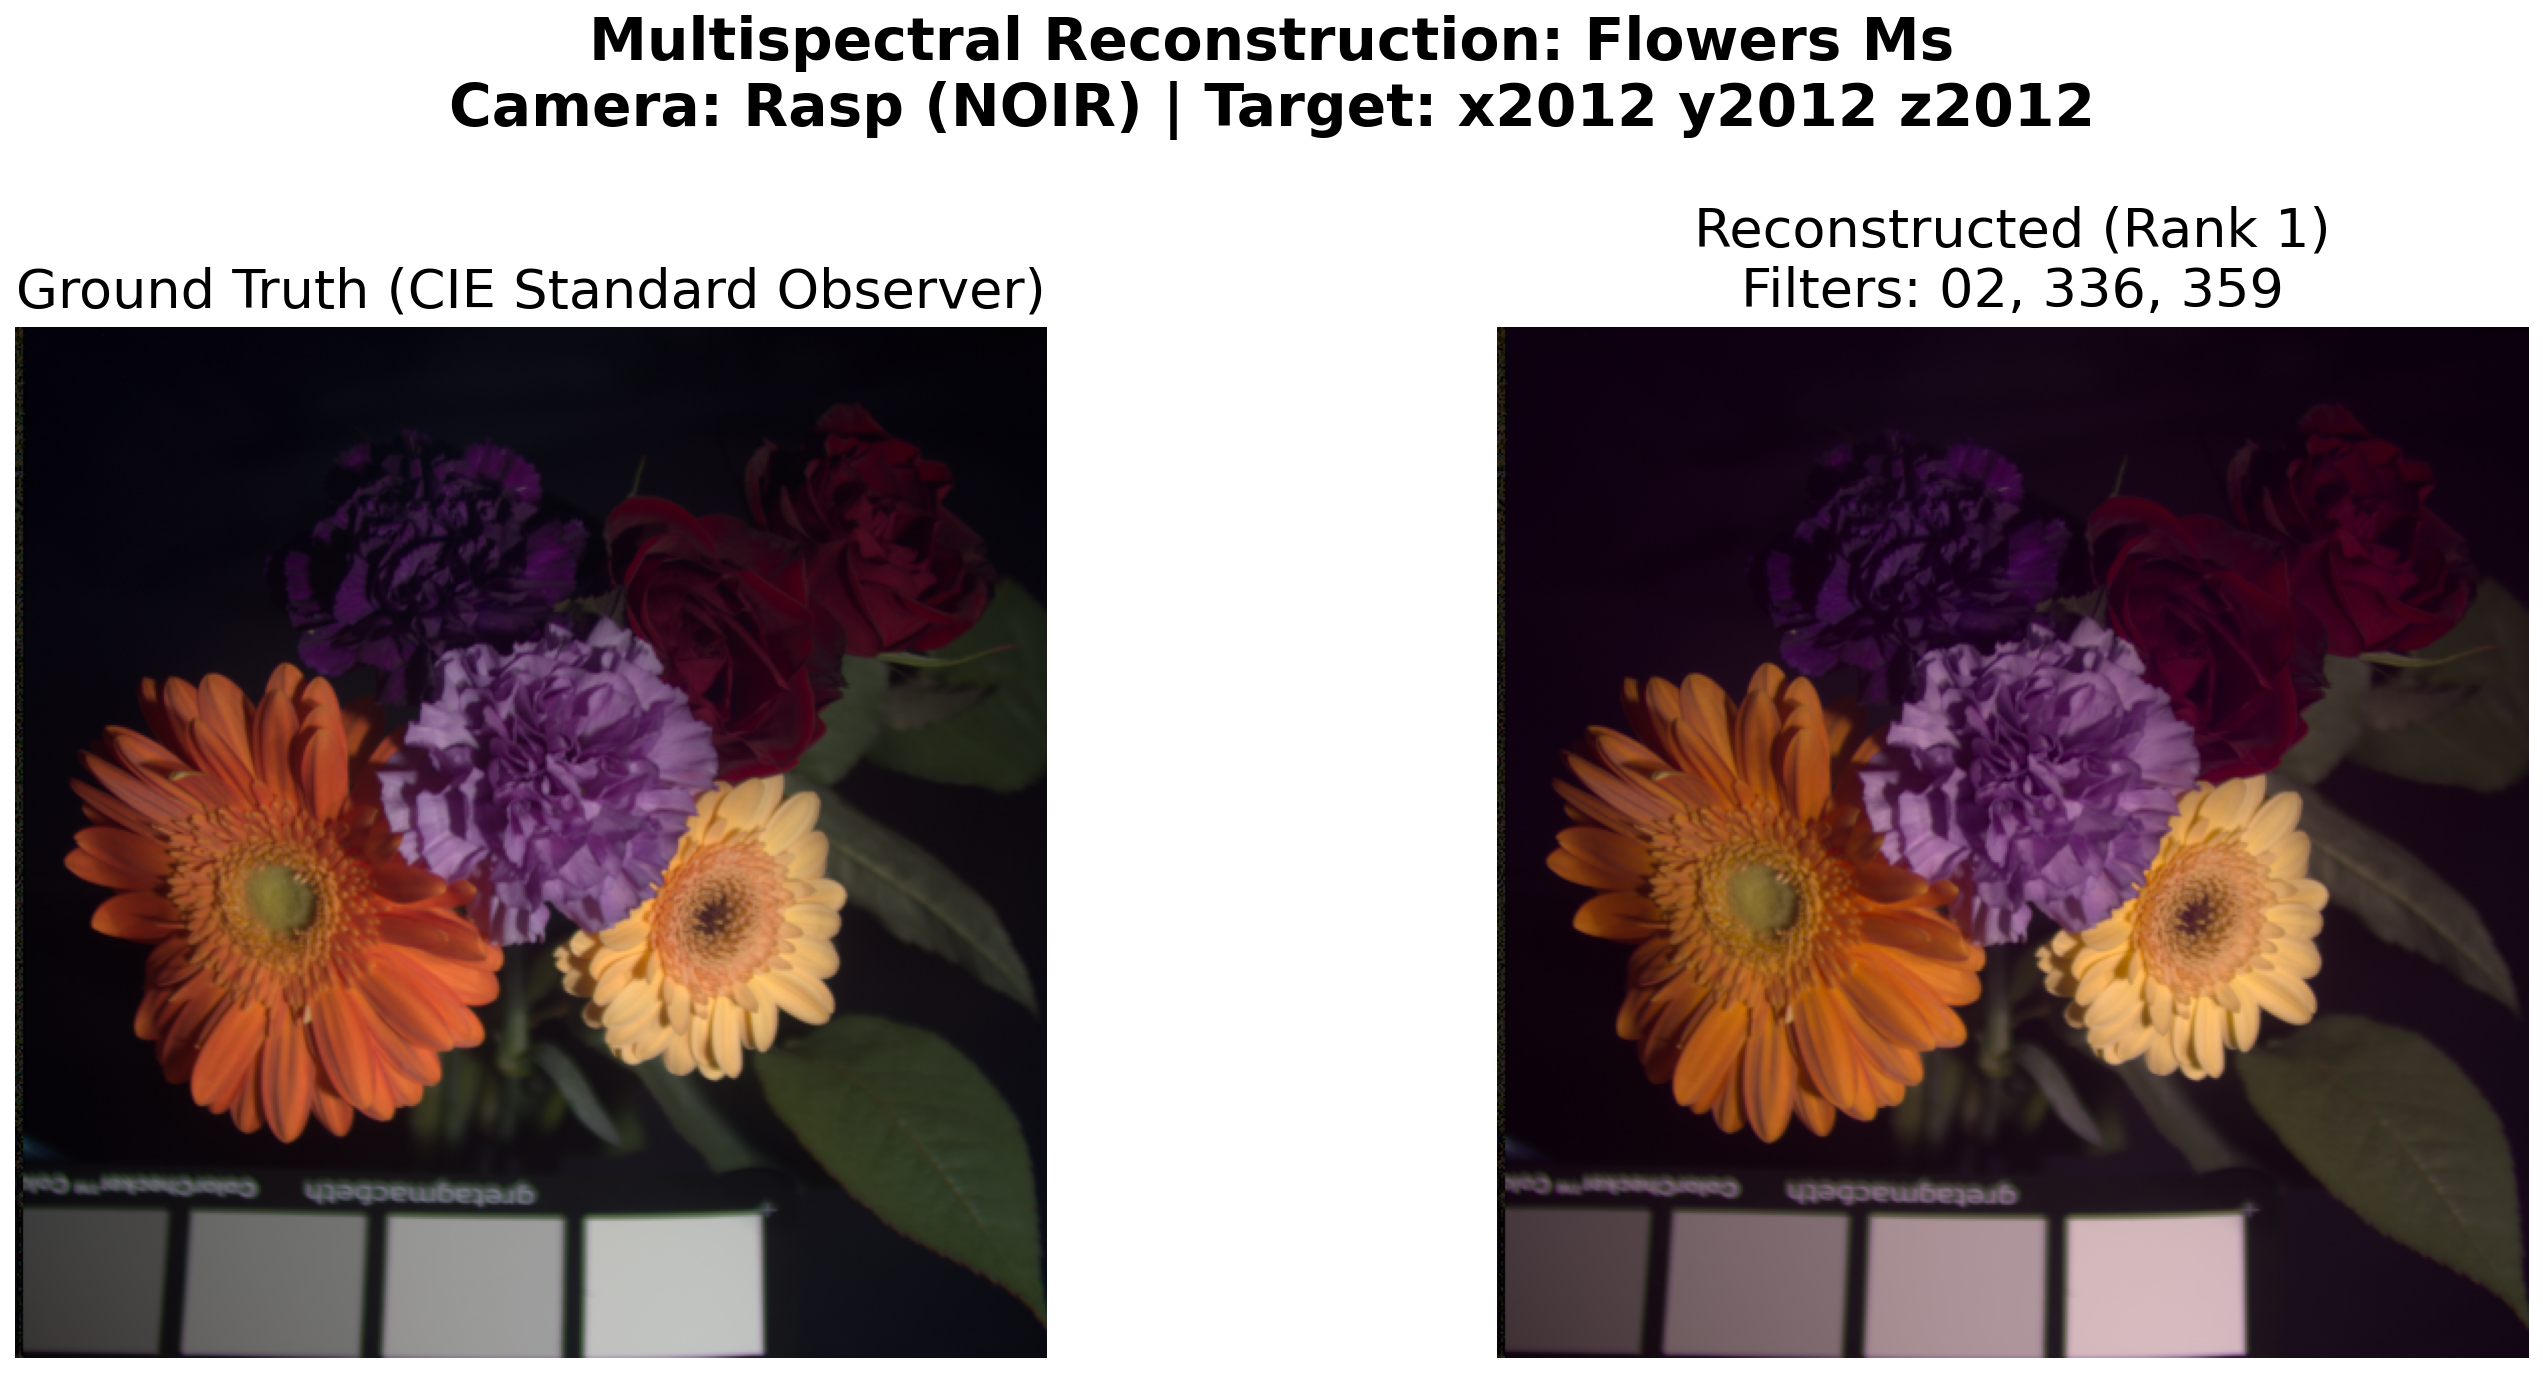
\includegraphics[width=\linewidth]{media/cave_appendix/k3flowers.png}
    \caption{$k=3$, $\dE$=5.45}
\end{subfigure}
\begin{subfigure}{.49\linewidth}
    \centering
    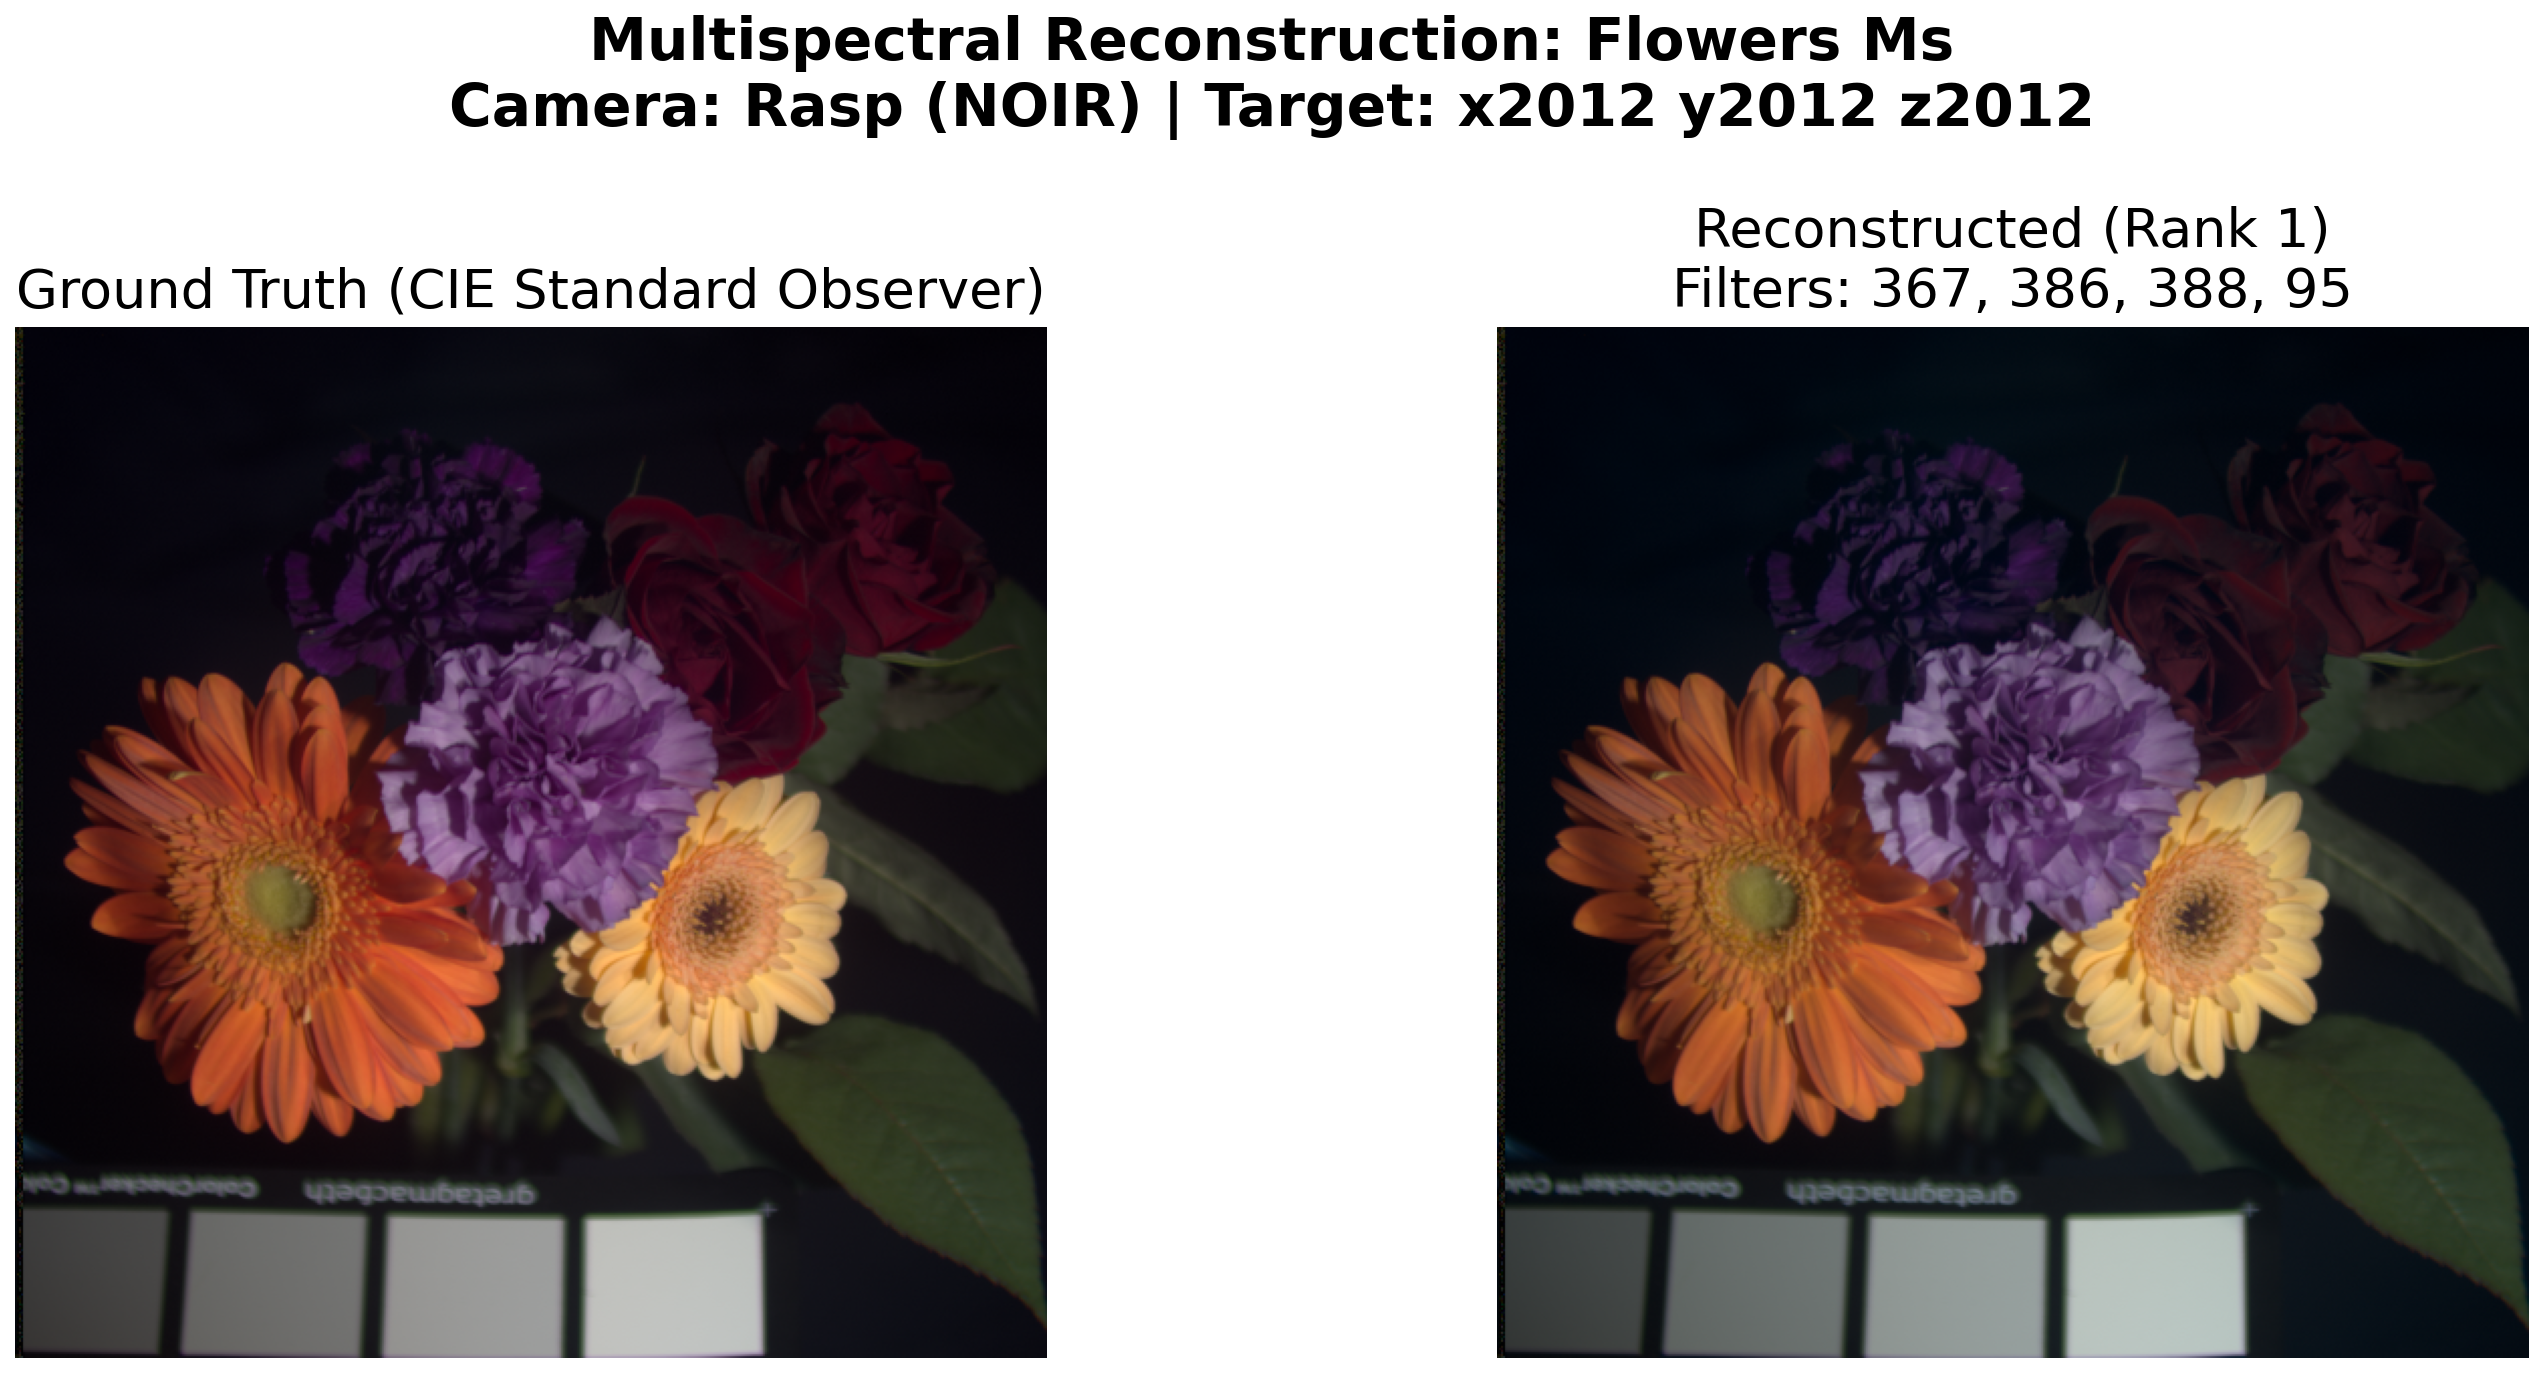
\includegraphics[width=\linewidth]{media/cave_appendix/k4flowers.png}
    \caption{$k=4$, $\dE$=1.93}
\end{subfigure}
\begin{subfigure}{.49\linewidth}
    \centering
    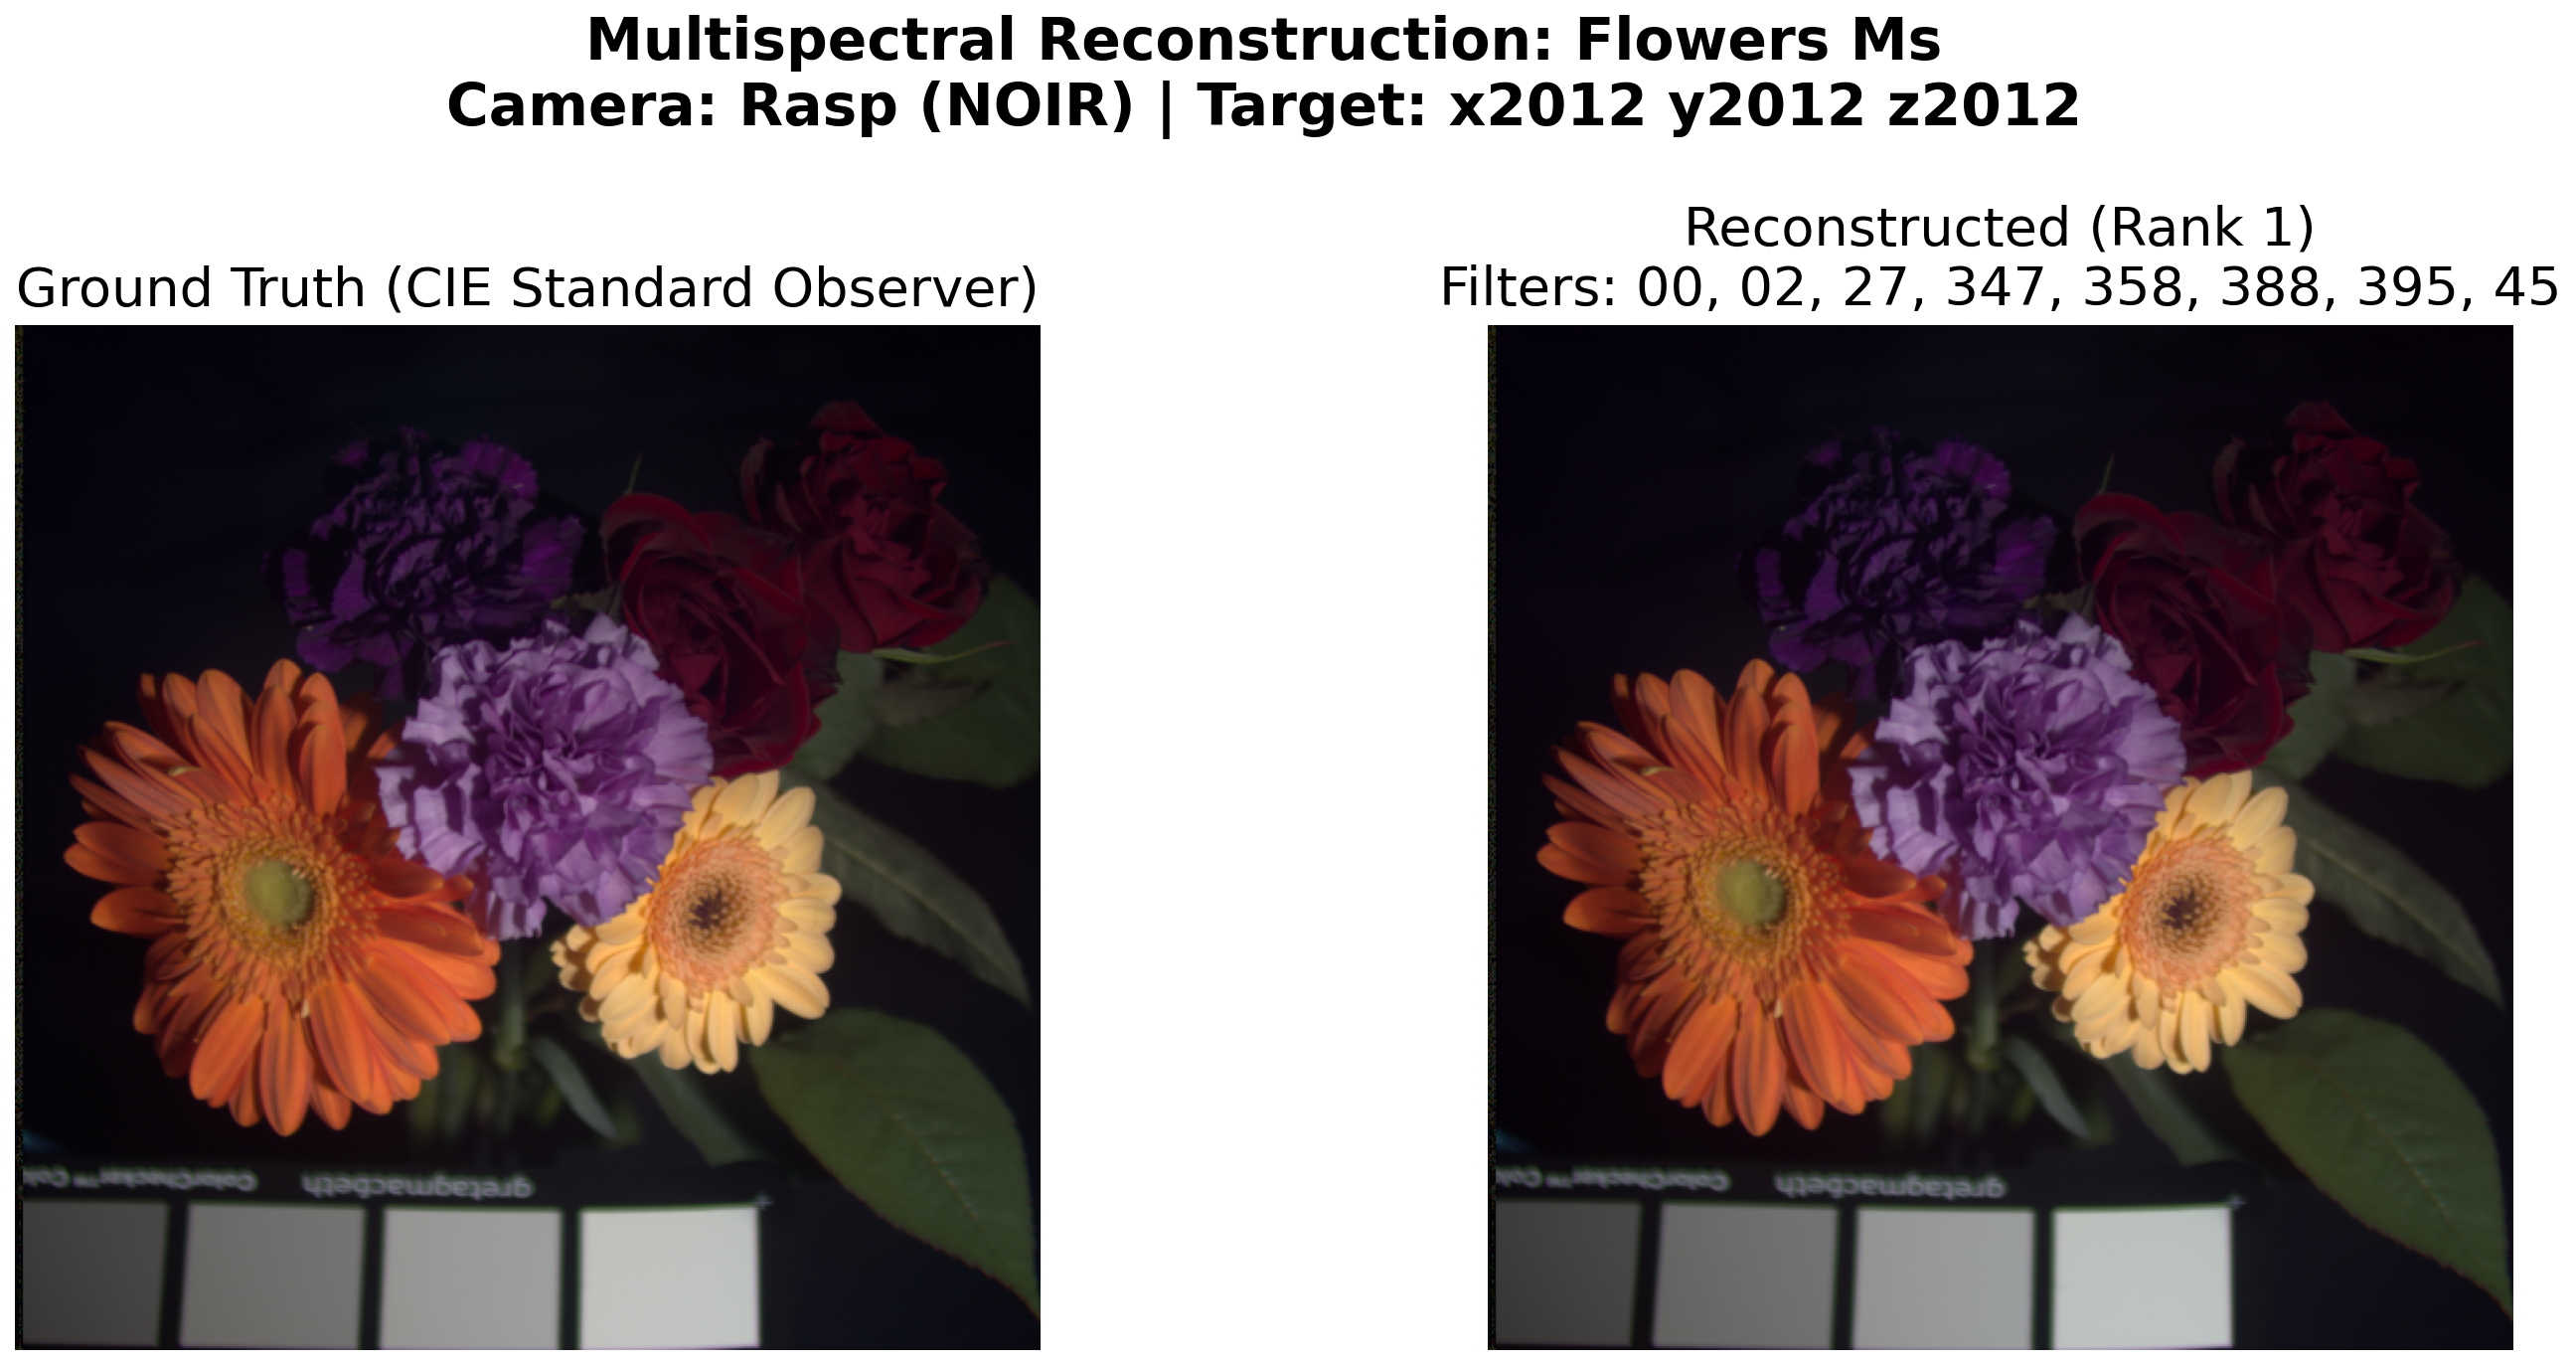
\includegraphics[width=\linewidth]{media/cave_appendix/k8flowers.png}
    \caption{$k=8$, $\dE$=.61}
\end{subfigure}
\caption{CAVE Renders of Flowers Multispectral Dataset, With Macbeth $\dE$}
\end{figure}

\subsection{Capture Errors}

A few captures in the lab featured artifacts, and a number of filters preserved transmission fairly uniformly across $\omega$ but included 'frost' or 'blur' effects which occasionally performed well in simulations but often added poor elements to reconstructions.
A number of otherwise good captures included slight lens flare near the top of the capture or just above the car, these were included as they do not affect the measurement of the PMC. 
These filters numbered $\{0, 1, 100, 101, 104, 121, 122, 124, 125, 126, 127, 160, 61, 63\}$ were excluded from the main simulation set, and another round of simulations were run with the trimmed set. 
This had negligible effect on the quality of reconstruction. 

\begin{figure}[H]
\centering
\begin{subfigure}{.49\linewidth}
    \centering
    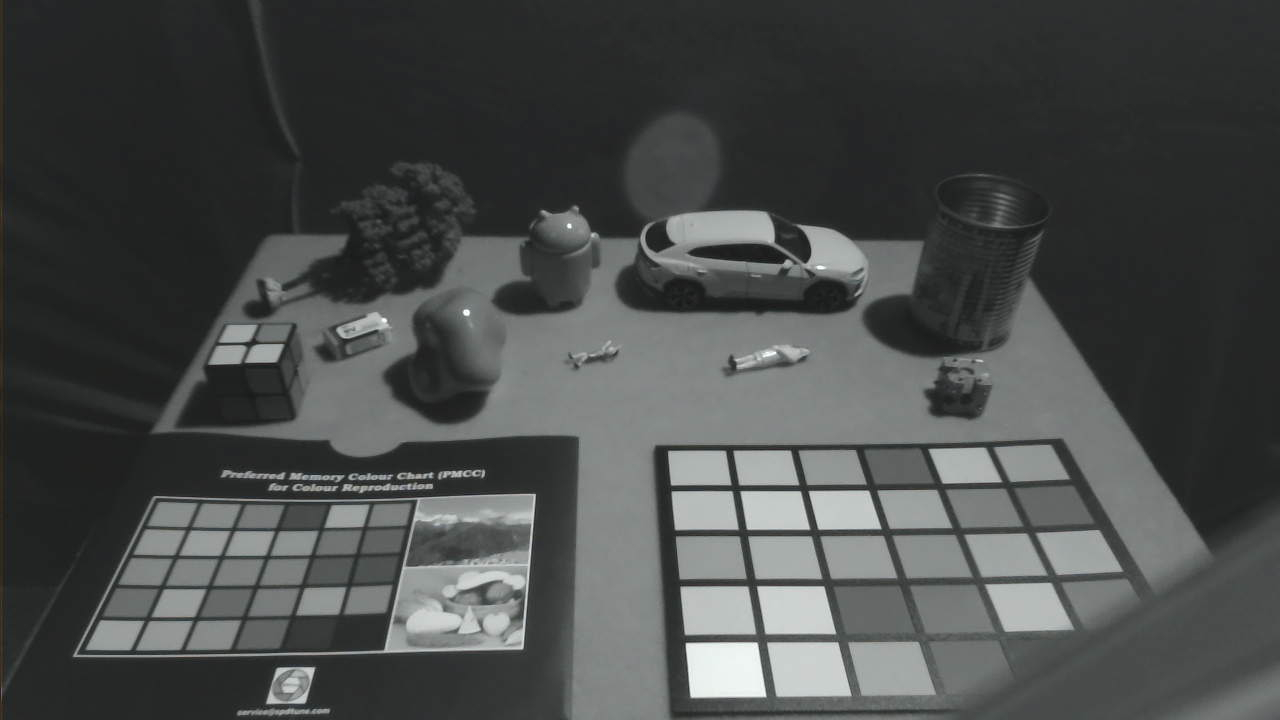
\includegraphics[width=\linewidth]{media/Lab00.jpg}
    \caption{Filter 00 in RaspberryPi Camera, excluded for artifacts in bottom right}
\end{subfigure}
\begin{subfigure}{.49\linewidth}
    \centering
    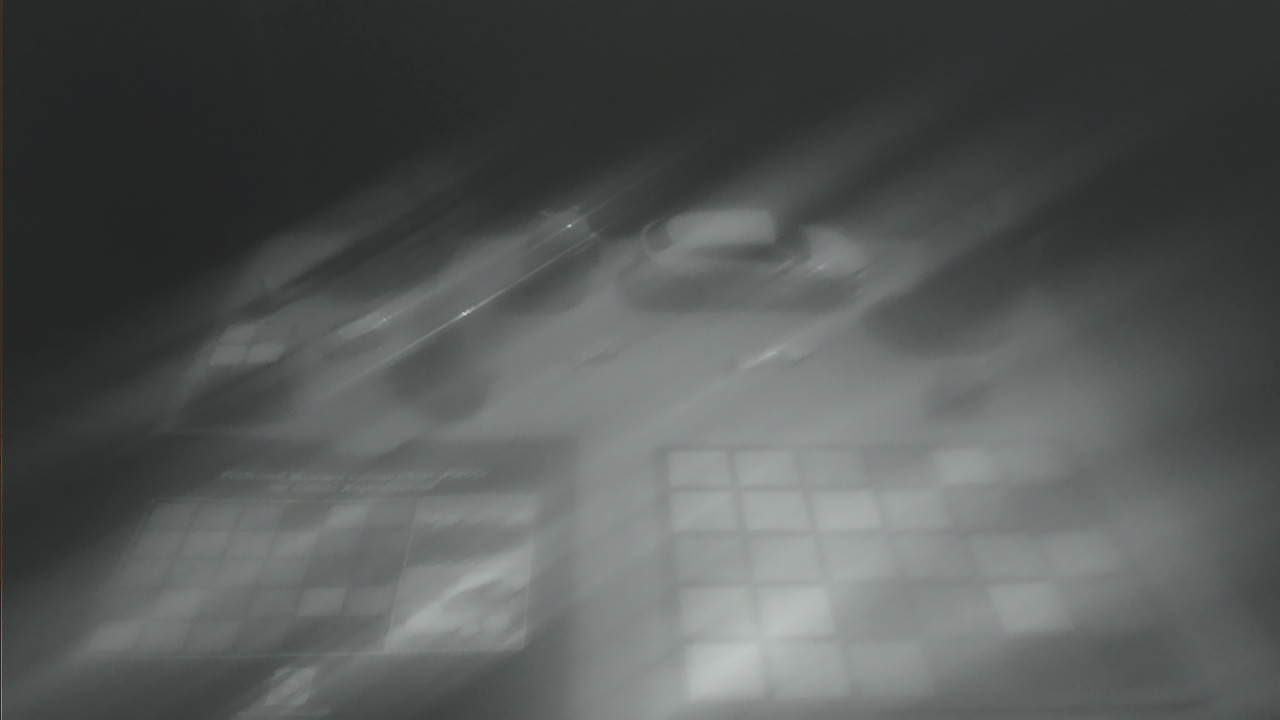
\includegraphics[width=\linewidth]{media/Lab104.jpg}
    \caption{Filter 104 in RaspberryPi Camera, excluded for blur effect}
\end{subfigure}
\begin{subfigure}{.49\linewidth}
    \centering
    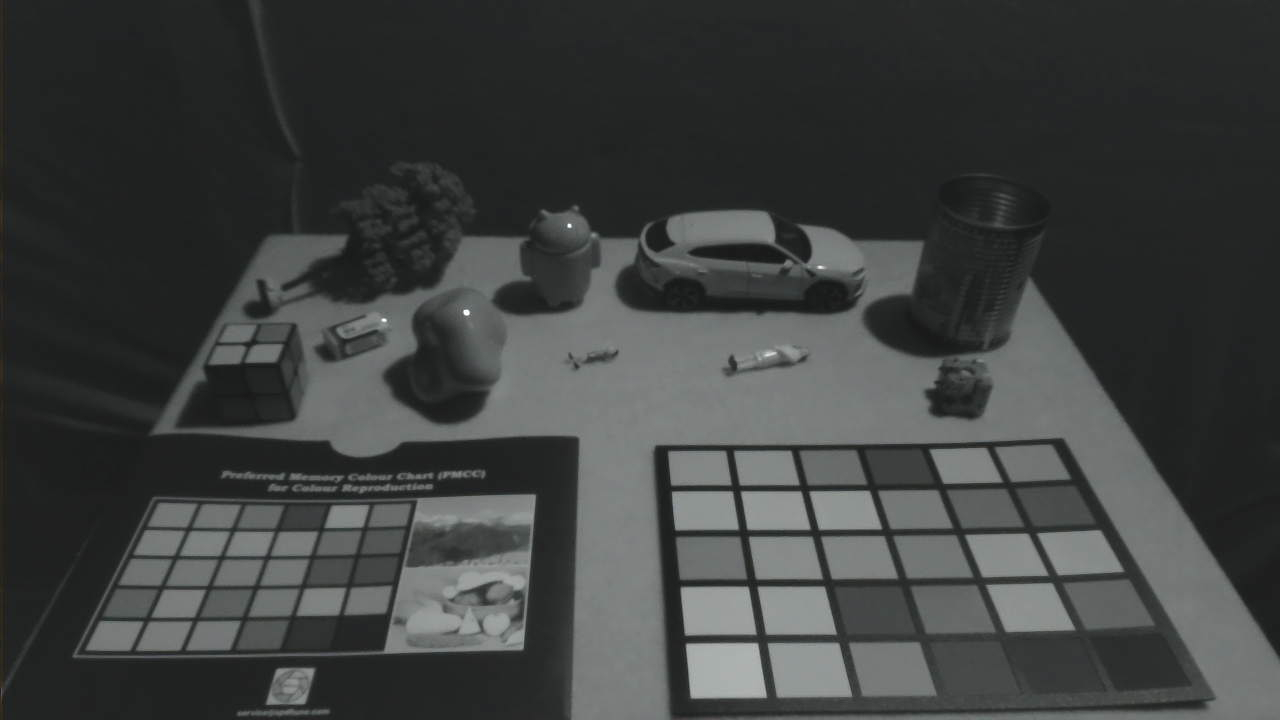
\includegraphics[width=\linewidth]{media/Lab47.jpg}
    \caption{Filter 47 in RaspberryPi Camera}
\end{subfigure}
\begin{subfigure}{.49\linewidth}
    \centering
    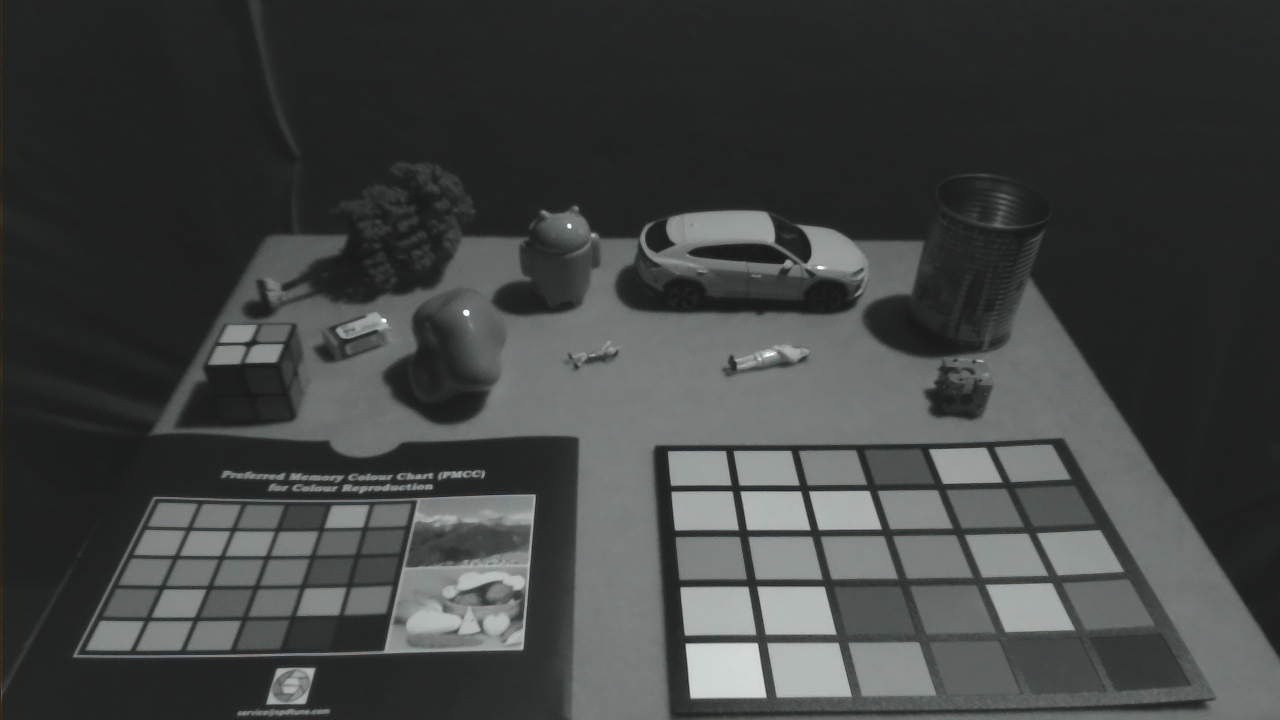
\includegraphics[width=\linewidth]{media/Lab336.jpg}
    \caption{Filter 336 in RaspberryPi Camera}
\end{subfigure}
\caption{Monochrome Captures in Lab Environment}
\end{figure}

For demonstration, we show a reconstruction for the $k=5$ case, where we simulate the optimal reconstruction including an IR-cut camera. 
However, the lab measurements were taken in the absence of an IR-cut camera, resulting in an ill-fitting reconstruction.

\begin{center}
    \centering
    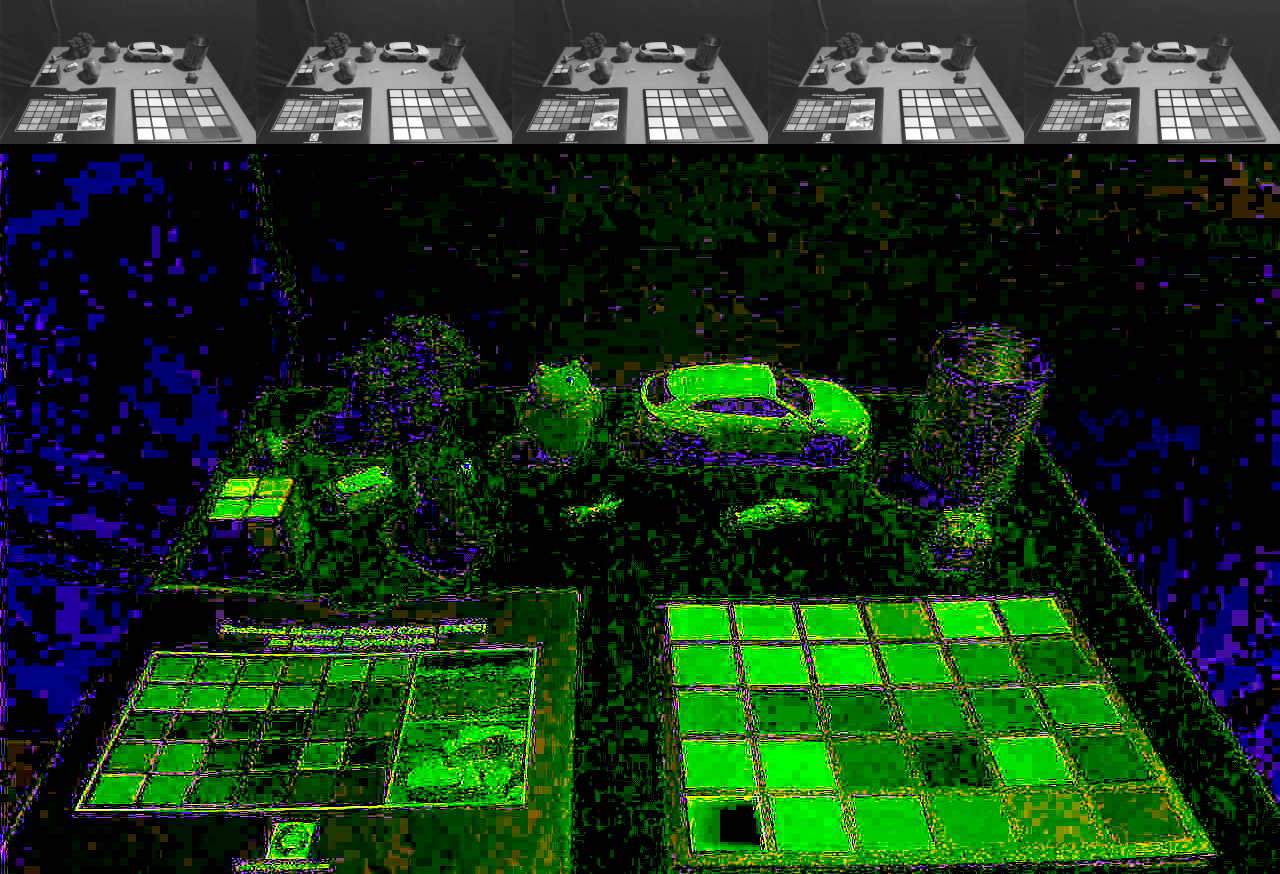
\includegraphics[width=.75\linewidth]{media/k1_5_recon_badNOIR.png}
    \captionof{figure}{$k_1=5$ Photo Lab Reconstruction with component captures above, incorrect camera configuration}
\end{center}


\subsection{In-Lab Camera Tuning}

%TODO: MOVE TO APPENDIX???
We demonstrate a poorly tuned simulation, in which we run an optimal filter selection in the presence of an IR-cut filter, but our set of captures does not include this apparatus. 
This poor example shows a different $k=5$ solution, but with the poor captures included.
Capture 00 includes a blockage in the bottom right squares in the PMC, and is therefore unfit, while filters 100 and 160 have generally poor  

\begin{figure}[H]
\centering
\begin{subfigure}{.49\linewidth}
    \centering
    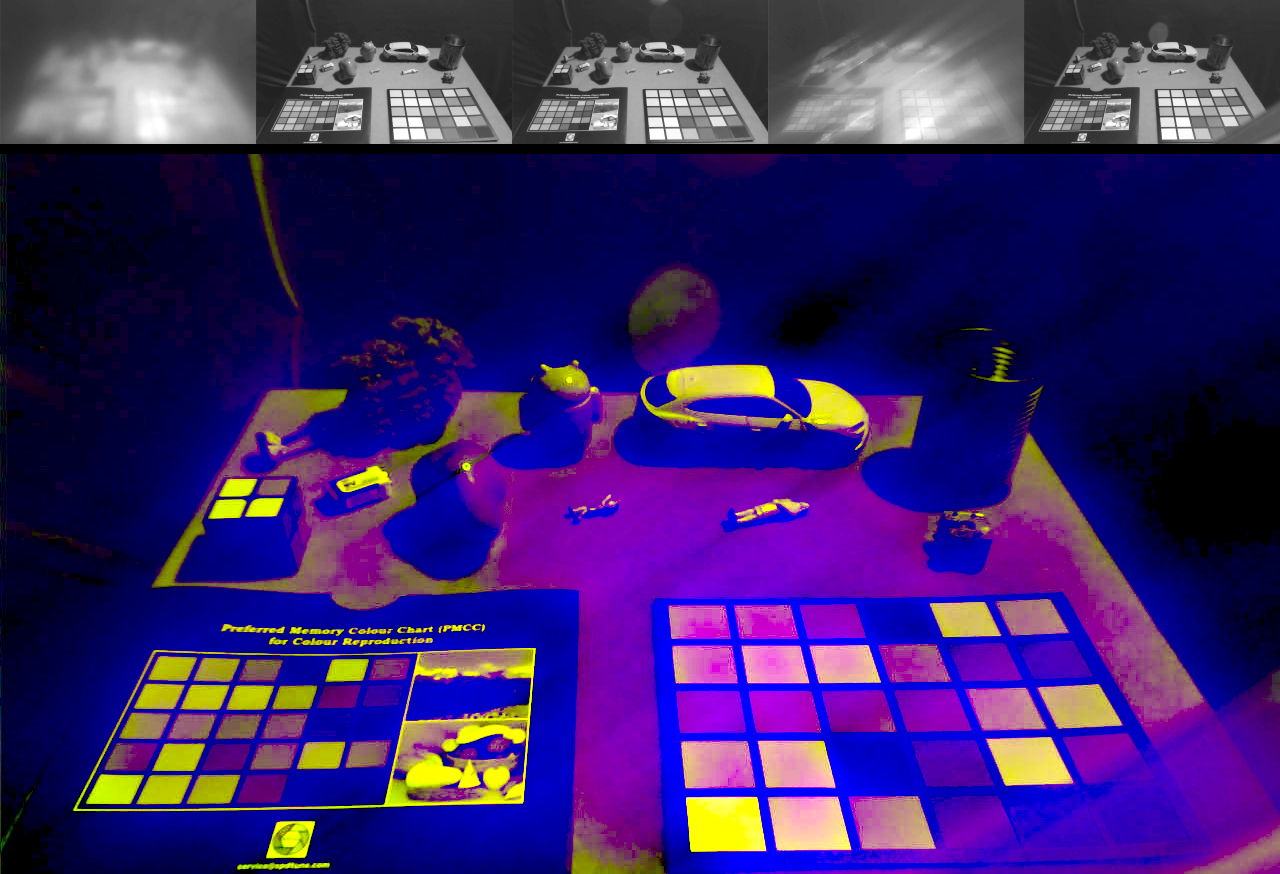
\includegraphics[width=\linewidth]{media/k5_noisy_render.png}
    \caption{Poor quality $k=5$ reconstruction including unfit filters 00, 100, 160}
\end{subfigure}
\begin{subfigure}{.49\linewidth}
    \centering
    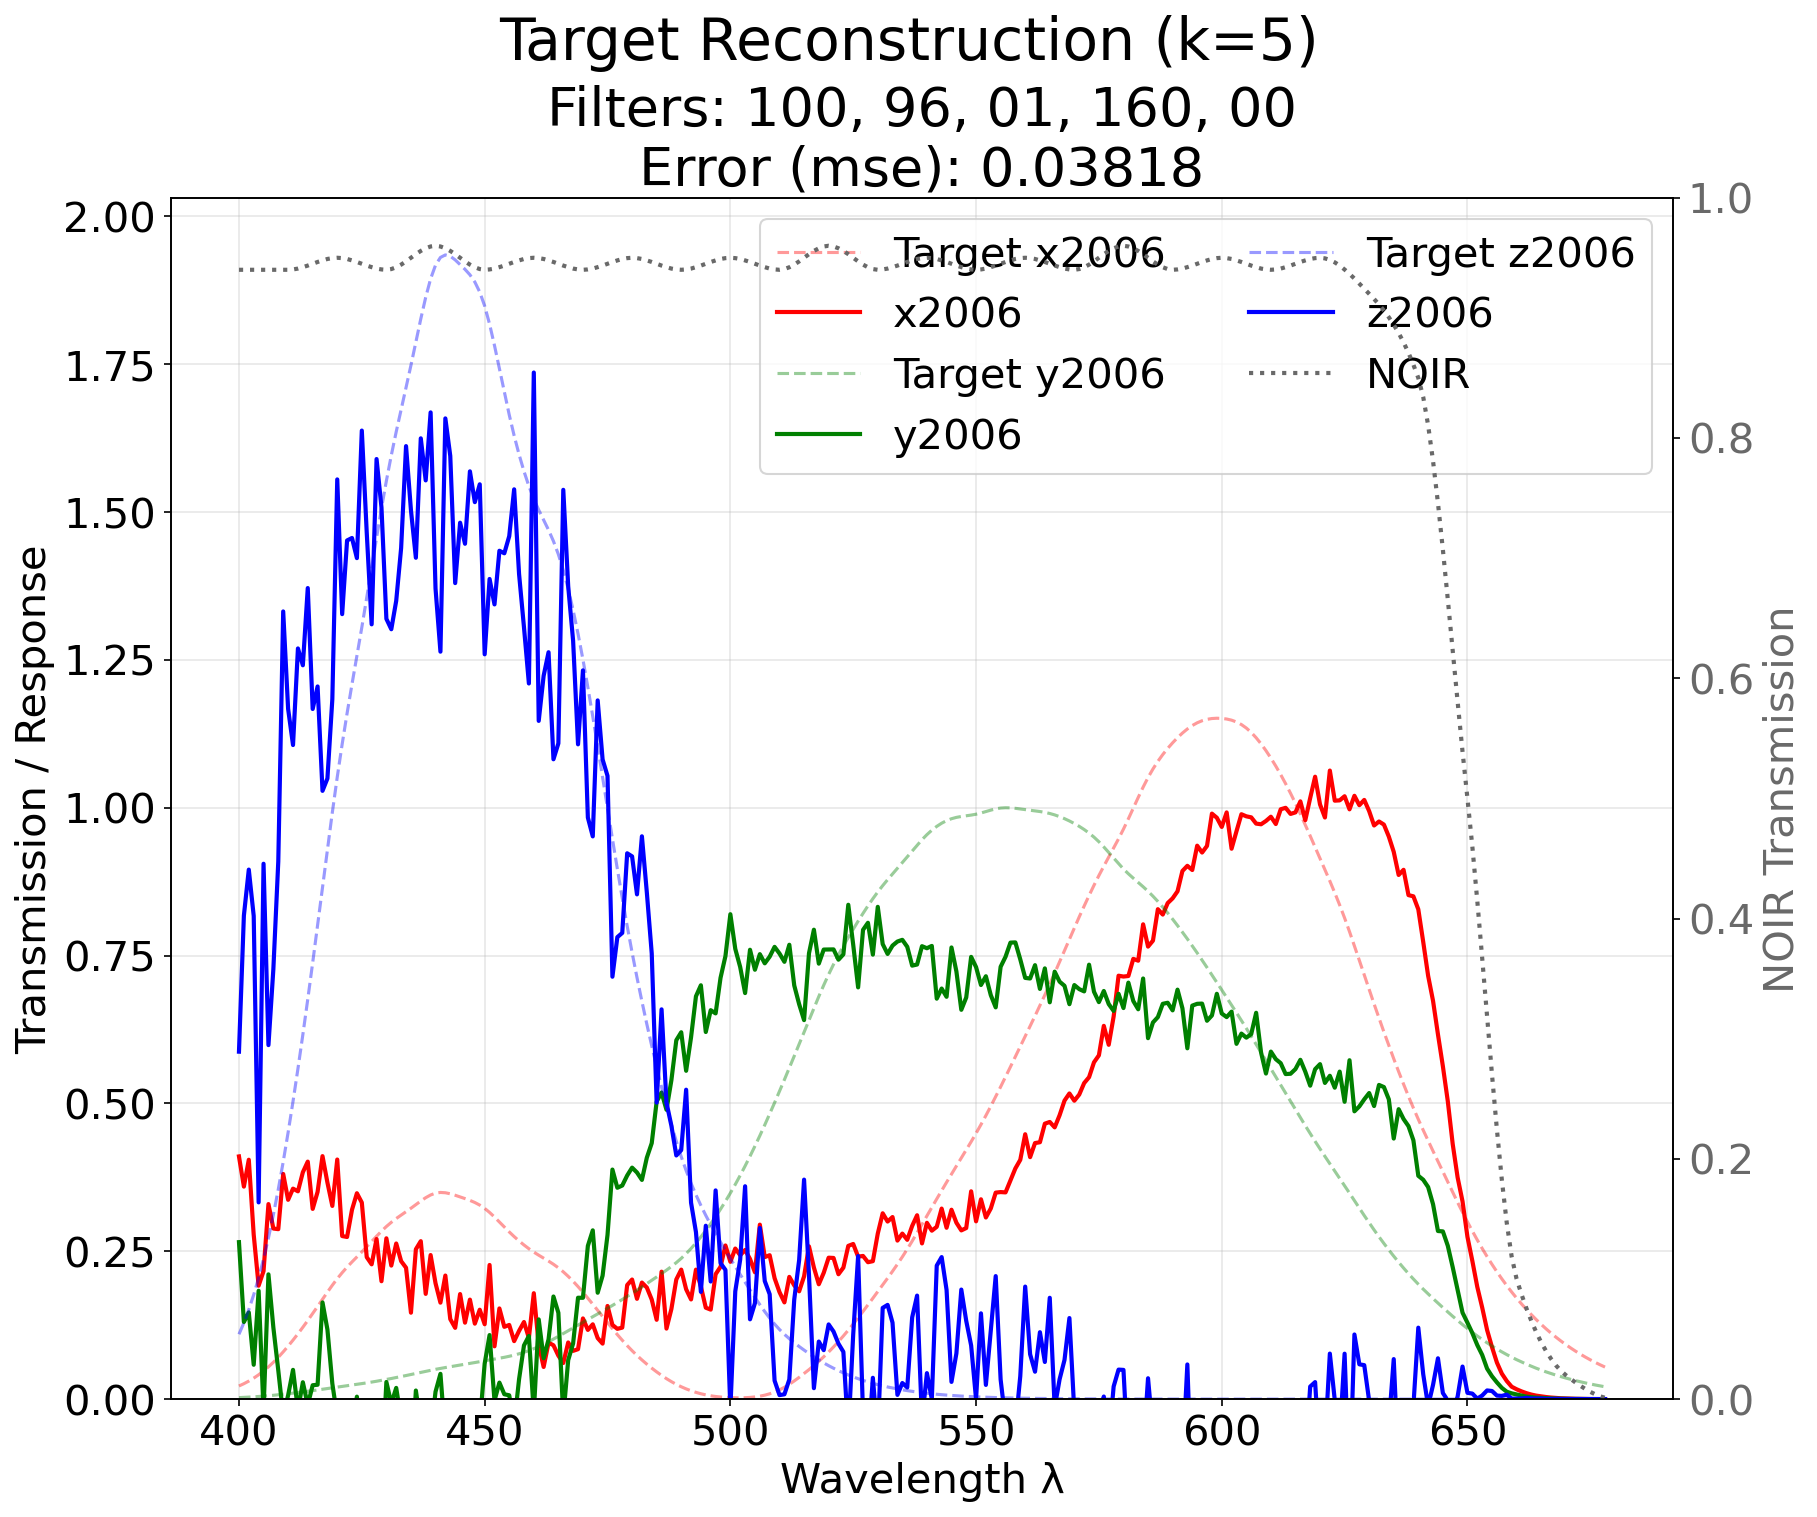
\includegraphics[width=\linewidth]{media/k5_noisy_spectra.png}
    \caption{Spectral reconstruction for $k=5$ combination with low MSE, poor realized result}
\end{subfigure}
\caption{$k=5$ filter combination with poor reconstruction quality}
\end{figure}

%TODO: if this result doesn't improve, move to appendix and explain
We also demonstrate a classical camera tuning methodology, where we minimize explicitly the average $\dE$ over the PMC. 
For $k=3$, we achieve $\dE$ of 12, which is significantly above the just-noticeable-difference threshold and warrants further investigation of potential measurement errors.
Either way, we use the simulated results for our main reconstruction efforts. 

%TODO: Improve this reconstruction
\begin{center}
    \centering
    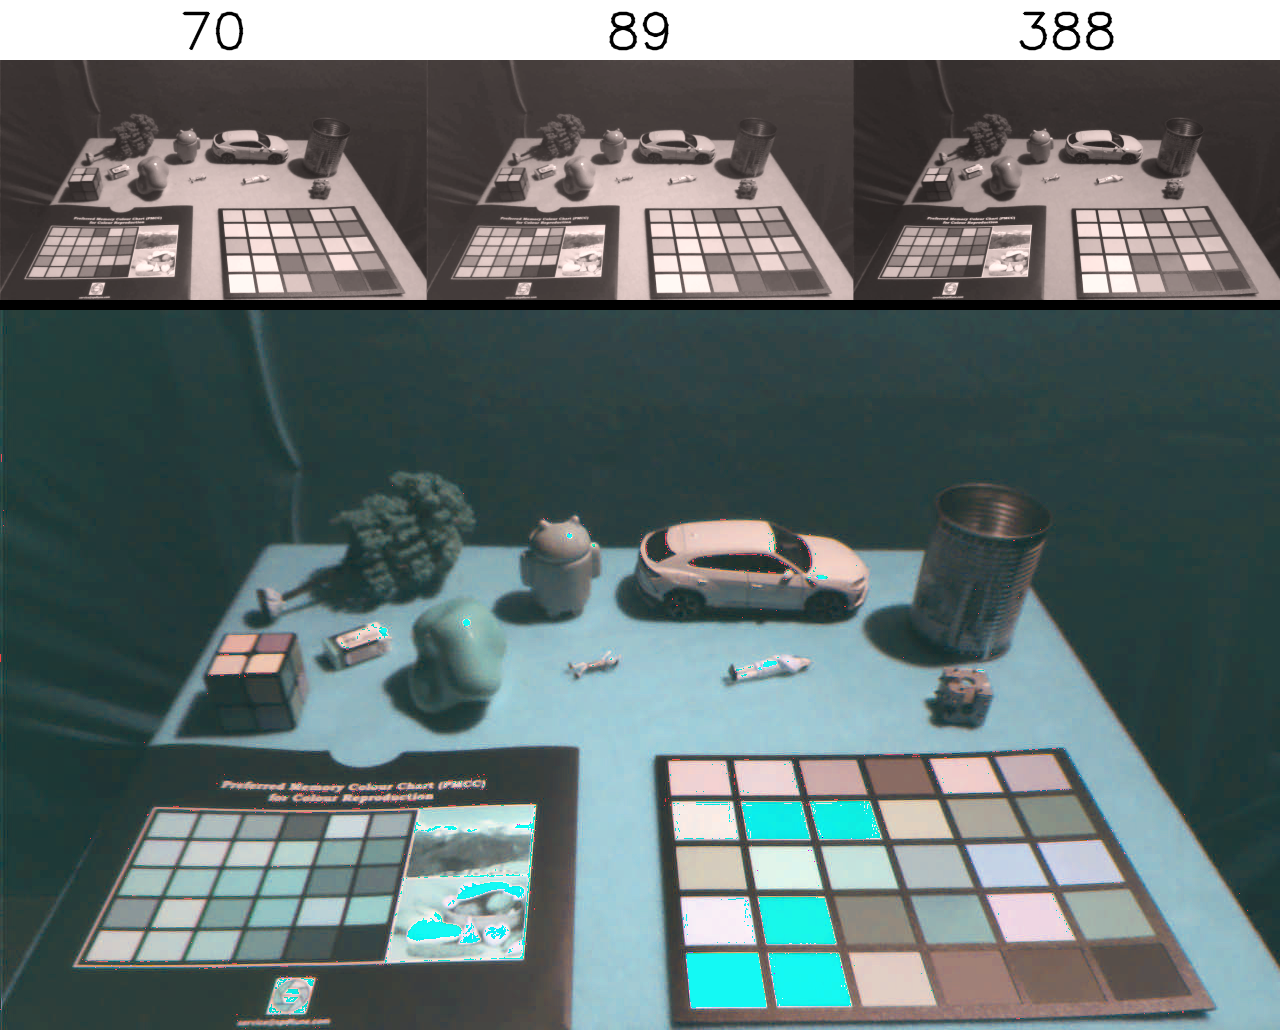
\includegraphics[width=.75\linewidth]{media/OK_recon_with_sources_70_89_388.png}
    \captionof{figure}{$k=3$ reconstruction with $\dE$ minimization}
\end{center}

\end{document}





